\documentclass[a4paper,10pt]{article}

\usepackage[utf8]{inputenc}
\usepackage{CJKutf8}
\usepackage{graphicx}
\usepackage{amsmath}
\graphicspath{ {images/} }






% For C# code
\usepackage[T1]{fontenc}
\usepackage[scaled]{beramono}

\usepackage{color}
\definecolor{bluekeywords}{rgb}{0.13,0.13,1}
\definecolor{greencomments}{rgb}{0,0.5,0}
\definecolor{redstrings}{rgb}{0.9,0,0}

\usepackage{listings}
\lstset{language=[Sharp]C,
showspaces=false,
showtabs=false,
breaklines=true,
showstringspaces=false,
breakatwhitespace=true,
escapeinside={(*@}{@*)},
commentstyle=\color{greencomments},
keywordstyle=\color{bluekeywords}\bfseries,
stringstyle=\color{redstrings},
basicstyle=\ttfamily
}






%For python code
\usepackage{listings}
\usepackage{color}

%New colors defined below
\definecolor{codegreen}{rgb}{0,0.6,0}
\definecolor{codegray}{rgb}{0.5,0.5,0.5}
\definecolor{codepurple}{rgb}{0.58,0,0.82}
\definecolor{backcolour}{rgb}{0.95,0.95,0.92}

%Code listing style named "mystyle"
\lstdefinestyle{mystyle}{
  backgroundcolor=\color{backcolour},   commentstyle=\color{codegreen},
  keywordstyle=\color{magenta},
  numberstyle=\tiny\color{codegray},
  stringstyle=\color{codepurple},
  basicstyle=\footnotesize,
  breakatwhitespace=false,         
  breaklines=true,                 
  captionpos=b,                    
  keepspaces=true,                 
  numbers=left,                    
  numbersep=5pt,                  
  showspaces=false,                
  showstringspaces=false,
  showtabs=false,                  
  tabsize=2
}

%"mystyle" code listing set
\lstset{style=mystyle}



\title{Cracking leetcode in Python}
\author{XIN LIU \\ liux4@oregonstate.edu}
 


\begin{document}

% Table of Contents
\tableofcontents

\maketitle

%%%%%%%%%%%%%%%%%%%%%%%%%%%%%%%%%%%%%%%%%%%%%%%%%%%%%%%%%%%%%%%%%%%%%%%%%%%%%
%%%%%%%%%%%%%%%%%%%%%%%%%%%%%  Introduction  %%%%%%%%%%%%%%%%%%%%%%%%%%%%%%%%
%%%%%%%%%%%%%%%%%%%%%%%%%%%%%%%%%%%%%%%%%%%%%%%%%%%%%%%%%%%%%%%%%%%%%%%%%%%%%

\noindent The motivation of this little e-book is to share some ideas with and expect comments from people who have common interests in cracking algorithm questions for technical interview. The questions discussed and demonstrated here are all from the famous interview training website, \textbf{leetcode.com}. In the first version, we share our analyses and solutions of around 147 questions in total. All code snippets are in Python. That's why "in Python" appears in the title of the e-book. And all code are accepted on leetcode.com. We welcome and encourage you to give us your feedback and meanwhile share your solutions in different programming languages. We establed a github repo for this e-book, because we want to open source all data related to the e-book to everyone.\\

\noindent As our first motivation of the e-book is to assist Chinese college students to prepare their future job interview, we described our ideas only in Chinese. In the future, we also plan to offer an English version for more college students.\\

\noindent Special thanks to my best friend, Jian (Andy) Zhang, for giving me a lot of positive and constructive suggestions on this little e-book and solution code.\\


\medskip

\section{Array and List}

\subsection{Array}


\subsubsection{leetcode 26. Remove Duplicates from Sorted Array}

Given a sorted array, remove the duplicates in place such that each element appear only once and return the new length. Do not allocate extra space for another array, you must do this in place with constant memory. \\

\noindent For example, Given input array nums = [1,1,2], Your function should return length = 2, with the first two elements of nums being 1 and 2 respectively. It doesn't matter what you leave beyond the new length. \\

\begin{CJK*}{UTF8}{gbsn}
\noindent 解题思路:根据题目要求,不能使用额外的存储空间,所以一定是原地去重,那么一个比较直接的想法就是用不同的值覆盖重复的值。因此,我们用一个指针$j$指向目标数组$A$当前待判断是否是重复值的元素,用另外一个指针$i$指向已经建立好的、没有重复值的序列(数组$A$的一个子序列)的末尾。如果$A[i] \neq A[j]$说明$j$当前指向的元素与新建立的序列中的元素不同,可以添加到新序列中。因此,移动$i$到下一个位置,并将$j$指向的值复制到$i$的位置。如果$A[i]==A[j]$,说明当前$j$指向的元素与新序列中的最后一个元素是重复的,不应该加到新序列中,因此移动$j$到下一个位置,继续后序的筛选,直到$j$访问完数组$A$的最后一个元素。这时,$i+1$即为最后的结果。算法的时间复杂度为$O(n)$。参考下面的示例图。\\
\noindent 这道题另外一个需要注意的地方,也是后续所有题目解题是需要注意的事项是增加边界值的验证。由于leetcode提供的代码验证,已经提供了一些测试用例,但是最好在提交代码之前,自己设计一些测试用例验证自己设计的算法和代码实现,这也是面试题目要考查应试者的一部分内容。
\end{CJK*}

\begin{figure}[h]
    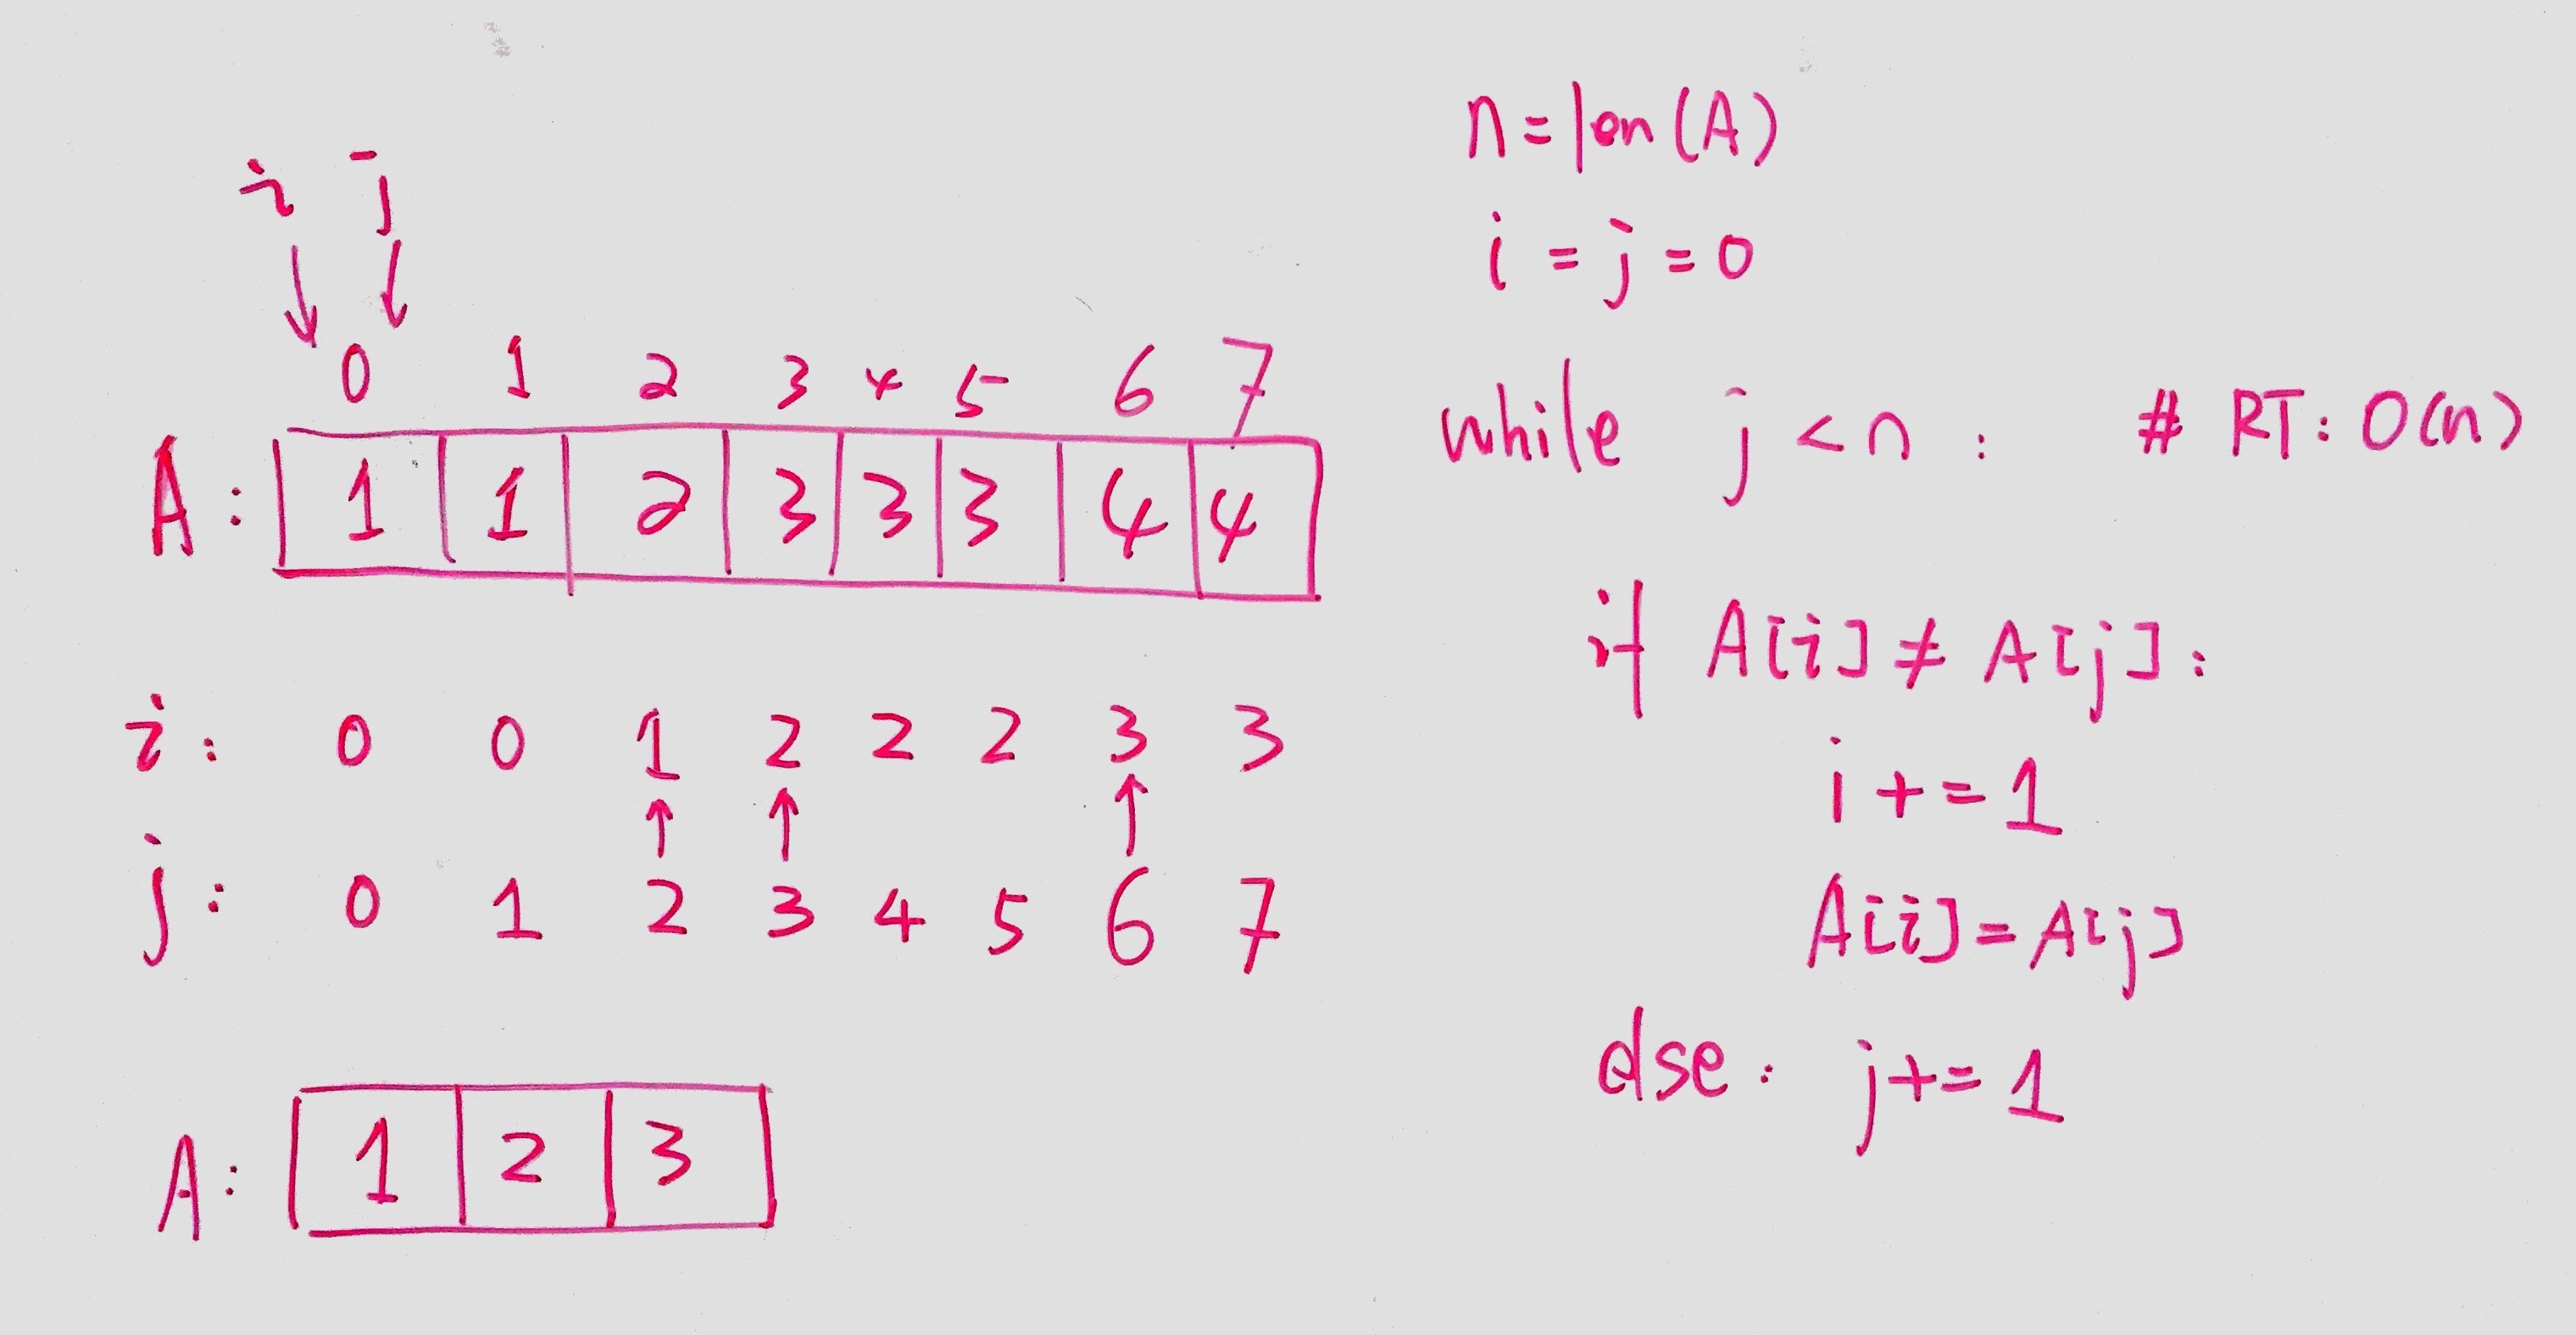
\includegraphics[width=\textwidth]{leetcode26.jpg}
    \centering\\
\end{figure}

\begin{lstlisting}[language=Python, caption=Problem26. Remove Duplicates from Sorted Array]

class Solution(object):
    def removeDuplicates(self, nums):   # RT: O(n)
        """
        :type nums: List[int]
        :rtype: int
        """
        if nums is None or len(nums) == 0:
            return 0
        slow = 0
        for fast in xrange(len(nums)):
            if nums[fast] != nums[slow]:
                slow += 1
                nums[slow] = nums[fast]
        return slow + 1
\end{lstlisting}





\subsubsection{leetcode 80. Remove Duplicates from Sorted Array II}
Follow up for "Remove Duplicates": What if duplicates are allowed at most twice? For example, Given sorted array nums = $[1,1,1,2,2,3]$, Your function should return length = 5, with the first five elements of nums being 1, 1, 2, 2 and 3. It doesn't matter what you leave beyond the new length.\\

\begin{CJK*}{UTF8}{gbsn}
\noindent 解题思路:这道题可以直接泛化为“求解一个允许存在$k$个重复值的排序数组”。当$k=2$时就是本题的情况。算法的设计与leetcode26 Remove Duplicates from Sorted Array基本一致,差别在于判断重复值的时候,需要增加偏移量$k$(代码第15行),因为允许有$k$重复值。见下图示例。
\end{CJK*}

\begin{figure}[h]
    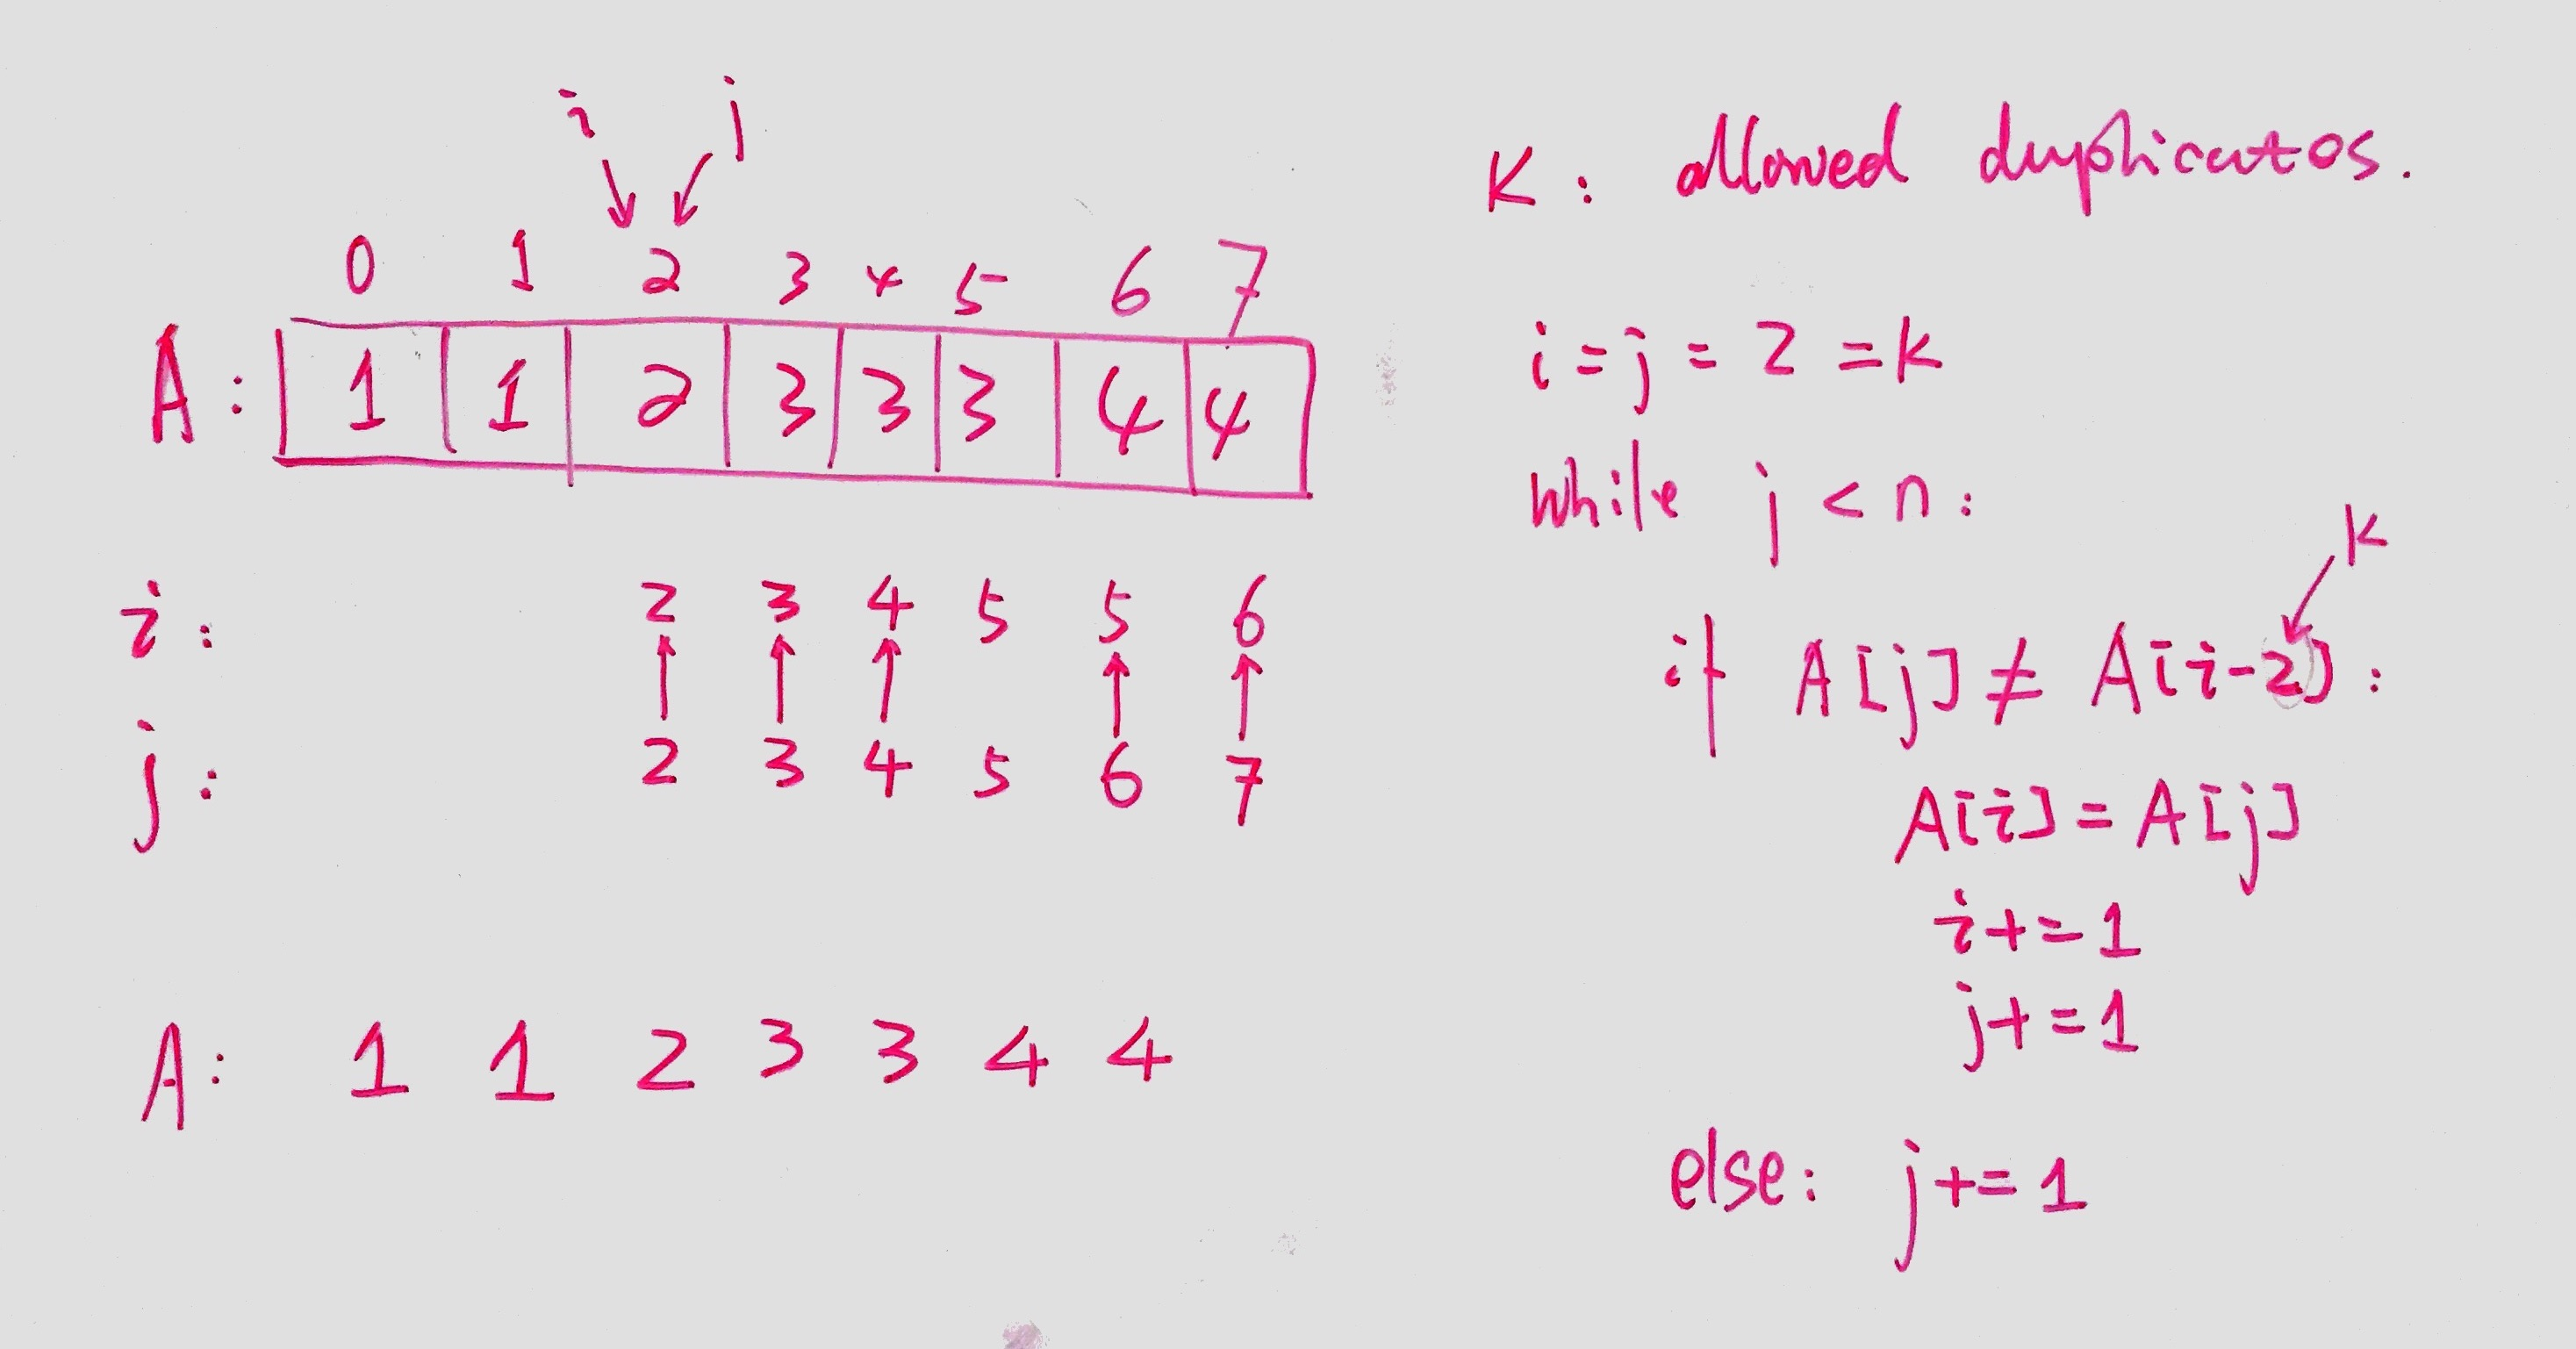
\includegraphics[width=\textwidth]{leetcode80.jpg}
    \centering\\
\end{figure}

\begin{lstlisting}[language=Python, caption=Problem80. Remove Duplicates from Sorted Array II]

class Solution(object):
    # A generic implementation for "at most k duplicates" problems
    def removeDuplicates(self, nums):  
        """
        :type nums: List[int]
        :rtype: int
        """
        if len(nums) <= 2: return len(nums)
        
        # k indicates the duplicates allowed.
        k = 2
        i = k
        for j in range(k, len(nums)):
            if nums[j] != nums[i-k]:
                nums[i] = nums[j]
                i += 1
        return i
\end{lstlisting}




\subsubsection{leetcode 33. Search in Rotated Sorted Array}
Suppose a sorted array is rotated at some pivot unknown to you beforehand. (i.e., 0 1 2 4 5 6 7 might become 4 5 6 7 0 1 2). You are given a target value to search. If found in the array return its index, otherwise return -1. You may assume no duplicate exists in the array.\\

\begin{CJK*}{UTF8}{gbsn}
\noindent 解题思路:对于在有序序列中查找指定值最有效的方法就是二叉搜索算法,时间复杂度为$O(logn)$。但是,这道题增加了一个难度,即旋转了有序序列,这样就破坏了原有的递增序列特性,从而需要改变二叉搜索排序中的判断条件。这道题的考点应该在于对二叉搜索算法的理解。\\
\end{CJK*}


\begin{lstlisting}[language=Python, caption=Problem33. Search in Rotated Sorted Array]

class Solution(object):
    def search(self, nums, target): # RT: O(log(n)), space: O(1)
        """
        :type nums: List[int]
        :type target: int
        :rtype: int
        """
        start, end = 0, len(nums)-1
        while start <= end:
            mid = (start + end)/2
            if nums[mid] == target: return mid
            if nums[start]<=nums[mid]:
                if nums[start]<=target<=nums[mid]:
                    end = mid
                else:
                    start = mid+1
            else:
                if nums[mid]<=target<=nums[end]:
                    start = mid+1
                else:
                    end = mid
        return -1
\end{lstlisting}

\begin{figure}[h]
    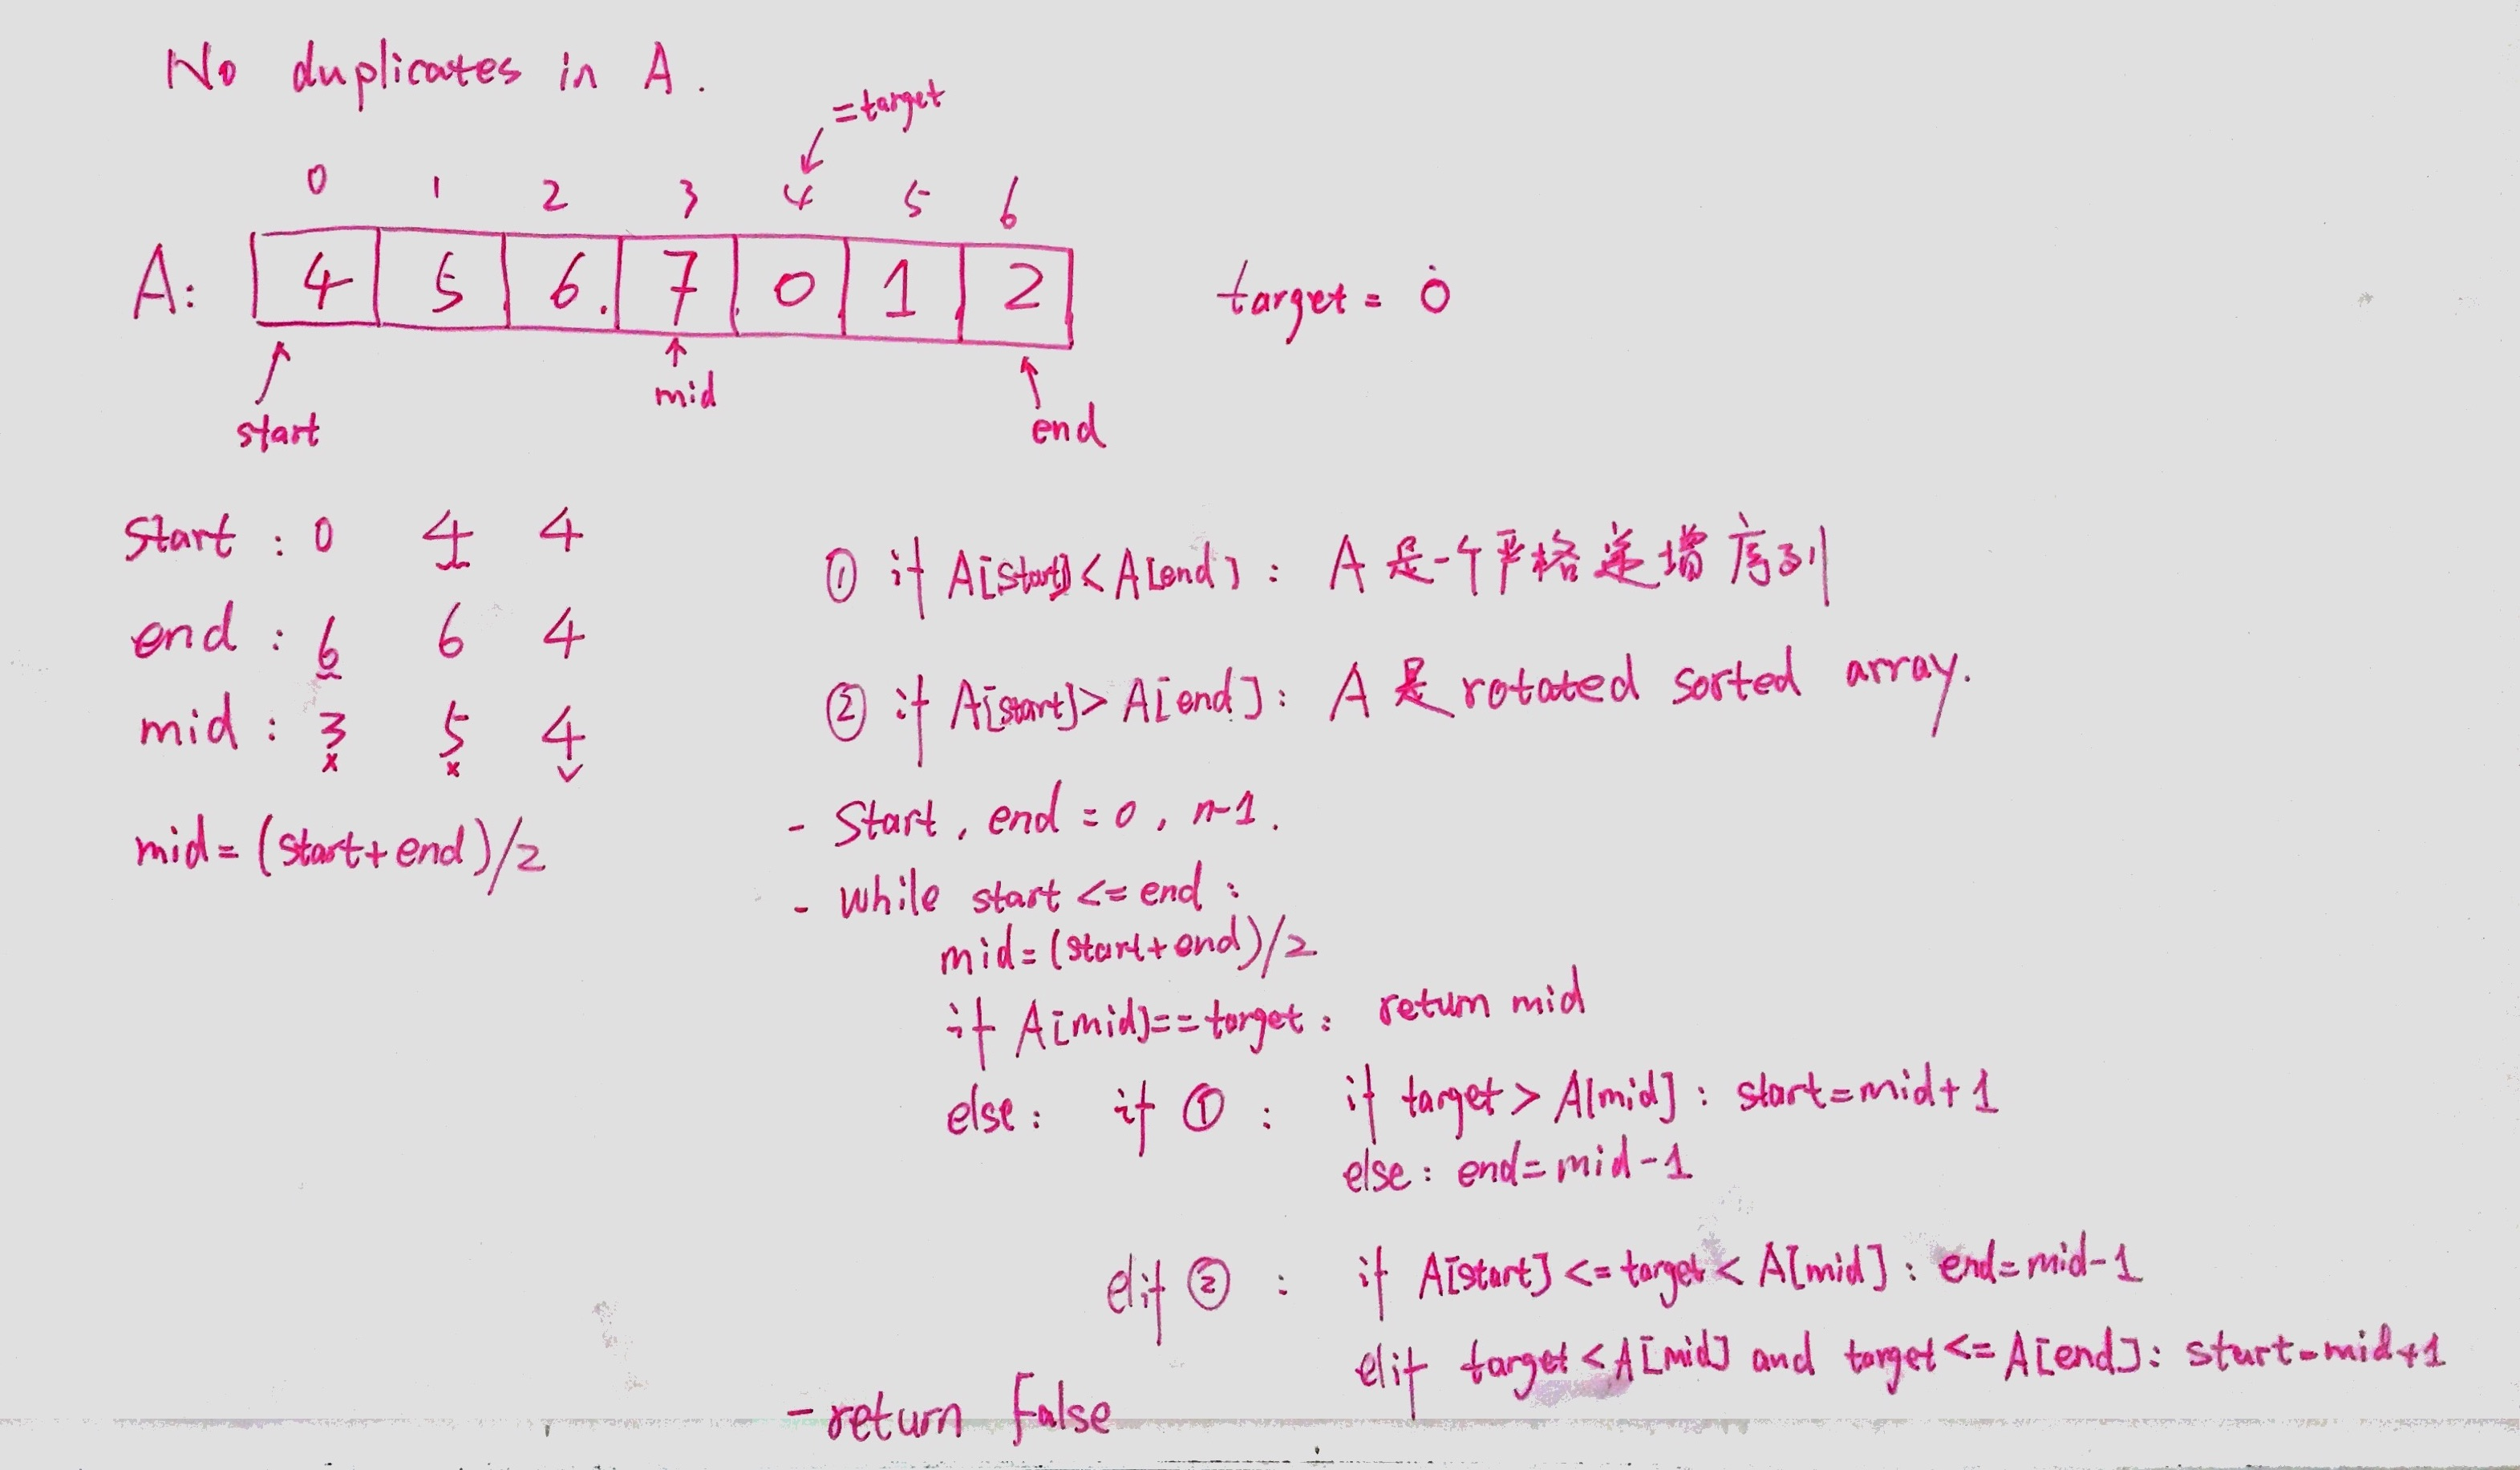
\includegraphics[width=\textwidth]{leetcode33.jpg}
    \centering \\
\end{figure}




\subsubsection{leetcode 81. Search in Rotated Sorted Array II}
Follow up for "Search in Rotated Sorted Array":
What if duplicates are allowed? Would this affect the run-time complexity? How and why? Write a function to determine if a given target is in the array.\\

\begin{CJK*}{UTF8}{gbsn}
\noindent 解题思路:这道题是在leetcode 33 Search in Rotated Sorted Array基础上改编而来的。不同之处在于允许存在重复元素,这点不影响leetcode33中设计的二叉搜索算法框架,但是需要增加一个内层循环去除在边界上的重复元素,以便定位下一轮搜索的起止位置。在最坏情况下,即数组中的元素都是相同的,那么这个二叉的搜索算法的时间复杂度将增大到$O(n)$。参见下图示例。这里给出的代码进一步简化了程序的写法,但是背后原理是相同的。
\end{CJK*}

\begin{figure}[h]
    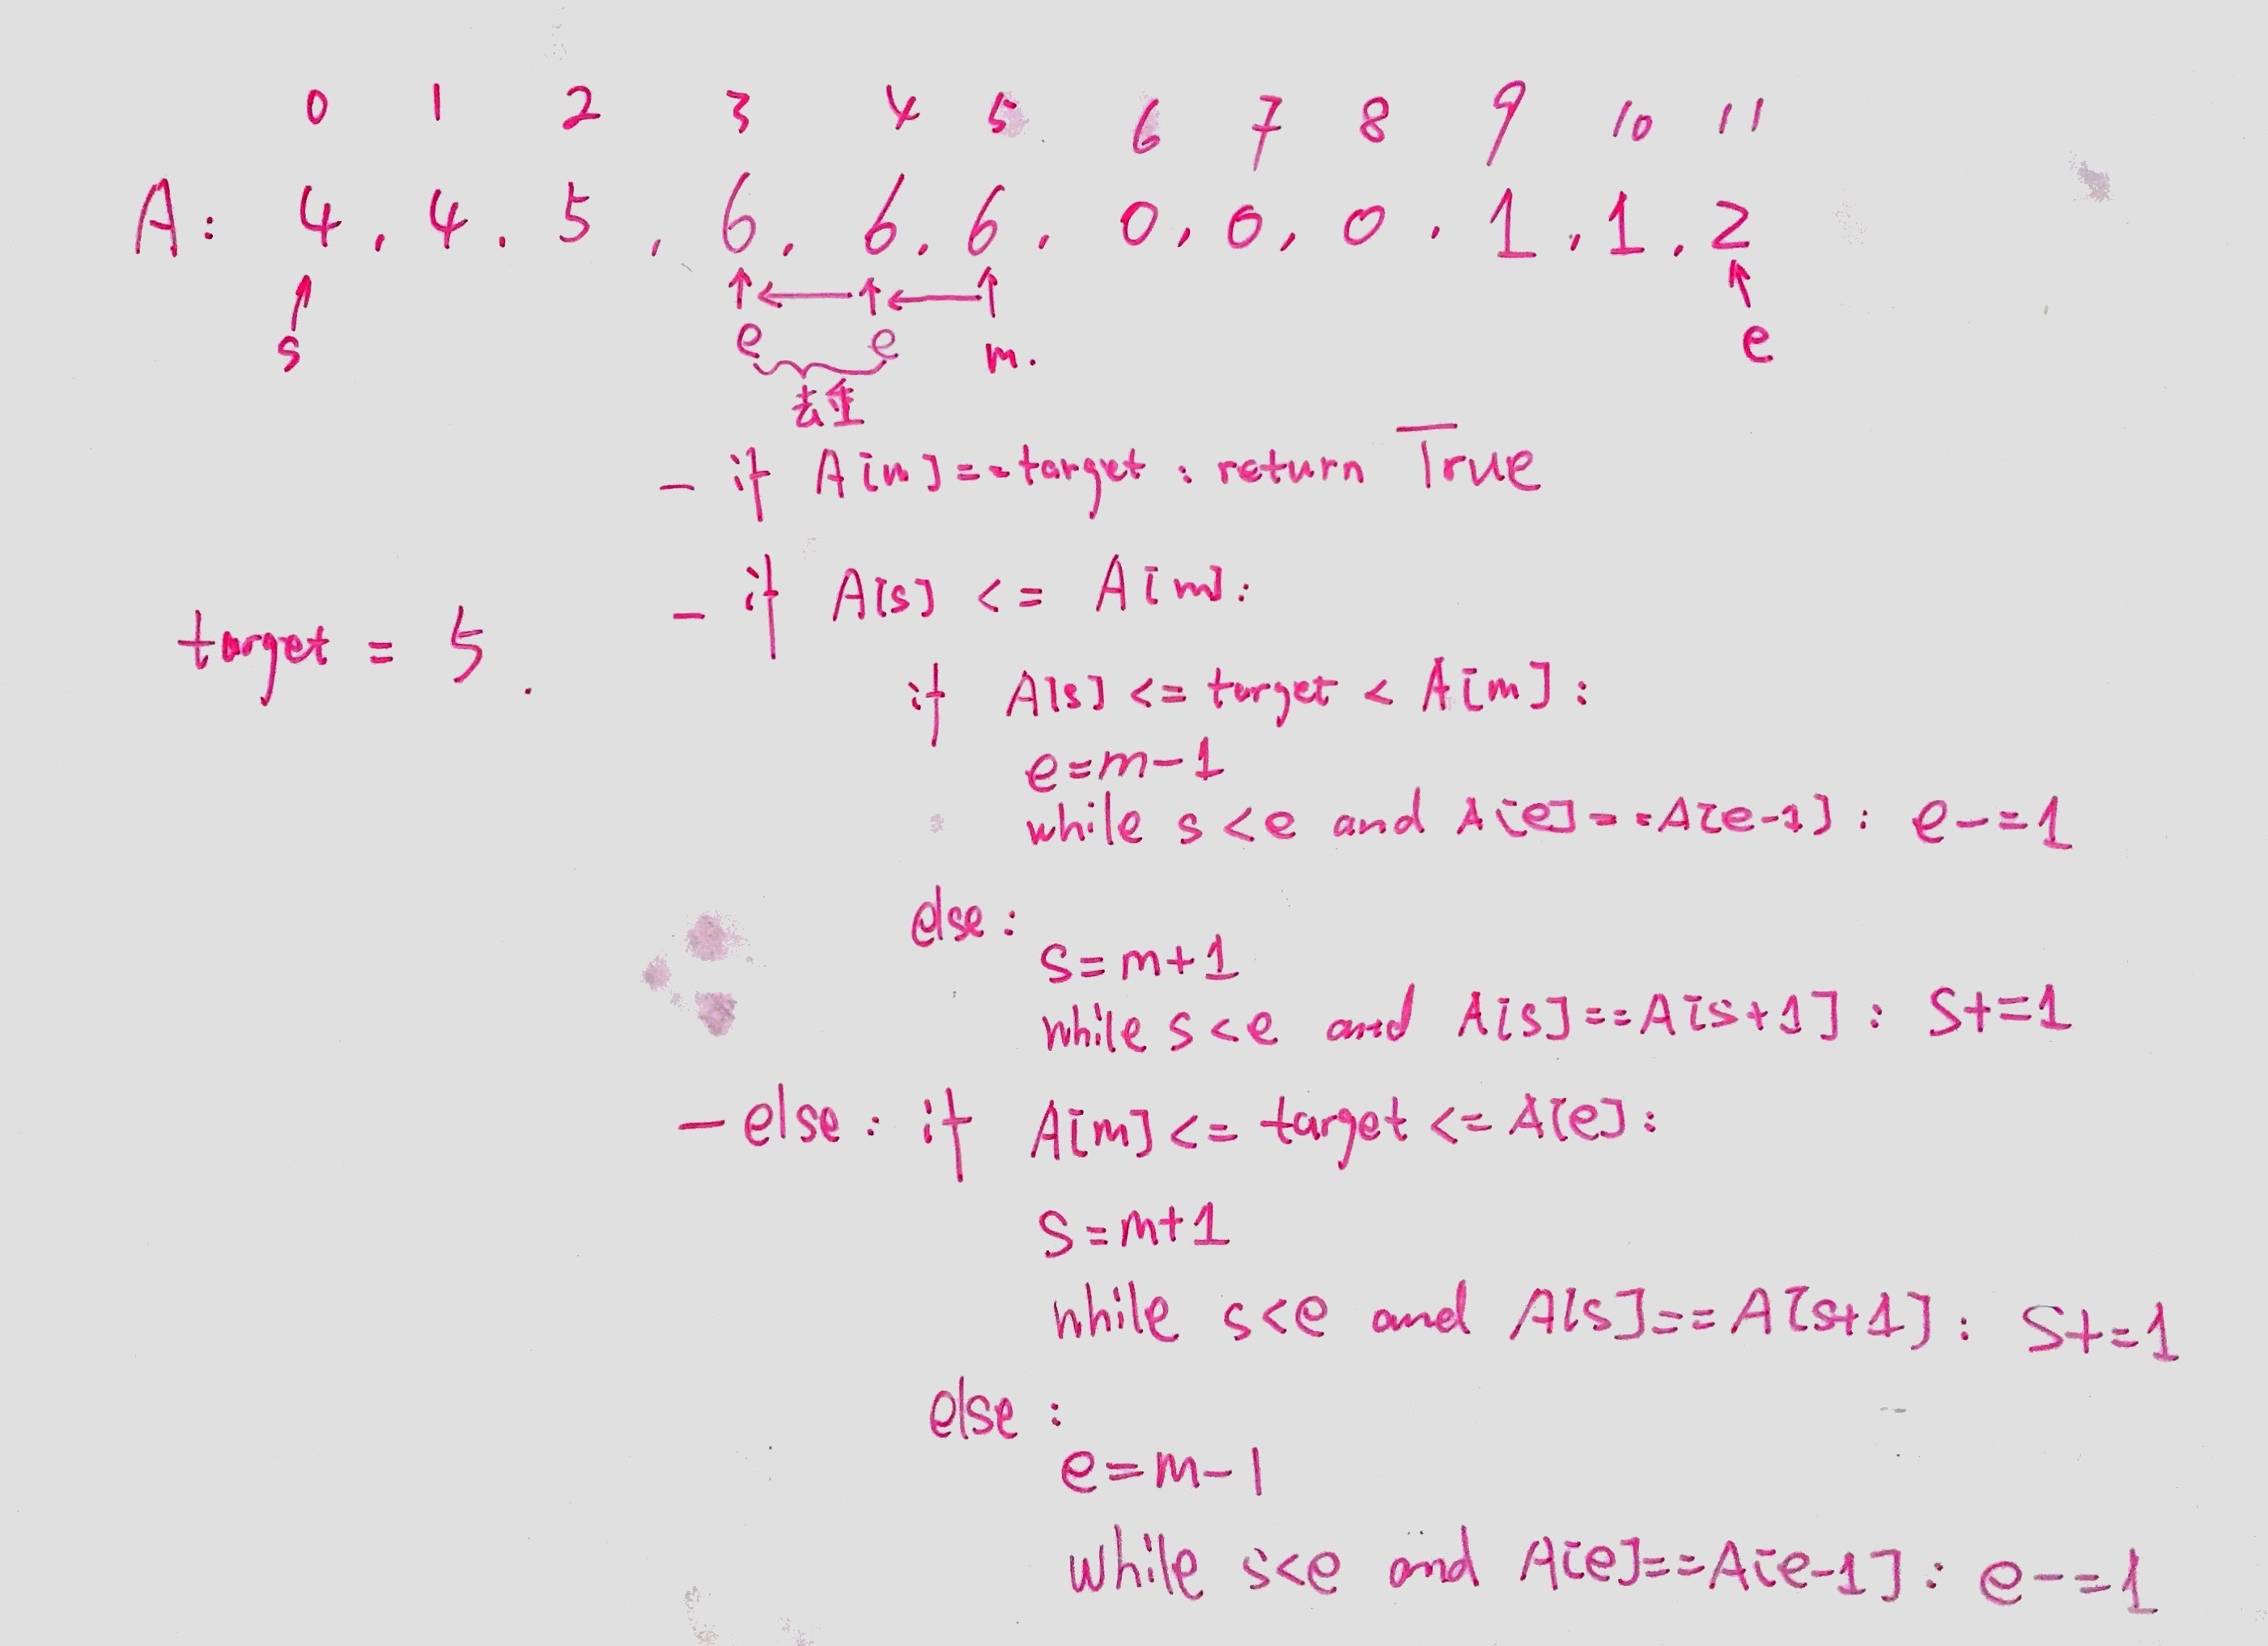
\includegraphics[width=\textwidth]{leetcode81.jpg}
    \centering
\end{figure}

\begin{lstlisting}[language=Python, caption=Problem81. Search in Rotated Sorted Array II]

class Solution(object):
    def search(self, nums, target): # RT: O(n), space: O(1)
        """
        :type nums: List[int]
        :type target: int
        :rtype: bool
        """
        first, last = 0, len(nums)-1
        while first <= last:
            mid = (first+last)/2
            if nums[mid] == target: return True
            if nums[first] < nums[mid]:
                if nums[first]<=target<=nums[mid]:
                    last = mid
                else:
                    first = mid + 1
            elif nums[first] > nums[mid]:
                if nums[mid]<=target<=nums[last]:
                    first = mid + 1
                else:
                    last = mid
            else:
                first += 1 # deal with duplicates
                
        return False
\end{lstlisting}


\subsubsection{leetcode 4. Median of Two Sorted Arrays}

There are two sorted arrays nums1 and nums2 of size $m$ and $n$ respectively. Find the median of the two sorted arrays. The overall run time complexity should be $O(\log (m+n))$.\\

\begin{CJK*}{UTF8}{gbsn}
\noindent 解题思路:这道题要求返回两个已经排好序的数列的中位数。中位数的定义:如果数列有偶数个数值,那么中位数为中间两个数的平均值;如果数列有奇数个数,那么中位数为中间的那个数。比如\{1,2,3,4,5\}的中位数为3。\{1,2,3,4,5,6\}的中位数为$(3+4)/2 = 3.5$。\\

\noindent这题最直接的思路就是将两个数列合并在一起,然后排序,然后找到中位数就行了。可是这样最快也要O((m+n)log(m+n))的时间复杂度,而题目要求O(log(m+n))的时间复杂度。那么,这道题其实考察的就是binary search,即如何设计二叉搜索算法找到两个数列中第$k=(m+n)/2$个小的元素(对于偶数数列的情况,就是用同样的方法找到中间两个数。)\\

\noindent参考下图中的示例,我们假设数组$A$总是比较短的那个数组。我们想找到两个有序数组中第$k=7$个小的元素呢?利用二分查找的思想,在数组$A$中取前$k/2=3$个元素$[1,3,5]$,在数组$B$中取前$k-3=4$个元素$[2,4,6,8]$,然后我们比较这两个数列中各自最后一个数值的大小,因为$5<8$,那么就暗示了从$A$中取出的这个数列$[1,3,5]$的任何一个元素一定都不是第7个数,那么我们就可以将这3个数从数组$A$的候选元素中去掉;与此同时,因为去掉了三个数,那么$k$也要减去相应的数值,即我们现在只需要在剩余的两个有序序列中找到第$k=7-3=4$个小的数值。以此类推,直到$k=1$时,再次比较两个数组相应的值,小的一个即为第$k$个小的元素。从上面的描述,我们可以发现这是一个递归的过程,而$k=1$就是递归定义中的base case。
\end{CJK*}

\begin{figure}[h]
    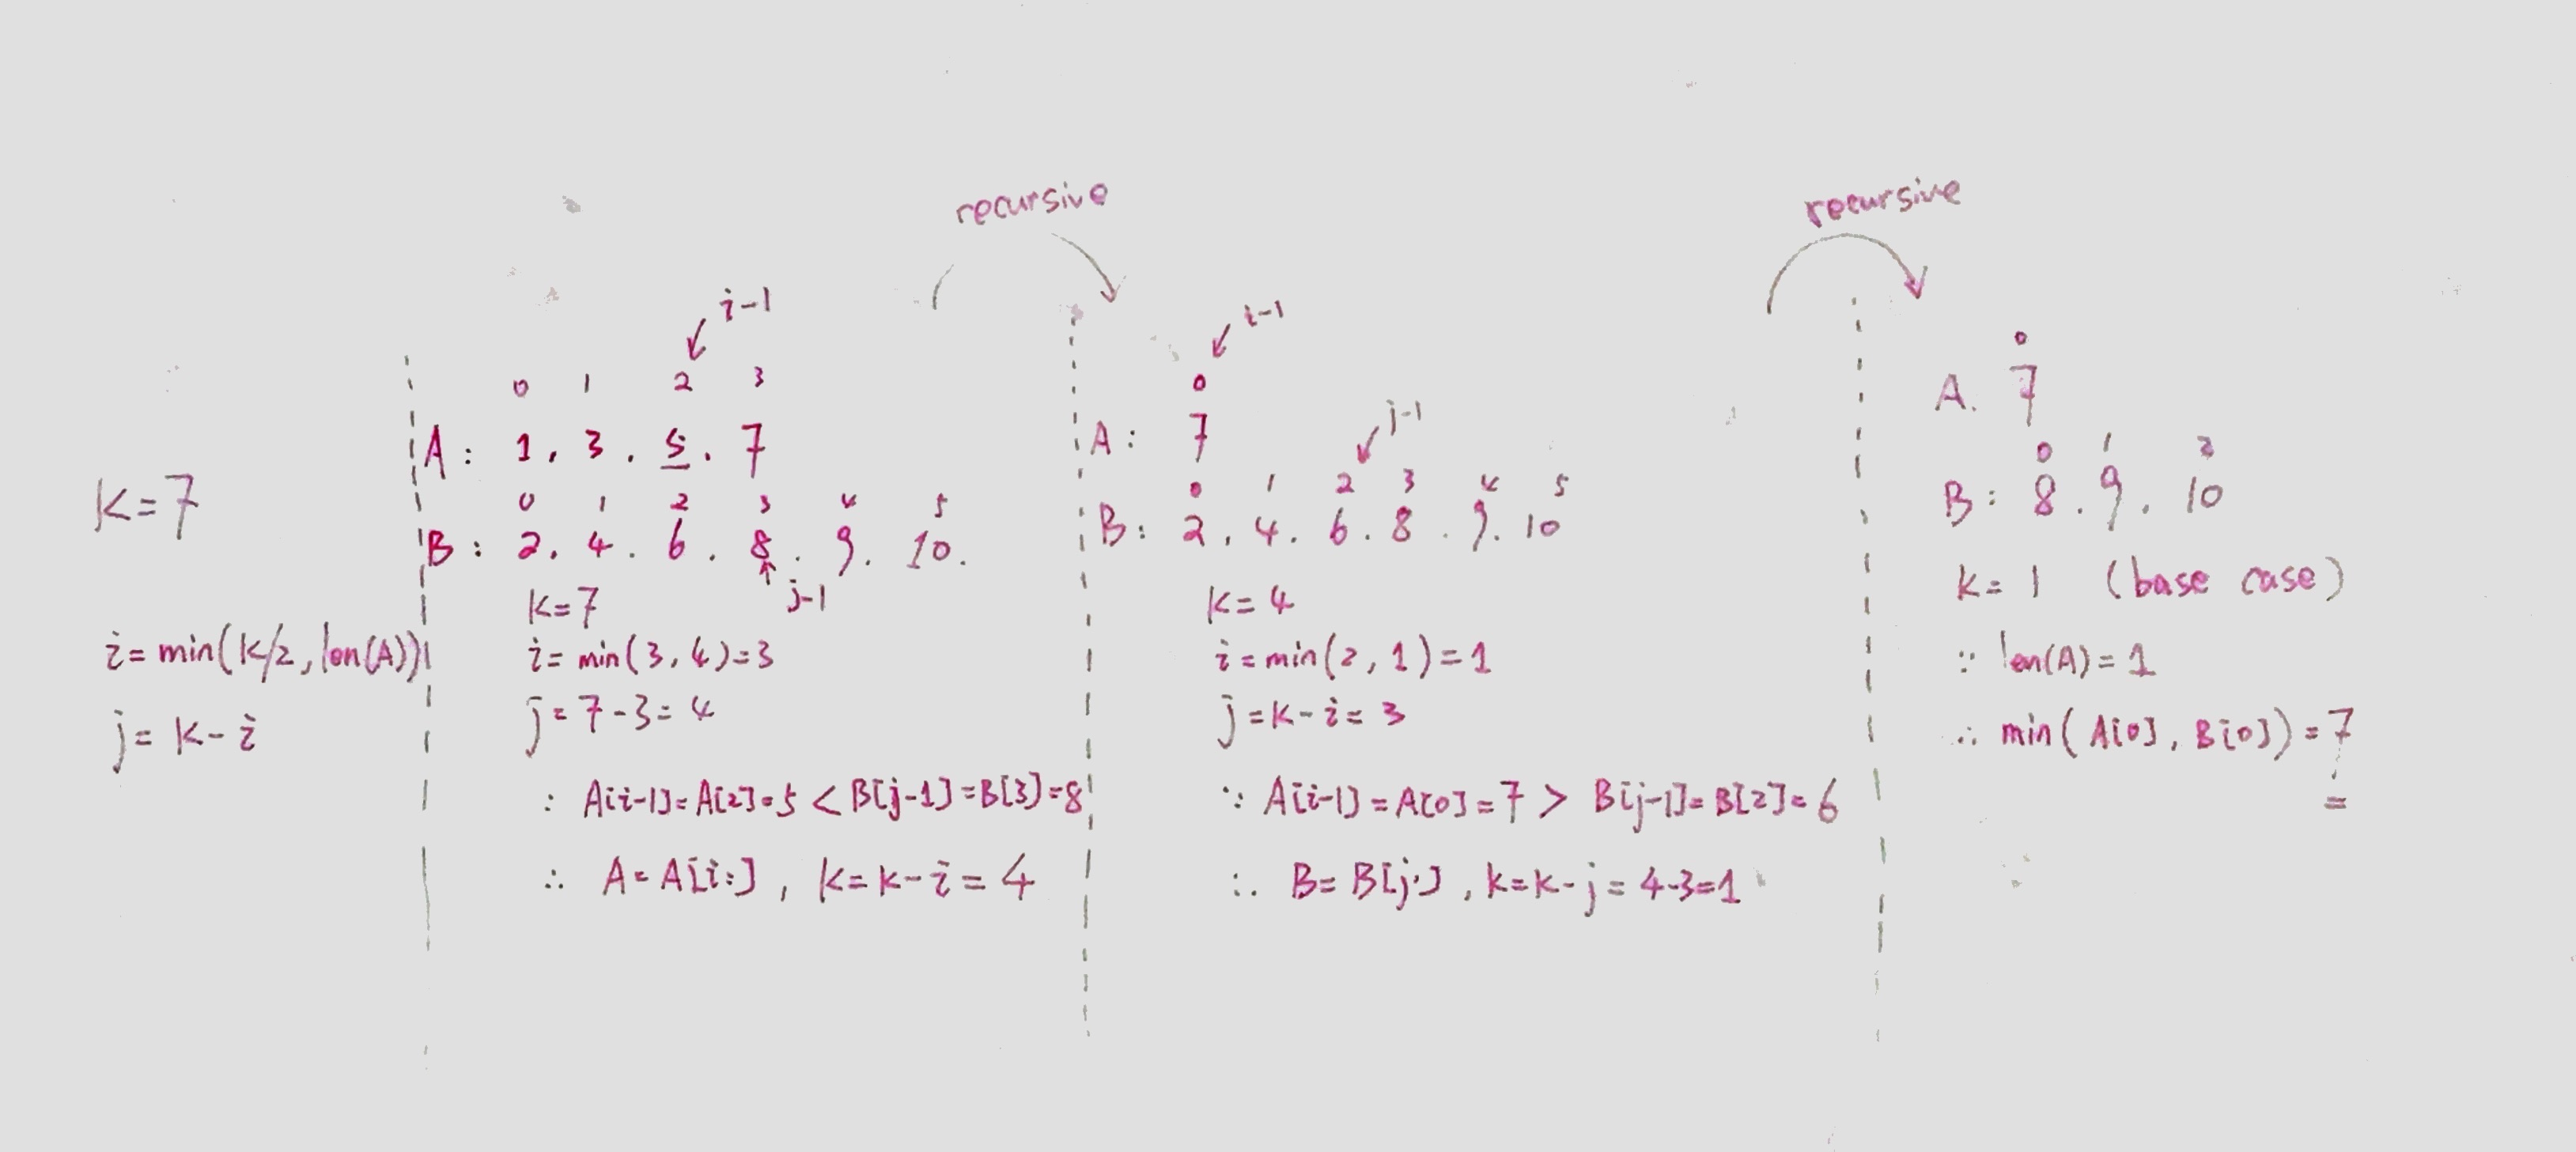
\includegraphics[width=\textwidth]{leetcode4.jpg}
    \centering
\end{figure}

\begin{lstlisting}[language=Python, caption=Problem4. Median of Two Sorted Arrays]

class Solution(object):
    # use binary search idea: each time removes k/2 elements at most
    # RT: O(log(m+n)), m is the length of nums, n is the 
    # length of nums2
    def findMedianSortedArrays(self, nums1, nums2): 
        """
        :type nums1: List[int]
        :type nums2: List[int]
        :rtype: float
        """
        total = len(nums1) + len(nums2)
        if total % 2 != 0:  # total is odd
            return self.find_kth(nums1, nums2, total/2+1)
        else:
            return (self.find_kth(nums1, nums2, total/2) + self.find_kth(nums1, nums2, total/2+1)) / 2.0
        
    def find_kth(self, nums1, nums2, k):
        # always assume the length of nums1 is less than that of nums2
        if len(nums1) > len(nums2):
            return self.find_kth(nums2, nums1, k)
        
        if len(nums1) == 0:
            return nums2[k-1]
        if k == 1:
            return min(nums1[0], nums2[0])
        
        n1 = min(k/2, len(nums1))
        n2 = k - n1
        if nums1[n1-1] < nums2[n2-1]:
            return self.find_kth(nums1[n1:], nums2, k-n1)
        elif nums1[n1-1] > nums2[n2-1]:
            return self.find_kth(nums1, nums2[n2:], k-n2)
        else:
            return nums1[n1-1]
\end{lstlisting}



\subsubsection{leetcode 128. Longest Consecutive Sequence}
Given an unsorted array of integers, find the length of the longest consecutive elements sequence. For example, Given [100, 4, 200, 1, 3, 2], The longest consecutive elements sequence is [1, 2, 3, 4]. Return its length: 4. Your algorithm should run in O(n) complexity.\\

\begin{CJK*}{UTF8}{gbsn}
\noindent 解题思路:因为题目中已经指出数组是无序的,所以最直接的想法就是先排序,然后再遍历数组,得出最后的结果。这个思路设计出来的算法,时间复杂度是$O(nlogn)$。而题目要求的时间复杂度是$O(n)$。在$O(n)$时间内对无序的数组完成某种需要遍历才能完成的任务时通常就是考虑使用hashtable(在Python里面就用字典)。
\end{CJK*}

\begin{lstlisting}[language=Python, caption=Problem128. Longest Consecutive Sequence]

class Solution(object):
    def longestConsecutive(self, nums):
        """
        :type nums: List[int]
        :rtype: int
        """
        if len(nums) <= 1:
            return len(nums)
        
        # Because the time complexity is O(n), have to 
        # use an dictionary or hashmap. 
        # If the time complexity is O(nlog(n)), 
        # we can sort nums first.
        dict = {}   
        for i in nums:
            dict[i] = False
        
        longest = 0
        for i in nums:
            if dict[i] == True:
                 continue
            length = 1
            dict[i] = True
            
            # check the consecutivity of the right 
            # side of the current key
            j = i+1
            while dict.has_key(j):
                dict[j] = True
                length += 1
                j += 1
            
            # check the consecutivity of the left 
            # side of the current key
            j = i-1
            while dict.has_key(j):
                dict[j] = True
                length += 1
                j -= 1
            
            # check the longest length
            longest = max(longest, length)
            if longest == len(nums): break
        
        return longest
\end{lstlisting}


\subsubsection{leetcode 1. TwoSum}
Given an array of integers, find two numbers such that they add up to a specific target number. The function twoSum should return indices of the two numbers such that they add up to the target, where index1 must be less than index2. Please note that your returned answers (both index1 and index2) are not zero-based. \\

\noindent You may assume that each input would have exactly one solution.
\begin{itemize}
    \item Input: numbers=$\{2, 7, 11, 15\}$, target=9
    \item Output: index1=1, index2=2
\end{itemize}

\begin{CJK*}{UTF8}{gbsn}
\noindent 解题思路:这道题最直接的思路就是暴力遍历所有组合方式,时间复杂度就是$O(n^2)$。但是,显然这不是考点。题目的重点应该是数据结构对算法设计的影响。暴力组合的方法存在的问题是每次选择一个元素后,就需要验证数组的其余元素是否能与这个元素加和后等于目标值,这是造成时间复杂度增高的原因,如果可以在常数时间内完成验证就可以有效降低算法的时间复杂度。那么可以完成$O(1)$查找的数据结构就是哈希表或者字典。两种方法的示例见下图。另外,需要注意的一点是题目中没有说数组是有序的,所以如果用暴力组合的方法,先进行排序会让代码更简洁些。\\
\end{CJK*}

\begin{lstlisting}[language=Python, caption=Problem1. TwoSum]

class Solution:
    # @return a tuple, (index1, index2)
    def twoSum(self, num, target):
        # use an dictionary to implement, 
        # but there are no dulicates in num. 
        # RT is O(n).
        dict = {}
        for i in range(len(num)):
            x = num[i]
            if target - x in dict:
                return dict[target-x], i
            dict[x] = i
        return -1, -1
        
    def twoSum_bruteforce(self, num, target):
        # brute force method: Use list to implement.
        # RT: O(n^2).
        if len(num) <= 1:
            return -1, -1

        list = []
        for i in range(len(num)):
            list.append((i, num[i]))

        list.sort(key=lambda x: x[1])

        for i in range(len(list)):
            a = list[i][1]
            b = target - a

            if i+1 < len(list):
                for j in xrange(i+1, len(list)):
                    if b == list[j][1]:
                        if list[i][0] <= list[j][0]:
                            return list[i][0], list[j][0]
                        else:
                            return list[j][0], list[i][0]
        return -1, -1
\end{lstlisting}

\begin{figure}[h]
    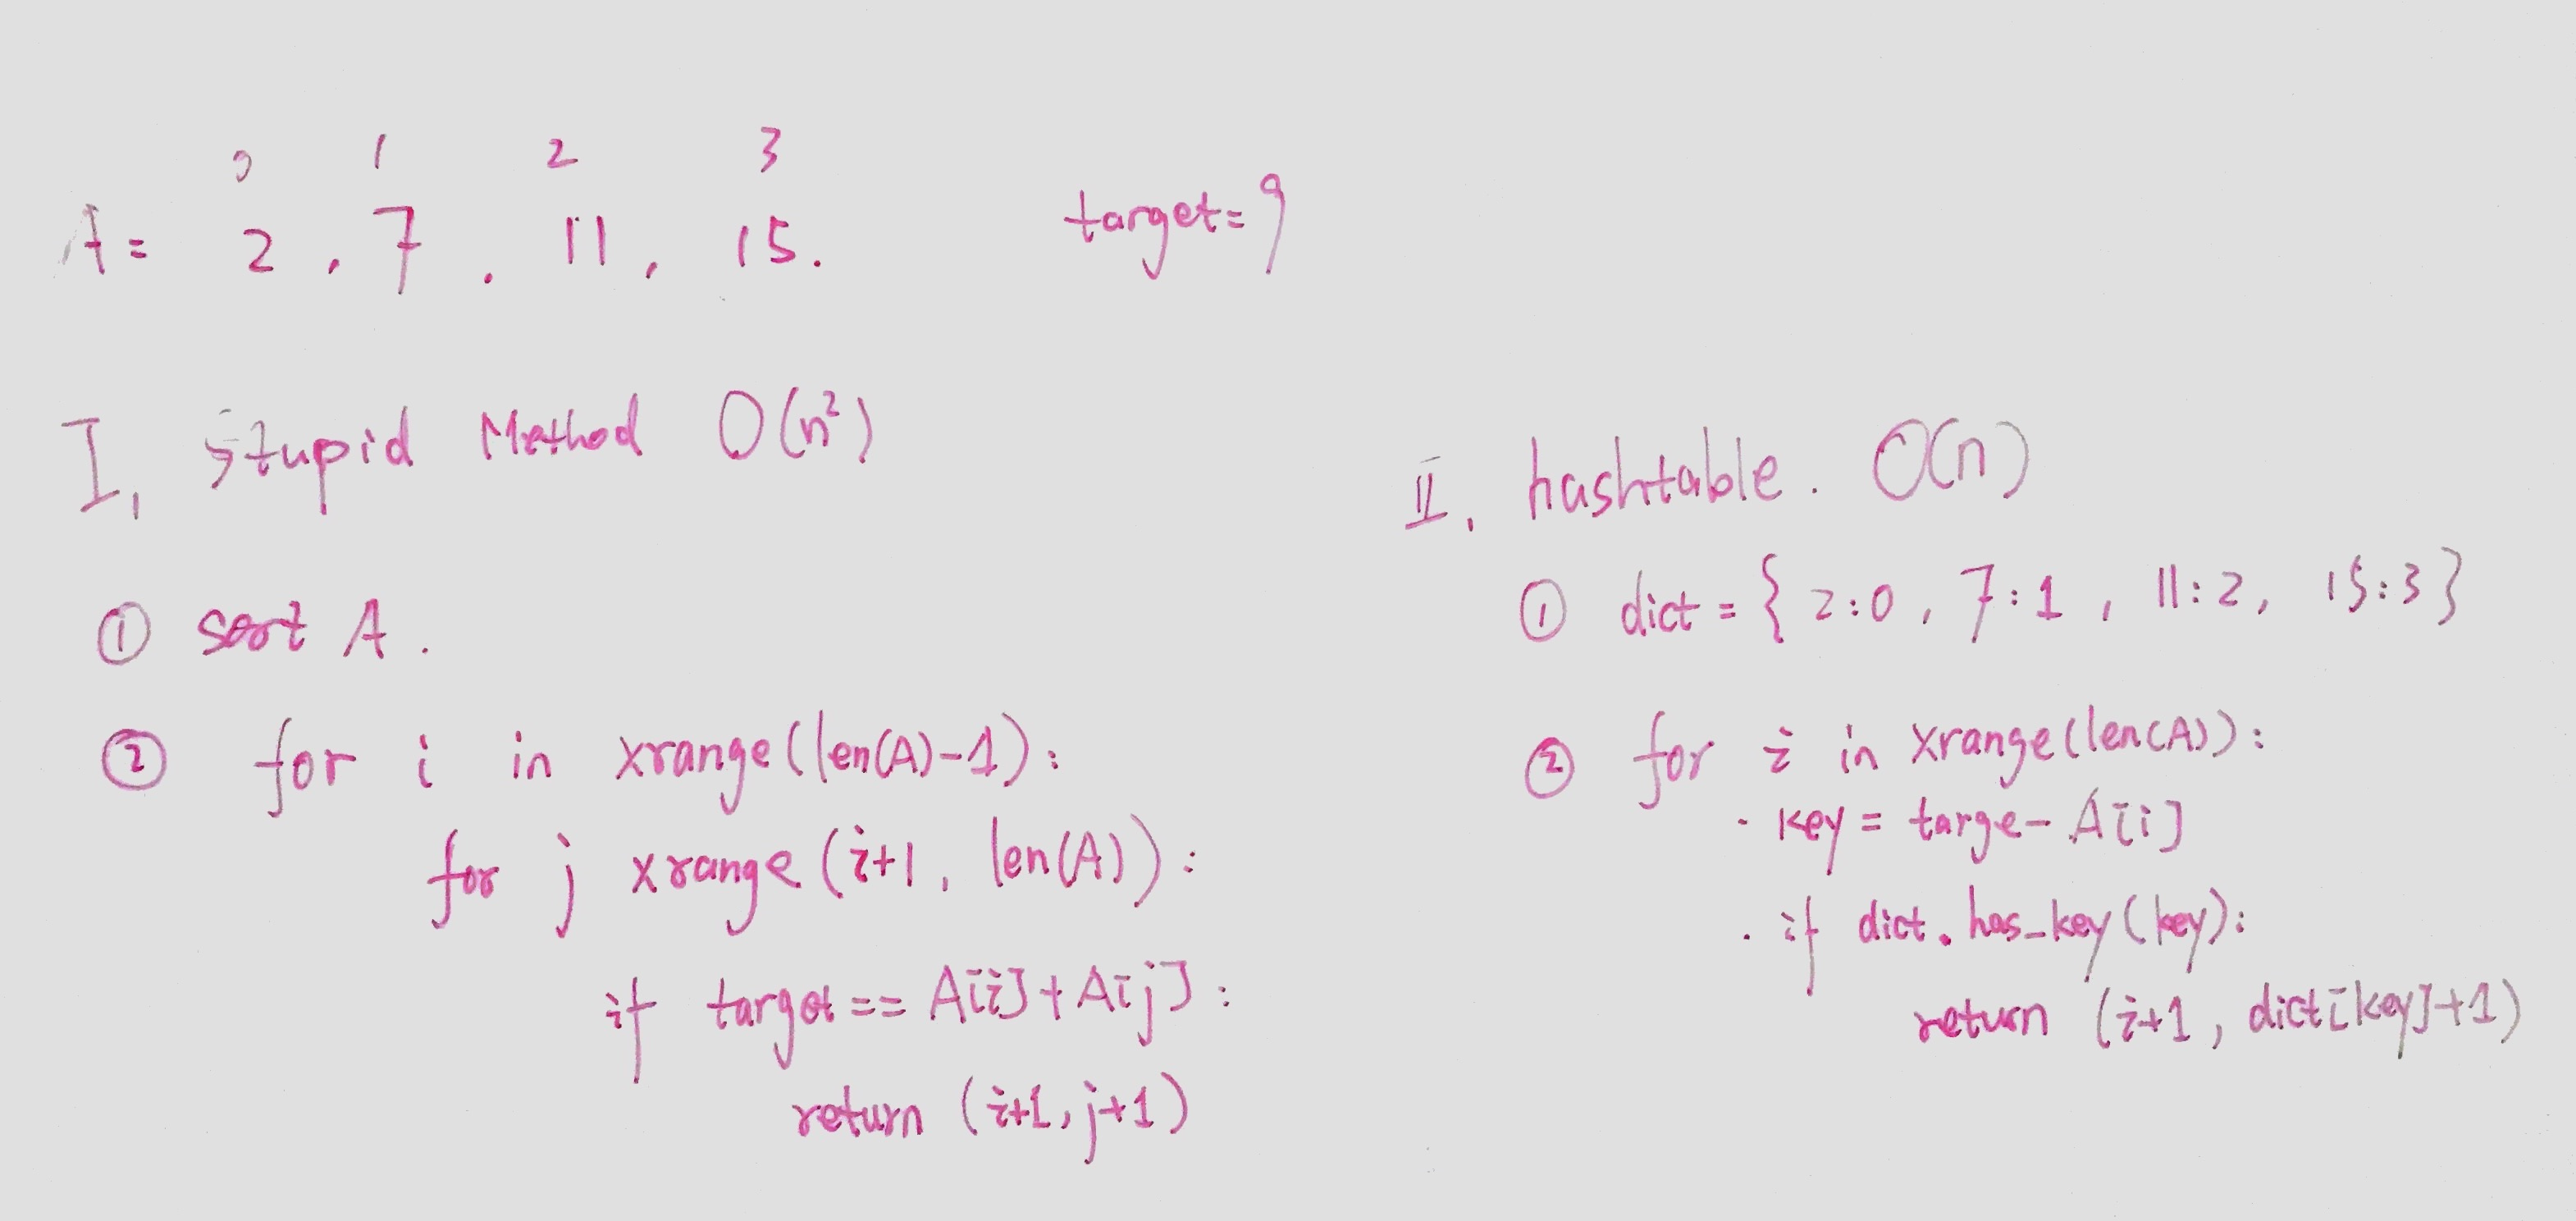
\includegraphics[width=\textwidth]{leetcode1.jpg}
    \centering \\
\end{figure}


\subsubsection{leetcode 15. 3Sum}
Given an array S of n integers, are there elements a, b, c in S such that a + b + c = 0? Find all unique triplets in the array which gives the sum of zero. Note:
\begin{itemize}
    \item Elements in a triplet (a,b,c) must be in non-descending order. (ie, $a\leq b\leq c$)
    \item The solution set must not contain duplicate triplets.
\end{itemize}

\noindent For example, given array $S = \{-1,0,1,2,-1,-4\}$, A solution set is: $(-1, 0, 1)$, $(-1, -1, 2)$. \\
    
\begin{CJK*}{UTF8}{gbsn}
\noindent 解题思路:题目要求输出实际的组合值,所以最直接的想法就是DFS遍历决策树。为了达到结果中没有重复组合,需要排序,并且存储过程结果数据结构用集合set。但是,这样设计的算法在OJ的测试过程中超时。第二种算法思想和DFS类似,但是更为通用,可以计算任意一种$k$个数字累加和等于指定值的情况。
\end{CJK*}

\begin{lstlisting}[language=Python, caption=Problem15. 3Sum]

class Solution(object):
    def threeSum_dfs(self, nums): # DFS, but TLE
        """
        :type nums: List[int]
        :rtype: List[List[int]]
        """
        def dfs(depth, target, nums, valuelist):
            if depth == 0:
                if target == 0: res.add(tuple(valuelist))
                return
            if target<nums[0] or target>nums[len(nums)-1]: return
            for i in xrange(len(nums)-depth+1):
                dfs(depth - 1, target - nums[i], nums[i + 1:], valuelist + [nums[i]])
        if nums==[]: return []
        nums.sort()
        res = set()
        dfs(3, 0, nums, [])
        return [list(t) for t in res]
        
    def threeSum_Generic(self, nums):
        """
        :type nums: List[int]
        :rtype: List[List[int]]
        """
        def ksum(nums,k,target):
            # This is a generic k-sum algorithm
            res = set() # avoid duplicates
            i=0
            if k==2:
                j = len(nums)-1
                while i<j:
                    if nums[i]+nums[j]==target:
                        res.add((nums[i],nums[j]))
                        i+=1
                    elif nums[i]+nums[j]>target:
                        j-=1
                    else:
                        i+=1
            else:   # case: k>2
                for i in xrange(len(nums)-k+1):
                    newtarget = target - nums[i]
                    subresult = ksum(nums[i+1:], k-1, newtarget)
                    if subresult:
                        res |= set((nums[i],)+nr for nr in subresult)
            return res
        
        nums.sort() # O(nlog(n))
        return [list(t) for t in ksum(nums, 3, 0)]
\end{lstlisting}

\subsubsection{leetcode 16. 3Sum Closest}
Given an array $S$ of $n$ integers, find three integers in S such that the sum is closest to a given number, target. Return the sum of the three integers. You may assume that each input would have exactly one solution. \\

\noindent For example, given array $S = \{-1,2,1,-4\}$, and target = 1.
The sum that is closest to the target is 2. $(-1 + 2 + 1 = 2)$. \\

\begin{CJK*}{UTF8}{gbsn}
\noindent 解题思路:这道题是求所有三个数的组合中,那个组合的累加和在数轴上最接近指定的目标值。构成三个数的组合的通常解法就是先在数组中任选一个数$i$,那么数组中剩下的数就构成了组合中另外两个数$j,k$的候选集合。如果这个数组是有序,那么$j$和$k$的初始位置就可以分别选在候选集合的两段:如果三者的和小于目标值,那么就可以根据数组是有序递增序列的性质,保持$k$不便,将$j$向高位移动;如果三者之和大于目标值,就将$k$向低位移动;如果三者之和等于目标值,那就直接返回结果,程序结束。参考下图中的示例。\\
\end{CJK*}


\begin{lstlisting}[language=Python, caption=Problem16. 3Sum Closest]

class Solution(object):
    def threeSumClosest(self, nums, target): # O(n^2) time
        """
        :type nums: List[int]
        :type target: int
        :rtype: int
        """
        nums.sort()     # O(nlog(n))
        import sys
        min_gap = sys.maxint
        res = 0

        for i in range(len(nums)-3+1):  # O(n^2)
            j = i+1
            k = len(nums)-1
            while j < k:
                sum = nums[i]+nums[j]+nums[k]
                gap = abs(target-sum)
                if gap < min_gap:
                    min_gap = gap
                    res = sum
                    if min_gap == 0:
                        return target
                if sum < target: j += 1
                else: k -= 1
        return res
\end{lstlisting}

\begin{figure}[h]
    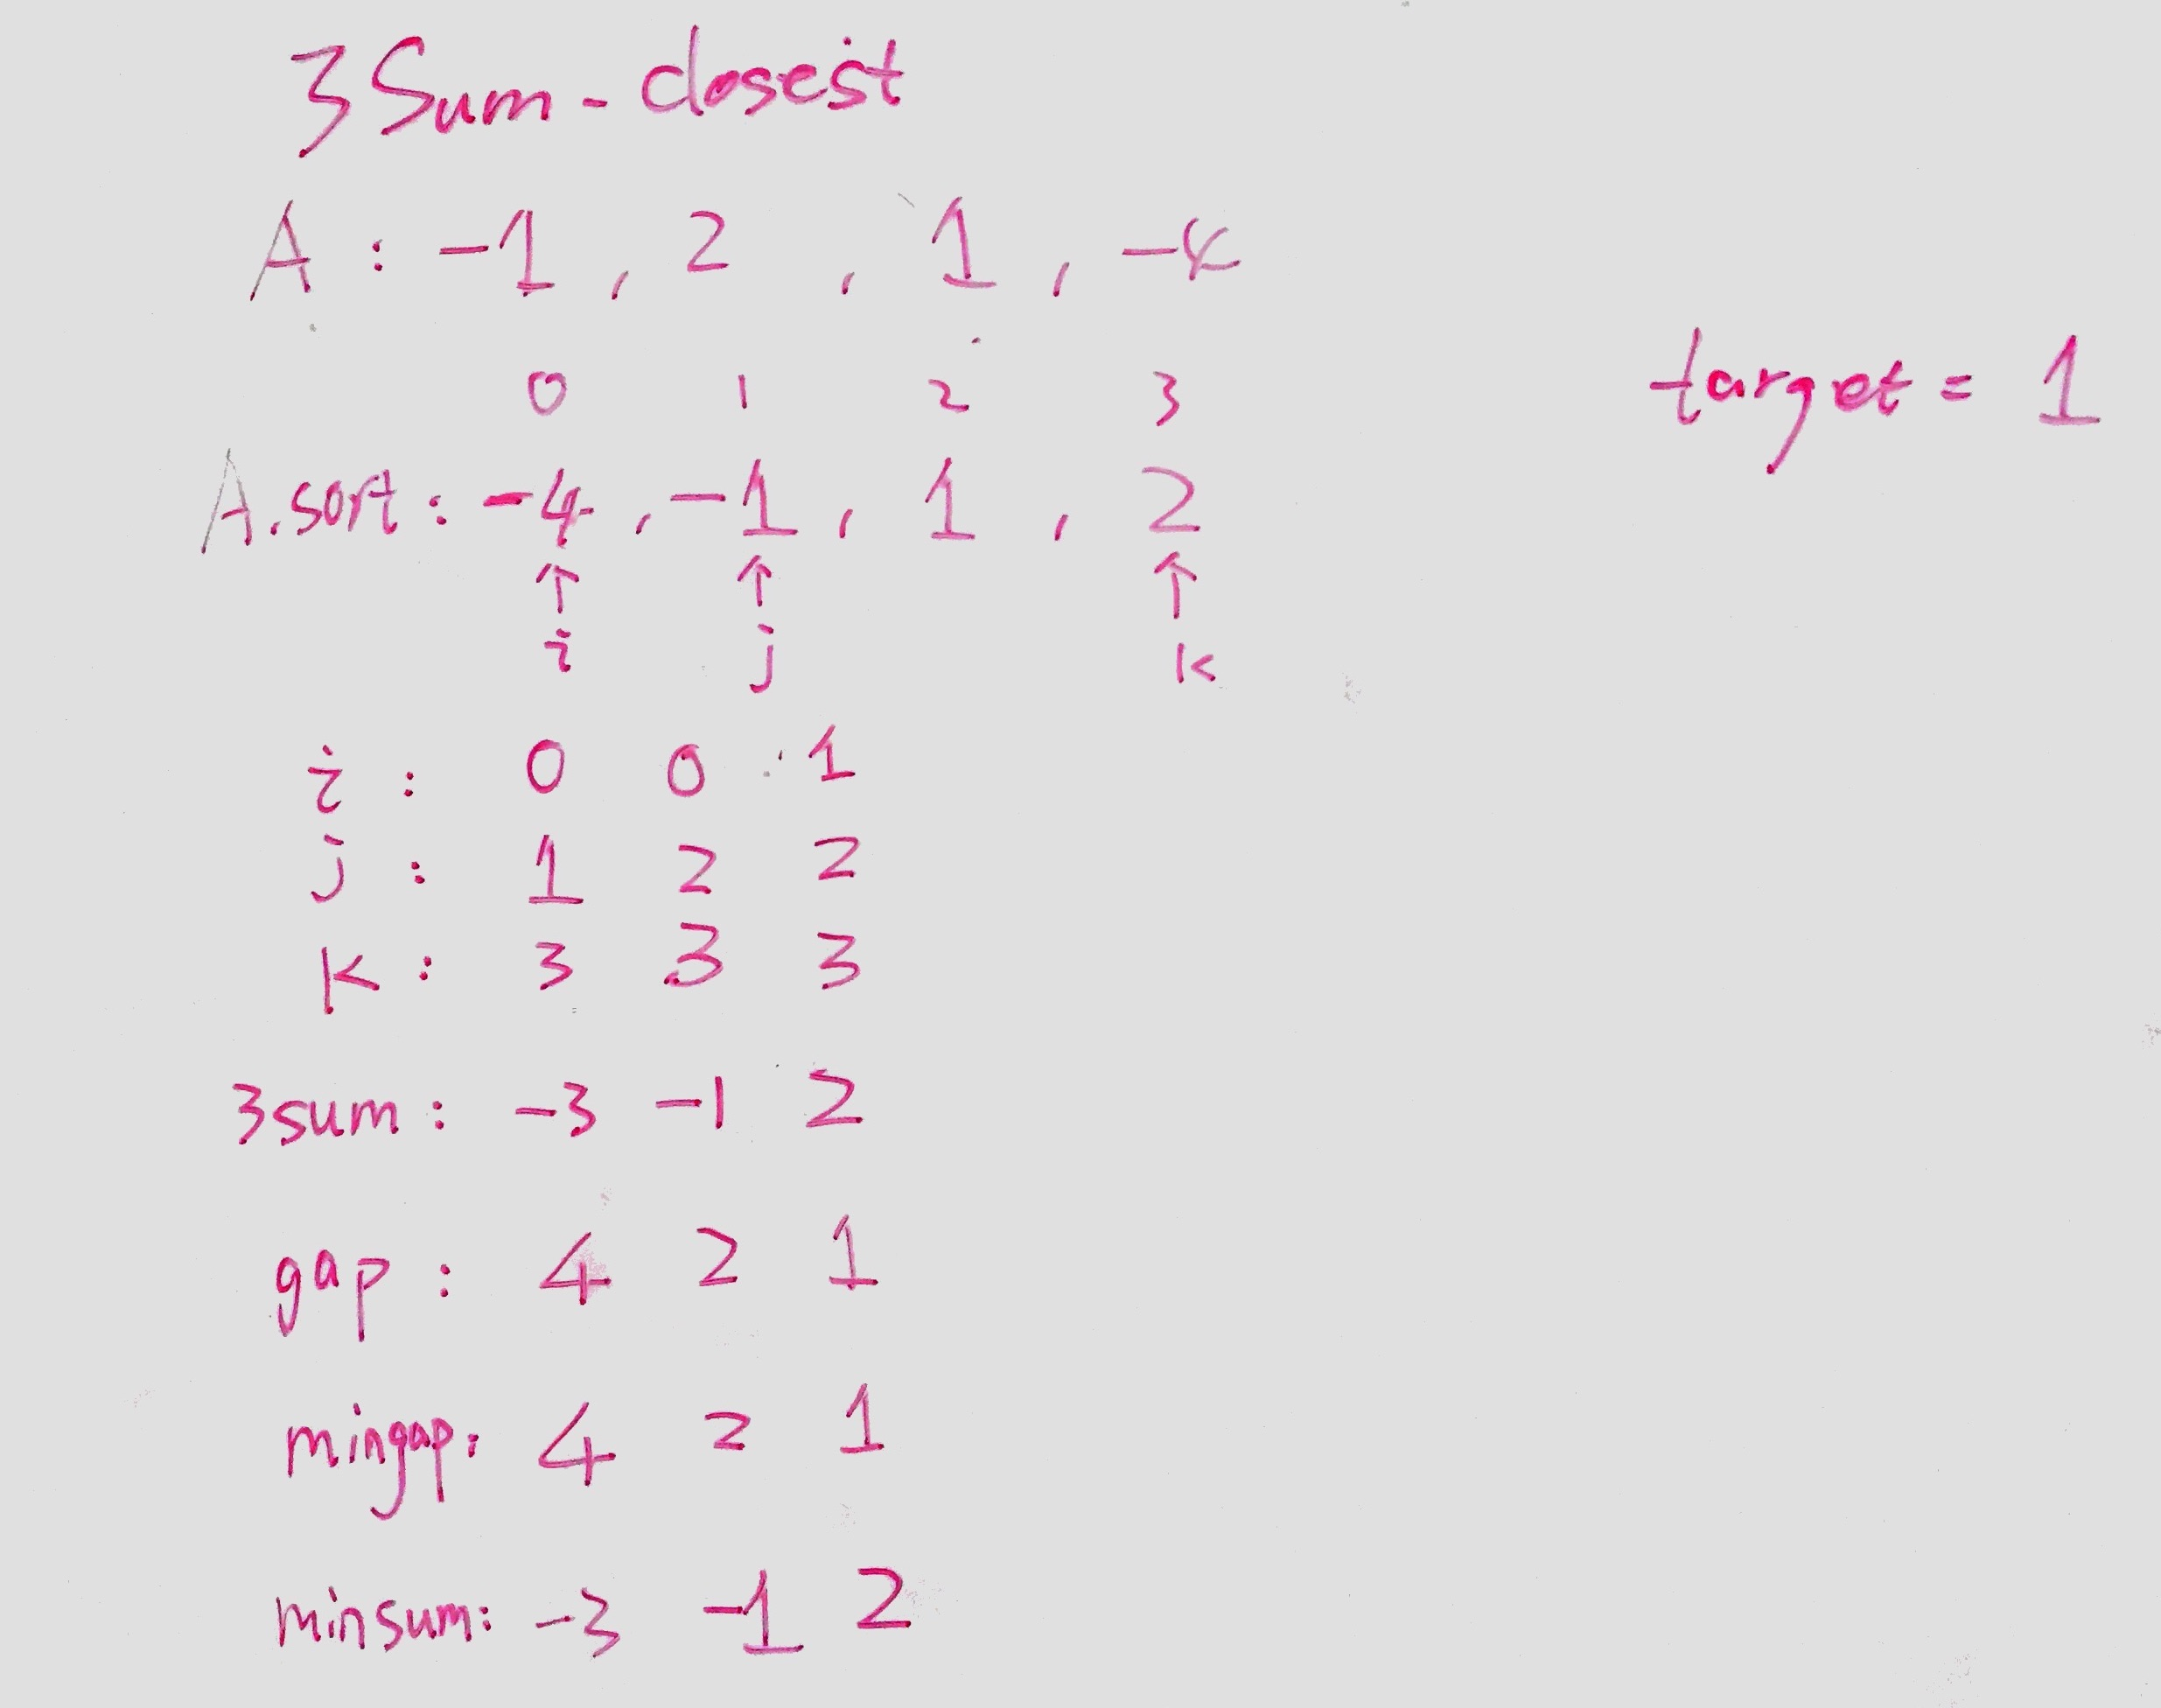
\includegraphics[width=\textwidth]{leetcode16.jpg}
    \centering \\
\end{figure}



\subsubsection{leetcode 18. 4Sum}
Given an array S of n integers, are there elements a, b, c, and d in S such that a + b + c + d = target? Find all unique quadruplets in the array which gives the sum of target. Note:
\begin{itemize}
    \item Elements in a quadruplet (a,b,c,d) must be in non-descending order. (ie, $a \leq b \leq c \leq d$)
    \item The solution set must not contain duplicate quadruplets.
\end{itemize}

\noindent For example, given array $S = \{1,0,-1,0,-2,2\}$, and target = 0.
    A solution set is:
    $(-1,  0, 0, 1)$
    $(-2, -1, 1, 2)$
    $(-2,  0, 0, 2)$ \\

\begin{CJK*}{UTF8}{gbsn}
\noindent 解题思路:这道题可以设计三种算法解题:DFS遍历决策树,ksum通用算法,以及利用hashtable的算法。前两种无需开辟额外空间就可以解决问题,但是时间复杂度比较高,OJ上通不过。所以,也可以反应出这道题的考查点应该是第三种算法设计思路,即利用“空间换时间”的思路,选择合适的数据结构,降低算法时间复杂度。
\noindent 在Python中,可以通过字典dict来模拟hashtable:字典的key值为数组中每两个元素的和,每个key对应的value为这两个元素的下标组成的元组,元组不一定是唯一的。如对于num=[1,2,3,2]来说,dict=\{3:[(0,1),(0,3)], 4:[(0,2),(1,3)], 5:[(1,2),(2,3)]\}。 这样就可以检查(target-key)的差值是不是dict的key值中,如果差值是dict中的一个key并且下标符合要求,那么就找到了这样的一组解。由于需要去重,这里选用set()类型的数据结构,即无序无重复元素集。最后将每个找出来的解(set()类型)转换成list类型输出即可。下面的代码给出了第二、三种算法的实现。\\
\end{CJK*}


\begin{lstlisting}[language=Python, caption=Problem18. 4Sum]

class Solution(object):
    def fourSum_hash(self, nums, target):    # time complexity is O(n^2)
        nums.sort()
        n = len(nums)
        res = set()
        dict = {}
        # establish the dict
        for i in xrange(n-1):
            for j in xrange(i+1, n):
                sum = nums[i]+nums[j]
                # there could be duplicates
                if dict.has_key(sum):
                    dict[sum].append((i,j))
                else:
                    dict[sum] = [(i,j)]
        for i in xrange(n-4+1):
            for j in xrange(i+1, n-4+2):
                newsum = target - nums[i] - nums[j]
                if dict.has_key(newsum):
                    for item in dict[newsum]:
                        # Elements in a quadruplet (a,b,c,d)
                        # must be in non-descending order
                        if j < item[0]:
                            res.add((nums[i],nums[j],nums[item[0]],nums[item[1]]))
        return [list(t) for t in res]

    # Generic algorithm, which has O(n^3) running time.
    def fourSum_Generic(self, nums, target): # Time Limit Exceeded
        """
        :type nums: List[int]
        :type target: int
        :rtype: List[List[int]]
        """
        def ksum(nums, k, target):
            result = set()
            i = 0
            
            if k==2:
                j=len(nums)-1
                while i<j:
                    if nums[i]+nums[j] == target:
                        result.add((nums[i],nums[j]))
                    elif nums[i]+nums[j] > target:
                        j-=1
                    else:
                        i+=1
            else:   # case: k>2
                while i < len(nums)-k+1:
                    newtarget = target - nums[i]
                    subresult = ksum(nums[i+1:], k-1, newtarget)
                    if subresult:
                        result = result | set((nums[i],)+nr for nr in subresult)
                    i+=1
            return result
        
        nums.sort()
        return [list(t) for t in ksum(nums, 4, target)]
\end{lstlisting}



\subsubsection{leetcode 27. Remove Element}
Given an \textbf{array} and a value, remove all instances of that value \textbf{in place} and return the new length. The \textbf{order} of elements can be \textbf{changed}. It doesn't matter what you leave beyond the new length.\\

\begin{CJK*}{UTF8}{gbsn}
\noindent 解题思路:这道题比较简单,这里给出下面两种思路:
\begin{itemize}
    \item 第一种解法是用两个指针$i$、$j$分别指向数组$A$的头和尾。
        \begin{enumerate}
            \item 移动指针$i$,直到A[i]==target,然后停止移动;
            \item 移动指针$j$,直到找到A[j]$\neq$target,然后将A[j]的值复制到A[i];
            \item 在i<j的情况下,继续移动指针$j$直到找到下一个A[j]$\neq$target。如果找到A[j],那么重复上述步骤;
            \item 最后,如果A[i]==target,则返回$i$;否则,返回$i+1$。
        \end{enumerate}
        
    \item 第二种解法是也是用两个指针$i$、$j$,但是同时指向数组$A$的开头。
        \begin{enumerate}
            \item 如果A[i]$\neq$target,将A[i]的值复制到A[j],然后同时移动指针$i$、$j$到下一个位置;
            \item 如果A[i]==target,那么只向后移动指针$i$,指针$j$的位置保持不变。
            \item 重复上述步骤直到指针$i$到达数组末尾位置为止,并返回$j$。
        \end{enumerate}
\end{itemize}
\noindent 参考下面示例图中的演算过程。
\end{CJK*}

\begin{figure}[h]
    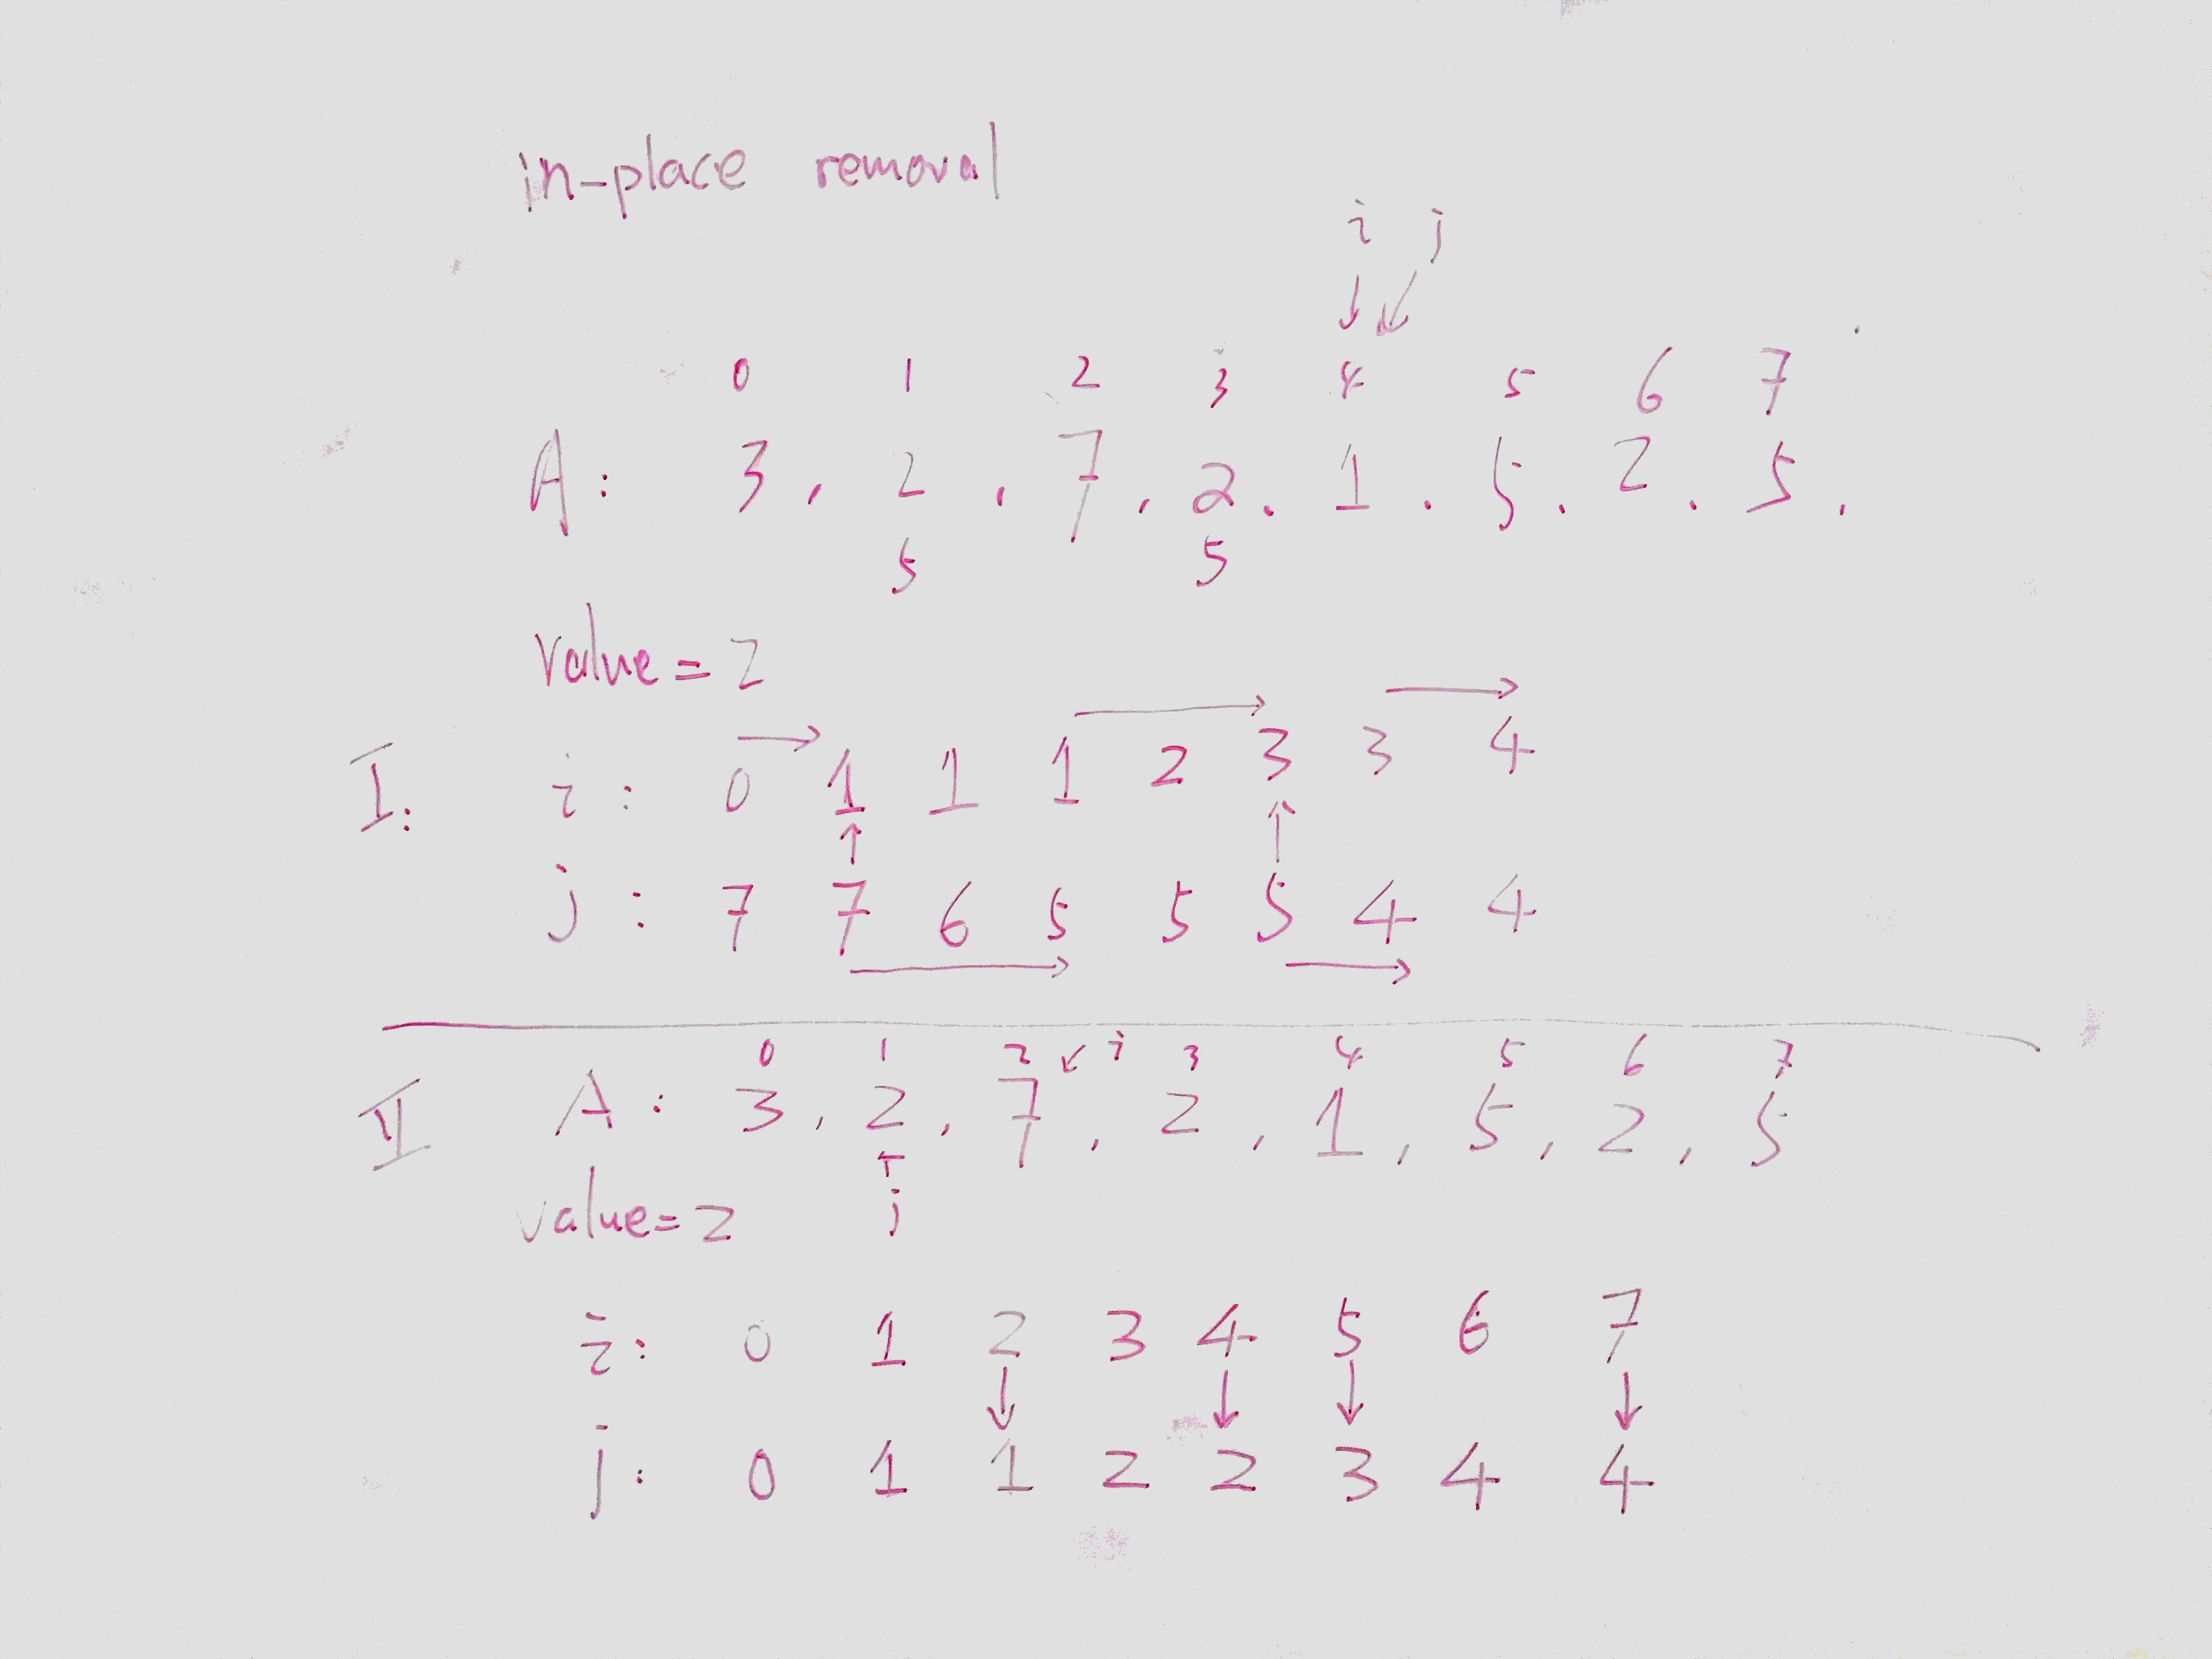
\includegraphics[width=\textwidth]{leetcode27.jpg}
    \centering \\
\end{figure}

\begin{lstlisting}[language=Python, caption=Problem27. Remove Element]

class Solution(object):
    def removeElement_start_end(self, nums, val): # O(n) time
        if len(nums)==0: return 0
        i, j = 0, len(nums)-1
        while i<j:
            if nums[i] != val: i+=1
            else:
                while i<j and nums[j]==val:
                    j-=1
                if i==j: return i
                else: 
                    nums[i] = nums[j]
                    j-=1
                while i<j and nums[j]==val:
                    j-=1
        if nums[i]==val: return i
        else: return i+1
        
    def removeElement_start_start(self, nums, val): # O(n) time
        """
        :type nums: List[int]
        :type val: int
        :rtype: int
        """
        if len(nums) == 0: return 0
        i = j = 0
        while i<len(nums):
            if nums[i] != val:
                nums[j] = nums[i]
                j+=1
            i+=1
        return j
\end{lstlisting}





\subsubsection{leetcode 31. Next Permutation}
Implement next permutation, which rearranges numbers into the \textbf{lexicographically next greater} permutation of numbers. If such arrangement is \textbf{not possible}, it must rearrange it as the \textbf{lowest possible order} (ie, sorted in ascending order). The replacement must be \textbf{in-place}, do \textbf{not allocate extra memory}.\\

\noindent Here are some examples. Inputs are in the left-hand column and its corresponding outputs are in the right-hand column.
\begin{itemize}
    \item $1,2,3 \to 1,3,2$
    \item $3,2,1 \to 1,2,3$
    \item $1,1,5 \to 1,5,1$
\end{itemize}


\begin{CJK*}{UTF8}{gbsn}
\noindent 解题思路:这道题给出的例子有一定的误导性,所以分析之后容易设计出有缺陷的算法。可以找到更有代表性的例子进行分析:$[3,2,6,5,1] \to [3,5,1,2,6]$。分析过程如下图所示:目标是要找到$[3,2,6,5,1]$在递增排列中的下一个排列。我们知道当目标序列从左到右各数字是按照递减序列给出的,那么这个目标序列就已经是由这些数字能够构成的所有排列中最大的一个,这也暗示我们\textbf{可以通过检测这种自左向右递减(或者,自右向左递增)的性质}来设计算法。

\noindent 因为需要找到目标序列的下一个而且更大的排列,所以检测自右向左递增性质比较可行。具体步骤如下:
\begin{itemize}
    \item 首先,自右向左检测目标序列,如果发现某个位置$i$处的数字导致递增的性质结束,那么它就是我们需要替换的数字,具体说就是用一个更大的数字替换它。那么哪一个数字替换它呢?这数字应该从它在目标序列中所在位置的右侧,也就是我们遍历过的数字中寻找。而寻找的策略依旧是自右向左再次遍历这个序列,如果在位置$j$处找到第一个比$i$处大的数值,那么就交换$i$和$j$两个位置的值。比如,上面例子中,5是右侧子序列中第一个比2大的数值,那么两者交换位置,得到新序列$[3,5,6,2,1]$;
    \item 接下来,因为32651是所有32xxx形数值中最大的一个,所以在交换2和5之后,35xxx序列中最小的一个才是32651的下个一序列。进一步观察可以发现,子序列由651变为621,但是序列原有的递增性质没有改变,因此序列621仍然是由6,2,1三个数构成的所有序列中最大的一个,而我们需要则是最小的那个,因此直接反转这个子序列就可以得到所需的最小序列,即126。这样,我们最后得到的结果就是35126,即使题目要求的结果。
\end{itemize}
\noindent 根据上面的分析,需要遍历数组两次:第一次寻找从后向前递增性质消失的位置;第二次再次从后向前寻找替换元素。如果考虑反转子序列的时间代价,整个算法的时间复杂度就是$O(3n)$,即$O(n)$。
\end{CJK*}

\begin{figure}[h]
    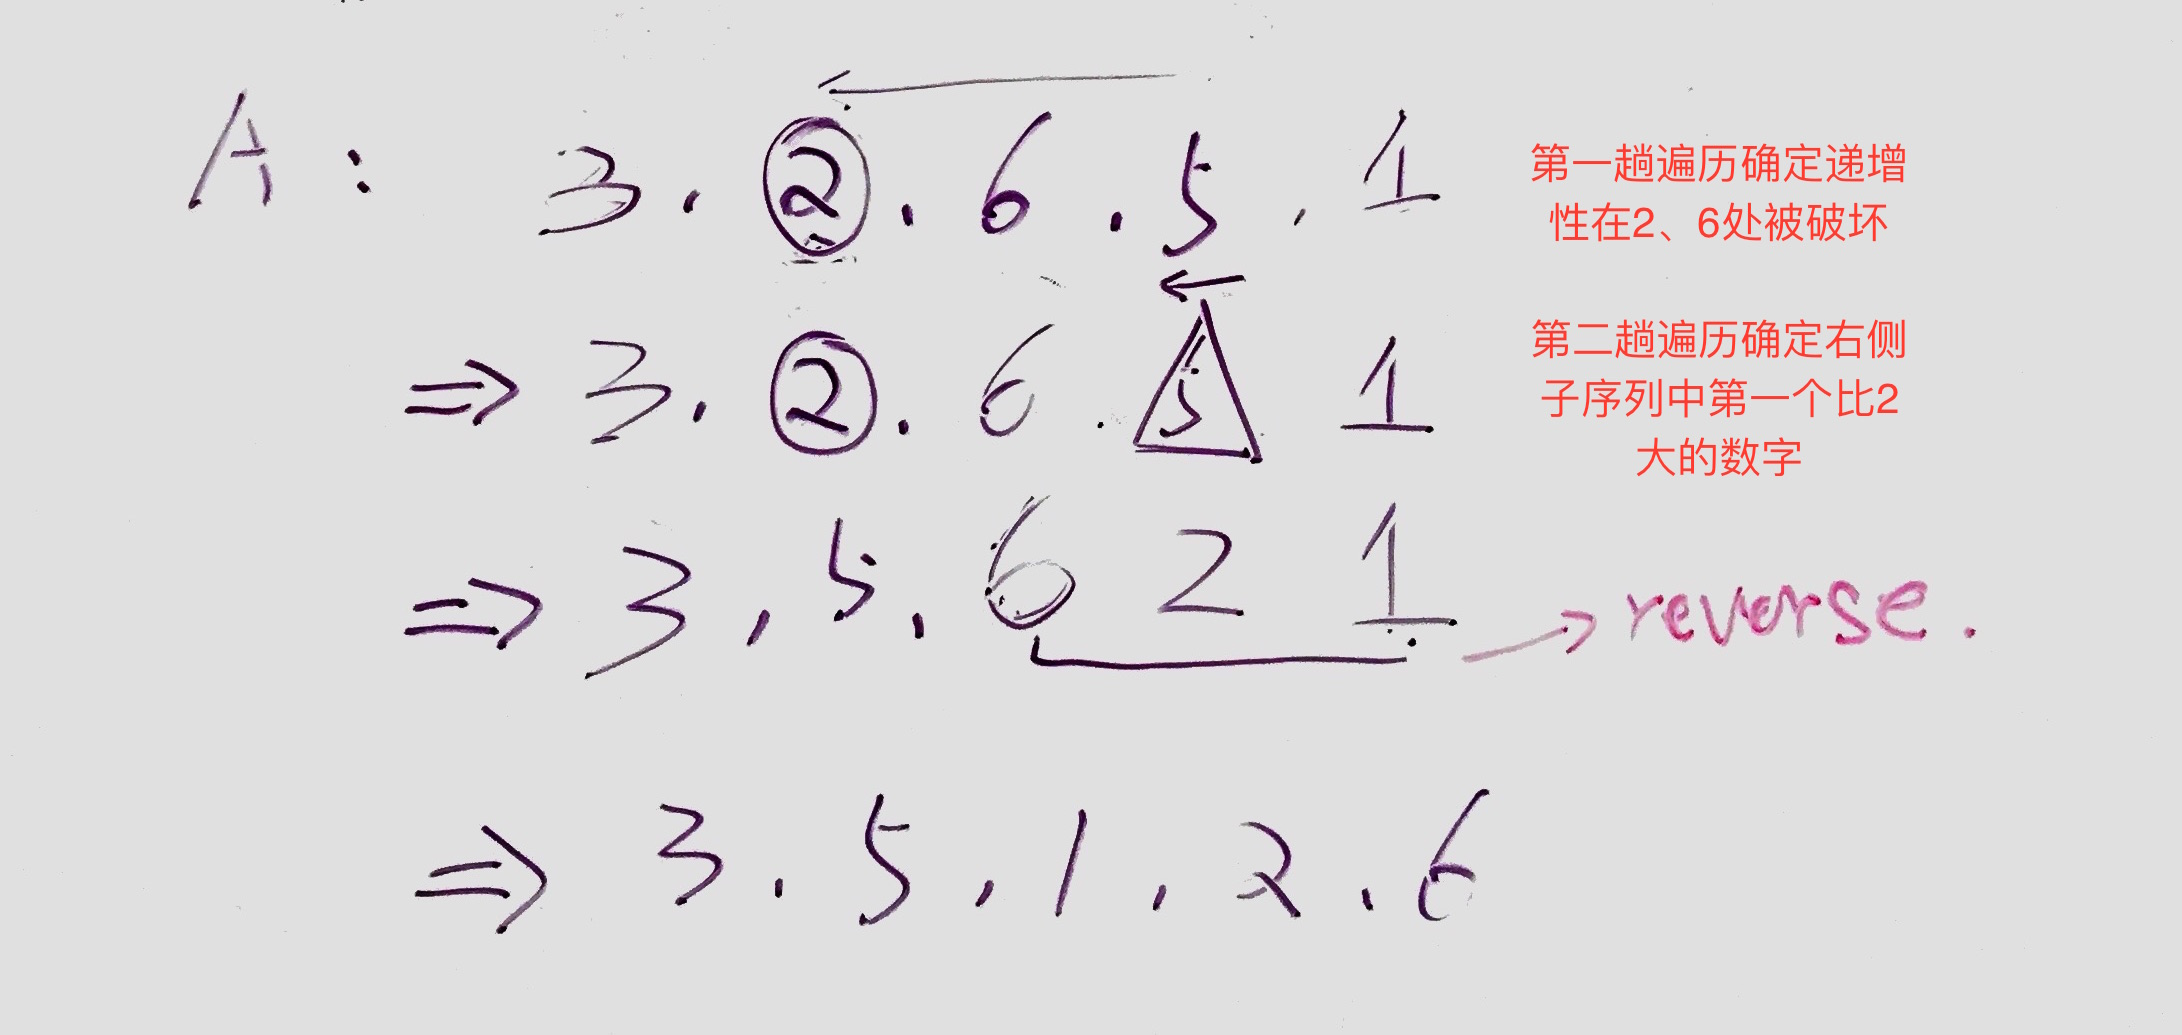
\includegraphics[width=\textwidth]{leetcode31.jpg}
    \centering \\
\end{figure}

\begin{lstlisting}[language=Python, caption=Problem31. Next Permutation]

class Solution(object):
    def nextPermutation(self, nums):    # O(n)
        """
        :type nums: List[int]
        :rtype: void Do not return anything, modify nums in-place instead.
        """
        i = len(nums)-1
        # From right to left, find the first digit 
        # (PartitionNumber) which violate the increase 
        # trend
        while i > 0:
            if nums[i] > nums[i-1]: break
            i -= 1
        if i == 0:
            nums.reverse()
        else:
            # From right to left, find the first digit (ChangeNumber), 
            # which is larger than PartitionNumber; then, swap 
            # ChangeNumber and PartitionNumber
            for k in xrange(len(nums)-1, i-1, -1):
                if nums[i-1] < nums[k]:
                    nums[i-1], nums[k] = nums[k], nums[i-1]
                    break

            # Reverse all digits on the right side of partition index
            nums[i:] = nums[i:][::-1]
\end{lstlisting}


\subsubsection{leetcode 60. Permutation Sequence}

The set [1,2,3,…,n] contains a total of $n!$ unique permutations. By listing and labeling all of the permutations \textbf{in order}, We get the following sequence (ie, for n = 3): "123", "132", "213", "231", "312", "321". Given $n$ and $k$, return the $k^{th}$ permutation sequence.\\

\begin{CJK*}{UTF8}{gbsn}
\noindent 解题思路:假设n = 6,k = 400:
\begin{itemize}
    \item 先计算第一位: 第一位为6,那么它最少也是第 $5! \times 5+1$ 个排列,这是因为第一位为1/2/3/4/5时,都有5!个排列,因此第一位为6时,至少是第$5! \times 5 + 1$个排列(这个排列为612345)。$5! \times 5 + 1 = 601 > k$,所以第一位不可能是6。一个一个地枚举,直到第一位为4时才行,这时,4xxxxx 至少为第 $5! \times 3 + 1 = 361$个排列。
    
    \item 然后计算第二位,与计算第一位时的区别在于,46xxxx至少为第 $4! \times 4 + 1 = 97$个排列,这是因为比6小的只有5/3/2/1了。最后可以计算出第二位为2。
    
    \item 以此类推,最终得出第400个排列为425361。
\end{itemize}
\end{CJK*}

\begin{lstlisting}[language=Python, caption=Problem60. Permutation Sequence]

class Solution(object):
    def getPermutation(self, n, k): # O(n)
        """
        :type n: int
        :type k: int
        :rtype: str
        """
        res = ''
        # compute the factorial of (n-1)
        factorial = 1
        for i in xrange(1,n): 
            factorial *= i
        nums = [x+1 for x in xrange(n)]
        for x in xrange(n-1, 0, -1):
            i = k/factorial
            k = k%factorial
            if k > 0:
                res += str(nums[i])
                nums.remove(nums[i])
            else:
                res += str(nums[i-1])
                nums.remove(nums[i-1])
            factorial = factorial/x
        res += str(nums[0])
        return res
\end{lstlisting}


\subsubsection{leetcode 42. Trapping Rain Water}
Given $n$ non-negative integers representing an elevation map where the width of each bar is 1, compute how much water it is able to trap after raining. For example, 
given [0,1,0,2,1,0,1,3,2,1,2,1], return 6.\\

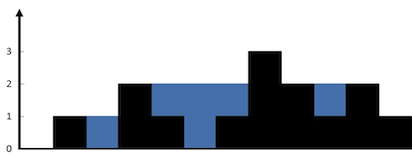
\includegraphics[]{rainwatertrap.png}\\

\begin{CJK*}{UTF8}{gbsn}
\noindent 解题思路:开辟两个数组leftmost和rightmost,leftmost[i]表示在height[i]处之前(包括$i$)出现过的最高的bar值,而rightmost[i]表示在height[i]处之后(包括$j$)出现过的最高的bar值。假设在某个$i$位置处,当leftmost[i]和rightmost[i]都大于height[i]时,那么leftmost[i], height[i],和rightmost[i]三者构成一个可以储水的“凹”;而这个“凹”的储水量是以height[i]为“底”,leftmost[i]和rightmost[i]两者中的较小值为有效高度计算得到的,即water = min(leftmost[i], rightmost[i])-height[i]。下面代码的第一个方法实现了上面的设计思路。代码中的第二个方法是对第一个方法的改进,使用了一个同名的变量代替了方法一中的rightmost数组,降低空间复杂度的同时,可以进一步改进效率。下面的示例图给出了方法一的计算过程和及部分图例。
\end{CJK*}

\begin{figure}[h]
    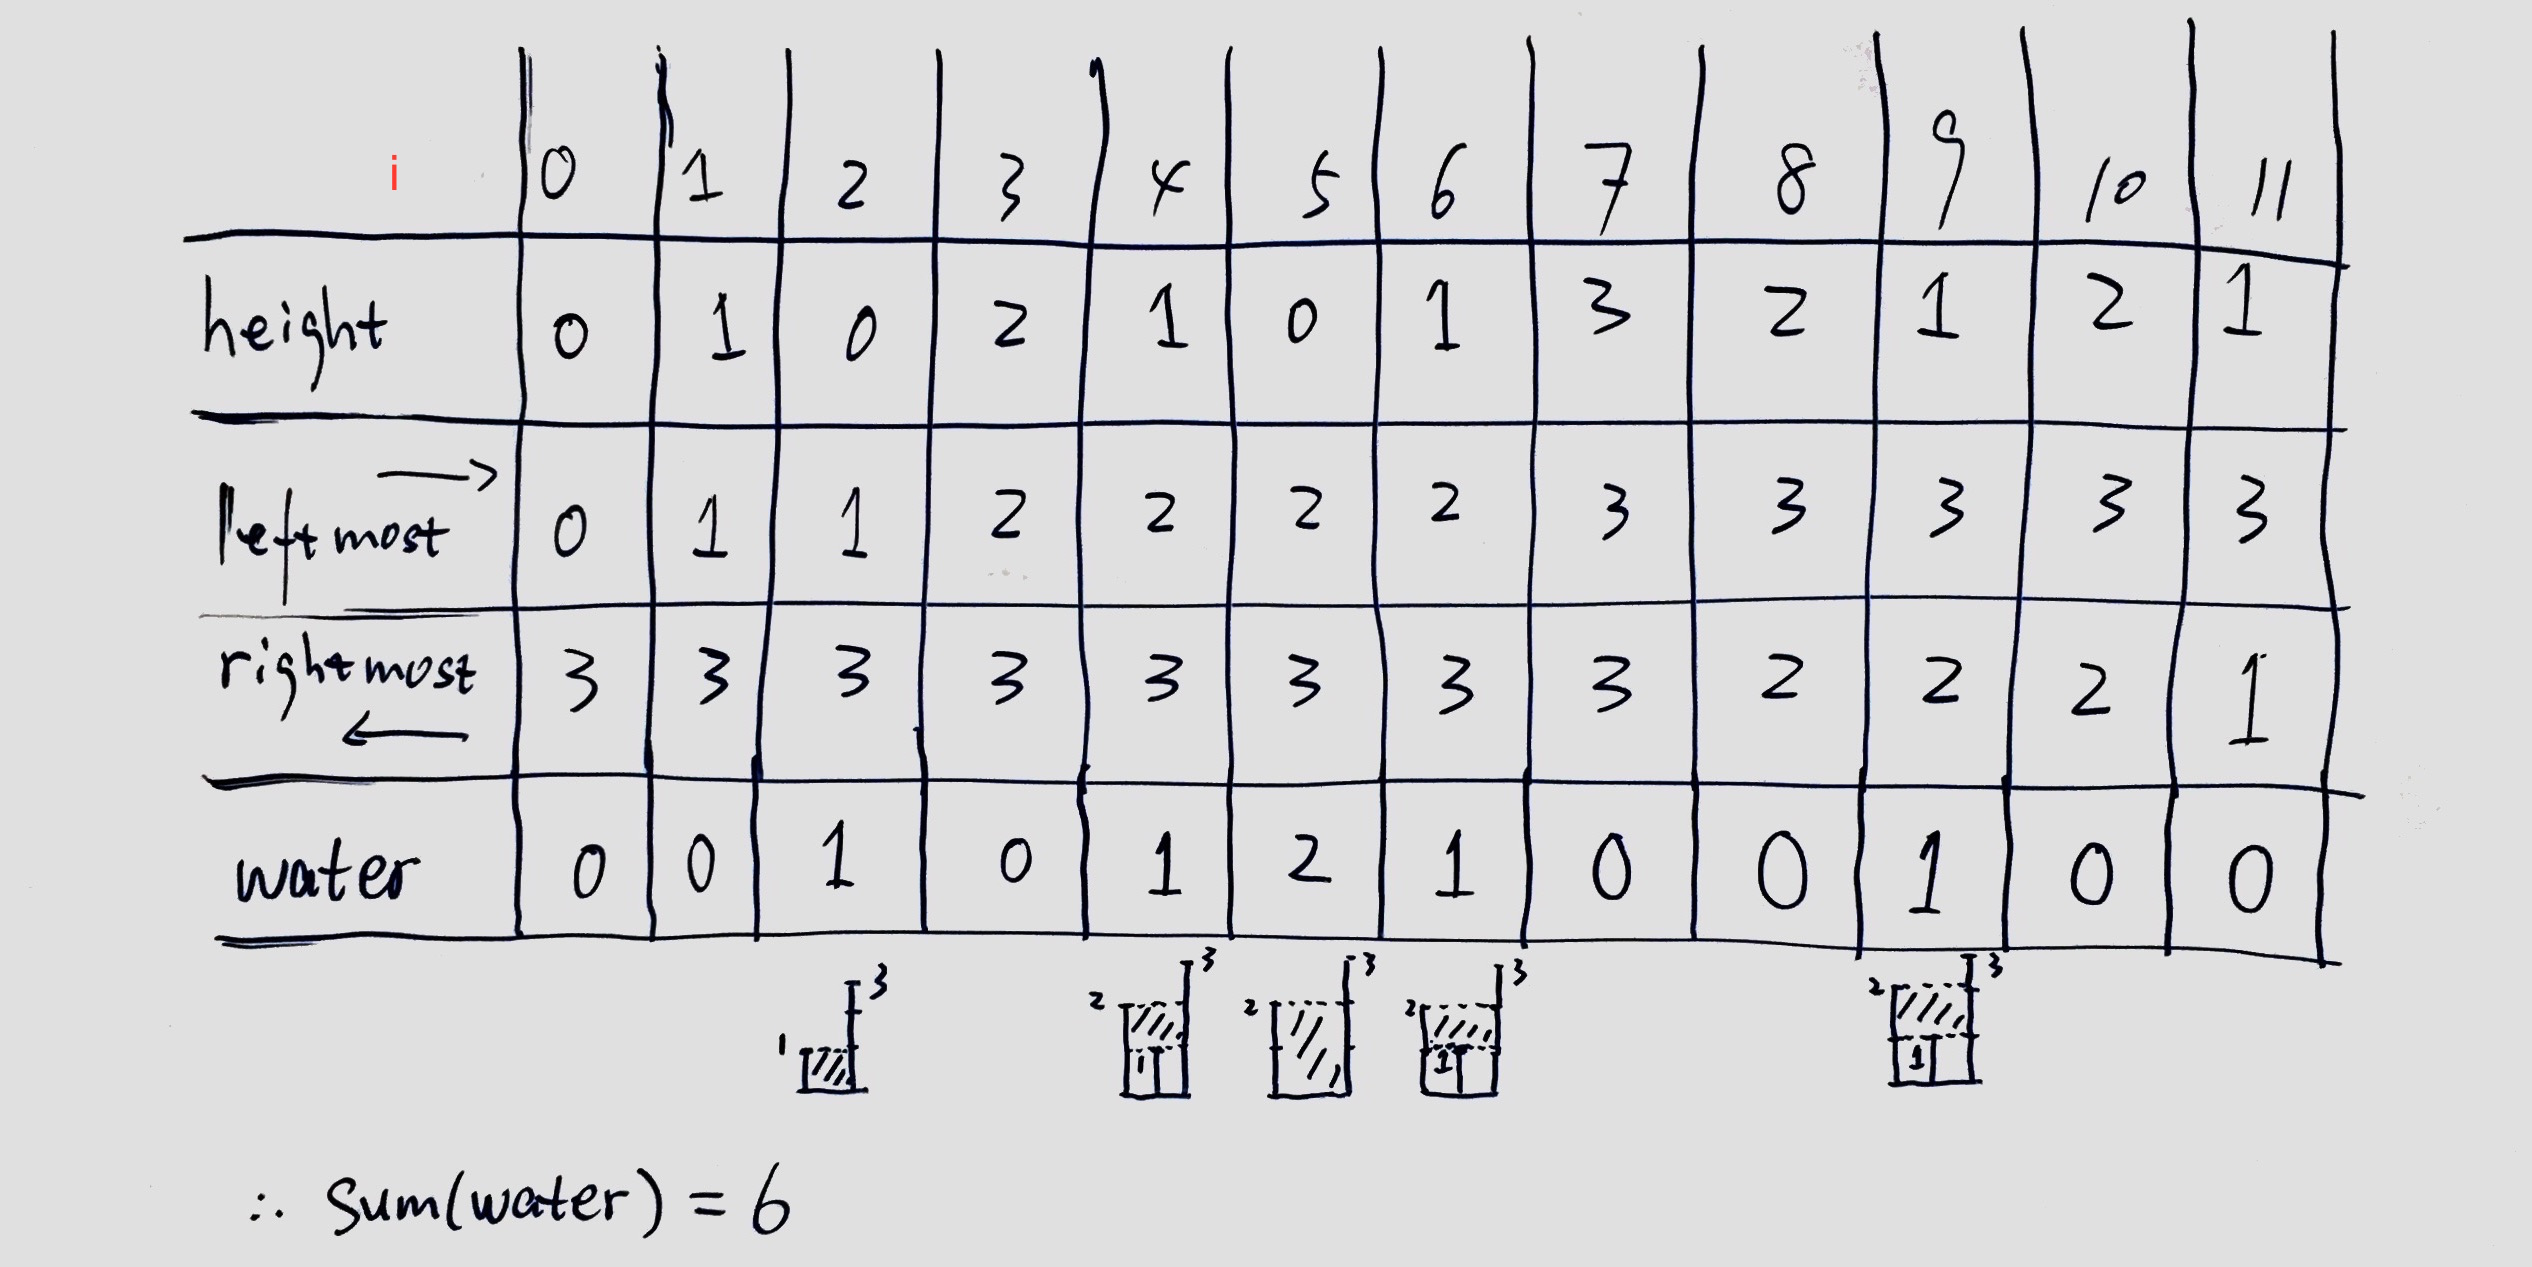
\includegraphics[width=\textwidth]{leetcode42.jpg}
    \centering \\
\end{figure}

\begin{lstlisting}[language=Python, caption=Problem42. Trapping Rain Water]

class Solution(object):
    def trap(self, height):  # O(n) time, O(n) space
        """
        :type height: List[int]
        :rtype: int
        """
        n = len(height)
        if n==0: return 0
        # from left to right, compute leftmost[i],
        # which means the most height on the left
        # side of the i-th position
        leftmost = [height[0]]
        for x in xrange(1, n):
            leftmost.append(max(leftmost[-1], height[x]))
        water = 0
        # rightmost indicates the most height on the
        # right side of the i-th position from right
        # to left
        rightmost = height[n-1]
        for x in xrange(n-1, -1, -1):
            if height[x]<rightmost and height[x]<leftmost[x]:
                water += min(rightmost, leftmost[x]) - height[x]
            elif height[x] > rightmost:
                rightmost = height[x]
        return water
\end{lstlisting}



\subsubsection{leetcode 48. Rotate Image}
You are given an $n \times n$ 2D matrix representing an image. Rotate the image by 90 degrees (clockwise).Follow up: could you do this \textbf{in-place}?\\

\begin{CJK*}{UTF8}{gbsn}
\noindent 解题思路:该任务可以通过两个步骤完成。第一步将原矩阵按照行排列分成上下两个部分,依次交换第一行和最后一行,第二行和倒数第二行,以此类推。第二步按照主对角线依次交换两个对称位置上的元素。第二步结束后即可得到最终结果。

\noindent 进一步扩展这个题目就是求解逆时针旋转90度,那么首先同样完成上面描述的第一步,而第二步是按照次对角线交换对称位置上的一对儿元素。\\
\end{CJK*}

\begin{lstlisting}[language=Python, caption=Problem48. Rotate Image]

class Solution(object):
    def rotate(self, matrix):   # O(n^2)
        """
        :type matrix: List[List[int]]
        :rtype: void Do not return anything, modify matrix in-place instead.
        """
        rows = len(matrix)
        cols = len(matrix[0])
        
        if rows<2 or cols<2:
            return
        
        # invert the matrix
        for j in range(cols):
            for i in range(rows/2):
                matrix[i][j], matrix[rows-1-i][j] = matrix[rows-1-i][j], matrix[i][j]
        
        # flap the matrix along the main diagonal
        # k indicates the starting column when the
        # row changes each time
        k = 0
        for i in range(rows):
            for j in range(k,cols):
                if i!=j:
                    matrix[i][j], matrix[j][i] = matrix[j][i], matrix[i][j]
            k+=1
\end{lstlisting}

\subsubsection{leetcode 66. Plus One}
Given a non-negative number represented as an array of digits, plus one to the number. The digits are \textbf{stored} such that \textbf{the most significant digit} is at the head of the list.\\

\begin{CJK*}{UTF8}{gbsn}
\noindent 解题思路:这道题比较简单,唯一需要留意的是在计算完数组中的每一位后,不要忘记判断进位变量是否为0。在不为0的情况下,需要在最终的结果数组头部增加一个位置,存放进位变量的值。\\
\end{CJK*}

\begin{lstlisting}[language=Python, caption=Problem66. Plus One]

class Solution(object):
    def plusOne(self, digits):  # O(n)
        """
        :type digits: List[int]
        :rtype: List[int]
        """
        n = len(digits)
        carry = 1
        for x in xrange(n-1,-1,-1):
            val = digits[x] + carry
            carry = val / 10
            digits[x] = val % 10
        if carry == 1:
            digits = [1] + digits
        return digits
\end{lstlisting}


\subsubsection{leetcode 70. Climbing Stairs}

You are climbing a stair case. It takes n steps to reach to the top. Each time you can either climb 1 or 2 steps. In how many distinct ways can you climb to the top?\\

\begin{CJK*}{UTF8}{gbsn}
\noindent 解题思路:这道题就是比较典型的决策问题,使用DFS遍历决策树。与Fibonacci Number的求解思路一致。这道题的另一种解题方法就是用DP算法,改进DFS算法的重复计算问题。下面代码给出两种DP算法的实现,两者的区别在于不同的空间复杂度。但是,两种算法的状态转换方程相同:dp[n]=dp[n-1]+dp[n-2], dp[i]表示i个台阶的时候有多少种不同的走法。\\
\end{CJK*}

\begin{lstlisting}[language=Python, caption=Problem70. Climbing Stairs]

class Solution(object):
    def climbStairs_dp1(self, n): # RT:O(n), Space: O(n)
        dp = [0 for _ in xrange(n+1)]
        dp[0] = 1
        dp[1] = 1
        for x in xrange(2, n+1):
            dp[x] = dp[x-1]+dp[x-2]
        return dp[n]
        
    def climbStairs_dp2(self, n): # RT: O(n), Space: O(1)
        """
        :type n: int
        :rtype: int
        """
        if n==1: return 1
        if n==2: return 2

        a,b,c = 1,2,0
        for i in range(2, n):
            c = a + b
            a,b = b,c
        return c
\end{lstlisting}



\subsubsection{leetcode 89. Gray Code}
The gray code is a binary numeral system where two successive values differ in only one bit. Given a non-negative integer $n$ representing the total number of bits in the code, print the sequence of gray code. A gray code sequence must begin with 0. \\

\noindent For example, given n = 2, return [0,1,3,2]. Its gray code sequence is:
\begin{itemize}
    \item 00 - 0, 01 - 1, 11 - 3, 10 - 2
\end{itemize}

\begin{CJK*}{UTF8}{gbsn}
\noindent 解题思路:Gray Code是啥都不知道,这道题只能求助万能的wikipedia了。Wikipedia上给出的reflect-and-prefix方法很有趣,这里提供了来自wikipedia的示例图来说明这个方法的思想。从下面的示例图也可以看出,由$n$产生的gray code序列数量是$2^n$个。
\end{CJK*}

\begin{figure}[h]
    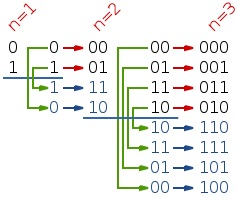
\includegraphics[width=6cm]{leetcode89.jpg}
    \centering \\
\end{figure}

\begin{lstlisting}[language=Python, caption=Problem89. Gray Code]

class Solution(object):
    def grayCode(self, n): # RT: O(n)
        res=[]
        size=1<<n
        for i in range(size):
            res.append((i>>1)^i)
        return res
\end{lstlisting}


\subsubsection{leetcode 73. Set Matrix Zeroes}
Given a $m \times n$ matrix, if an element is 0, set its entire row and column to 0. Do it \textbf{in place}. \\

\noindent Follow up: Did you use extra space? A straight forward solution using $O(mn)$ space is probably a bad idea. A simple improvement uses $O(m + n)$ space, but still not the best solution. Could you devise a constant space solution?\\

\begin{CJK*}{UTF8}{gbsn}
\noindent 解题思路:这道题实际就是考查设计DP算法。这里给出一个示例图,图中使用了比题目要求更少的额外空间,即$O(m+n)$,但是计算复杂度会有所增加。这里展示的这种额外空间的设计思路是和Leetcode51 N-Queens系列题目的做个类比,实际就是相同的想法:用一维数组表示每行的信息,而第$i$个cell中的数值$j$表示目标矩阵中第$i$行、第$j$列的某种或某类对解题有益的属性。\\

\noindent这道题的另外一种$O(1)$空间复杂度的设计方法就是利用现有矩阵进行存储,即利用第一行和第一列的某些位置。根据问题描述,在某行(列)存在0时,整行(列)都要置为0,所以这一行(列)的第一个位置就可以作为临时的标志位。
\end{CJK*}

\begin{figure}[h]
    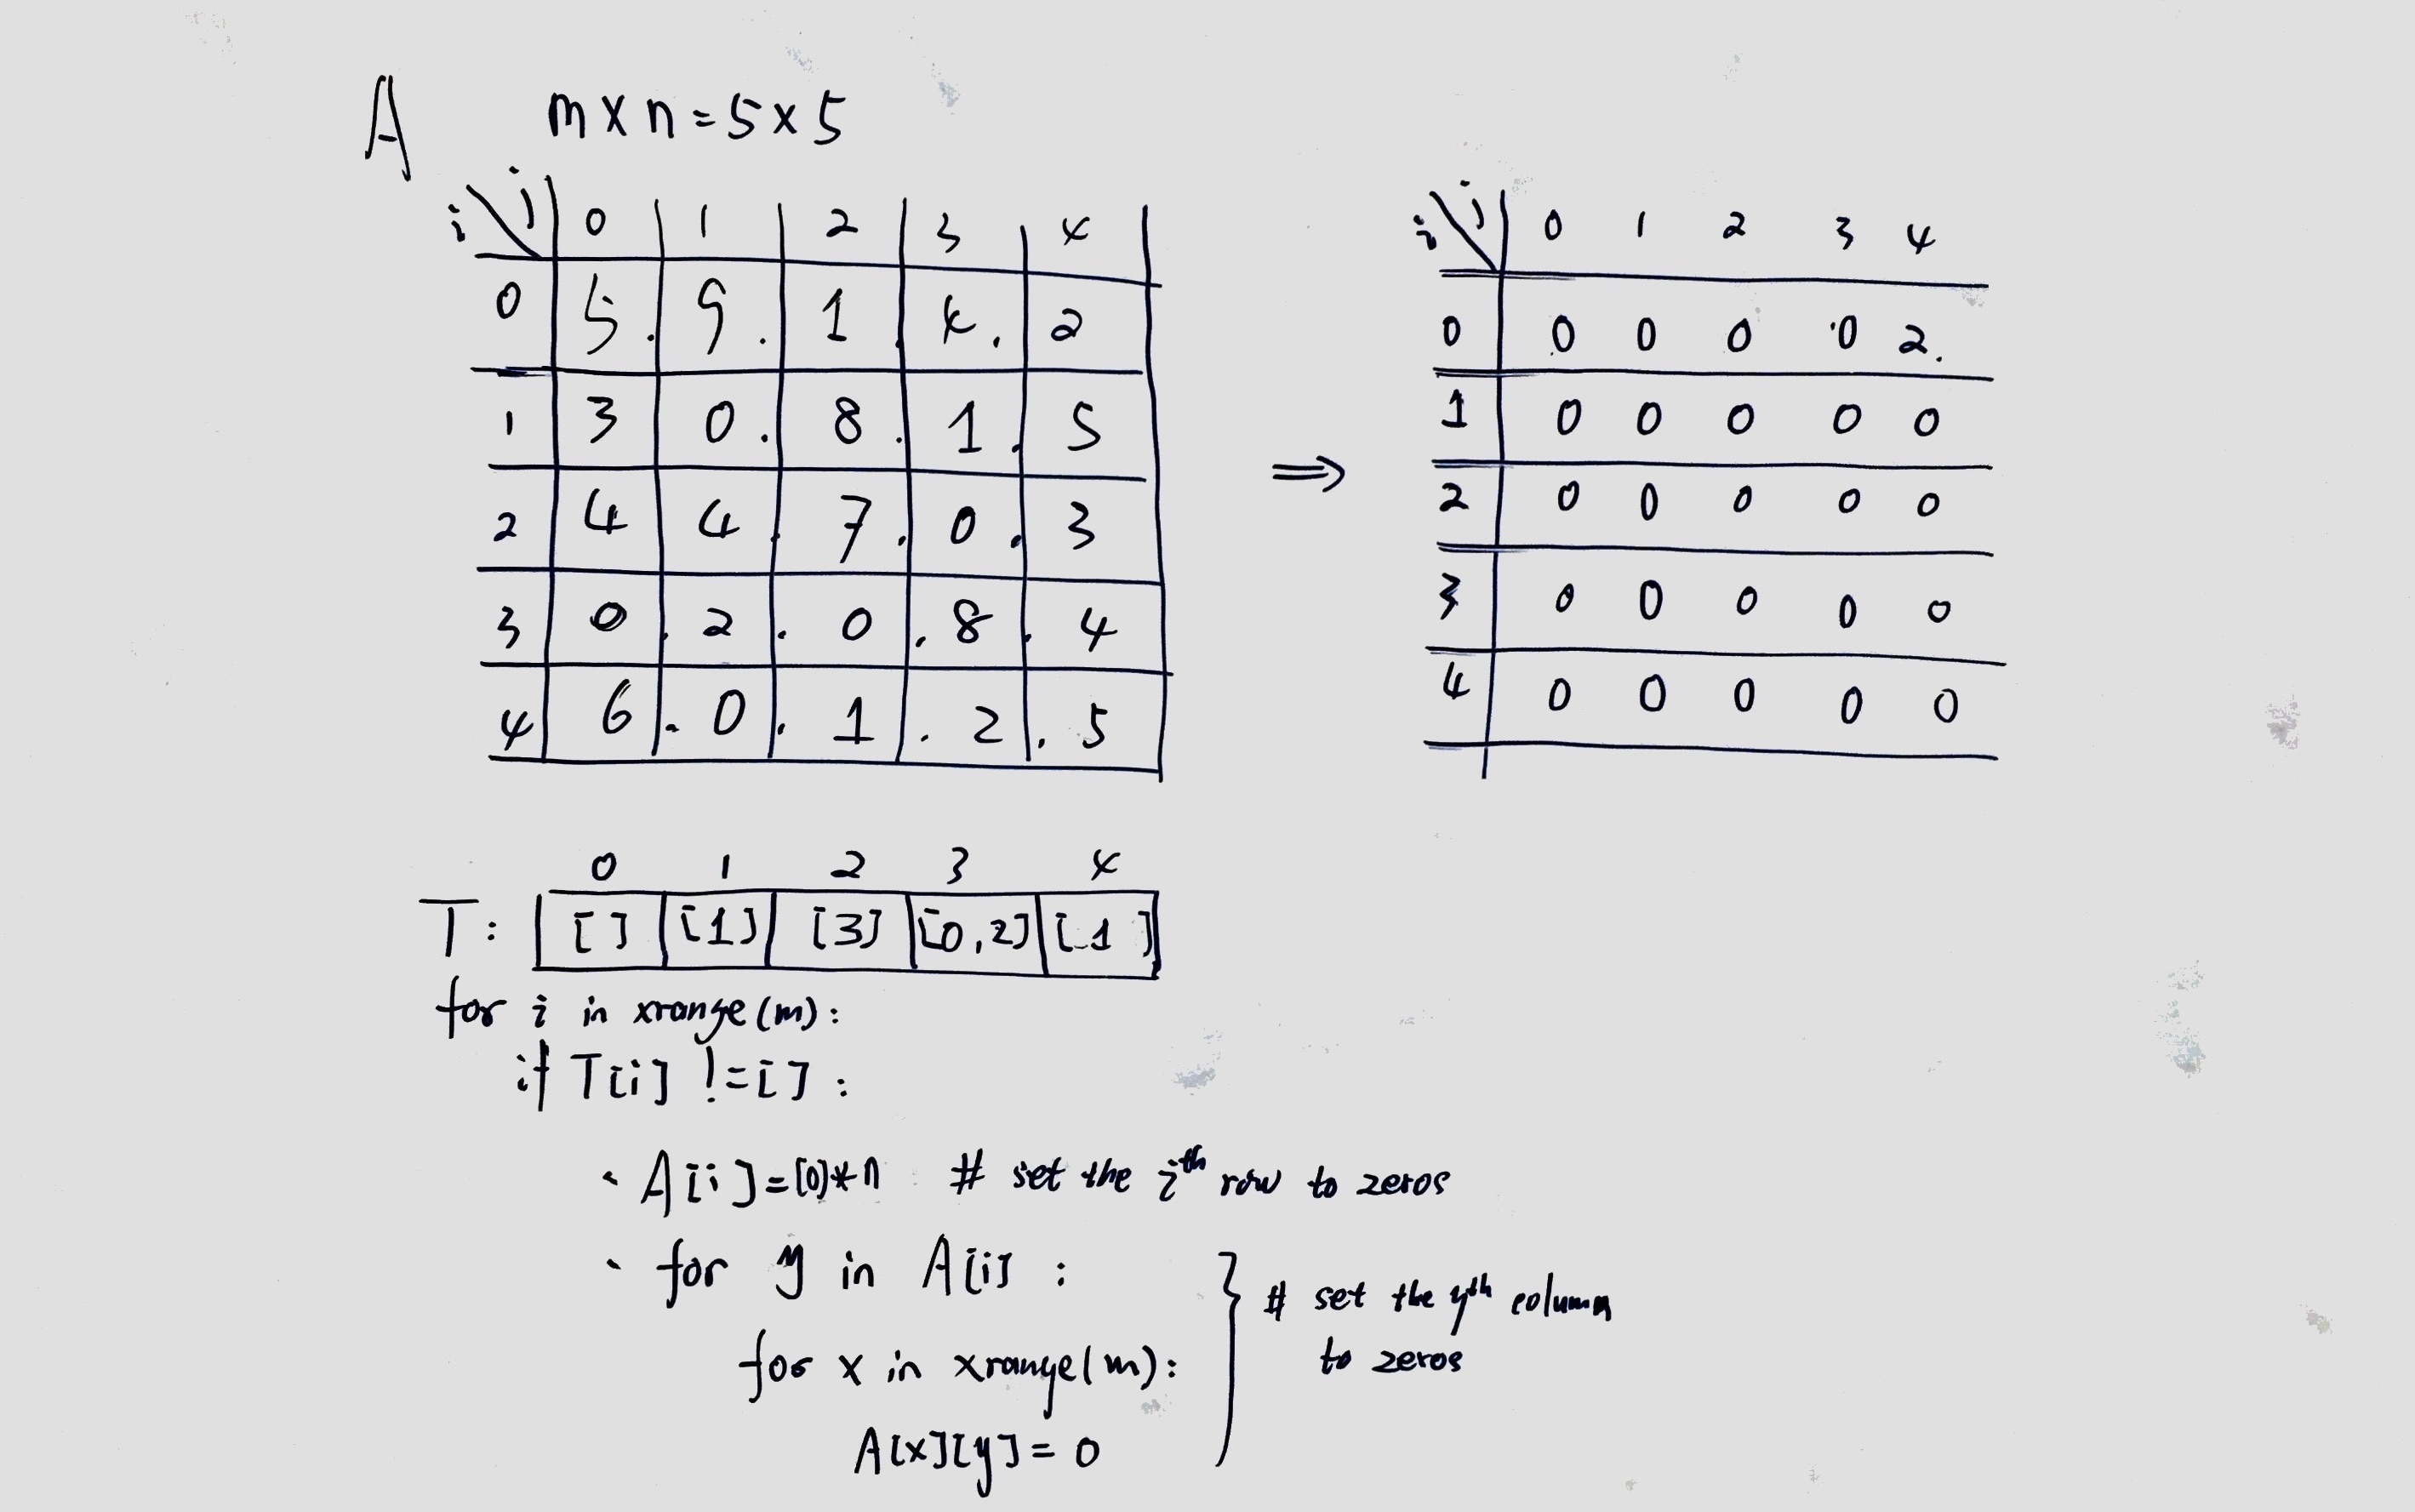
\includegraphics[width=\textwidth]{leetcode73.jpg}
    \centering \\
\end{figure}

\begin{lstlisting}[language=Python, caption=Problem73. Set Matrix Zeroes]

class Solution(object):
    def setZeroes(self, matrix):    # Time:O(m*n), Space:O(m+n)
        """
        :type matrix: List[List[int]]
        :rtype: void Do not return anything, modify matrix in-place instead.
        """
        m,n = len(matrix), len(matrix[0])
        zerorows = [False for _ in xrange(m)]
        zerocols = [False for _ in xrange(n)]

        for x in xrange(m):
            for y in xrange(n):
                if matrix[x][y] == 0:
                    zerorows[x], zerocols[y] = True, True

        for x in xrange(m):
            for y in xrange(n):
                if zerorows[x] or zerocols[y]:
                    matrix[x][y] = 0
\end{lstlisting}


\subsubsection{leetcode 134. Gas Station}
There are N gas stations along a circular route, where the amount of gas at station $i$ is gas[$i$]. You have a car with an \textbf{unlimited} gas tank and it costs cost[$i$] of gas to travel from station $i$ to its next station $i+1$. You begin the journey with an empty tank at one of the gas stations. Return the starting gas station's index if you can travel around the circuit once, otherwise return -1. Note: The solution is guaranteed to be \textbf{unique}.\\

\begin{CJK*}{UTF8}{gbsn}
\noindent 解题思路:要想完成一圈必须满足两个条件:
\begin{enumerate}
    \item 首先,需要验证加油站总油量是否能够满足总消耗量;
    \item 其次,在每一个加油站,判断当前剩余油量与当前加油站能够提供的油量的总和是否可以完成接下来的消耗;如果不满足,那么说明当前的起点无法完成整个旅程,就要设置起点为下一个加油站。
\end{enumerate}
在分析问题的时候,可能会有这种疑问:会不会在环上有两条边的耗油量cost[i]和cost[j]分别大于其对应的起点加油站的储油量gas[i]和gas[j],造成没法完成环路?这种情况实际是通过第一个条件是否成立来保证。如果油站的总储油量大于总消耗量,那么邮箱里剩下的油量加上最后一次加的油量一定可以完成总路程。此外,题目描述中有一个重要条件,油箱的加油量没有限制,所以就可以保证每次都可以把当前油站的所有油量都加入车内。如果没有这个条件,那么即使总油量大于总耗油量,也不一定能完成环路。\\
\end{CJK*}


\begin{lstlisting}[language=Python, caption=Problem134. Gas Station]

class Solution(object):
    def canCompleteCircuit(self, gas, cost):    # running time is O(n)
        """
        :type gas: List[int]
        :type cost: List[int]
        :rtype: int
        """
        if sum(gas)<sum(cost): return -1
        station = 0
        diff = 0
        for i in range(len(gas)):
            if diff+gas[i]<cost[i]:
                station = i+1
                diff = 0
            else:
                diff = diff+gas[i]-cost[i]
        
        return station
\end{lstlisting}

\begin{figure}[h]
    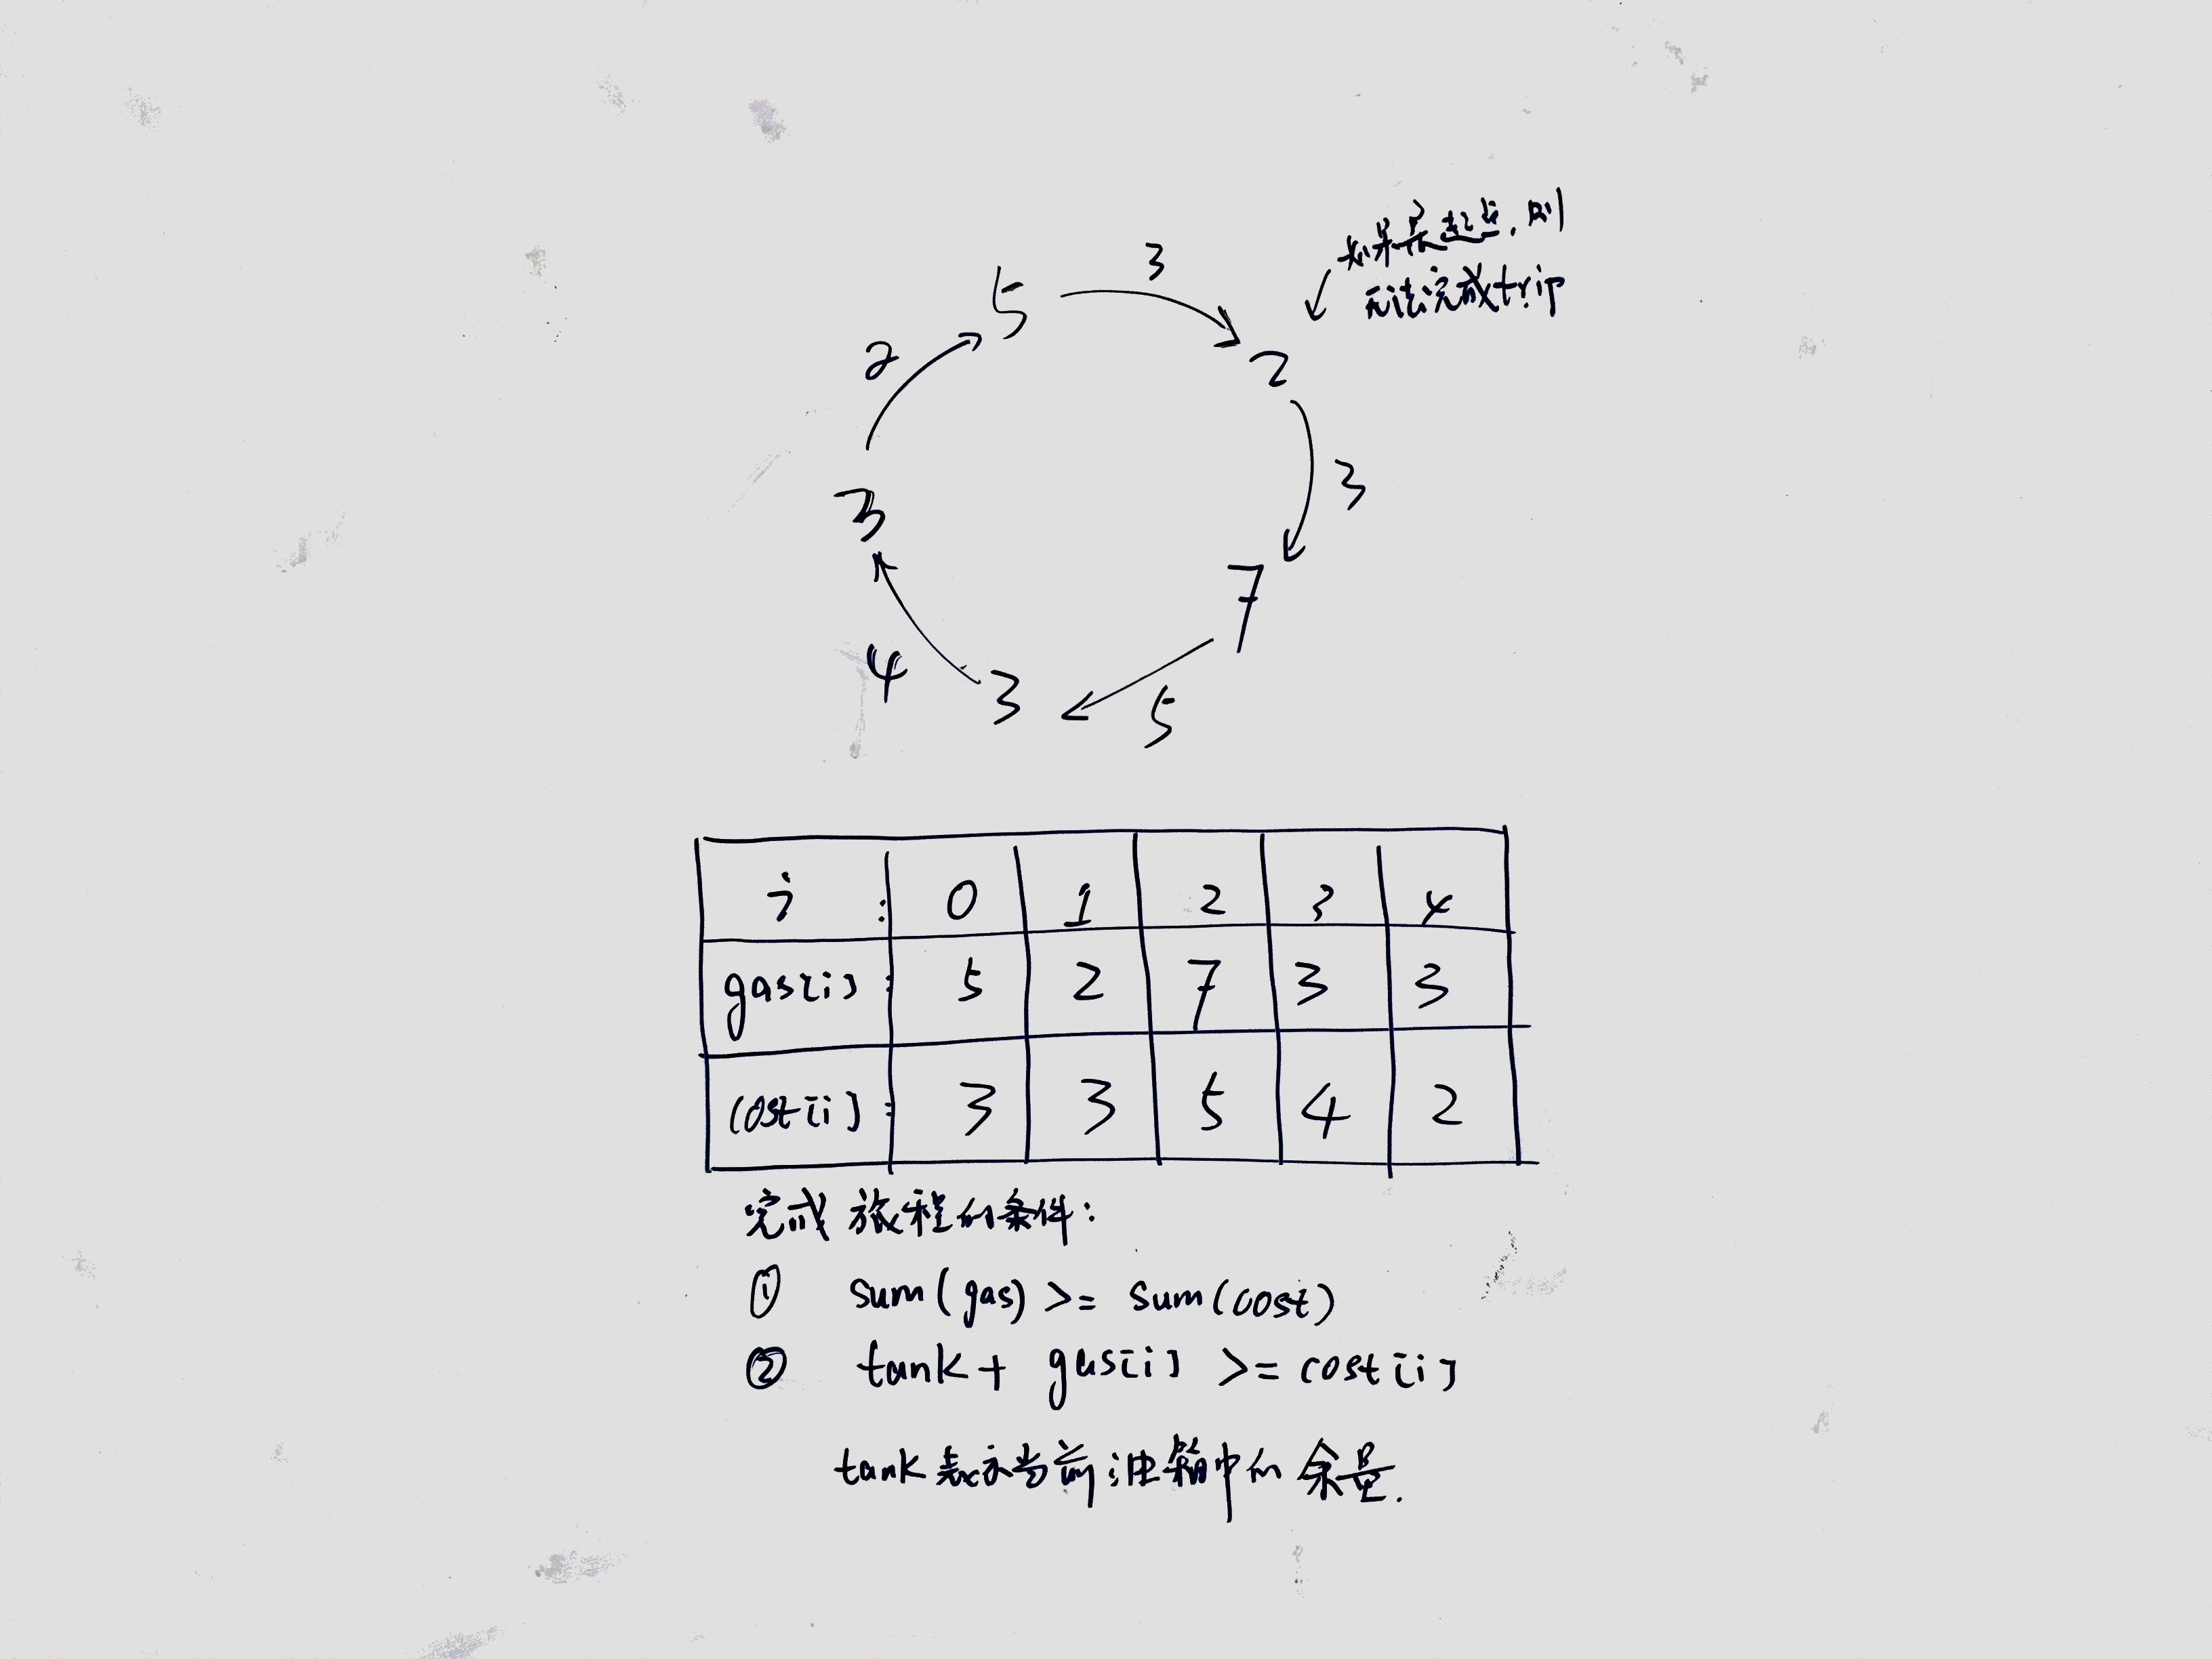
\includegraphics[width=10cm]{leetcode134.jpg}
    \centering \\
\end{figure}


\subsubsection{leetcode 135. Candy}
There are $N$ children standing in a line. Each child is assigned a rating value. You are giving candies to these children subjected to the following requirements:
\begin{itemize}
    \item Each child must have \textbf{at least} one candy.
    \item Children with a \textbf{higher rating get more} candies than their neighbors.
    \item What is the \textbf{minimum} candies you must give?
\end{itemize}

\begin{CJK*}{UTF8}{gbsn}
\noindent 解题思路:求最少的糖数。首先,给每个孩子一枚糖,保证每个孩子都有糖的要求;然后,保证等级比旁边孩子高的孩子获得等多的糖。那么“旁边”就分为左右两边,因此我们首先从左向右遍历数组,保证所有等级比其左边孩子高的孩子(除去左边第一个孩子),可以获得(比其左边孩子)多一枚糖;同理,为了保证所有等级比其右边孩子高的孩子(除去右边第一个孩子),可以获得(比其右边孩子)多一枚糖,再从右向左遍历数组一次;但是需要注意,题目要求最小数量的糖果,所以在从右向左遍历时,在判断等级的同时,还需要同时判断当前孩子手里的糖果数量是否少于其右侧孩子拥有的糖果数量。所以,等级高过右侧孩子,不意味着一定再次发糖。参考下面的示例图。\\
\end{CJK*}

\begin{lstlisting}[language=Python, caption=Problem135. Candy]

class Solution(object):
    def candy(self, ratings):   # RT: O(n)
        """
        :type ratings: List[int]
        :rtype: int
        """
        n = len(ratings)
        candynum = [1 for _ in range(n)]
        
        for i in xrange(1, n):
            if ratings[i] > ratings[i-1]:
                candynum[i] = candynum[i-1] + 1
        
        for i in reversed(range(n-1)):
            if ratings[i] > ratings[i+1] and candynum[i] <= candynum[i+1]:
                candynum[i] = candynum[i+1] + 1
        
        return sum(candynum)
\end{lstlisting}

\begin{figure}[h]
    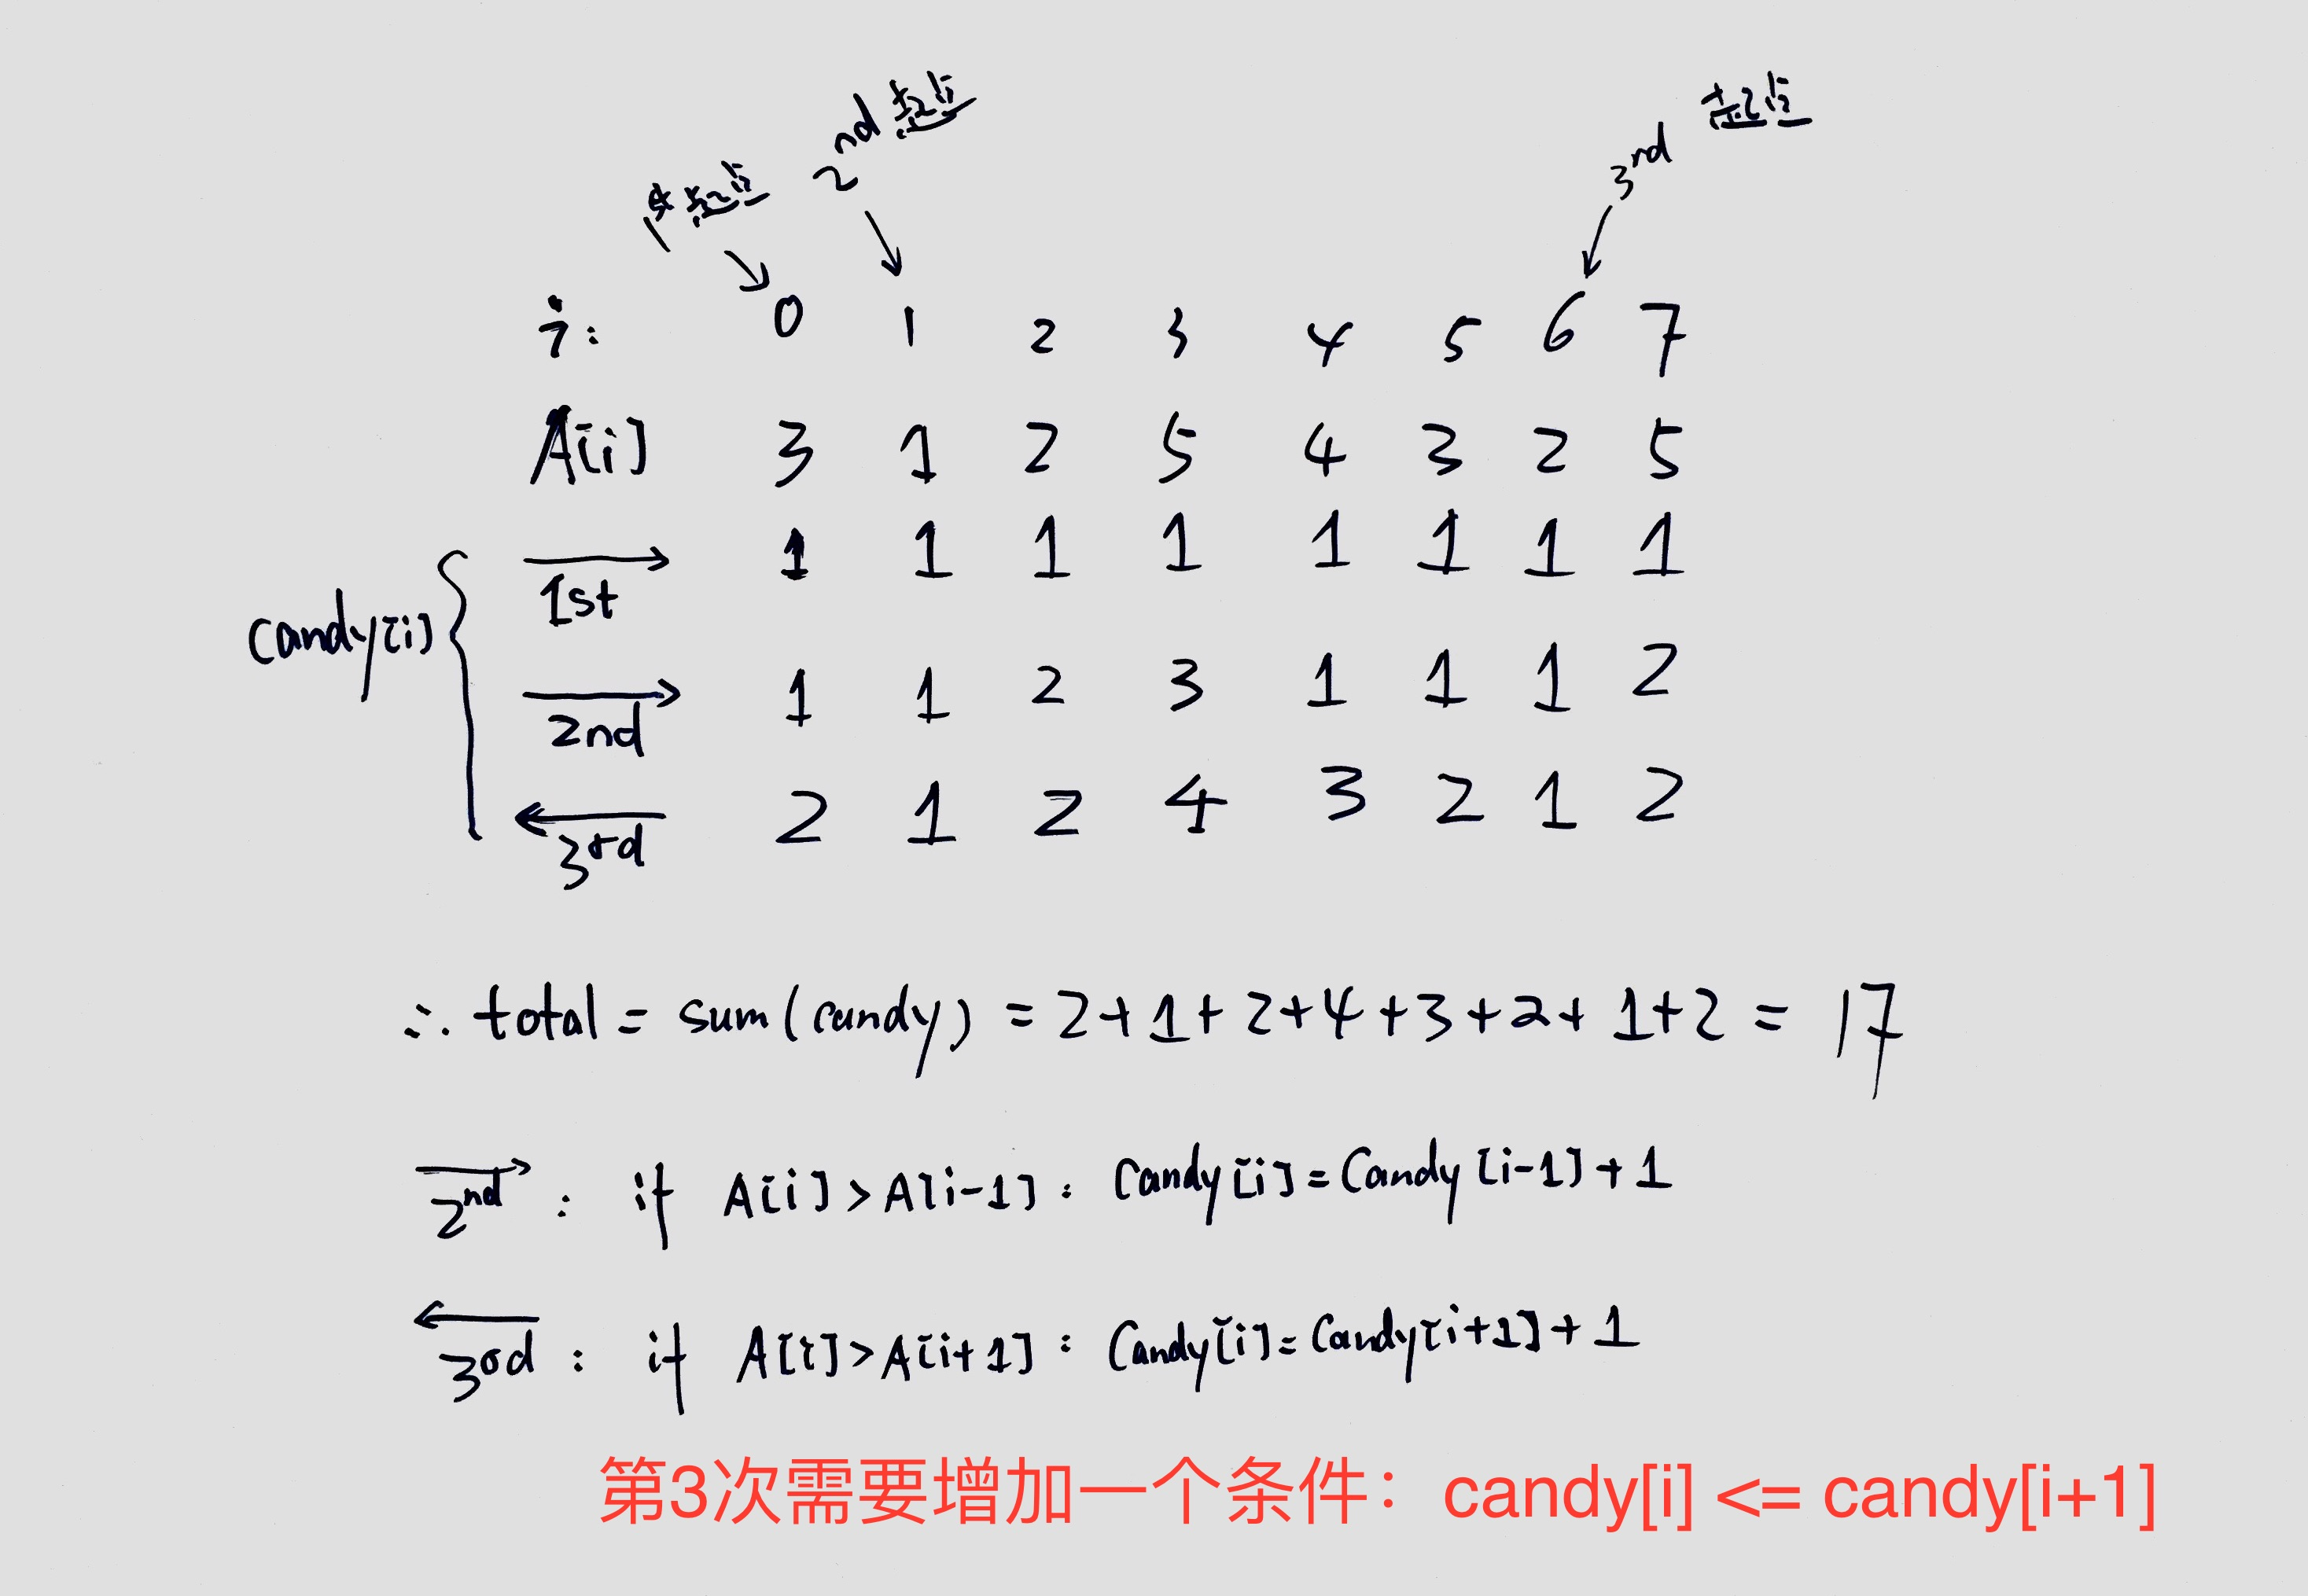
\includegraphics[width=\textwidth]{leetcode135.jpg}
    \centering \\
\end{figure}



\subsubsection{leetcode 136. Single Number}
Given an array of integers, every element appears \textbf{twice} except for one. Find that single one. Note: Your algorithm should have a \textbf{linear} runtime complexity. Could you implement it \textbf{without using extra memory}?\\

\begin{CJK*}{UTF8}{gbsn}
\noindent 解题思路:这道题的额外提示要求不使用额外空间就可以获得结果,所以可以明确这个题目的考点应该不是设计hashtable这类的数据结构来解题。这题考查的是位操作,需要明白基本位运算(与、或、非、异或、同或)的意义。针对这道题的描述,存在偶数个重复元素,而只有一个元素出现一次,所以使用异或(xor)操作就可以解决问题。异或操作的定义为:x XOR 0 = x; x XOR x = 0。如果重复元素是奇数个呢?(leetcode137)
\end{CJK*}\\

\begin{lstlisting}[language=Python, caption=Problem136. Single Number]

class Solution(object):
    def singleNumber(self, nums):
        """
        :type nums: List[int]
        :rtype: int
        """
        # basic XOR operations: x^x=0, x^0=x
        # Suppose nums=[2,2,3,4,4], 2^2^3^4^4=(2^2)^3^(4^4)=3
        # Suppose nums=[2,1,3,2,3], 2^1^3^2^3=3^2^3=1^3=1
        sn = nums[0]
        for i in range(1, len(nums)):
            sn = sn ^ nums[i]
        
        return sn
\end{lstlisting}


\subsubsection{leetcode 137. Single Number II}
Given an array of integers, every element appears \textbf{three} times except for one. Find that single one. Note: Your algorithm should have a \textbf{linear} runtime complexity. Could you implement it \textbf{without using extra memory}?\\

\begin{CJK*}{UTF8}{gbsn}
\noindent 解题思路:这道题与leetcode136. Single Number类似,仍然是考查位运算。参考下面示例图,我们将示例数组$A$中的每一个数值(示例中只是正整数,也可能是负值)用对应的二进制形式表示,可以观察到如下结果,例如在第1位上出现6个1,它们来自与数组$A$中分别重复出现3次的数值3和2;而在第0位上则出现了4个1,其中三个1来自于$A$中重复出现3次的数值3,而剩下的一个1来自于我们要寻找的在数组$A$中只出现一次的数值1。通过对这个简单的示例的观察,我们可以推导出这样一个计算方法:针对数组$A$中的所有数值,计算他们在每同一位(一共32位)上1出现的个数是否为3的倍数。如果是3的倍数,说明我们寻找的目标值对应的二进制形式在这个位上的数值是0;如果不是3的倍数,说明在这个位上数值是1,那么结果值res对应的位上就同样置为1。题目中数组$A$中的数值均为32位整数,所以这个计算过程只需要计算32次即可,所以时间复杂度为$O(32\times n) = O(n)$。另外,需要注意的是数组$A$中的数值有可能为负值,所以在计算1的个数之前需要将其转换为正值,转换过程即是取反再减1。\\
\end{CJK*}


\begin{lstlisting}[language=Python, caption=Problem137. Single Number II]

class Solution(object):
    def singleNumber(self, nums):
        """
        :type nums: List[int]
        :rtype: int
        """
        # the result is a 32-bit integer
        res = 0
        negatives = 0
        for x in xrange(32):
            count = 0
            for i in xrange(len(nums)):
                if nums[i] < 0:
                    nums[i] = ~(nums[i]-1)
                    negatives += 1
                if (nums[i] >> x) & 1 == 1:
                    count += 1
            bit = count % 3
            if bit == 1:
                res = res | (bit << x)
        return res if negatives % 3 == 0 else -res
\end{lstlisting}

\begin{figure}[h]
    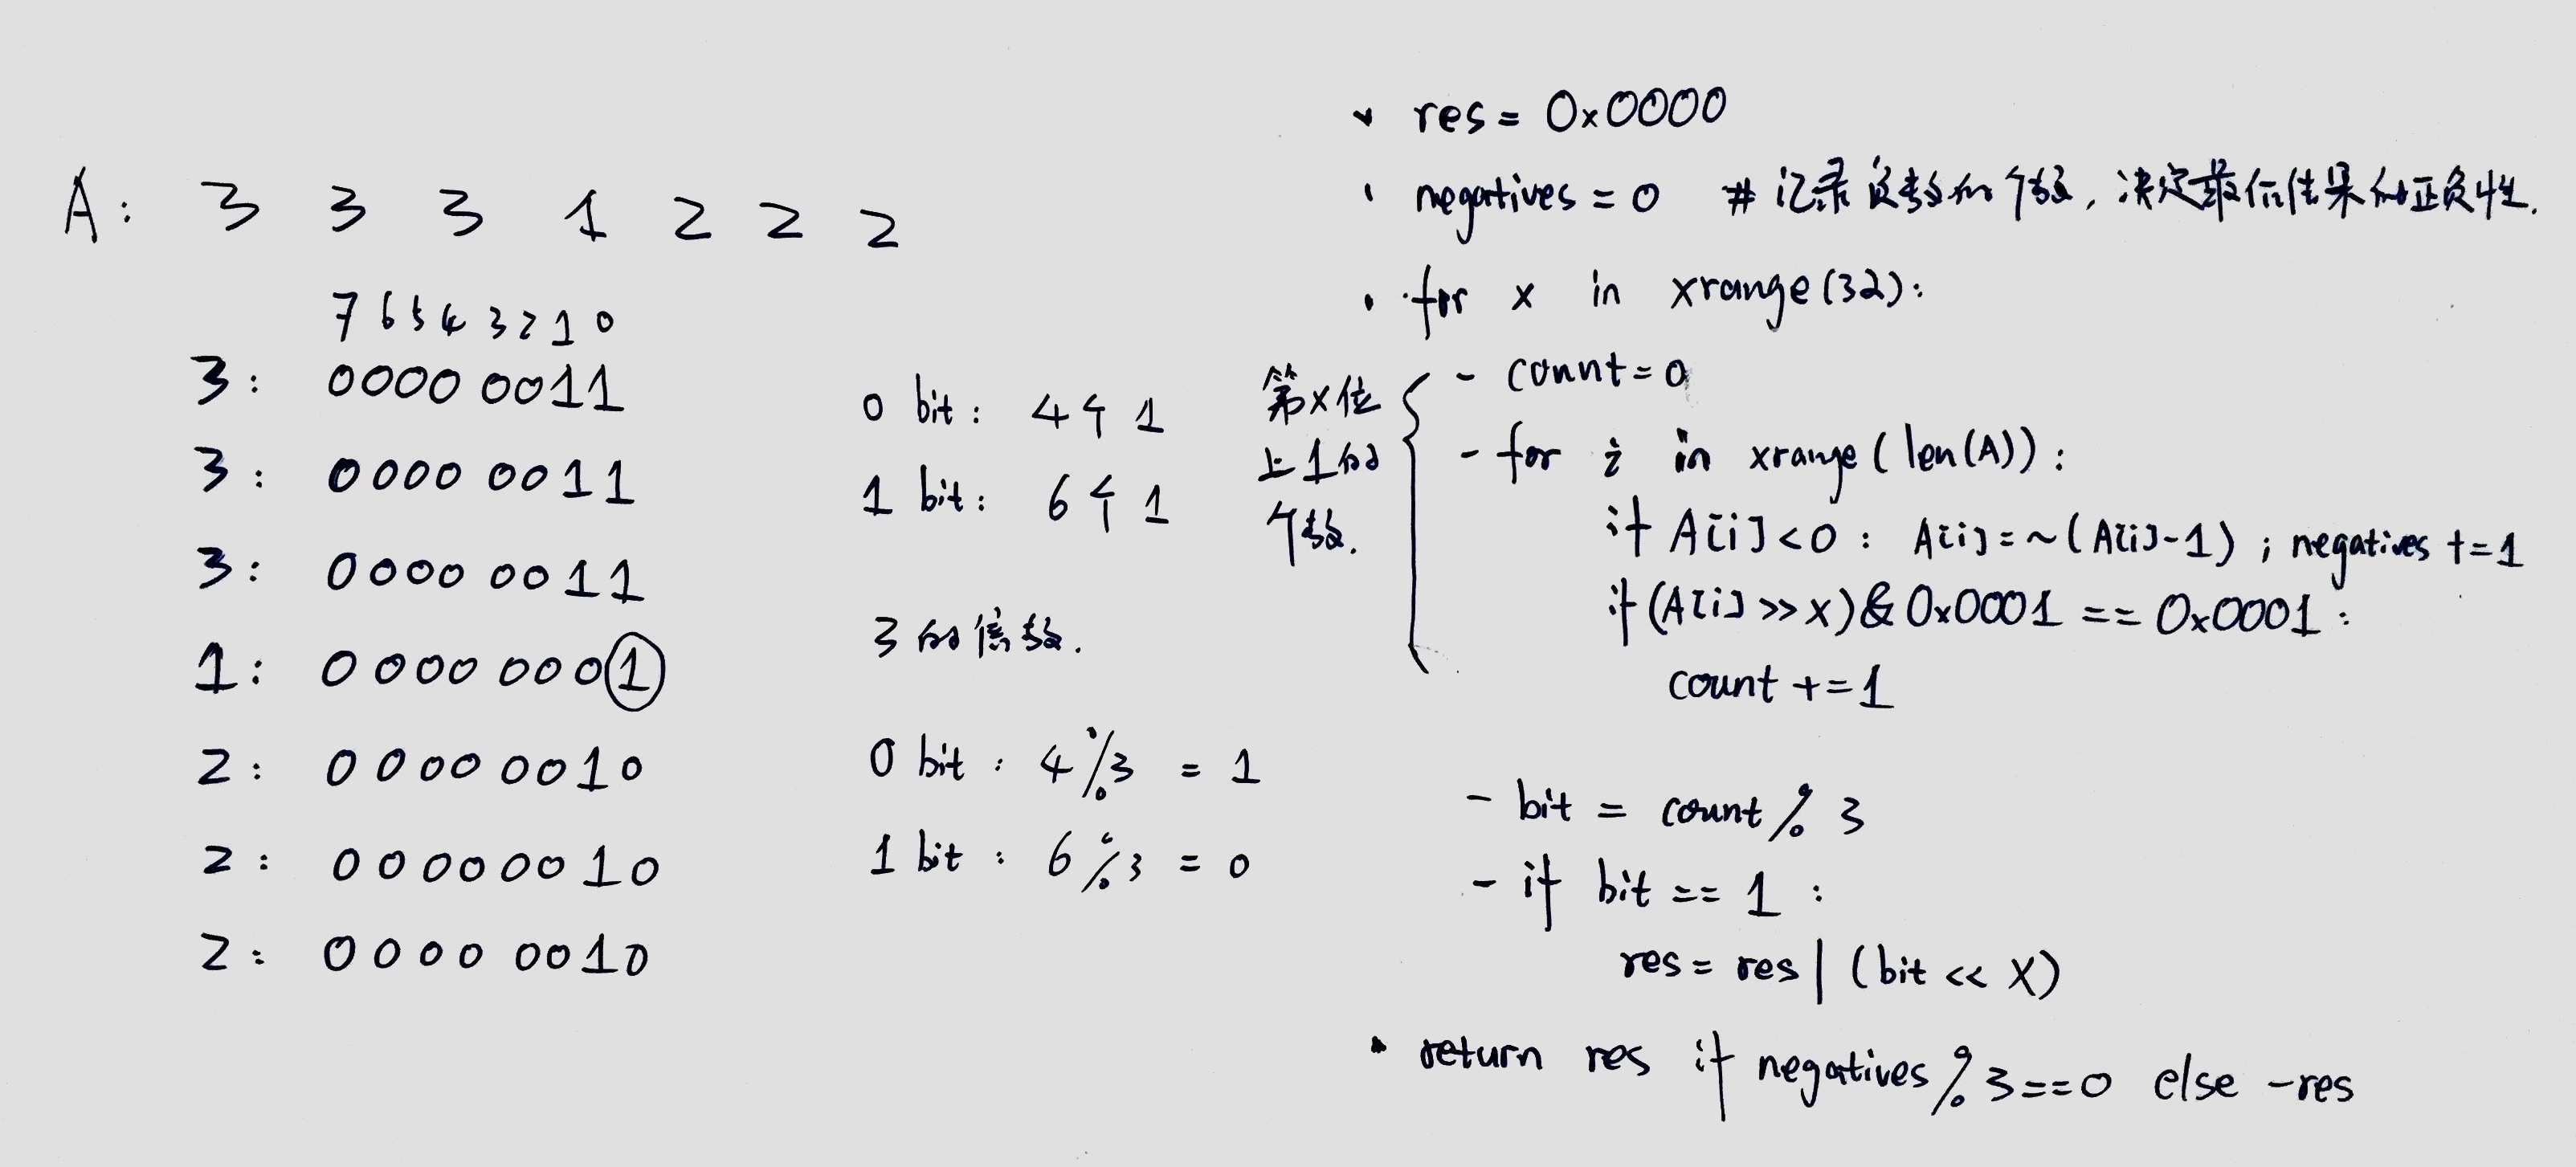
\includegraphics[width=\textwidth]{leetcode137.jpg}
    \centering \\
\end{figure}




\subsubsection{leetcode 126. Word Ladder II}
Given two words (beginWord and endWord), and a dictionary's word list, find all shortest transformation sequence(s) from beginWord to endWord, such that:
\begin{enumerate}
    \item Only one letter can be changed at a time
    \item Each intermediate word must exist in the word list
\end{enumerate}

\noindent For example, Given: beginWord = "hit", endWord = "cog", \\
wordList = ["hot","dot","dog","lot","log"], return
$$[["hit","hot","dot","dog","cog"],["hit","hot","lot","log","cog"]]$$ 
  
\noindent Note:
\begin{enumerate}
    \item All words have the same length.
    \item All words contain only lowercase alphabetic characters.
\end{enumerate}

\begin{CJK*}{UTF8}{gbsn}
\noindent 解题思路:
\begin{itemize}
    \item 创建一个用于查找直接前驱单词的字典prevMap,这个字典的key是单词表wordlist中的单词,value则是由这个单词的所有出现在字典中的前驱单词构成的列表。比如,prevMap=\{cog:[log,dog]\}表示cog的前驱是:log和dog。在每轮搜索过程中,根据搜索的结果更新相应的列表。
    \item 创建candidates[current]和candidates[previous]两个集合类型的数据结构,用于存储本轮搜索过程中找到的单词和前一轮搜索过程中找到的单词。采用集合类型的数据结构可以帮助去重。
    \item 搜索过程:
        \begin{enumerate}
            \item 在程序开始执行时,先将candidates[previous]中出现的单词从dict中删除,并且清空candidates[current];
            
            \item 然后遍历candidates[previous]中的单词,通过每次修改现有单词中的一个字母来寻找下一层的单词;如果修改后的单词在dict中,则将新单词存入candidates[current],同时更新前驱单词字典prevMap中相应的列表。例如,在下面示例图中,\{dot,lot\}的下一层为\{dog,log\},则将dog和log加入到candidates[current]中,同时更新prevMap[dot] 和 prevMap[lot]两个列表。
            
            \item 如果candidates[current]中出现了endWord,那么就说明转换路径已经找到,结束搜索的过程;如果candidates[current]中没有出现endWord,则将本轮搜索过程中得到的candidates[current]中的单词存入candidates [previous],然后重复上述搜索过程。
        \end{enumerate}
    \item 转换路径:路径的重建使用基于DFS算法就可以实现。
\end{itemize}
下面的示例图给出了分析过程及部分示例代码。图中的示例代码与下面给出的代码有些差别,但是都是基于同样的算法思想构建的。
\end{CJK*}

\begin{figure}[h]
    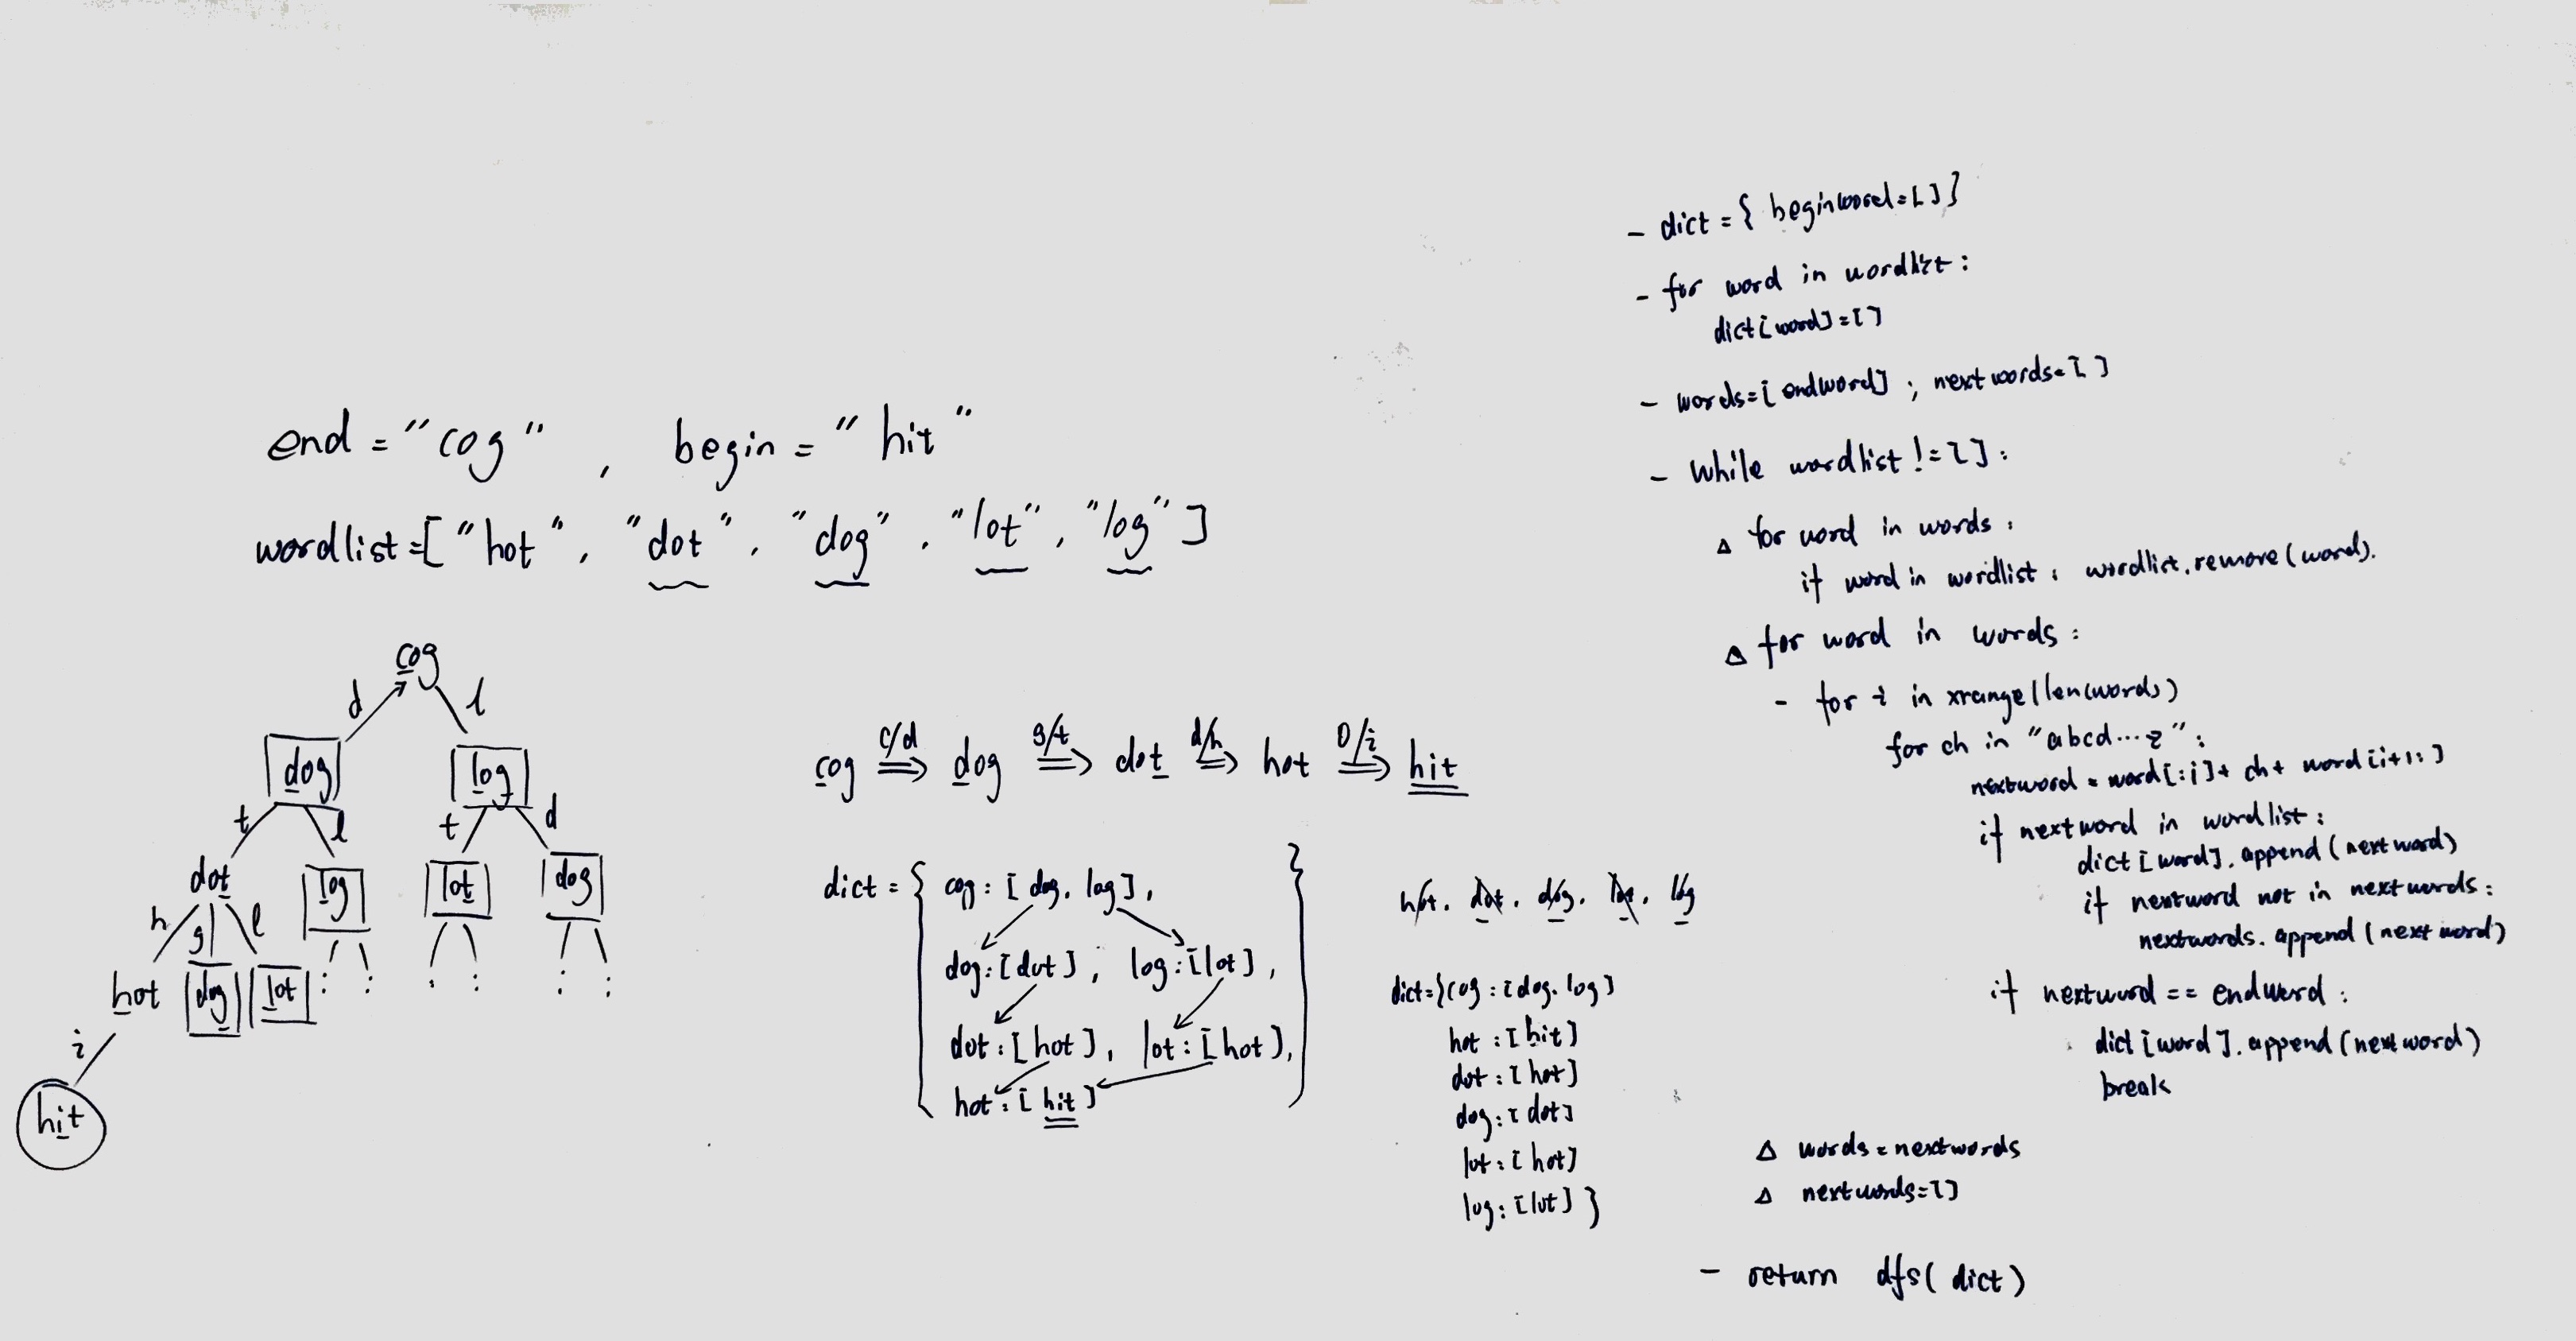
\includegraphics[width=\textwidth]{leetcode126.jpg}
    \centering \\
\end{figure}

\begin{lstlisting}[language=Python, caption=Problem126. Word Ladder II]

class Solution(object):
    def findLadders(self, beginWord, endWord, wordlist):
        """
        :type beginWord: str
        :type endWord: str
        :type wordlist: Set[str]
        :rtype: List[List[int]]
        """
        # do dfs to construct paths from beginWord to endWord
        # based on prevMap
        def dfsBuildPath(path, word):
            path.append(word)
            if len(prevMap[word])==0:
                currPath = path[:]
                currPath.reverse()
                res.append(currPath)
                return
            for w in prevMap[word]:
                dfsBuildPath(path, w)
                path.pop()

        res = []
        n = len(beginWord)
        prevMap = {}
        for word in wordlist:
            prevMap[word] = []
        
        # use two sets to simulate a queue by
        # switch them each round
        candidates = [set(), set()];
        current, previous = 0, 1
        candidates[current].add(beginWord)
        
        while True:
            current, previous = previous, current
            for word in candidates[previous]:
                wordlist.remove(word)
            candidates[current].clear()
            for word in candidates[previous]:
                # each time change one character in 'word'
                # if the new word exists in wordlist, save
                # it in prevMap and candidates' current set
                # for next round.
                for i in range(n):
                    part1=word[:i]; part2=word[i+1:]
                    for j in 'abcdefghijklmnopqrstuvwxyz':
                        if word[i]!=j:
                            nextword = part1 + j + part2
                            if nextword in wordlist:
                                prevMap[nextword].append(word)
                                candidates[current].add(nextword)
            # if no previous word exists in wordlist
            # it means beginWord cannot be transformed
            # into endWord
            if len(candidates[current])==0: return res
            if endWord in candidates[current]: break
        
        dfsBuildPath([], endWord)
        return res
\end{lstlisting}




\subsubsection{leetcode 54. Spiral Matrix}
Given a matrix of $m \times n$ elements ($m$ rows, $n$ columns), return all elements of the matrix in spiral order. For example, Given the following matrix:
    \begin{bmatrix}
       1 & 2 & 3 \\[0.3em]
       4 & 5 & 6 \\[0.3em]
       7 & 8 & 9
     \end{bmatrix}

\noindent You should return [1,2,3,6,9,8,7,4,5]. \\

\begin{CJK*}{UTF8}{gbsn}
\noindent 解题思路:螺旋遍历数组(从左向右,自上而下),一个比较直接的想法就是在每次遍历之前知道遍历的起点和终点,即每次遍历的矩阵的边界,我们可以用四个变量来记录每次遍历的边界值(上下左右):top, bottom, left, right。而每次遍历使用那一对儿边界值,可以通过每次遍历的方向(也是上下左右)来确定;同样我们有一个方向变量来记录每次遍历的方向,而且这个方向变量遵循一个规律就是先向右,再向下,然后向左,最后向上,这是一个遍历周期;下一个周期依然遵循同样的模式,直到整个矩阵遍历完。据此,我们可以通过对方向变量模除4的方式确定每次遍历的方向(代码line 29)。\\
\end{CJK*}

\begin{lstlisting}[language=Python, caption=Problem54. Spiral Matrix]

class Solution(object):
    def spiralOrder(self, matrix):
        res = []
        if matrix==[]: return res
        m, n = len(matrix), len(matrix[0])
        top, bottom = 0, m-1
        left, right = 0, n-1
        # direct indicates the direction of current move
        # 0:to right, 1:downwards, 2:to left, 3:upwards
        direct = 0
        while True:
            if direct==0:
                for y in xrange(left, right+1):
                    res.append(matrix[top][y])
                top += 1
            if direct==1:
                for x in xrange(top, bottom+1):
                    res.append(matrix[x][right])
                right -= 1
            if direct==2:
                for y in xrange(right, left-1, -1):
                    res.append(matrix[bottom][y])
                bottom -= 1
            if direct==3:
                for x in xrange(bottom, top-1, -1):
                    res.append(matrix[x][left])
                left += 1
            if top>bottom or left>right: return res
            direct = (direct+1)%4
\end{lstlisting}


\subsubsection{leetcode 59. Spiral Matrix II}
Given an integer $n$, generate a square matrix filled with elements from 1 to $n^2$ in spiral order. For example, Given $n = 3$, You should return the following matrix:
    \begin{bmatrix}
       1 & 2 & 3 \\[0.3em]
       8 & 9 & 4 \\[0.3em]
       7 & 6 & 5
     \end{bmatrix} \\

\begin{CJK*}{UTF8}{gbsn}
\noindent 解题思路:这道题是leetcode54. Spiral Matrix的逆过程,但是两题的相同点:本题填充矩阵的顺序即为leetcode54遍历矩阵的顺序。因此,算法在遍历数组的部分是完全相同的,差别在于while循环的结束条件(代码line30)。\\
\end{CJK*}

\begin{lstlisting}[language=Python, caption=Problem59. Spiral Matrix II]

class Solution(object):
    def generateMatrix(self, n):
        """
        :type n: int
        :rtype: List[List[int]]
        """
        if n == 0: return []
        matrix = [[0 for i in range(n)] for j in range(n)]
        top = 0; bottom = len(matrix)-1
        left = 0; right = len(matrix[0])-1
        direct = 0; count = 0
        while True:
            if direct == 0:
                for i in range(left, right+1):
                    count += 1; matrix[top][i] = count
                top += 1
            elif direct == 1:
                for i in range(top, bottom+1):
                    count += 1; matrix[i][right] = count
                right -= 1
            elif direct == 2:
                for i in range(right, left-1, -1):
                    count += 1; matrix[bottom][i] = count
                bottom -= 1
            elif direct == 3:
                for i in range(bottom, top-1, -1):
                    count += 1; matrix[i][left] = count
                left += 1
            if count == n*n: return matrix
            direct = (direct+1) % 4
\end{lstlisting}



\subsubsection{leetcode 238. Product of Array Except Self}
Given an array of $n$ integers where $n > 1$, nums, return an array output such that output[$i$] is equal to the product of all the elements of nums except nums[$i$]. Solve it \textbf{without division} and in O(n). For example, given [1,2,3,4], return [24,12,8,6]. \\

\noindent Follow up: Could you solve it with constant space complexity? (Note: The output array does not count as extra space for the purpose of space complexity analysis.) \\

\begin{CJK*}{UTF8}{gbsn}
\noindent 解题思路:根据题目对算法时间复杂度的要求, 设计一个两趟遍历的算法:
\begin{itemize}
    \item 第一趟正向遍历数组求各项的左积时,计算left_product[i]= nums[i-1]$\times$left_product[i-1],并且left_product[0]=1。
    \item 第二趟反向遍历数组求各项的右积时,计算right_product[i]=nums[i+1]$\times$right_product[i+1],并且right_product[n-1]=1。
    \item 最后的结果是计算res[i]=left_product[i]$\times$right_product[i]。
\end{itemize}
下面的示例图给出了具体的演算过程。\\
\end{CJK*}

\begin{lstlisting}[language=Python, caption=Problem238. Product of Array Except Self]

class Solution(object):
    def productExceptSelf(self, nums):
        """
        :type nums: List[int]
        :rtype: List[int]
        """
        n = len(nums)
        res = [1]*n
        product = 1
        for x in xrange(n-1):
            product *= nums[x]
            res[x+1] *= product
        product = 1
        for x in xrange(n-1, 0, -1):
            product *= nums[x]
            res[x-1] *= product
        return res
\end{lstlisting}

\begin{figure}[h]
    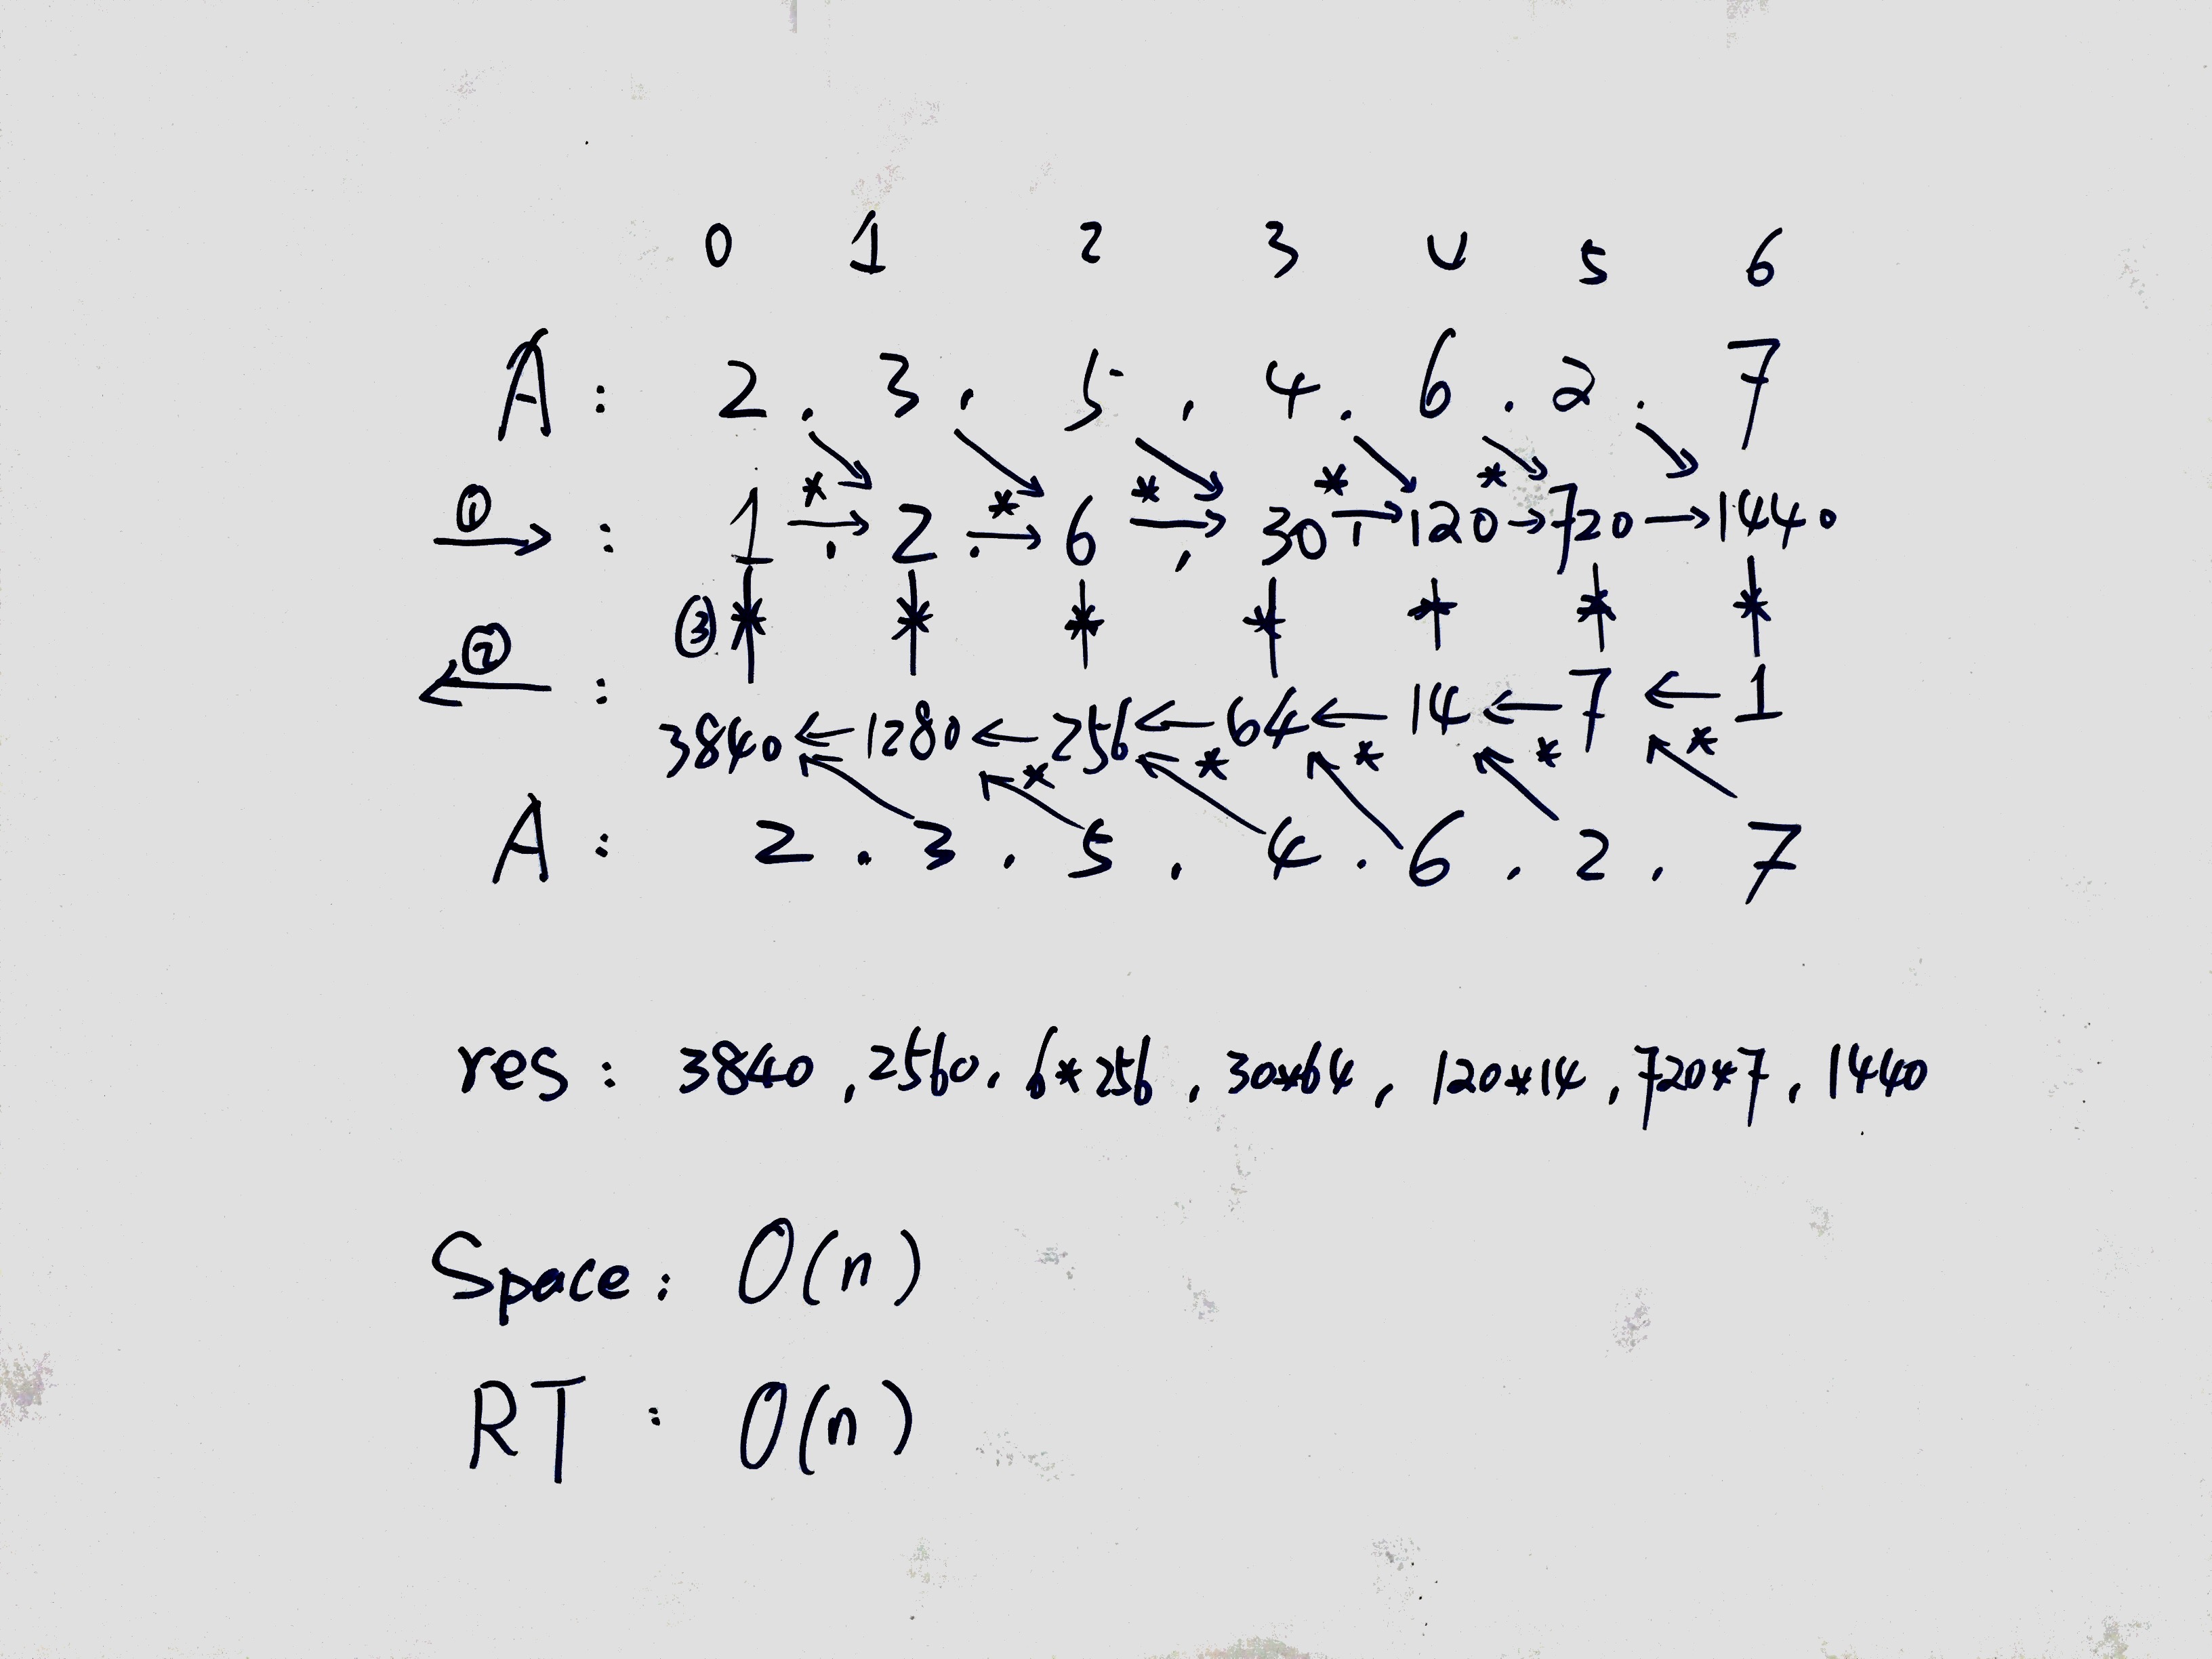
\includegraphics[width=\textwidth]{leetcode238.jpg}
    \centering \\
\end{figure}


\subsubsection{leetcode 268. Missing Number}
Given an array containing $n$ \textbf{distinct} numbers taken from 0, 1, 2, ..., n, find the one that is missing from the array. For example, Given nums = [0, 1, 3], return 2. \\

\noindent Note: Your algorithm should run in \textbf{linear runtime} complexity. Could you implement it using only \textbf{constant} extra space complexity? \\

\begin{CJK*}{UTF8}{gbsn}
\noindent 解题思路:这道题可以通过三种算法解决:
\begin{itemize}
    \item 第一种算法比较简单:因为题目中说明数组中的数值都是不同的,所以可以先对数组排序,然后依次比较前后两个数值的差是否为1:如果差值为1,说明相邻两数是连续的;如果差值不为1,说明已经找到missing number,返回即可。但是这个算法时间复杂度是$O(nlogn)$,不需要额外存储空间。
    \item 第二种算法是考虑数组是无序的,并且要在线性时间内求解,所以考虑使用hashtable的设计方法(在Python中用dict)。字典的(key,value)分别是数组中的元素和该元素对应的索引。在遍历数组构建字典dict的同时,可以记录序列中的最大值和最小值;然后以最小值为key,每次增1,依次查看key是否在字典dict中。如果不在,则返回当前key即可。这种算法的时间复杂度为$O(n)$,但空间复杂度为$O(n)$。
    \item 第三种算法的思想来自于leetcode136 Single Number。通过观察可以发现,长度为$n$的数组中数值的范围是[0..n],那么全部的索引值和所有值之间存在一种关系:缺失的值只在索引中出现过一次,而未缺失的值则在索引和数值中各出现一次,即出现两次,那么通过异或位运算,即可消除掉出现过两次的数值,最后剩下的即为缺失的数值。算法的时间复杂度是$O(n)$,空间复杂度是$O(1)$。
\end{itemize}
示例及演算过程见下面示例图。
\end{CJK*}

\begin{figure}[h]
    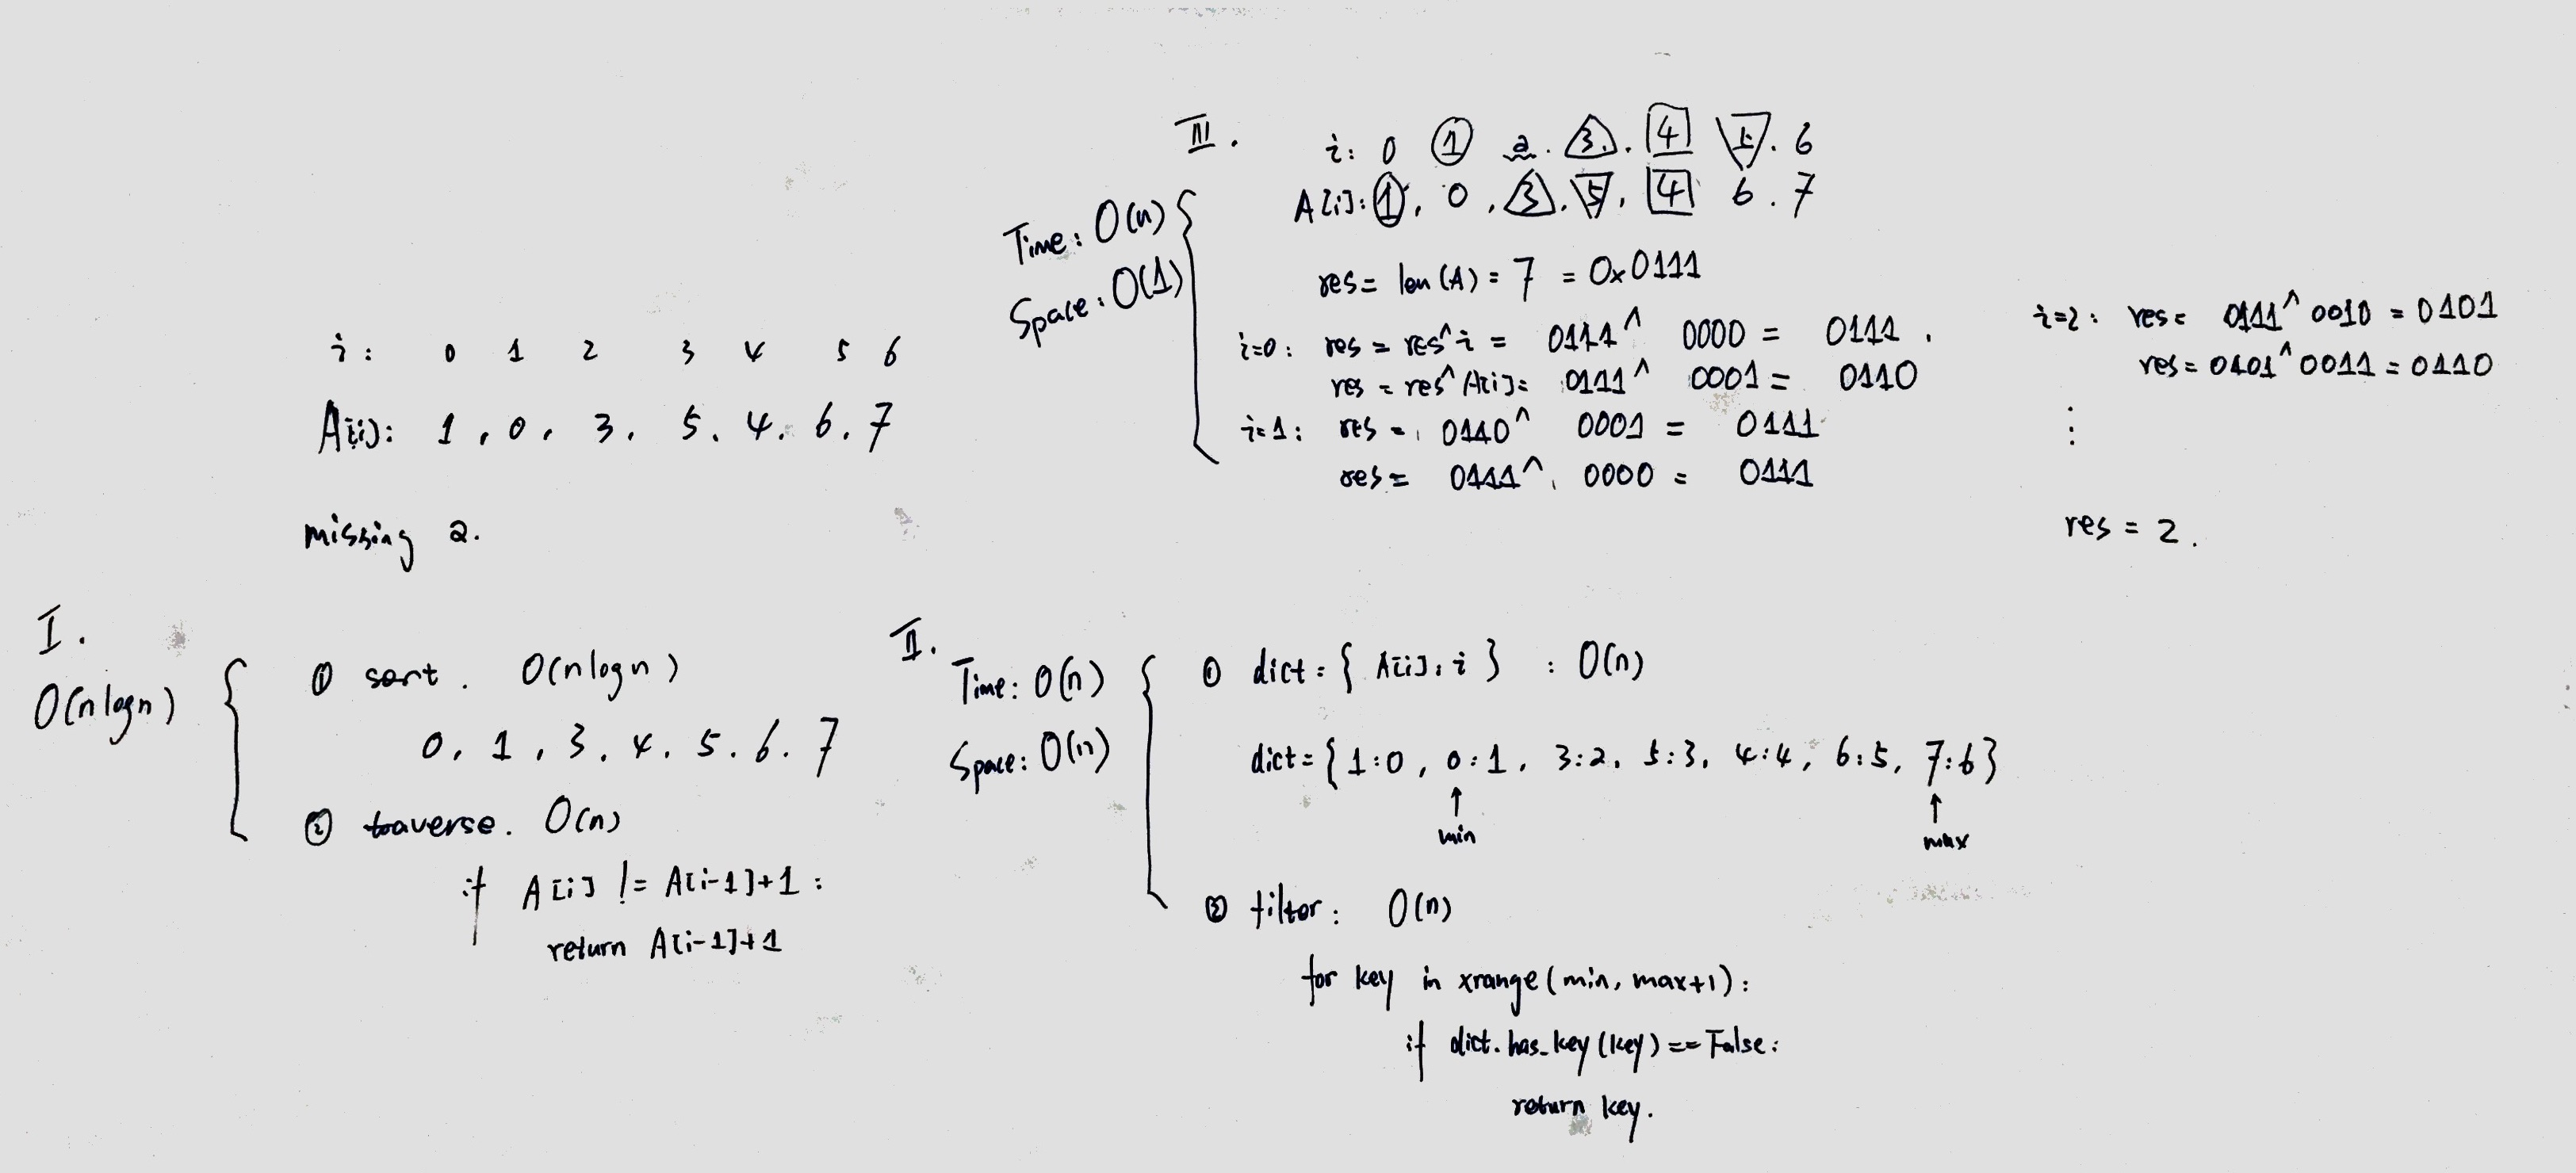
\includegraphics[width=\textwidth]{leetcode268.jpg}
    \centering \\
\end{figure}

\begin{lstlisting}[language=Python, caption=Problem268. Missing Number]

class Solution(object):
    def missingNumber(self, nums): # RT: O(n)
        """
        :type nums: List[int]
        :rtype: int
        """
        res = len(nums)
        for i in xrange(len(nums)):
            res = res^i
            res = res^nums[i]
        return res
\end{lstlisting}


\subsubsection{leetcode 209. Minimum Size Subarray Sum}
Given an array of $n$ positive integers and a positive integer $s$, find the \textbf{minimal length} of a subarray of which the sum $\geq s$. If there isn't one, return 0 instead. \\

\noindent For example, given the array [2,3,1,2,4,3] and s = 7, the subarray [4,3] has the minimal length under the problem constraint. \\

\noindent More practice: If you have figured out the O(n) solution, try coding another solution of which the time complexity is O(n log n). \\

\begin{CJK*}{UTF8}{gbsn}
\noindent 解题思路:开辟一个窗口,通过滑动窗口的左右边界,取得满足条件的最小窗口大小即为最小子数组的长度。滑动窗口的条件是:如果当前窗口内所有数值的和小于目标值,移动窗口右边界,向当前窗口内增加一个数值;如果当前窗口内所有数值的和大于或等于目标值,移动窗口的左边界,将当前窗口最左侧的数值移除窗口。上述过程的结束条件就是窗口右边界达到数组边界。参考下面的示例图。
\end{CJK*}

\begin{figure}[h]
    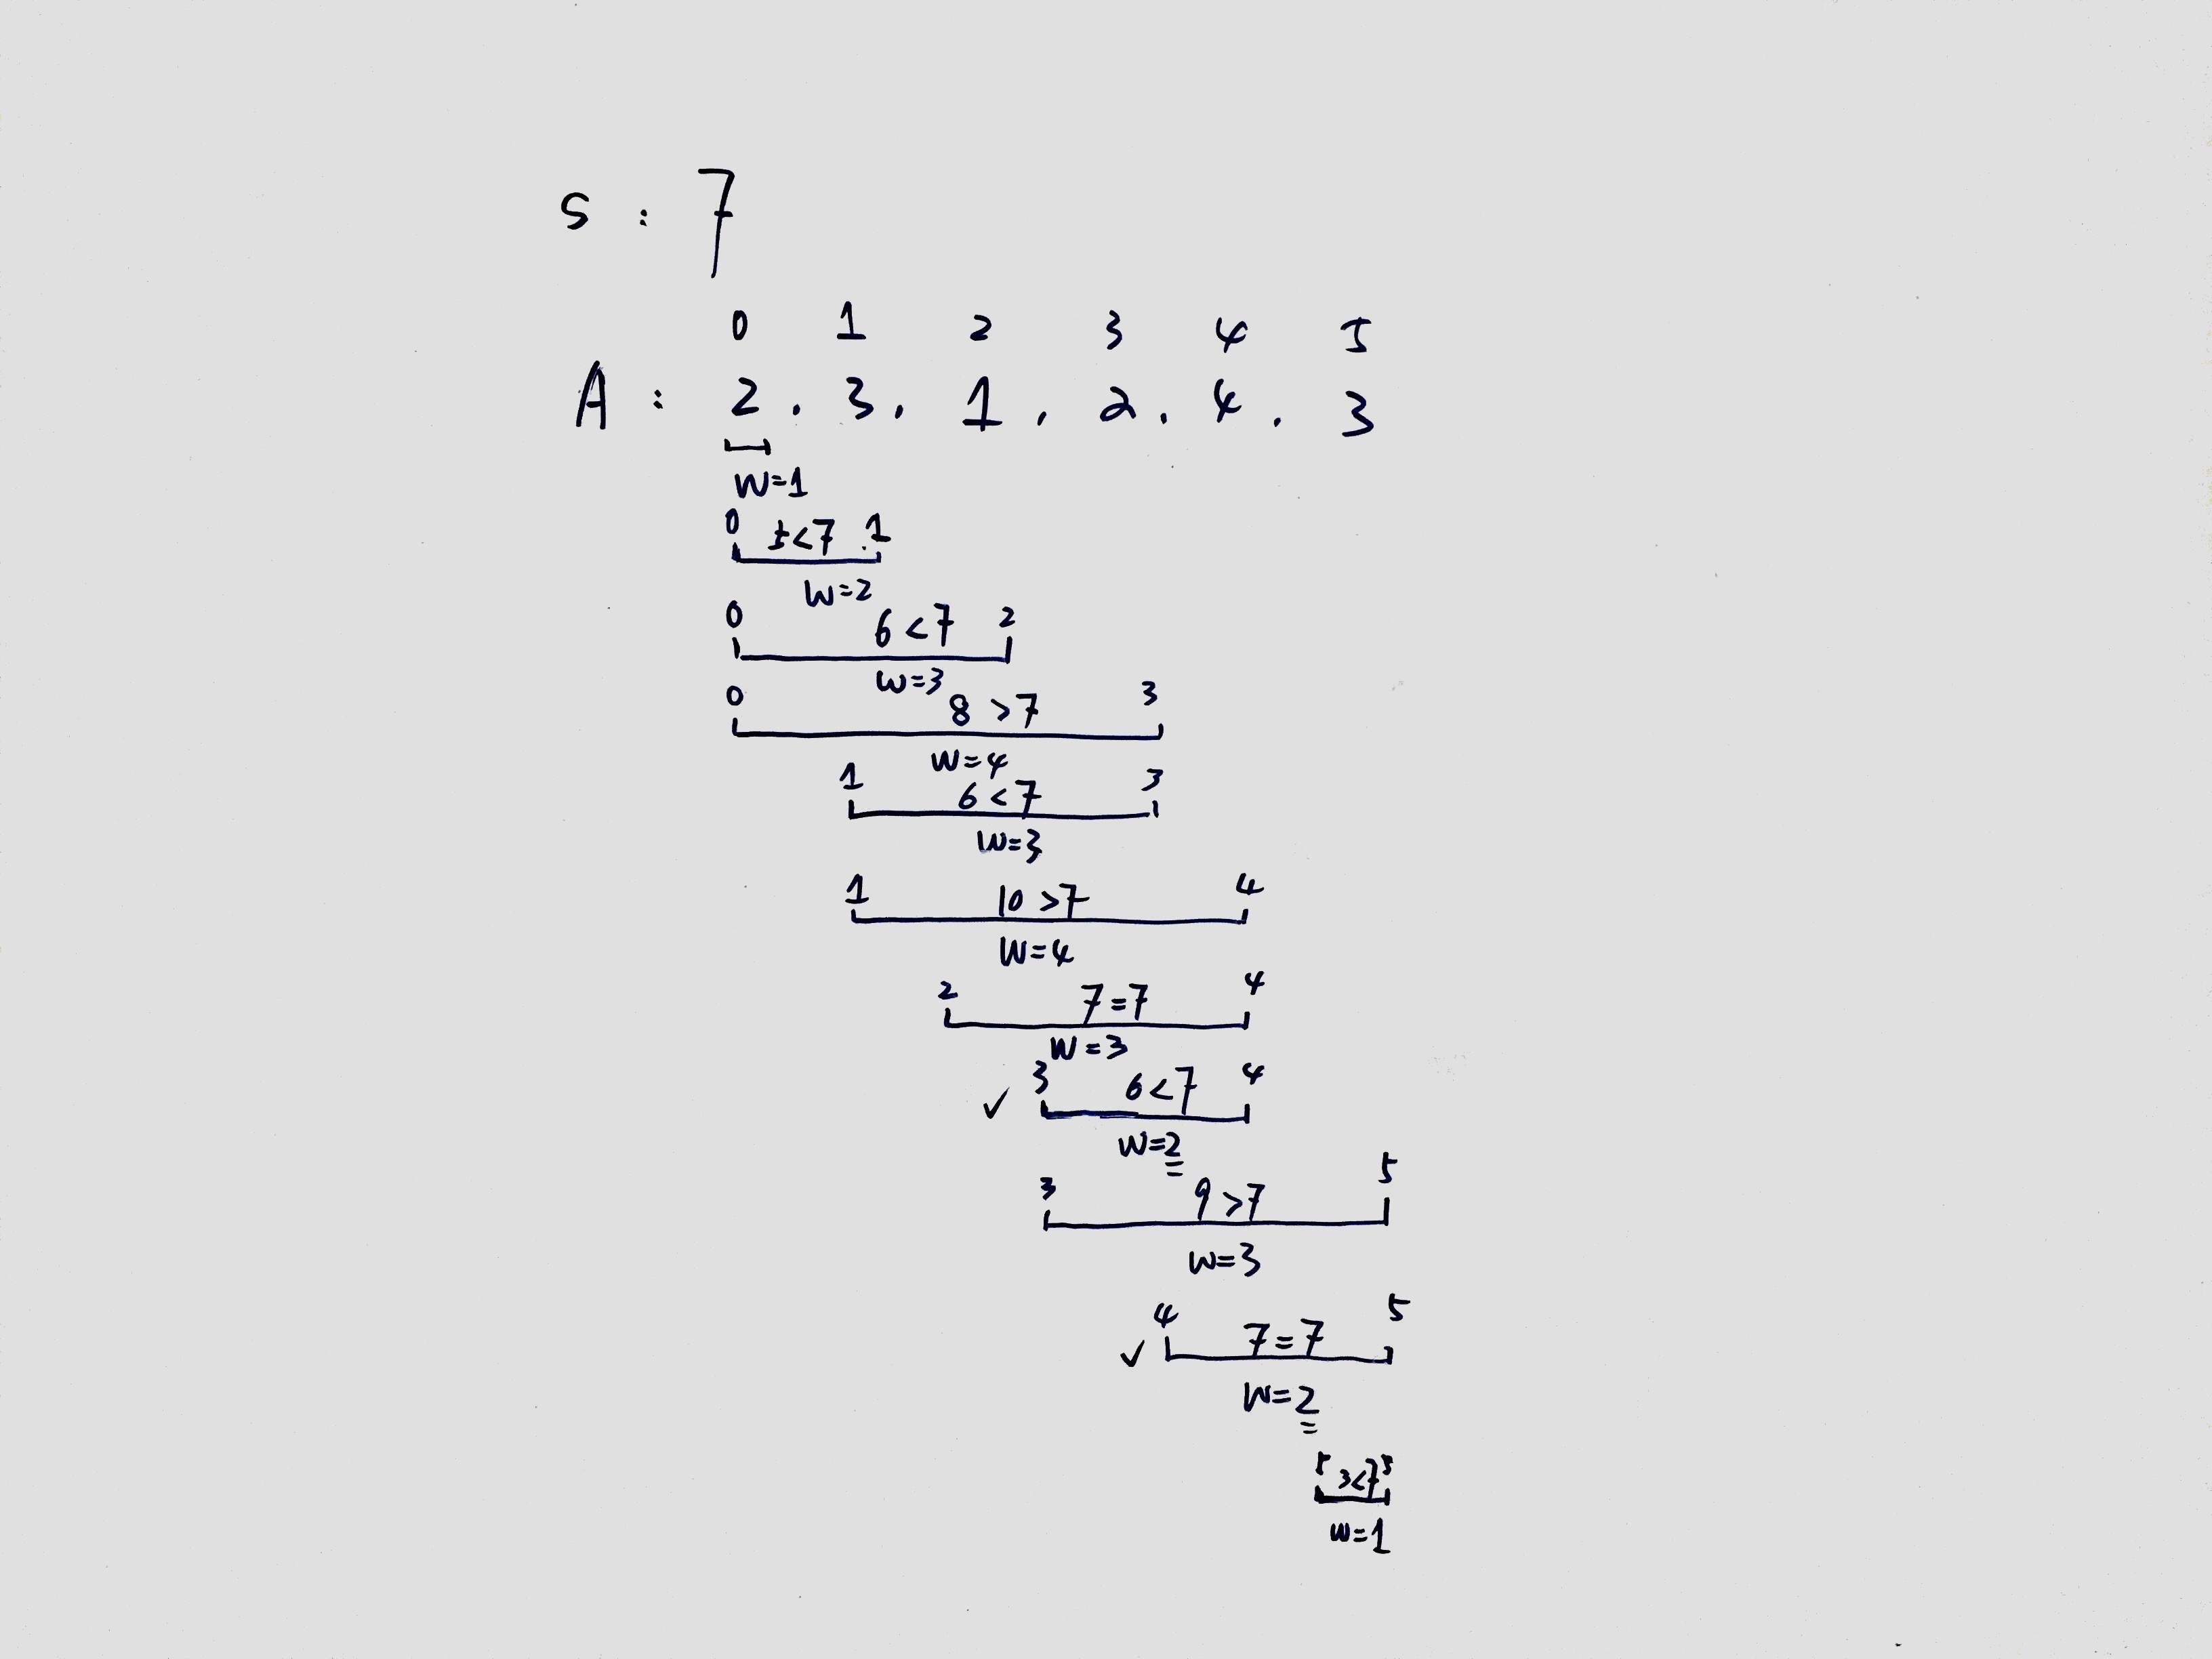
\includegraphics[width=10cm]{leetcode209.jpg}
    \centering \\
\end{figure}

\begin{lstlisting}[language=Python, caption=Problem209. Minimum Size Subarray Sum]

class Solution(object):
    def minSubArrayLen(self, s, nums): # RT: O(n)
        """
        :type s: int
        :type nums: List[int]
        :rtype: int
        """
        size = len(nums)
        left, right, sum = 0, 0, 0
        window = size + 1
        while right < size:
            # increase window
            while right < size and sum < s:
                sum += nums[right]
                right += 1
            # decrease window
            while left < right and sum >= s:
                window = min(window, right - left)
                sum -= nums[left]
                left += 1
        return window if window <= size else 0
\end{lstlisting}


\subsubsection{leetcode 56. Merge Intervals}
Given a collection of intervals, merge all overlapping intervals. For example, Given [1,3],[2,6],[8,10],[15,18], return [1,6],[8,10],[15,18]. \\

\begin{CJK*}{UTF8}{gbsn}
\noindent 解题思路:因为给定的一组区间可能是无序的,所以首先按照start的值对区间进行排序(从小到大);然后比较当前区间的end与下一个区间的start的大小,如果两区间存在重叠,那么就合并这两个区间;否则下一个区间变为当前区间,重复上述过程。参考下面的示例图。
\end{CJK*}

\begin{figure}[h]
    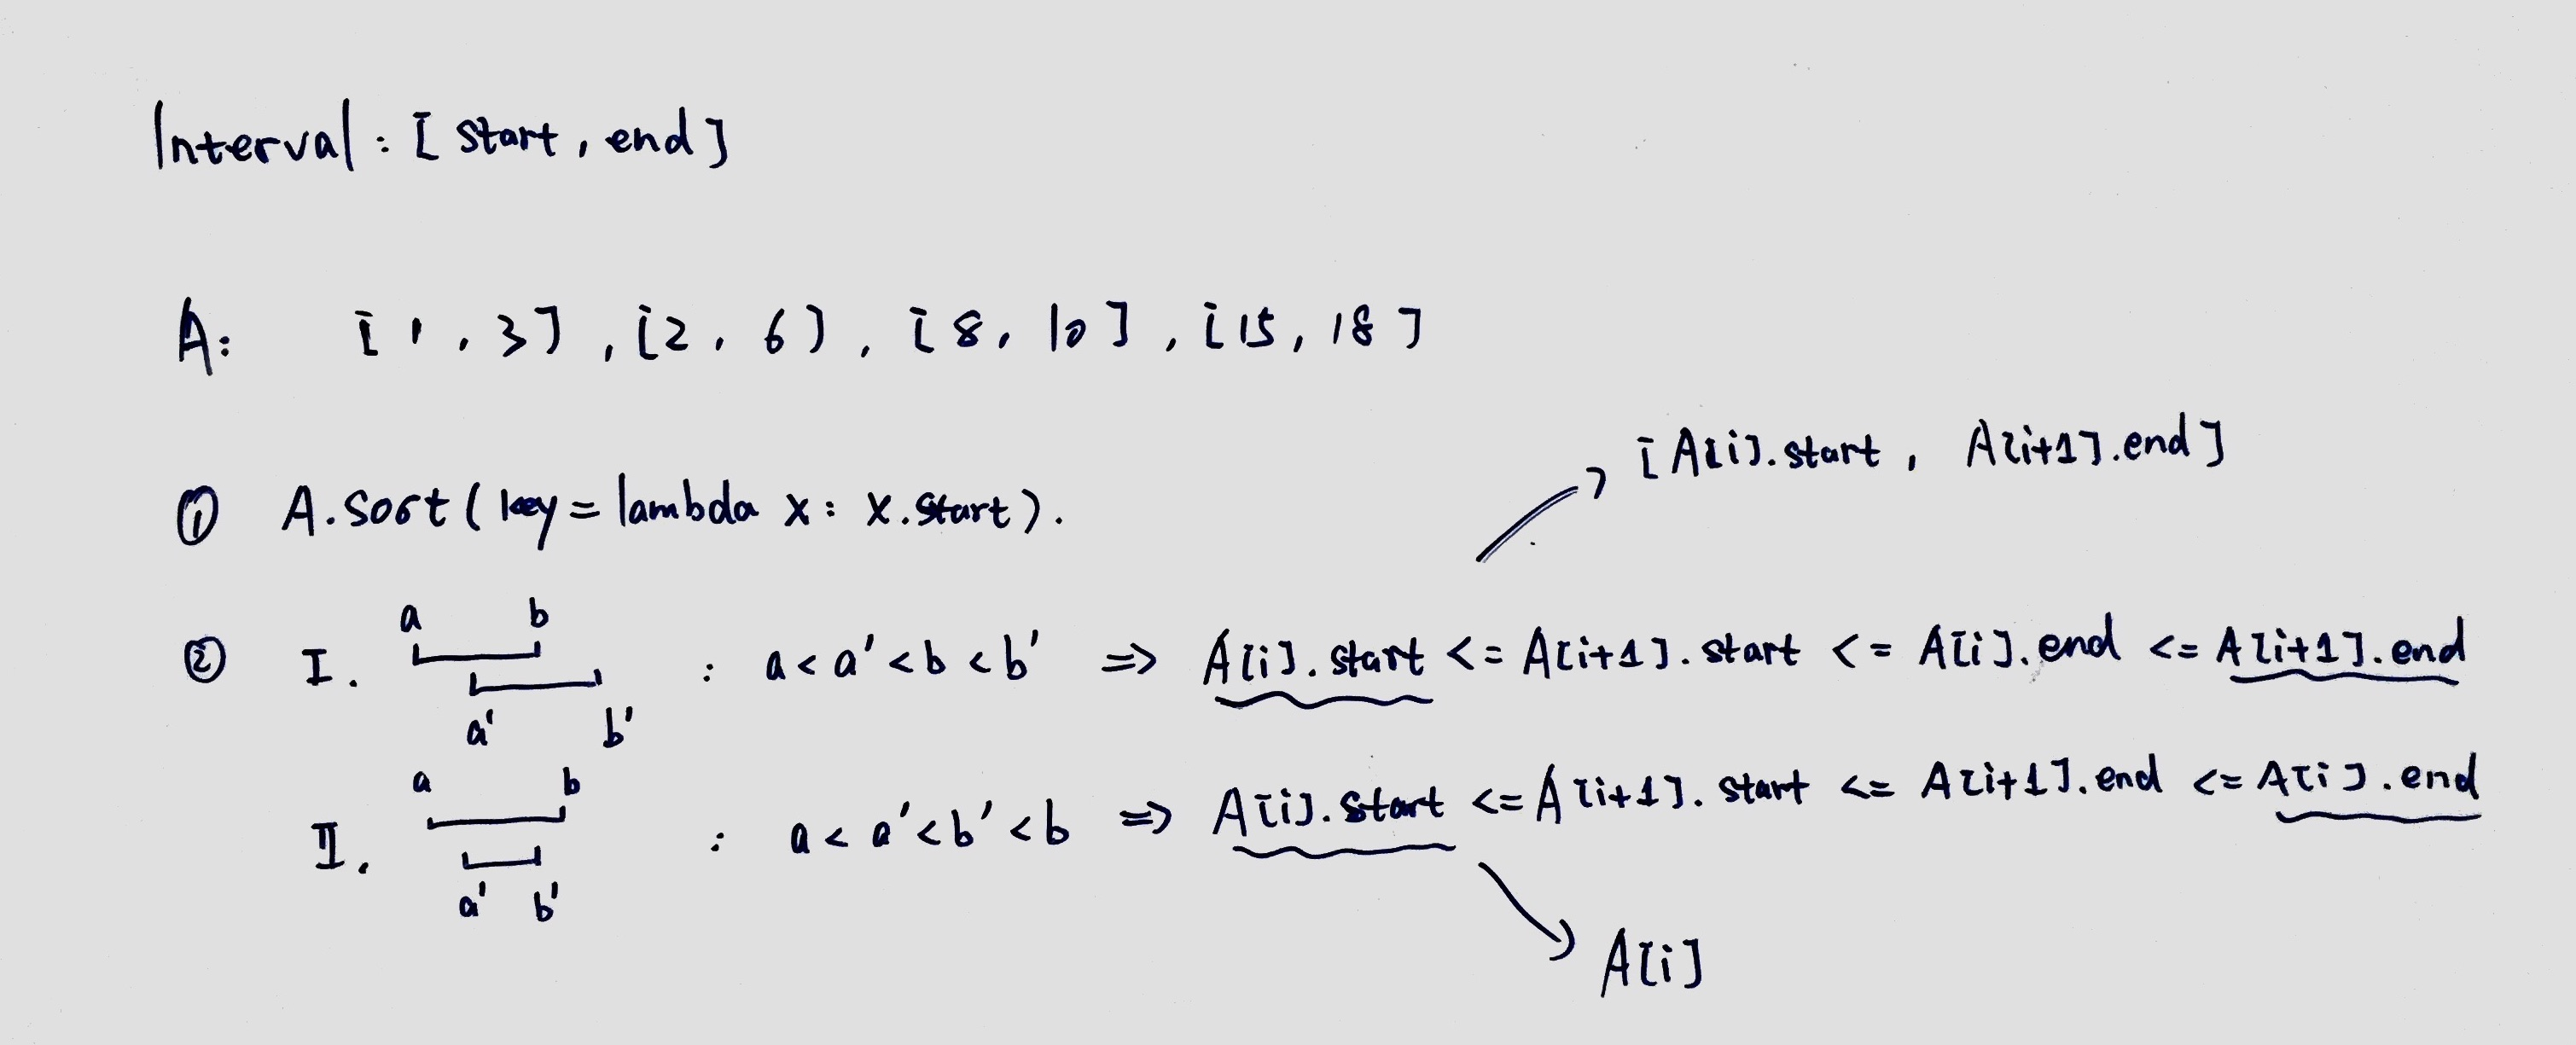
\includegraphics[width=\textwidth]{leetcode56.jpg}
    \centering \\
\end{figure}

\begin{lstlisting}[language=Python, caption=Problem56. Merge Intervals]

# Definition for an interval.
# class Interval(object):
#     def __init__(self, s=0, e=0):
#         self.start = s
#         self.end = e

class Solution(object):
    def merge(self, intervals):  # O(n) time
        """
        :type intervals: List[Interval]
        :rtype: List[Interval]
        """
        intervals.sort(key=lambda x:x.start)
        m = len(intervals)
        res = []
        if m==0: return res
        curr = intervals[0]
        for x in range(1, m):
            if intervals[x].start <= curr.end:
                curr.end = max(curr.end, intervals[x].end)
            else:
                res.append(curr)
                curr = intervals[x]
        res.append(curr)
        return res
\end{lstlisting}


\subsubsection{leetcode 229. Majority Element II}
Given an integer array of size $n$, find all elements that appear more than $\lfloor n/3 \rfloor$ times. The algorithm should run in \textbf{linear} time and in \textbf{O(1) space}. \\

\begin{CJK*}{UTF8}{gbsn}
\noindent 解题思路:题目要求在线性时间内求解,所以算法的设计一定不会使用到排序。在线性时间内求解无序数组的某种性质的问题,可以考虑使用hashtable。但是,这倒题目对空间复杂度的要求是O(1),基于hashtable的算法是无法满足的。这道题题目求解的是众数问题,需要基于Boyer–Moore majority vote算法进行设计。算法的思想基本与BM算法一致,分为两个阶段:
\begin{itemize}
    \item 第一个阶段求出候选的众数。根据题目的要求,在给定的数组中,出现次数超过$\lfloor n/3 \rfloor$次的元素的个数最多有两个。可以通过一次遍历给定的数组,找到出现次数最多的两个元素。
    \item 第二阶段是验证两个候选元素是否出现的次数满足题目的要求,即出现次数多于$\lfloor n/3 \rfloor$。
\end{itemize}
\noindent这个算法可以在$O(n)$时间内完成,同时满足题目对空间复杂度的要求$O(1)$。
\end{itemize}
参见下面示例图中的分析和演算。
\end{CJK*}

\begin{figure}[h]
    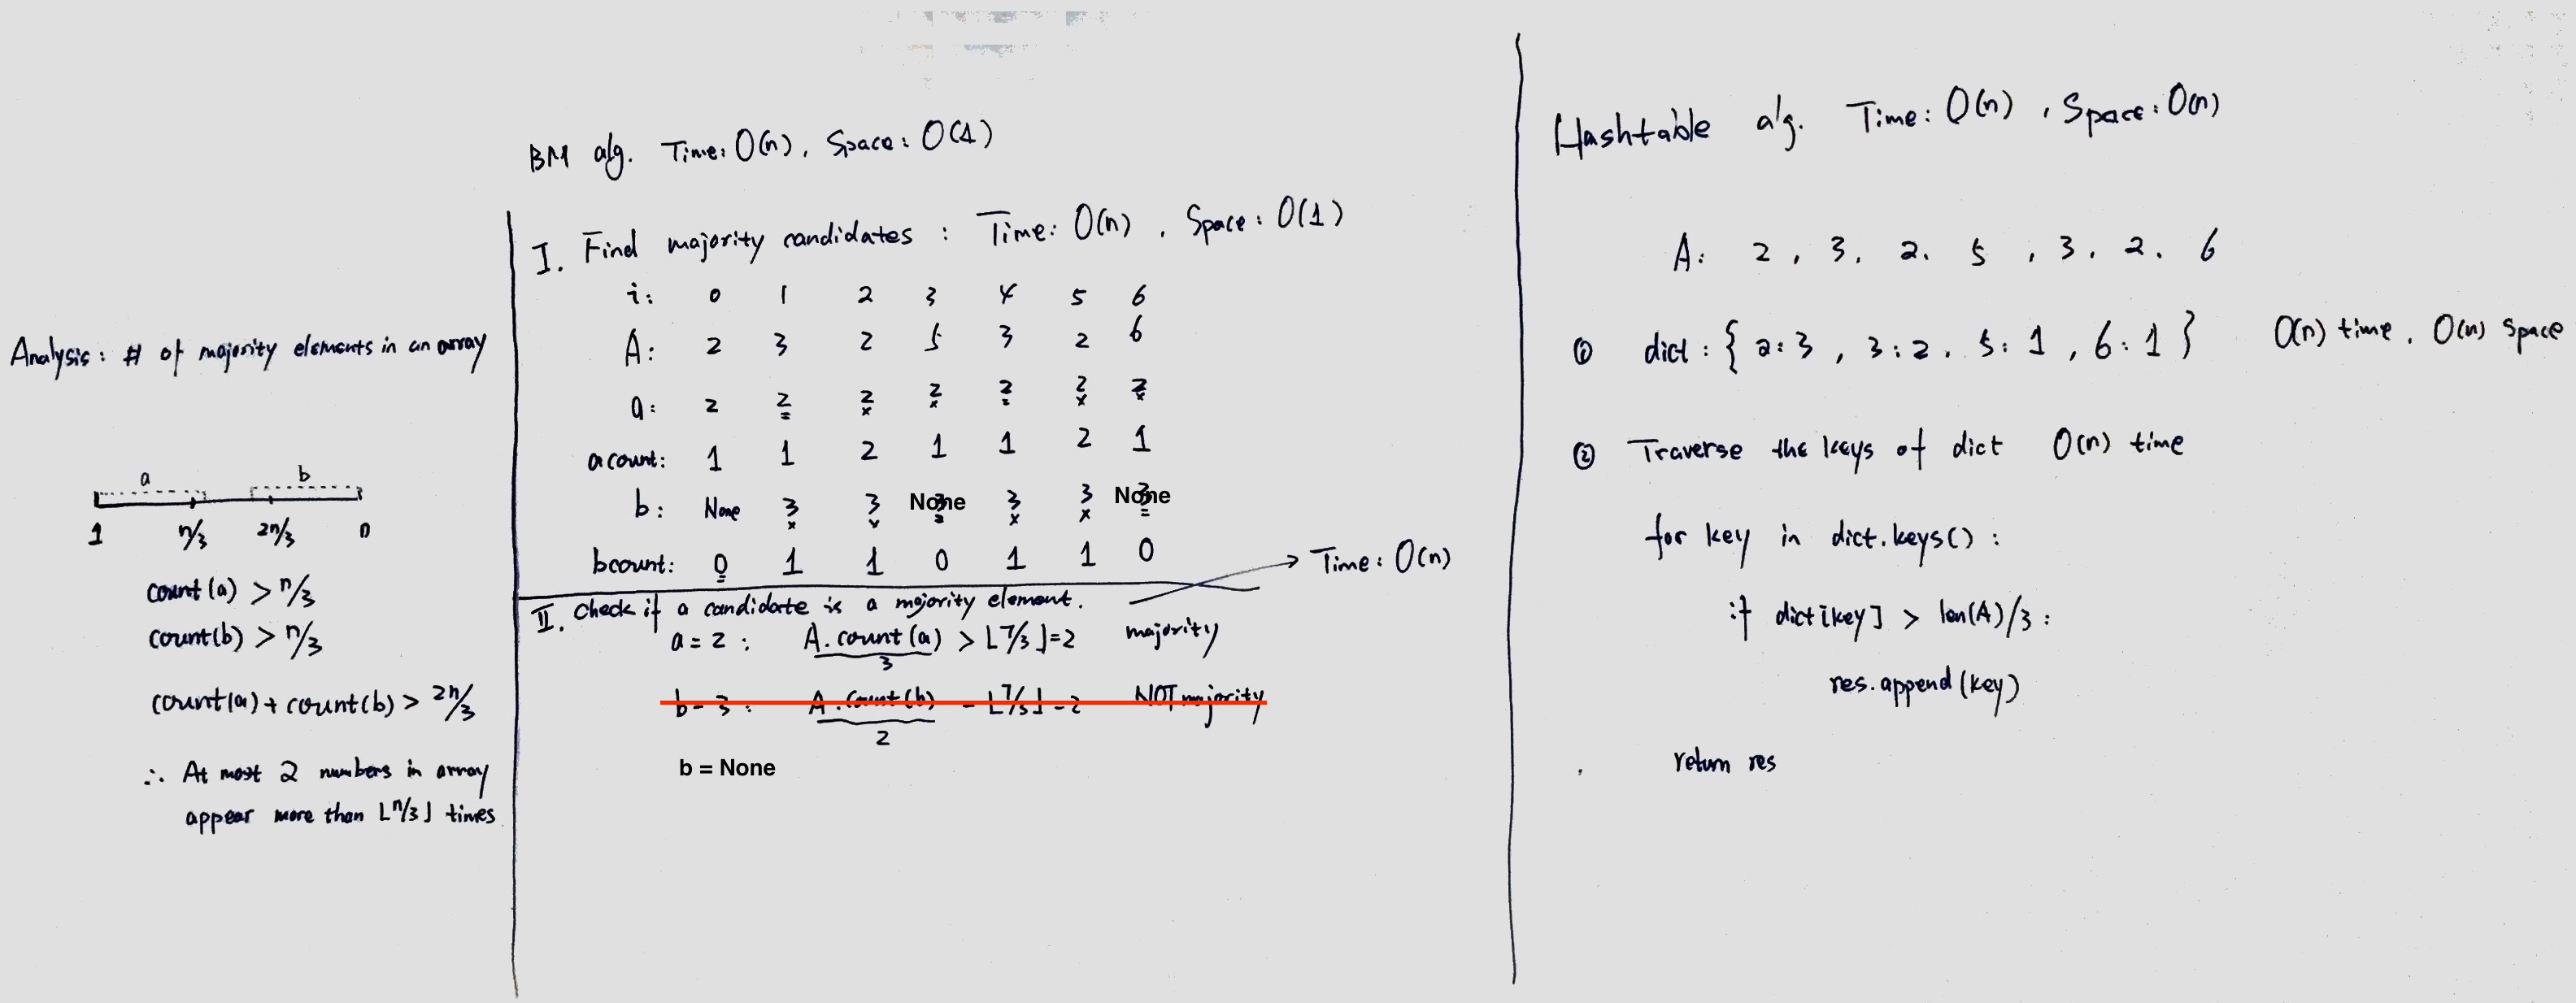
\includegraphics[width=\textwidth]{leetcode229.jpg}
    \centering \\
\end{figure}

\begin{lstlisting}[language=Python, caption=Problem229. Majority Element II]

class Solution(object):
    def majorityElement_dict(self, nums): # RT: O(n), Space: O(n)
        dict = {}
        for num in nums:
            if dict.has_key(num)==False:
                dict[num] = 1
            else:
                dict[num] += 1
        res = []
        for key in dict.keys():
            if dict[key] > len(nums)/3:
                res.append(key)
        return res
        
    def majorityElement_BM(self, nums): # RT: O(n), Space: O(1)
        """
        :type nums: List[int]
        :rtype: List[int]
        """
        n = len(nums)
        candidate1, count1 = None, 0
        candidate2, count2 = None, 0
        for num in nums:
            if num == candidate1: count1 += 1
            elif num == candidate2: count2 += 1
            elif count1 == 0: candidate1, count1 = num, 1
            elif count2 == 0: candidate2, count2 = num, 1
            else: count1 -= 1; count2 -= 1
        return [x for x in (candidate1, candidate2) if nums.count(x) > n/3]
\end{lstlisting}


\subsubsection{leetcode 55. Jump Game}
Given an array of non-negative integers, you are initially positioned at the first index of the array. Each element in the array represents your maximum jump length at that position. Determine if you are able to reach the last index. \\

\noindent For example:
\begin{enumerate}
    \item A = [2,3,1,1,4], return true.
    \item A = [3,2,1,0,4], return false.
\end{enumerate}

\begin{CJK*}{UTF8}{gbsn}
\noindent 解题思路:这道题可以用决策树也可以用贪心算法。但是,决策树会超时。贪心算法是从起点开始,每向前走一步,就比较当前位置可以走的步数和剩余可走步数的大小,每次取两者的最大值。如此进行下去,如果在迭代结束之前,可走的最大步数为0,说明没法走到数组的末端。两种算法的示例和演算见下图。
\end{CJK*}

\begin{figure}[h]
    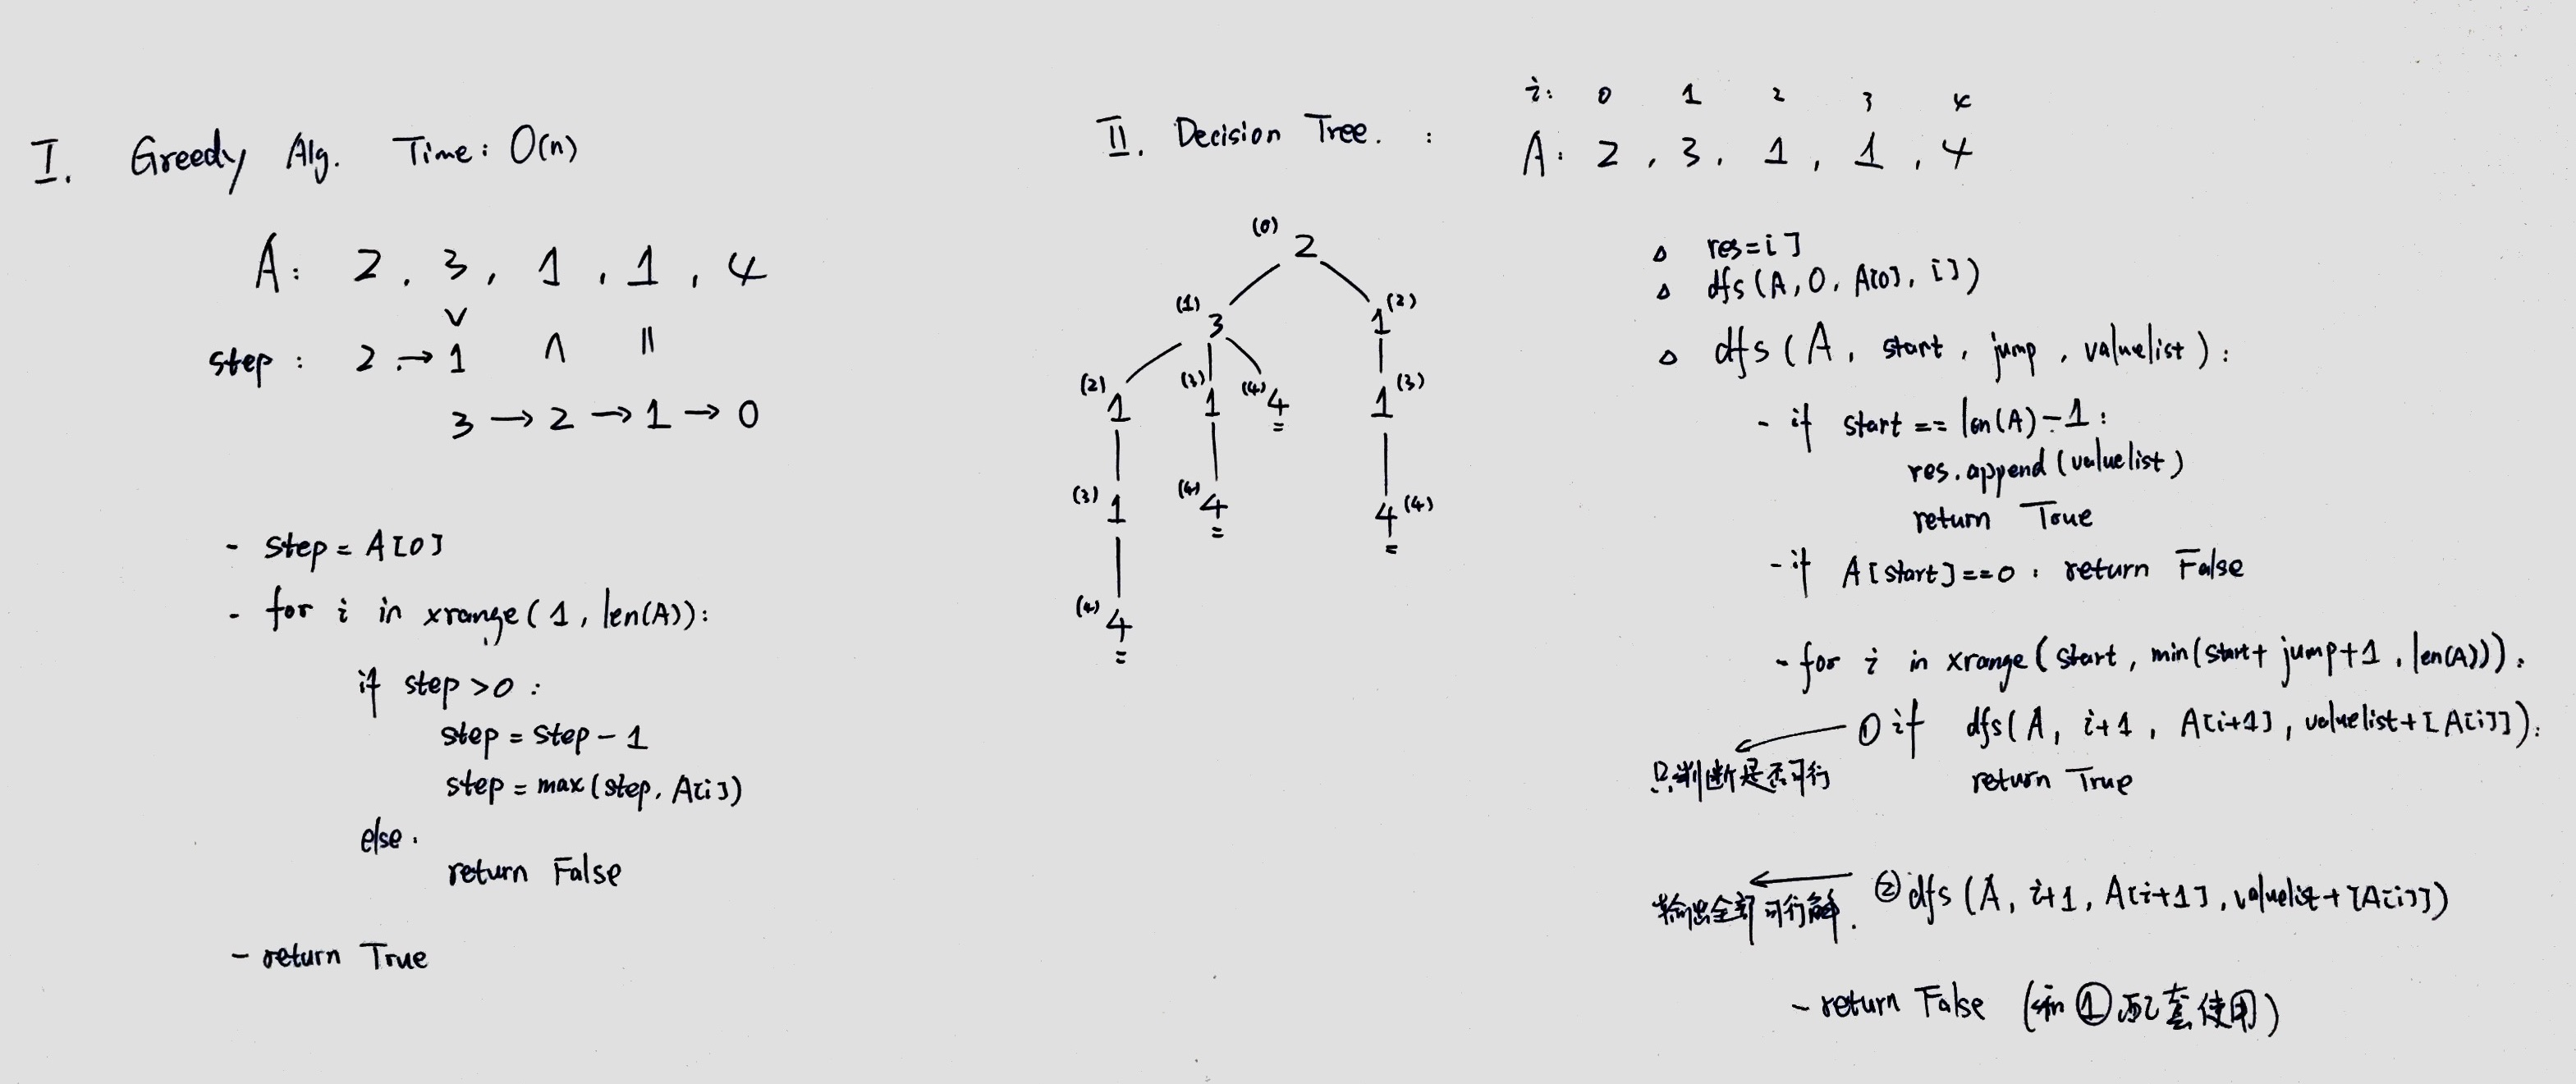
\includegraphics[width=\textwidth]{leetcode55.jpg}
    \centering \\
\end{figure}

\begin{lstlisting}[language=Python, caption=Problem55. Jump Game]

class Solution(object):
    def canJump(self, nums):
        """
        :type nums: List[int]
        :rtype: bool
        """
        step = nums[0]
        for i in range(1, len(nums)):
            if step > 0:
                step -= 1
                step = max(step, nums[i])
            else:
                return False
        return True
\end{lstlisting}


\subsubsection{leetcode 45. Jump Game II}
Given an array of \textbf{non-negative} integers, you are initially positioned at the first index of the array. Each element in the array represents your maximum jump length at that position. Your goal is to reach the last index in the \textbf{minimum} number of jumps. \\

\noindent For example: Given array A = [2,3,1,1,4]. The minimum number of jumps to reach the last index is 2. (Jump 1 step from index 0 to 1, then 3 steps to the last index.) \\

\noindent Note: You can assume that you can always reach the last index.

\begin{CJK*}{UTF8}{gbsn}
\noindent 这道题的解题思路见示例图右侧部分。示例图左侧为具体示例。

\noindent 代码说明:用lastCanReach记录jumpNum次跳跃后,所能够到达的最大索引值;用currCanReach记录在lastCanReach的范围内所有索引能够到达的最大索引值。如果当前遍历的索引值超过了lastCanReach的范围,则用currCanReach更新lastCanReach,这也意味着需要多跳跃一次,即jumpNum增1。
\end{CJK*}

\begin{figure}[h]
    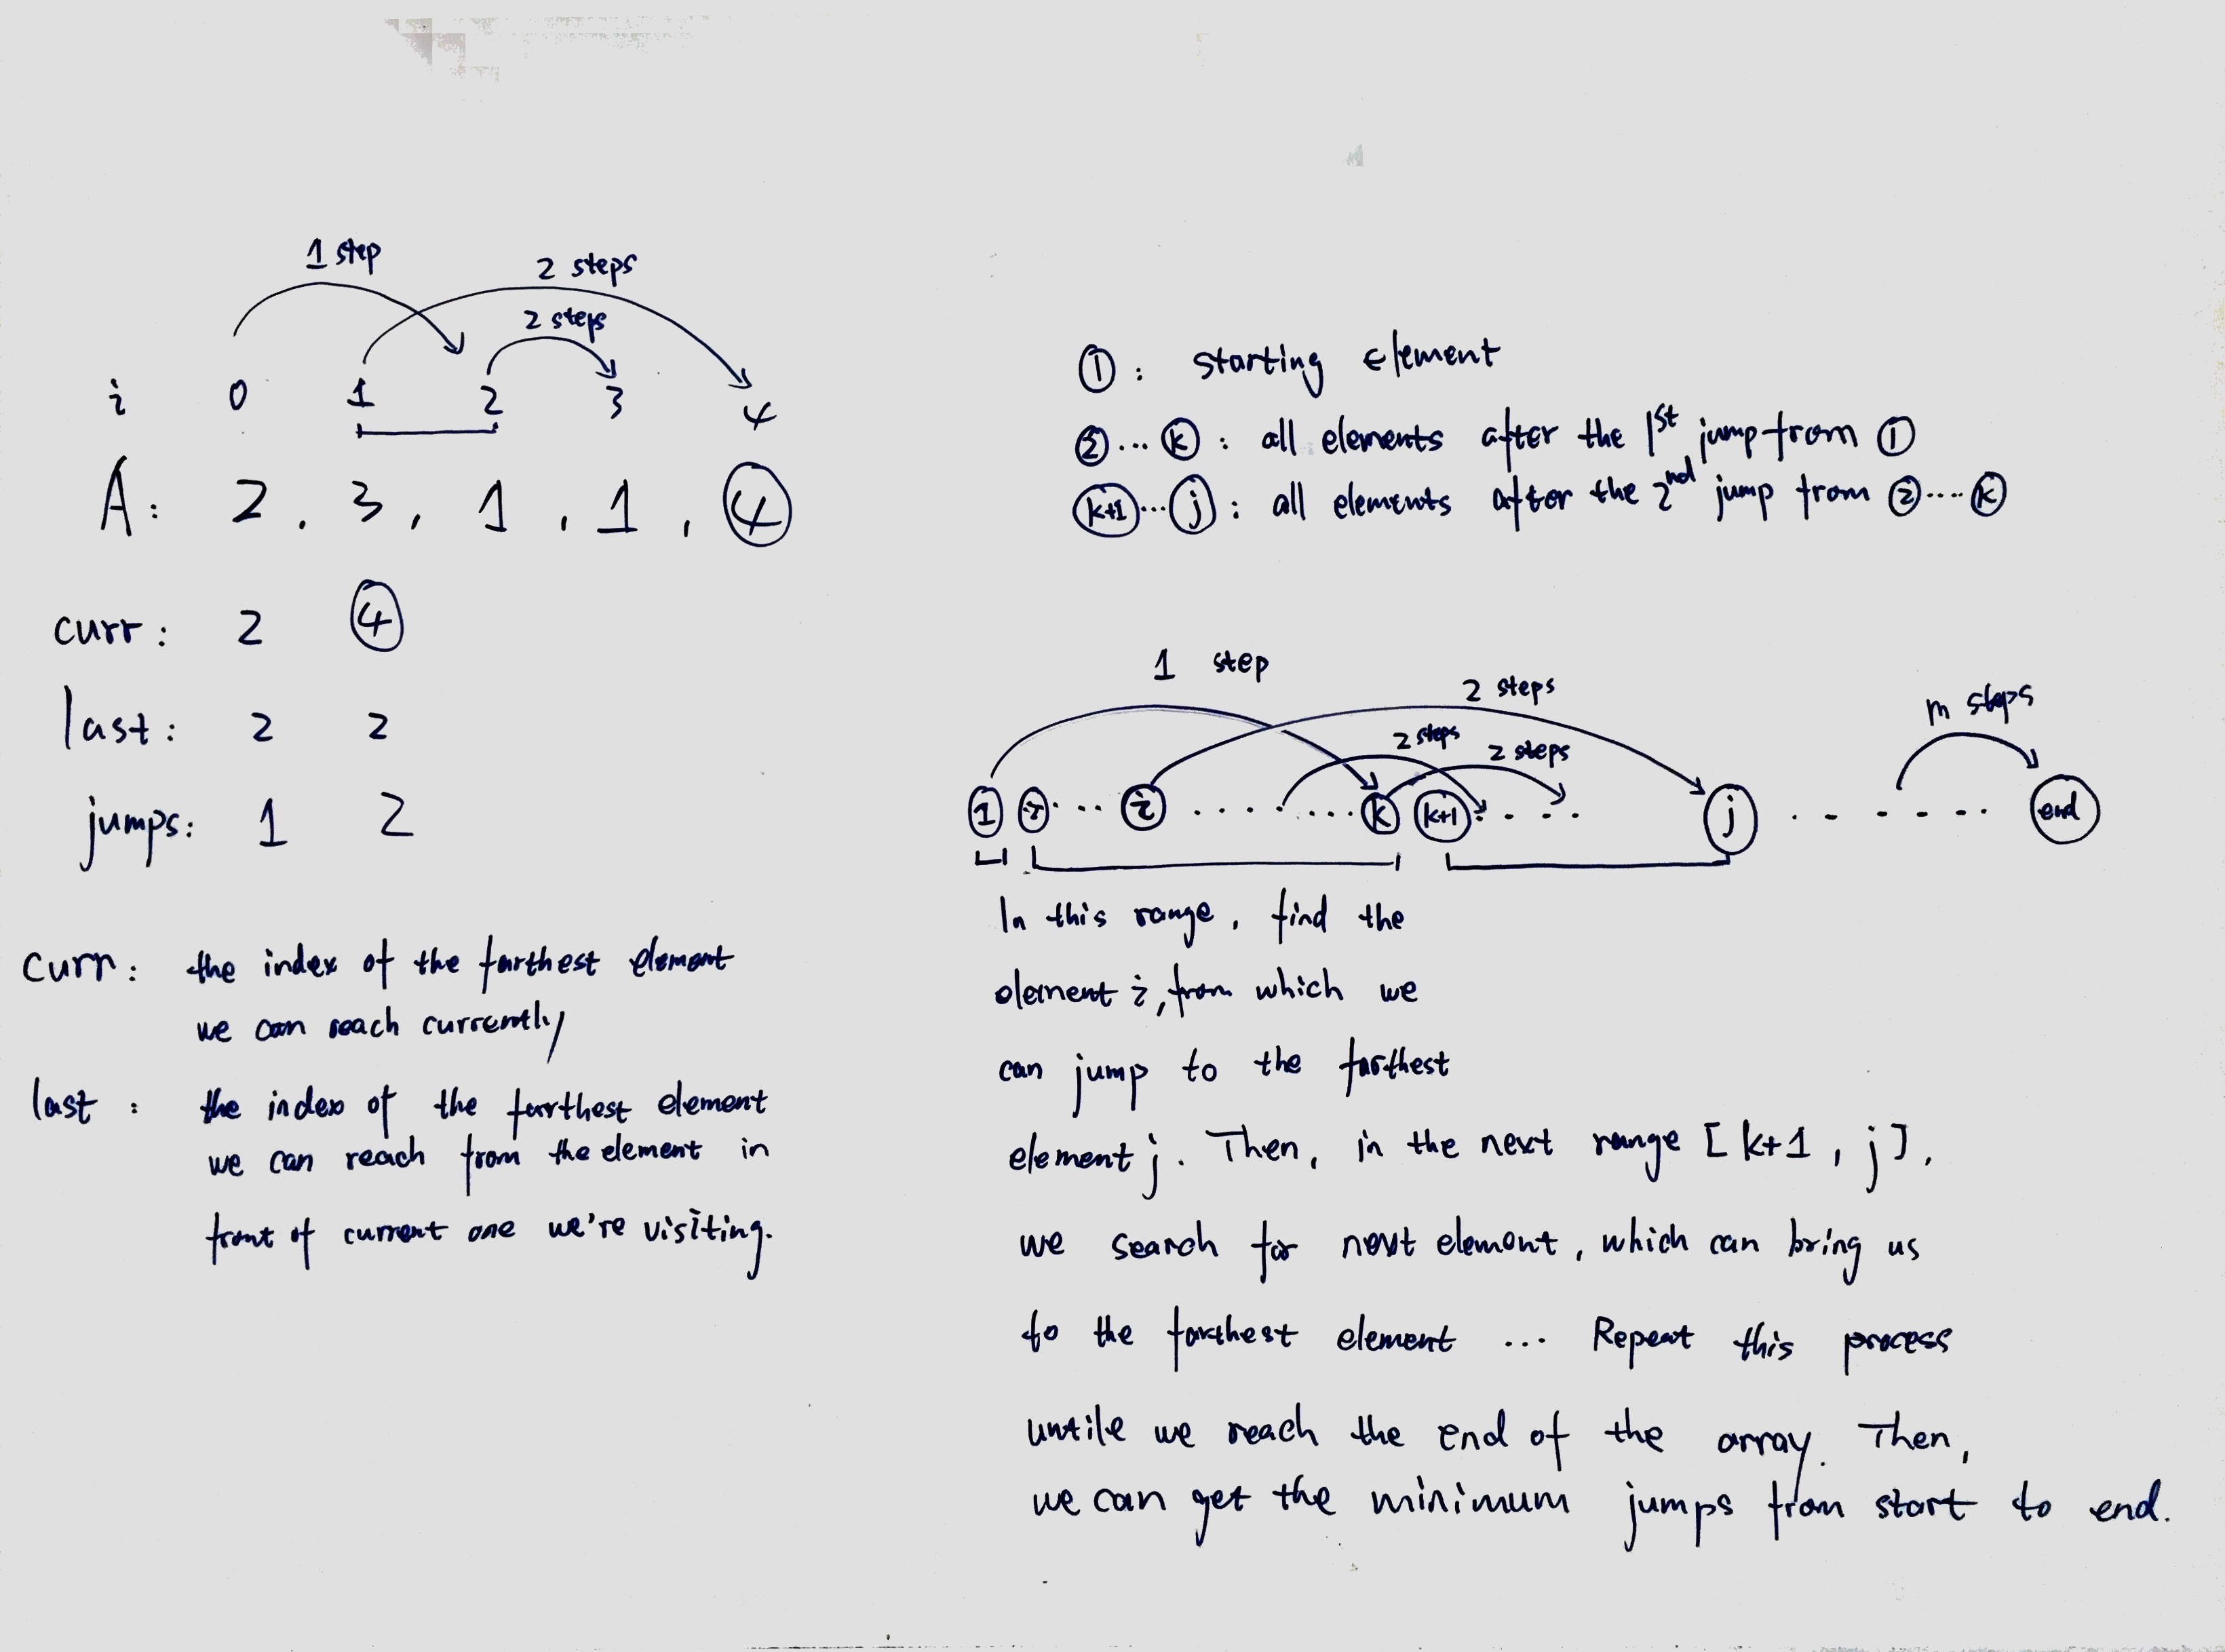
\includegraphics[width=\textwidth]{leetcode45.jpg}
    \centering \\
\end{figure}

\begin{lstlisting}[language=Python, caption=Problem45. Jump Game II]

class Solution(object):
    def jump(self, nums):
        n = len(nums)
        if n==0 or n==1: return 0
        jumps = lastCanReach = currCanReach = 0
        for i in xrange(n):
            if i==0:
                lastCanReach = nums[0]
                jumps = 1
            else:
                if i<=lastCanReach:
                    currCanReach = max(currCanReach, nums[i] + i)
                    if i==lastCanReach and currCanReach>lastCanReach:
                        lastCanReach = currCanReach
                        jumps += 1
            if lastCanReach>=n-1: break
        return jumps
\end{lstlisting}


\subsubsection{leetcode 122. Best Time to Buy and Sell Stock II}
Say you have an array for which the $i^{th}$ element is the price of a given stock on day $i$. Design an algorithm to find the maximum profit. You may complete as many transactions as you like (ie, buy one and sell one share of the stock multiple times). However, you may not engage in multiple transactions at the same time (ie, you must sell the stock before you buy again). \\

\begin{CJK*}{UTF8}{gbsn}
\noindent 解题思路:由于可以进行无限次的交易,那么只要是递增序列,就可以进行利润的累加。参考下面的示例图。
\end{CJK*}

\begin{figure}[h]
    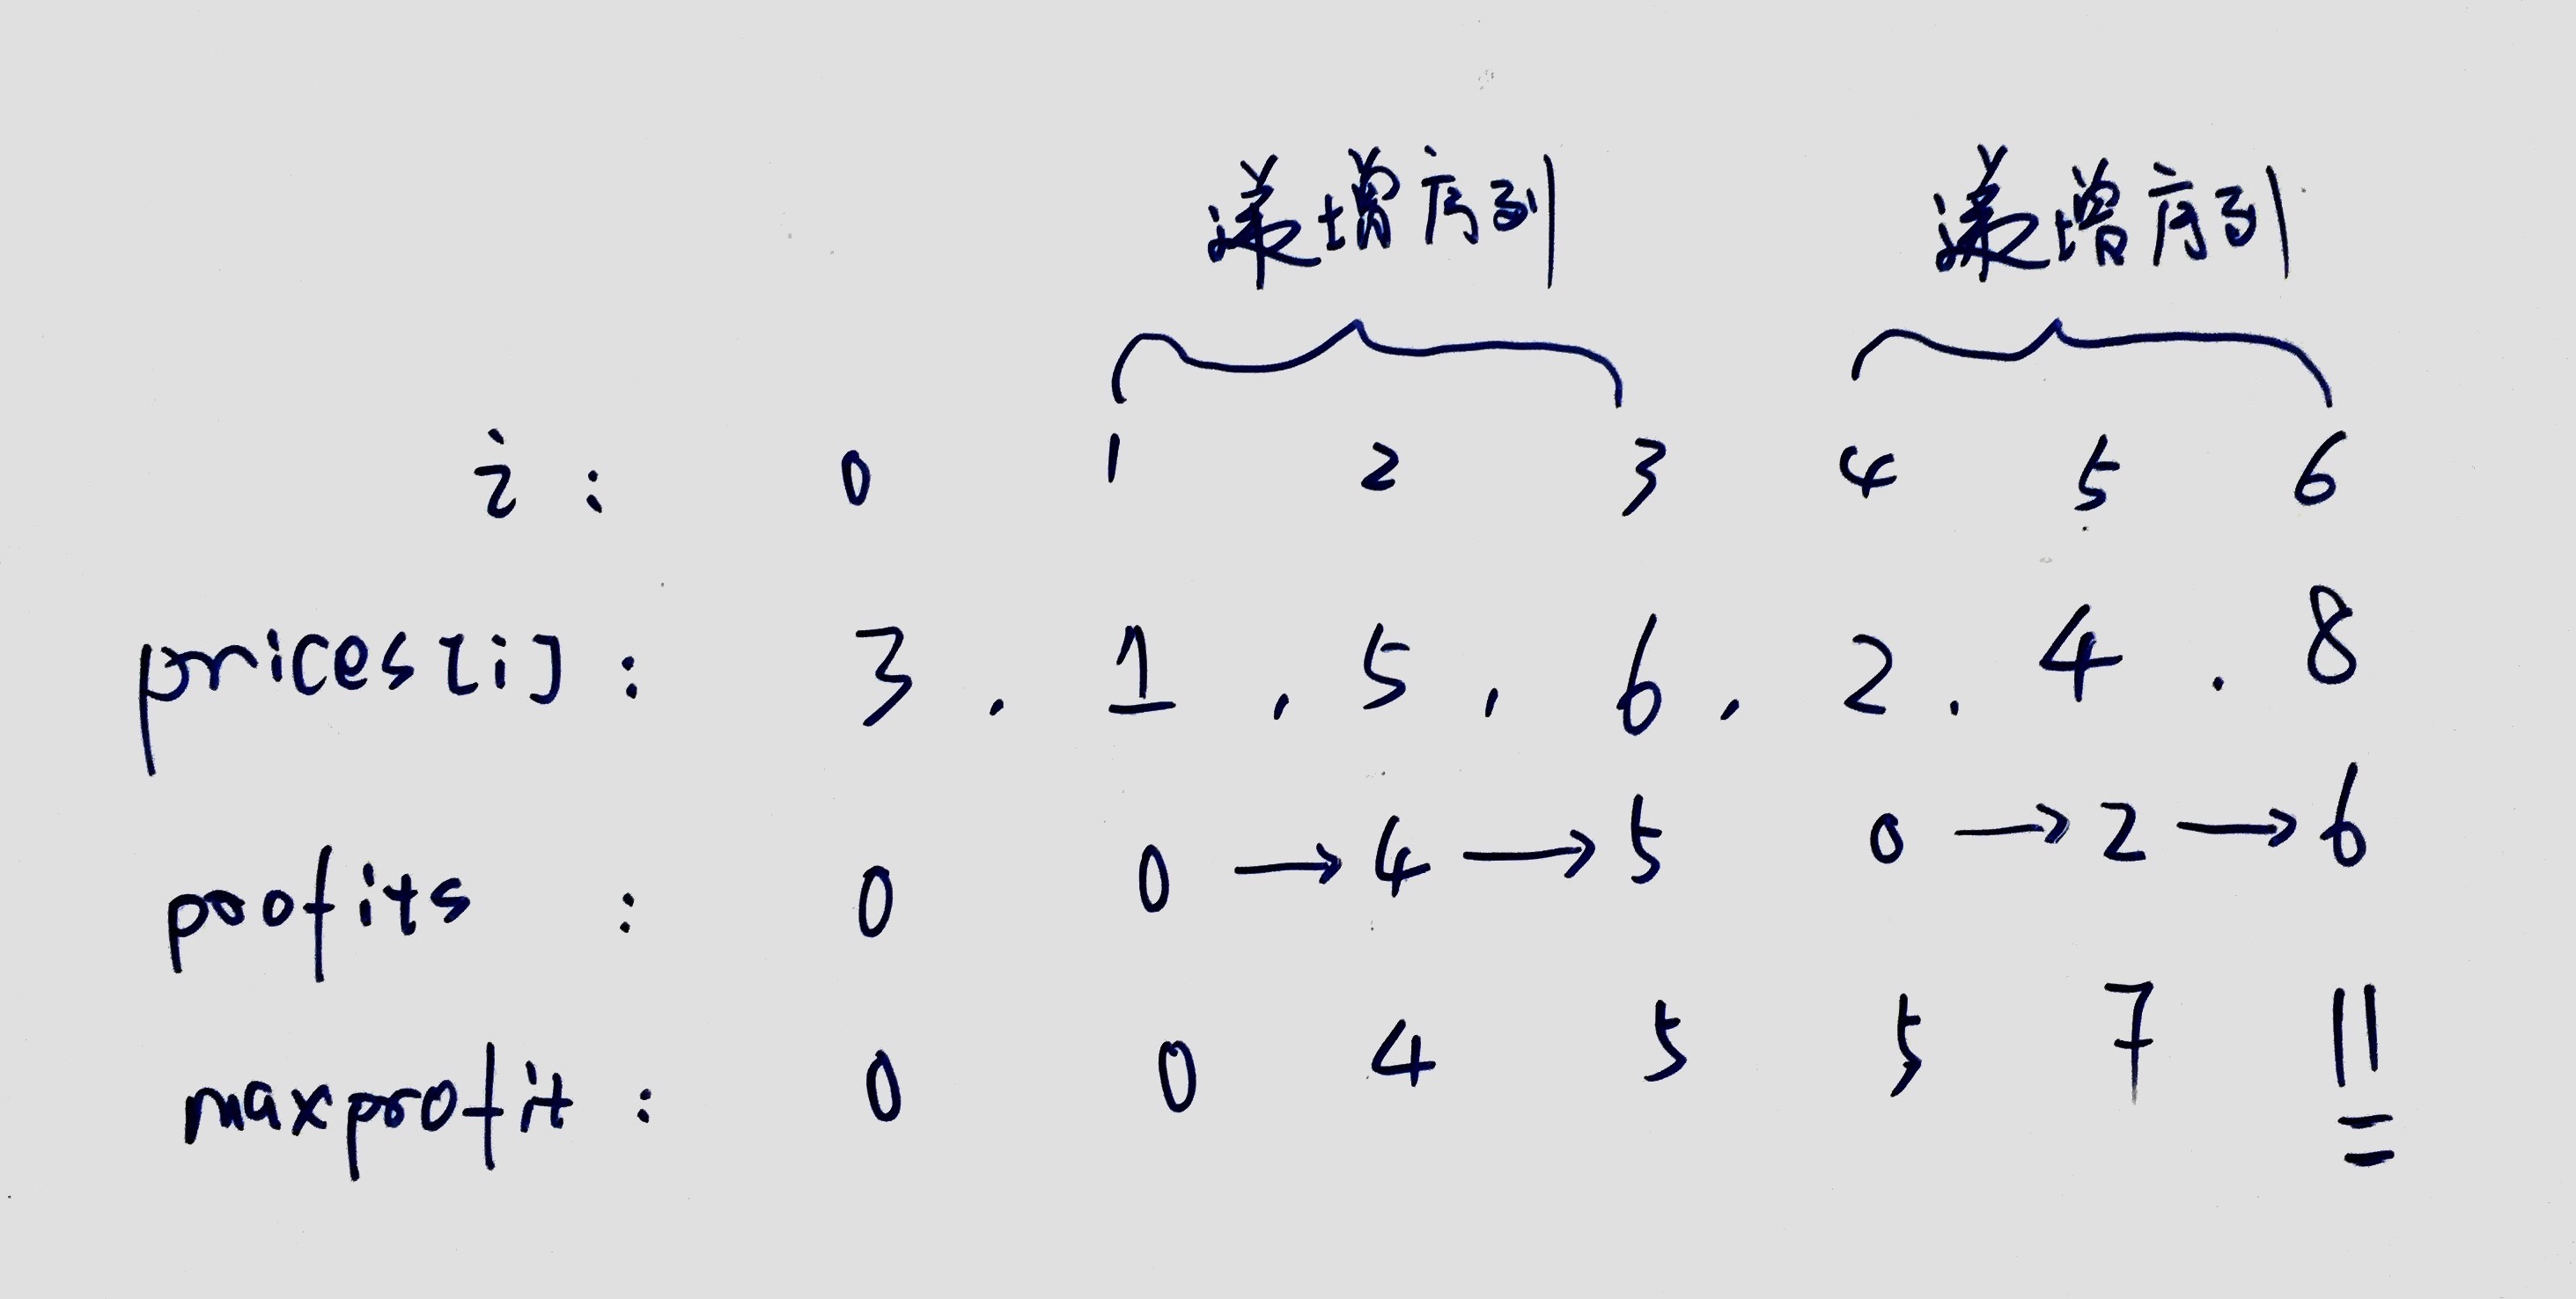
\includegraphics[width=\textwidth]{leetcode122.jpg}
    \centering \\
\end{figure}

\begin{lstlisting}[language=Python, caption=Problem122. Best Time to Buy and Sell Stock II]

class Solution(object):
    def maxProfit(self, prices):
        """
        :type prices: List[int]
        :rtype: int
        """
        maxprofits = 0
        n = len(prices)
        if n==0: return maxprofits
        for i in range(1,n):
            if prices[i] > prices[i-1]:
                maxprofits += prices[i] - prices[i-1]
        return maxprofits
\end{lstlisting}


\subsubsection{leetcode 216. Combination Sum III}
Find all possible combinations of $k$ numbers that add up to a number $n$, given that only numbers from 1 to 9 can be used and each combination should be a \textbf{unique} set of numbers. Ensure that numbers within the set are sorted in ascending order.

\noindent Examples:
\begin{enumerate}
    \item Input: k = 3, n = 7, Output: [[1,2,4]]
    \item Input: k = 3, n = 9, Output: [[1,2,6], [1,3,5], [2,3,4]]
\end{enumerate}

\begin{CJK*}{UTF8}{gbsn}
\noindent 解题思路:根据题目的描述,返回的结果中每个序列都是有序的,并且构成序列的数字都只出现一次。最直接的想法就是DFS遍历决策树,找出满足条件的所有子集。参考下面的示例图。
\end{CJK*}

\begin{figure}[h]
    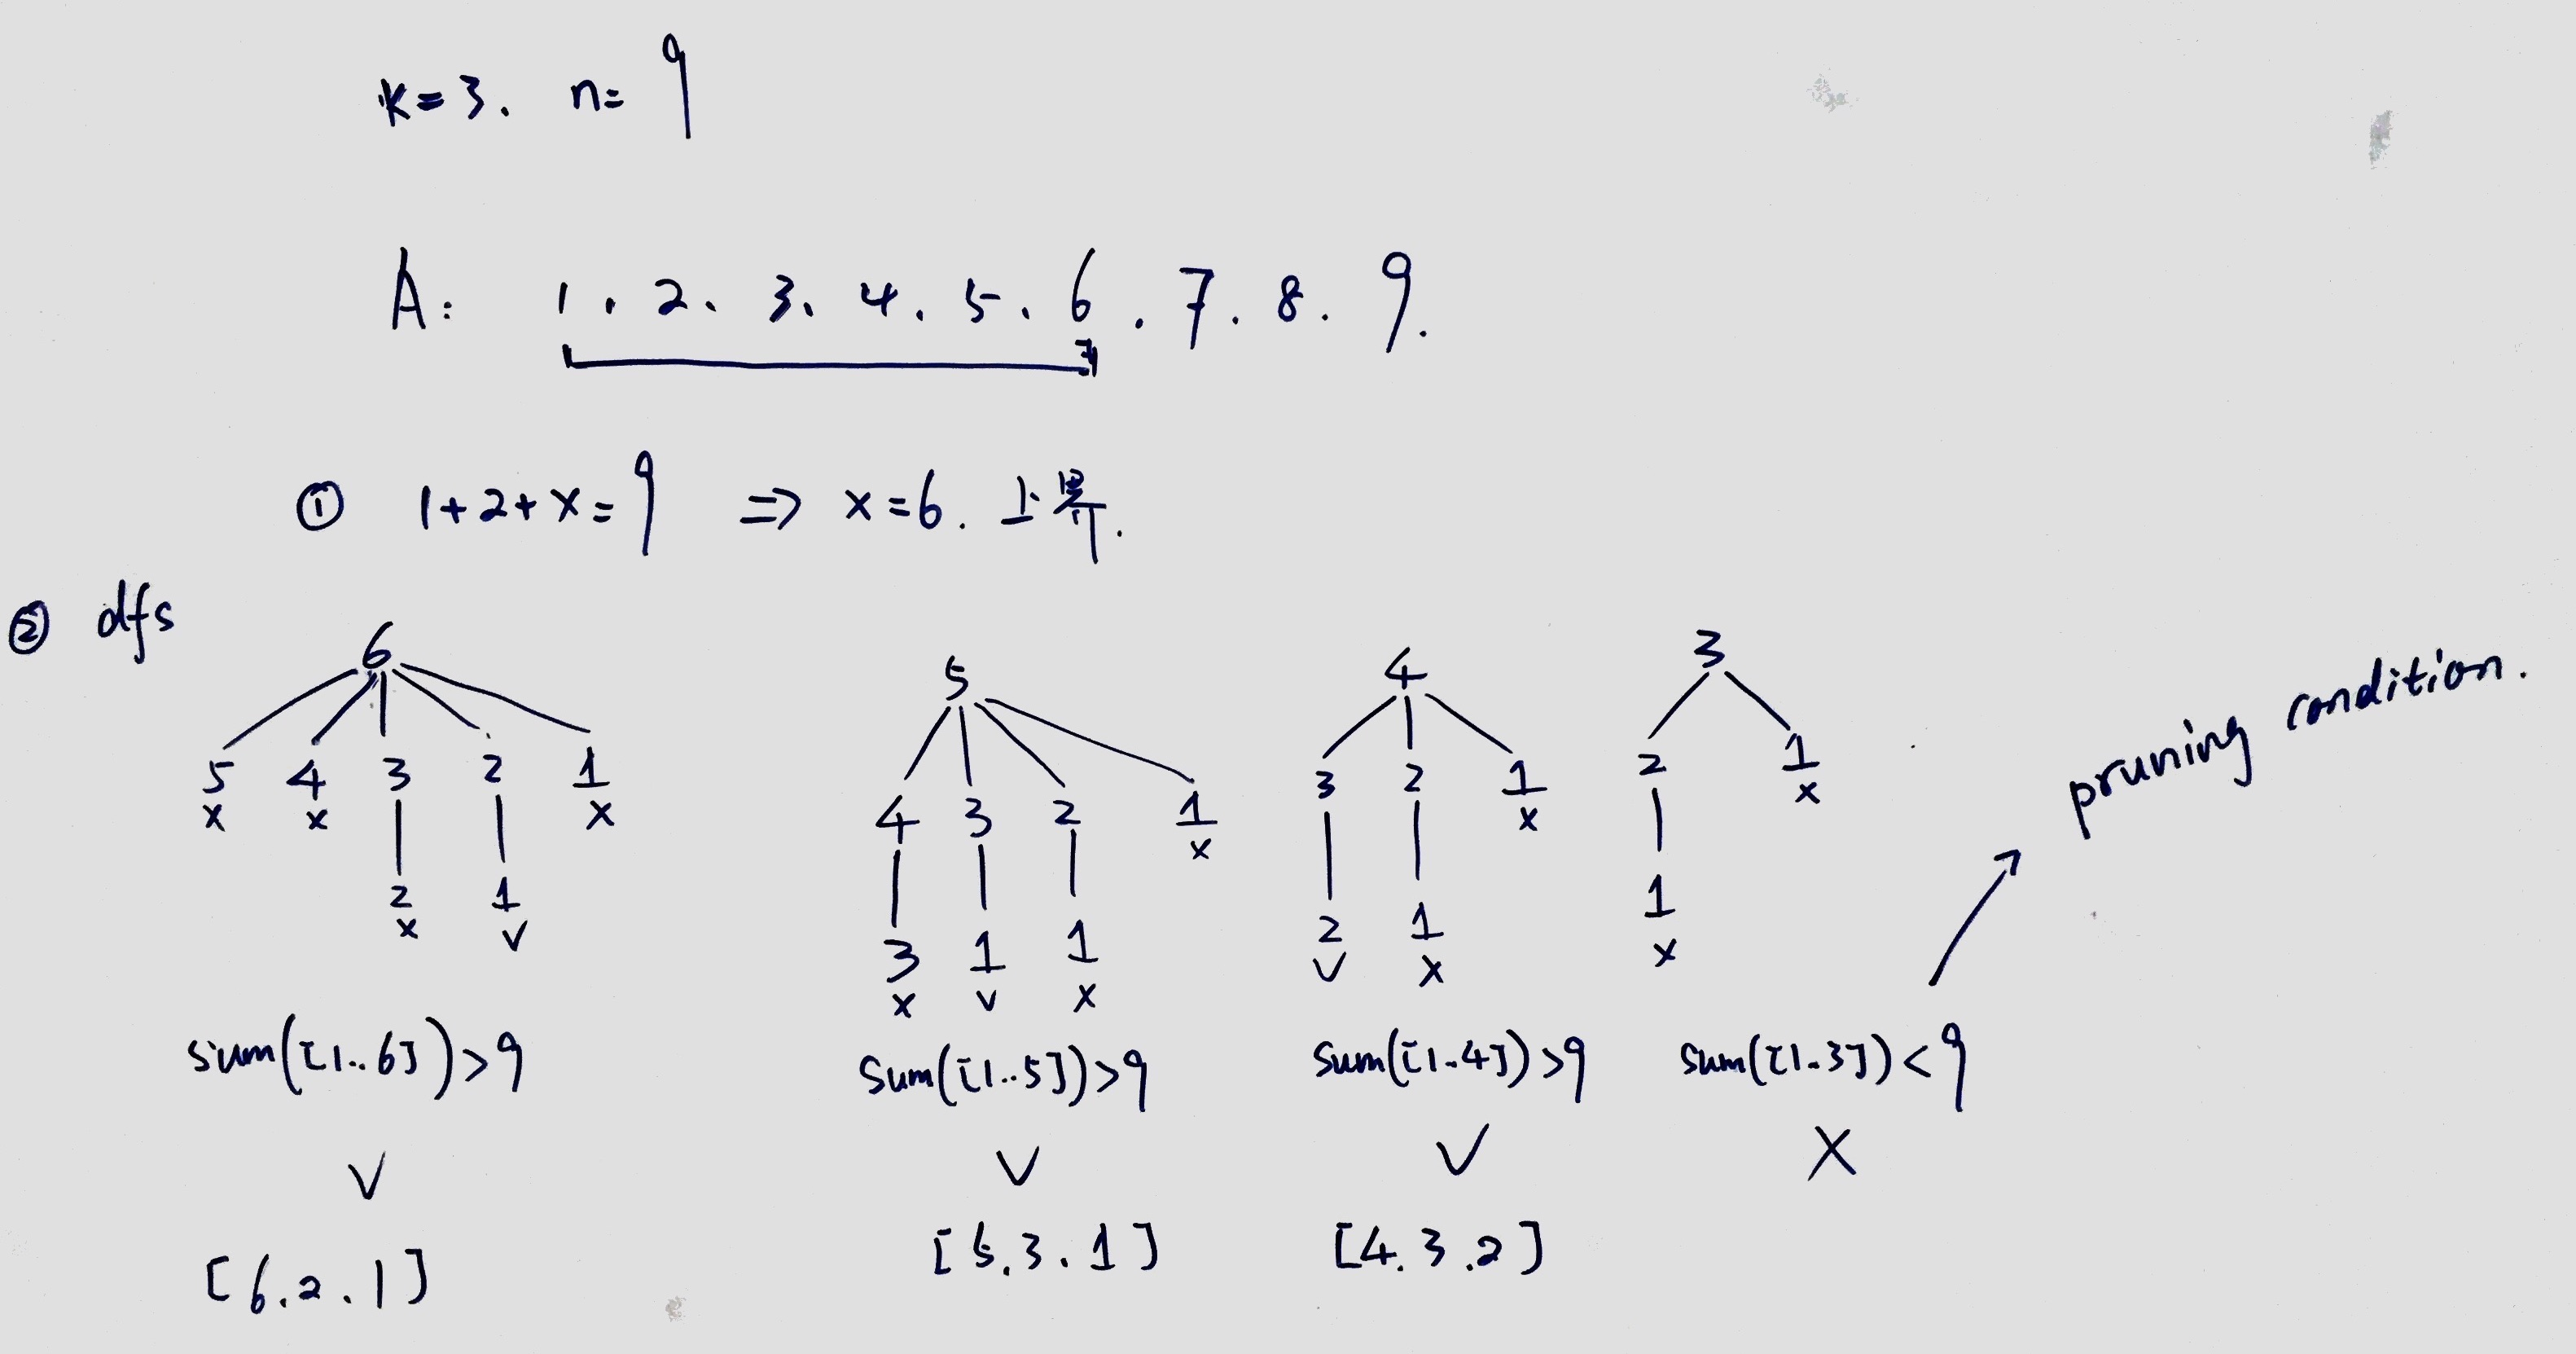
\includegraphics[width=\textwidth]{leetcode216.jpg}
    \centering \\
\end{figure}

\begin{lstlisting}[language=Python, caption=Problem216. Combination Sum III]

class Solution(object):
    def combinationSum3(self, k, n):
        """
        :type k: int
        :type n: int
        :rtype: List[List[int]]
        """
        def dfs(nums, start, k, n, valuelist):
            if n==0 and k==0: res.append(valuelist)
            if k==0: return
            for x in xrange(start, len(nums)):
                if n < nums[x]: return
                dfs(nums, x+1, k-1, n-nums[x], valuelist+[nums[x]])
        
        res = []
        nums = [i for i in range(1,10)]
        dfs(nums, 0, k, n, [])
        return res
\end{lstlisting}


\subsubsection{leetcode 11. Container With Most Water}
Given $n$ non-negative integers $a_1, a_2, \dots, a_n$, where each represents a point at coordinate $(i, a_i)$. $n$ vertical lines are drawn such that the two endpoints of line $i$ is at $(i, a_i)$ and $(i, 0)$. Find two lines, which together with x-axis forms a container, such that the container contains the most water. Note: You may not slant the container. \\

\begin{CJK*}{UTF8}{gbsn}
\noindent 解题思路:这道题与leetcode42 Trapping Rain Water的解题思路类似,区别在于leetcode42每次的计算是由三个因素(左侧,自己,右侧的高度)决定,而本题是由两个因素(左侧和右侧两个隔板)决定的。两个隔板的矮的那一个的高度乘以两个隔板的间距就是储水量。
\end{CJK*}

\begin{figure}[h]
    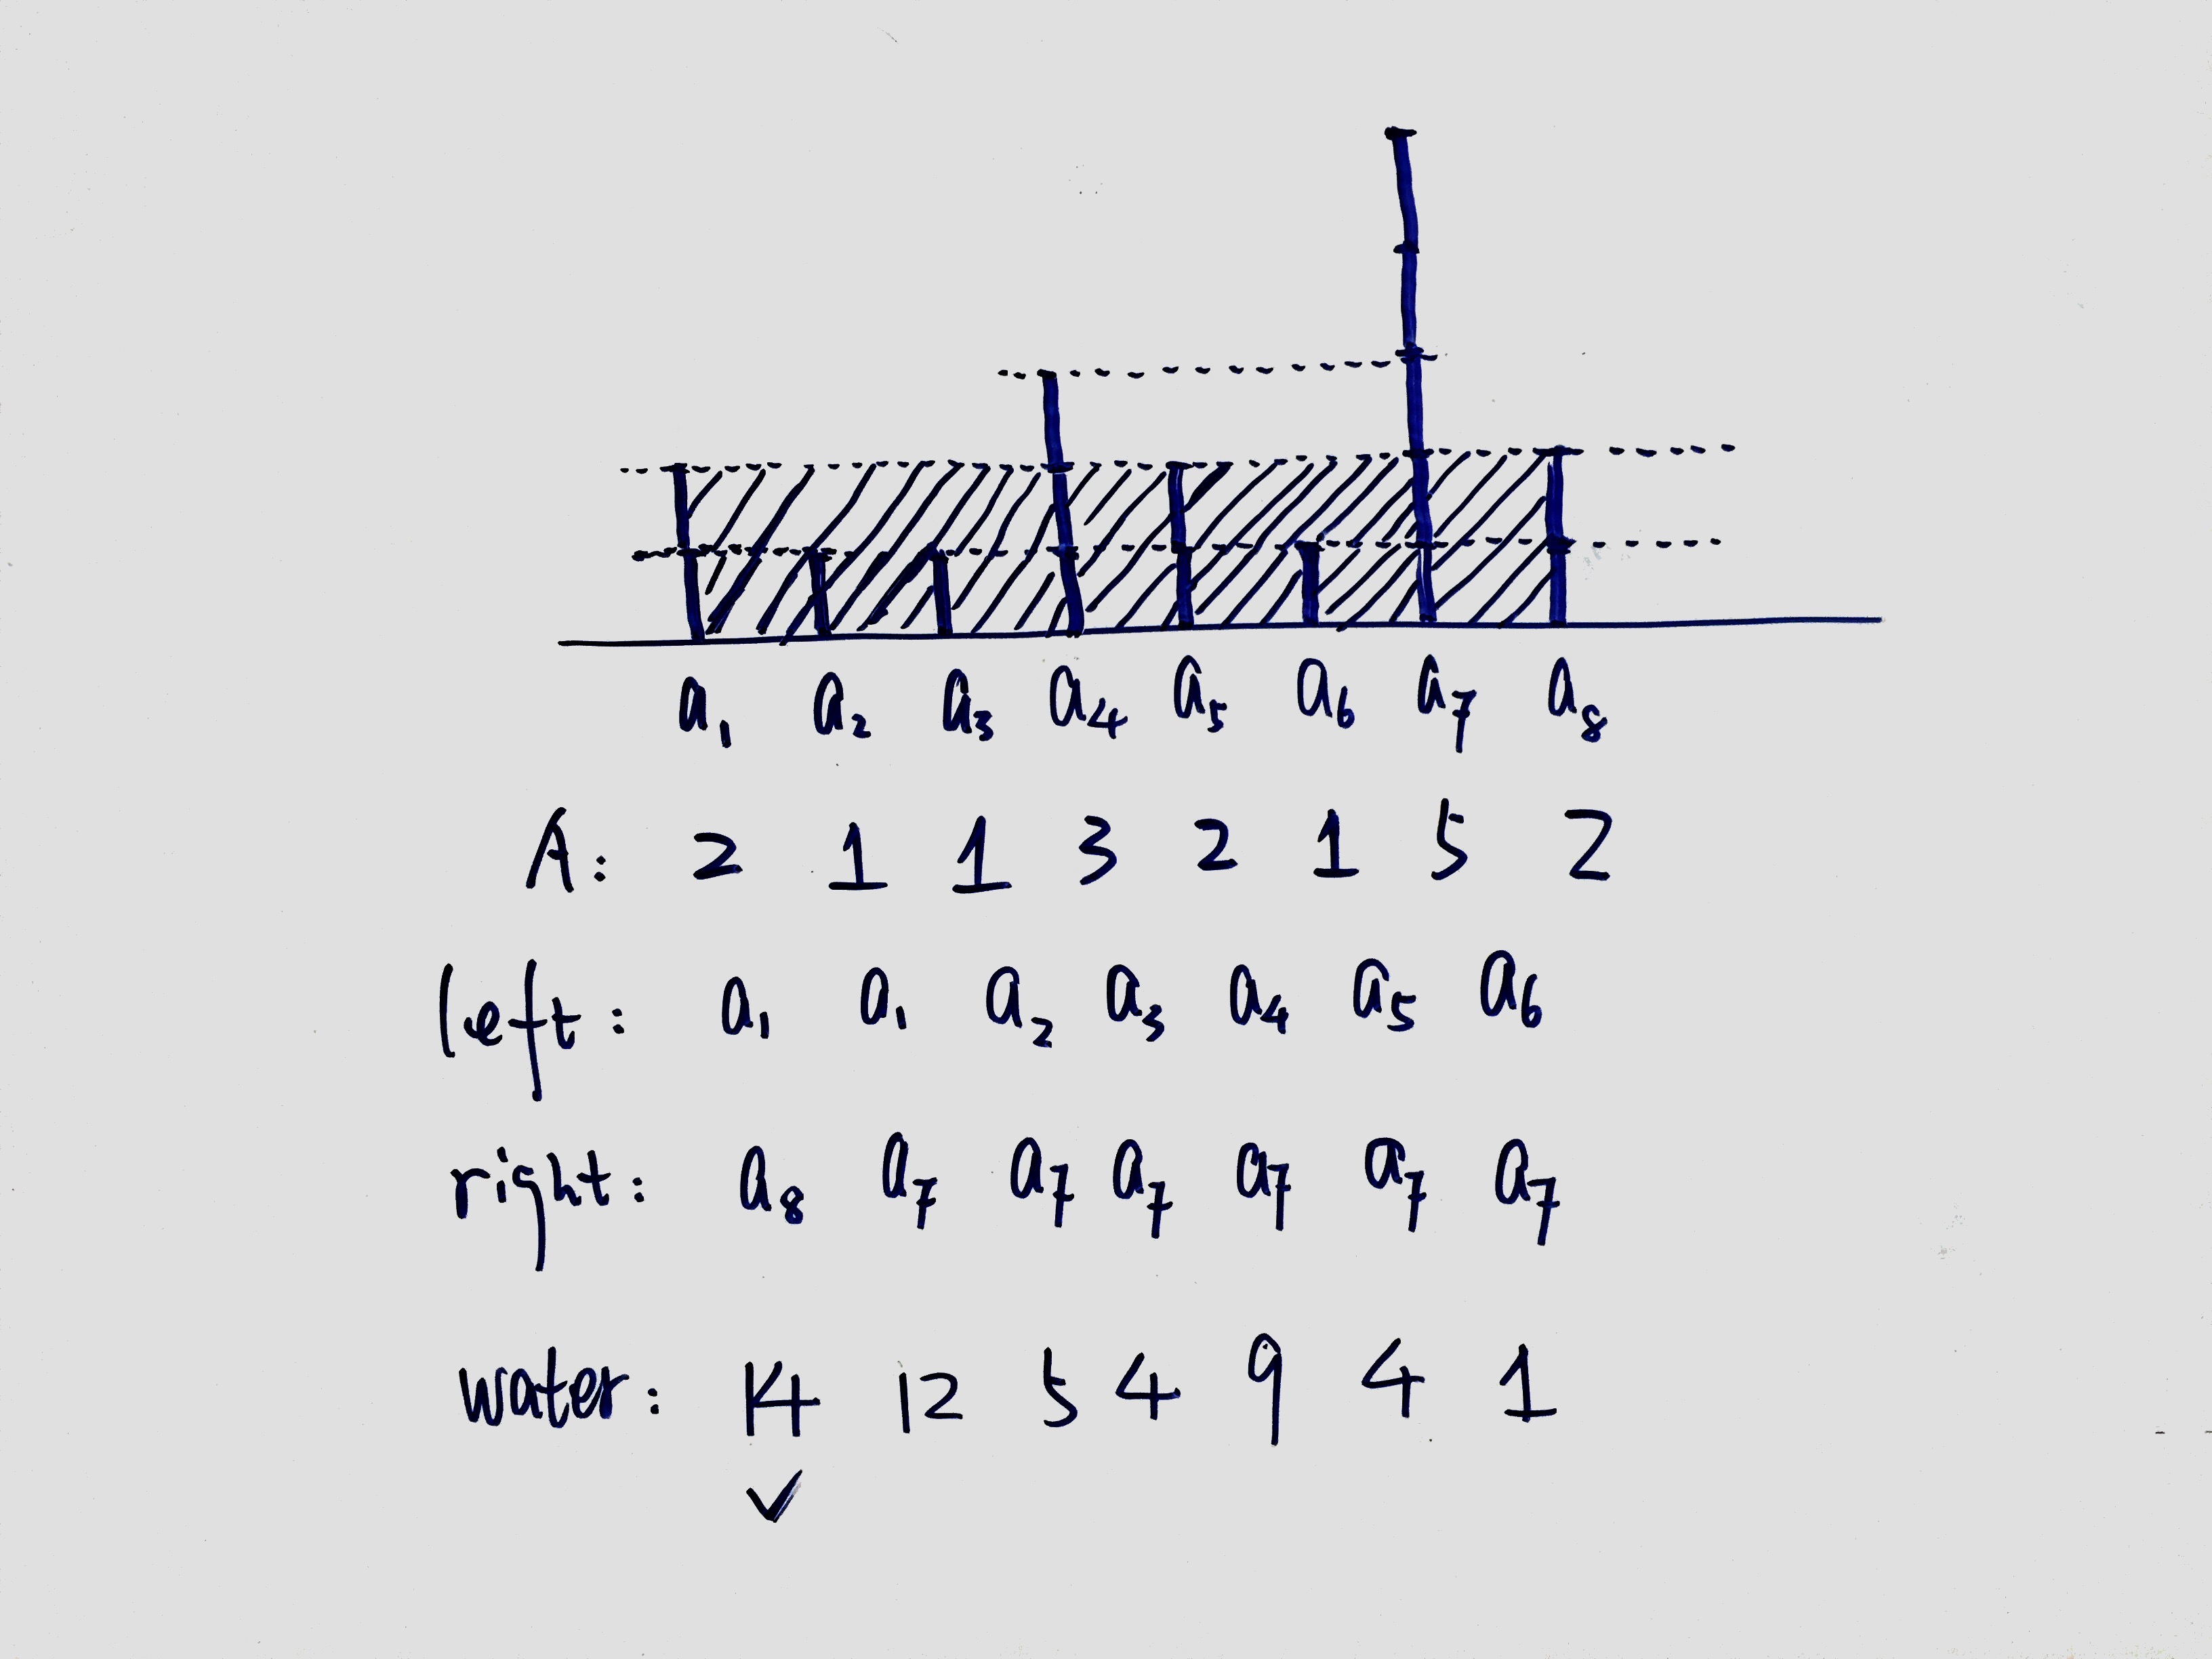
\includegraphics[width=\textwidth]{leetcode11.jpg}
    \centering \\
\end{figure}

\begin{lstlisting}[language=Python, caption=Problem11. Container With Most Water]

class Solution(object):
    def maxArea(self, height): # RT: O(n)
        """
        :type height: List[int]
        :rtype: int
        """
        n = len(height)
        left, right = 0, n-1
        maxarea = 0
        while left < right:
            area = min(height[left], height[right]) * abs(right-left)
            maxarea = max(maxarea, area)
            if height[left] < height[right]:
                left += 1
            else:
                right -= 1
        return maxarea
\end{lstlisting}



\subsubsection{leetcode 153. Find Minimum in Rotated Sorted Array}
Suppose a \textbf{sorted} array is \textbf{rotated} at some pivot unknown to you beforehand. (i.e., 0 1 2 4 5 6 7 might become 4 5 6 7 0 1 2). Find the minimum element. You may assume \textbf{no duplicate} exists in the array. \\

\begin{CJK*}{UTF8}{gbsn}
\noindent 解题思路:这道题与leetcode 33 Search in Rotated Sorted Array的解题思路类似,只是在移动start和end的判断条件上有所区别。两题都是考查binary search算法。参见下面示例图。
\end{CJK*}

\begin{figure}[h]
    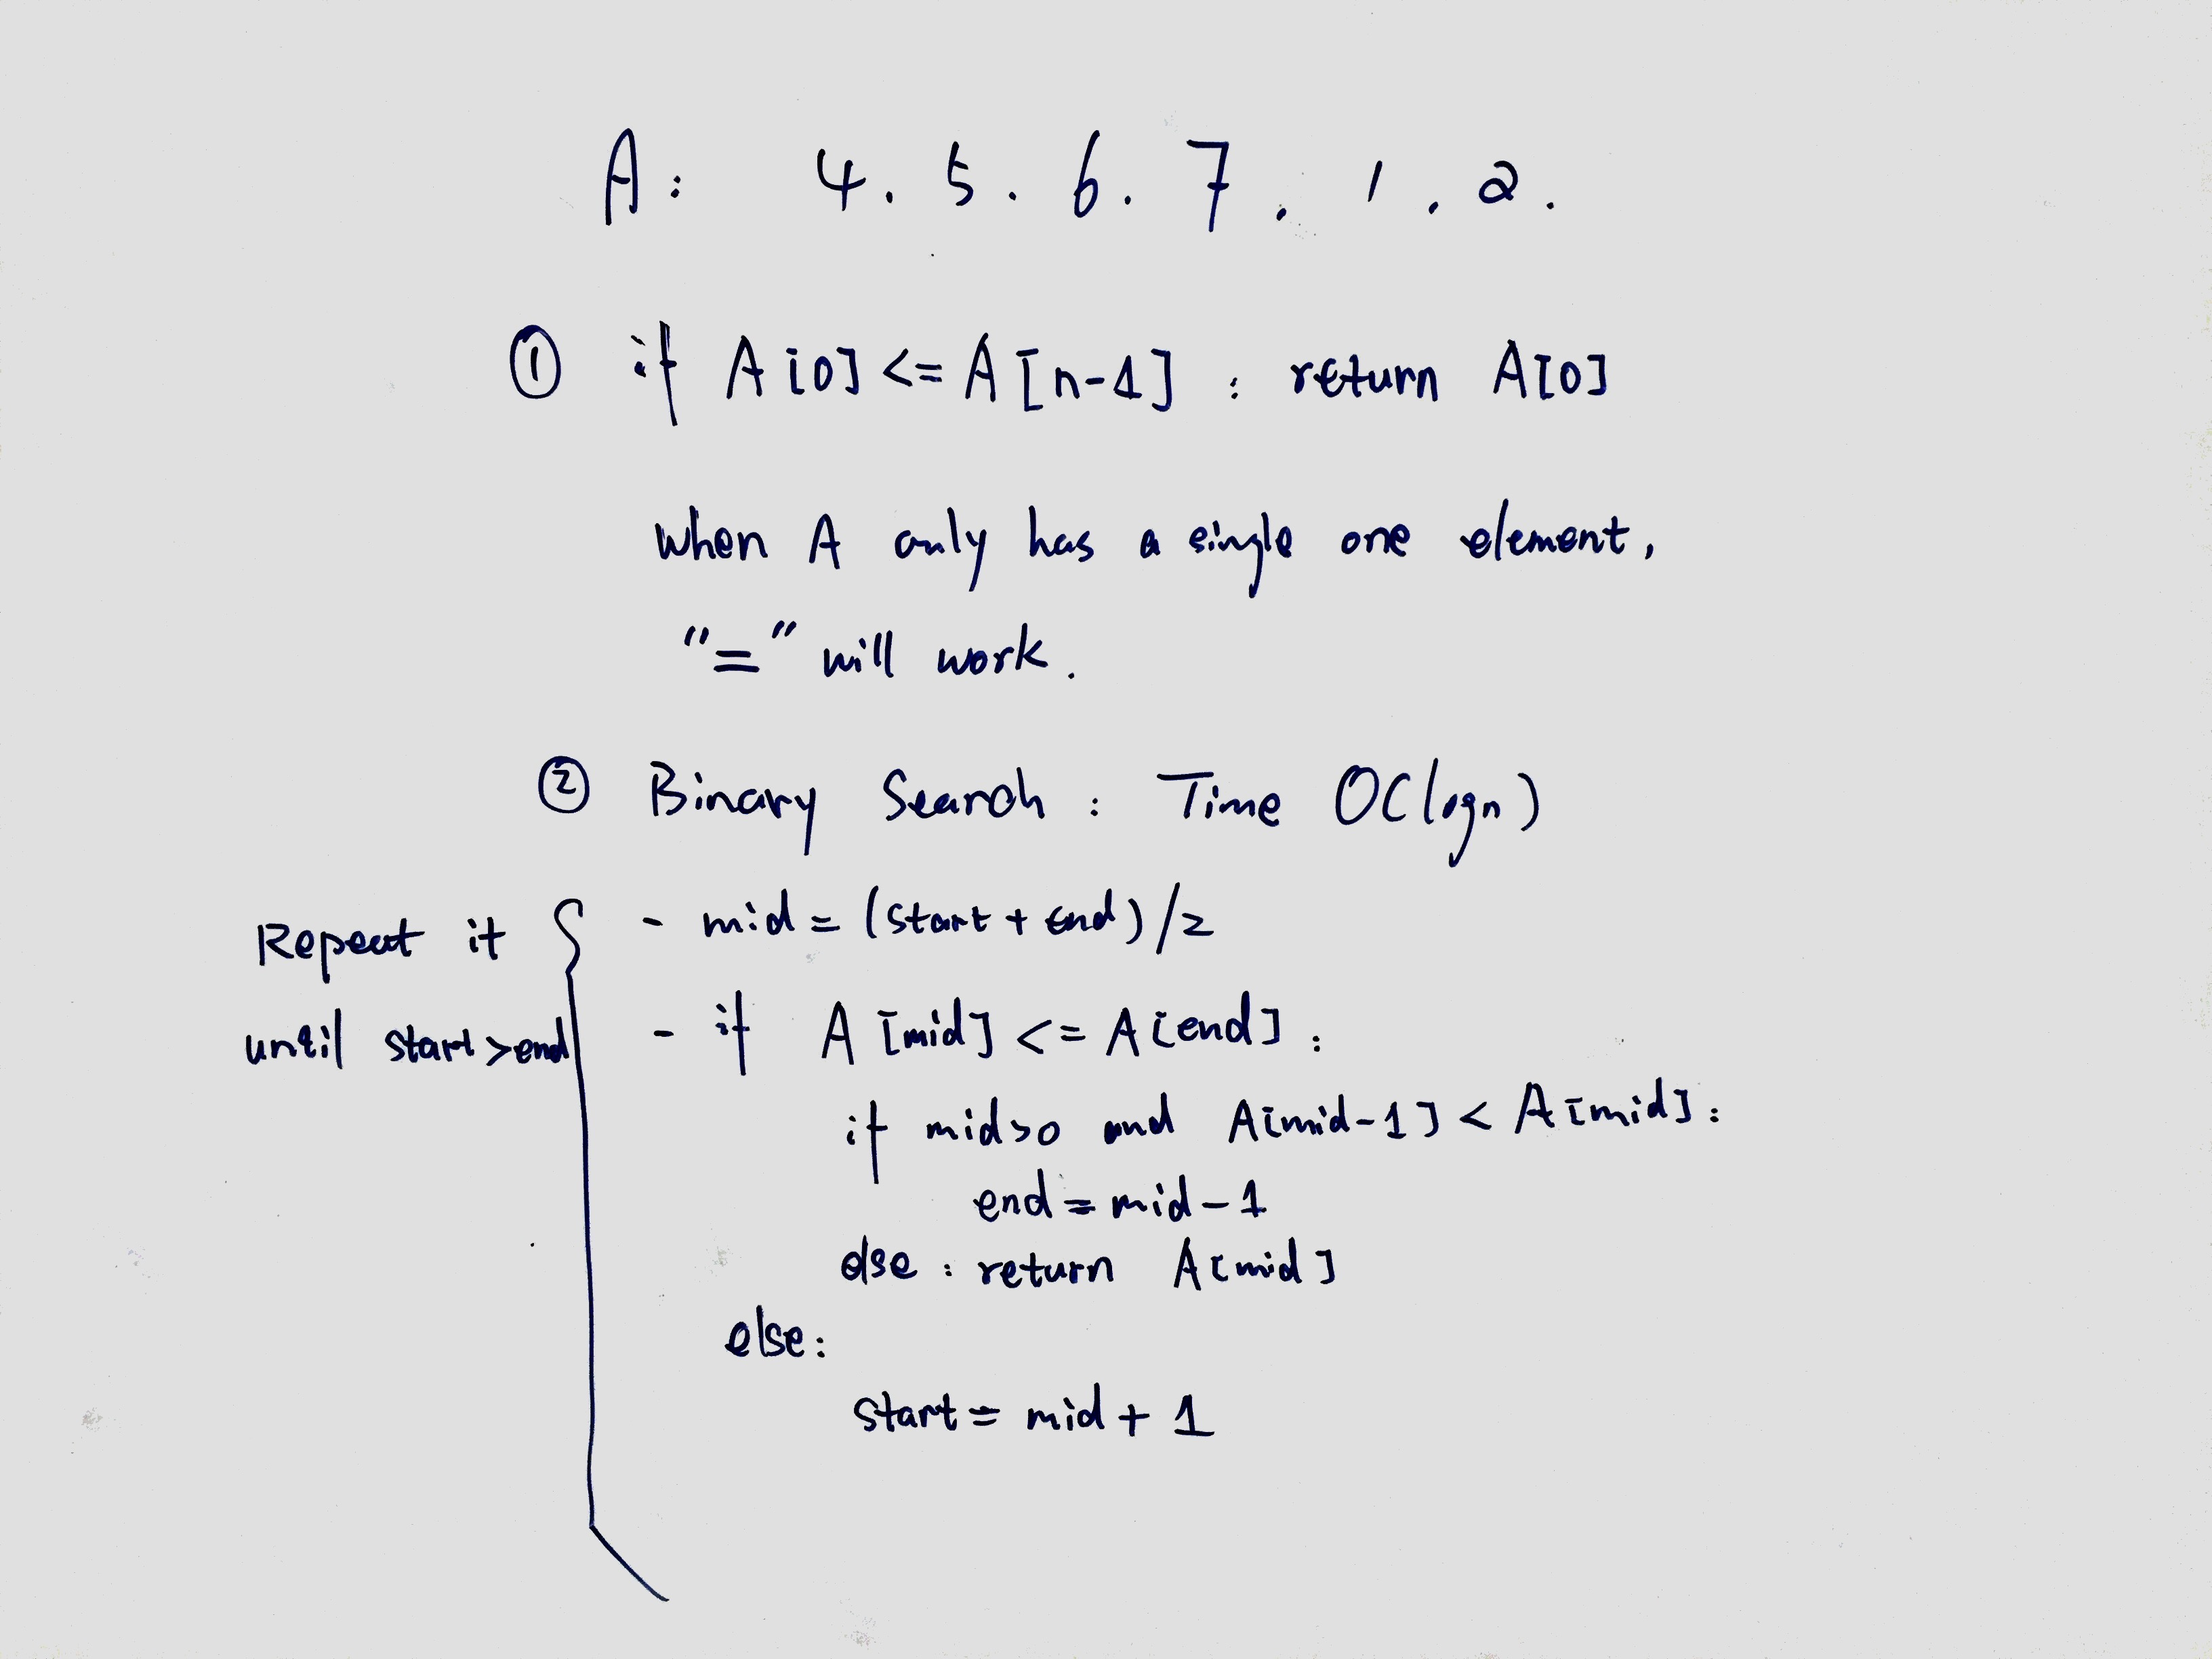
\includegraphics[width=\textwidth]{leetcode153.jpg}
    \centering \\
\end{figure}

\begin{lstlisting}[language=Python, caption=Problem153. Find Minimum in Rotated Sorted Array]

class Solution(object):
    def findMin(self, nums): # RT: O(logn)
        n = len(nums)
        if nums[0]<=nums[-1]:
            return nums[0]
        start, end = 0, n-1
        while start <= end:
            mid = (start+end)/2
            if nums[mid] <= nums[end]:
                if mid > 0 and nums[mid-1]<=nums[mid]:
                    end = mid-1
                else:
                    return nums[mid]
            else:
                start = mid+1
        return -1
\end{lstlisting}


\subsubsection{leetcode 154. Find Minimum in Rotated Sorted Array II}
Follow up for "Find Minimum in Rotated Sorted Array": What if duplicates are allowed? Would this affect the run-time complexity? How and why? \\

\noindent Suppose a sorted array is rotated at some pivot unknown to you beforehand. (i.e., 0 1 2 4 5 6 7 might become 4 5 6 7 0 1 2). Find the minimum element. You may assume no duplicate exists in the array. \\

\begin{CJK*}{UTF8}{gbsn}
\noindent 解题思路:这道题与leetcode 81. Search in Rotated Sorted Array II的解题思路类似,只是在移动start和end的判断条件上有所区别。两题都是考查存在重复元素的时候,binary search算法的应用,以及对binary search算法性能的评估。这道题在面试的时候应该是考查对BS搜索算法最差时间复杂度情况的讨论。
\end{CJK*}

\begin{lstlisting}[language=Python, caption=Problem154. Find Minimum in Rotated Sorted Array II]

class Solution(object):
    # binary search + recursion
    def findMin(self, nums): # RT: O(logn), the worse case in O(n) time
        n = len(nums)
        minval = nums[0]
        if n==1 or nums[0]<nums[-1]:
            return minval
        start, end = 0, n-1
        while start <= end:
            mid = (start+end)/2
            minval = min(minval, nums[mid])
            if nums[mid] < nums[end]:
                end = mid-1
            elif nums[mid] > nums[end]:
                start = mid+1
            else:
                if start < mid:
                    minval = min(minval, self.findMin(nums[start:mid+1]))
                if mid+1 < end:
                    minval = min(minval, self.findMin(nums[mid+1:end+1]))
                break
        return minval
\end{lstlisting}


\subsubsection{leetcode 57. Insert Interval}
Given a set of non-overlapping intervals, insert a new interval into the intervals (merge if necessary). You may assume that the intervals were initially \textbf{sorted} according to their start times. \\

\noindent Example 1: Given intervals [1,3],[6,9], insert and merge [2,5] in as [1,5],[6,9]. \\

\noindent Example 2: Given [1,2],[3,5],[6,7],[8,10],[12,16], insert and merge [4,9] in as [1,2],[3,10],[12,16]. This is because the new interval [4,9] overlaps with [3,5],[6,7],[8,10]. \\

\begin{lstlisting}[language=Python, caption=Problem57. Insert Interval]

# Definition for an interval.
# class Interval(object):
#     def __init__(self, s=0, e=0):
#         self.start = s
#         self.end = e

class Solution(object):
    def insert(self, intervals, newInterval):  # RT: O(n)
        """
        :type intervals: List[Interval]
        :type newInterval: Interval
        :rtype: List[Interval]
        """
        res = []
        n = len(intervals)
        if n==0: 
            res.append(newInterval) 
            return res
        i = 0
        while i < n:
            if intervals[i].end < newInterval.start:
                res.append(intervals[i])
                i += 1
            else:
                break
        if i==n:
            res.append(newInterval)
        
        while i < n:
            newInterval.start = min(newInterval.start, intervals[i].start)
            if intervals[i].start <= newInterval.end:
                newInterval.end = max(newInterval.end, intervals[i].end)
                if i==n-1:
                    res.append(newInterval)
            if intervals[i].start > newInterval.end:
                res.append(newInterval)
                break
            i += 1
        
        while i < n: 
            res.append(intervals[i])
            i += 1
            
        return res
\end{lstlisting}



\subsubsection{leetcode 287. Find the Duplicate Number}
Given an array nums containing $n+1$ integers where each integer is between 1 and n (inclusive), prove that at least one duplicate number must exist. Assume that there is only one duplicate number, find the duplicate one. \\

\noindent Note:
\begin{enumerate}
    \item You must not modify the array (assume the array is read only).
    \item You must use only constant, O(1) extra space.
    \item Your runtime complexity should be less than O($n^2$).
    \item There is only one duplicate number in the array, but it could be repeated more than once.
\end{enumerate}

\begin{CJK*}{UTF8}{gbsn}
\noindent 解题思路:这道题比较难,需要对问题重新建模。参见下面示例图。因为题目限定了长为$n$的数组中填充的数值范围在$1 \dots n$,所以数组中的数值和数组的索引值都在这个范围内。假设A[i]=j,那么我们可以构建一个有向图,图中结点的结构可以用一个元组$(i,A[i])$表示;如果图中有两个结点$(i,A[i])$和$(j,A[j])$,当且仅当$A[i]==j$时,存在一条从结点$(i,A[i])$到结点$(j,A[j])$的有向边。如示例图所示,在构建这个有向图的过程中,我们可以观察到,如果数组中存在重复数值,那么在图中一定出现一个环,并且数组中构成环路以后其余数值将构成另外一个有向无环图DAG。为了找到重复数值,只需关注这个有环的图。我们再来看分析一下这个有环图,从起点开始到构成环所经过的路径构成了$\rho$形,这就与leetcode 141/142 Linked List Cycle I/II两题相似:首先用一次遍历确定是否有环;如果环存在,再遍历一遍确定环的起始位置,即重复元素。这部分的算法设计与leetcode142一致。
\end{CJK*}

\begin{figure}[h]
    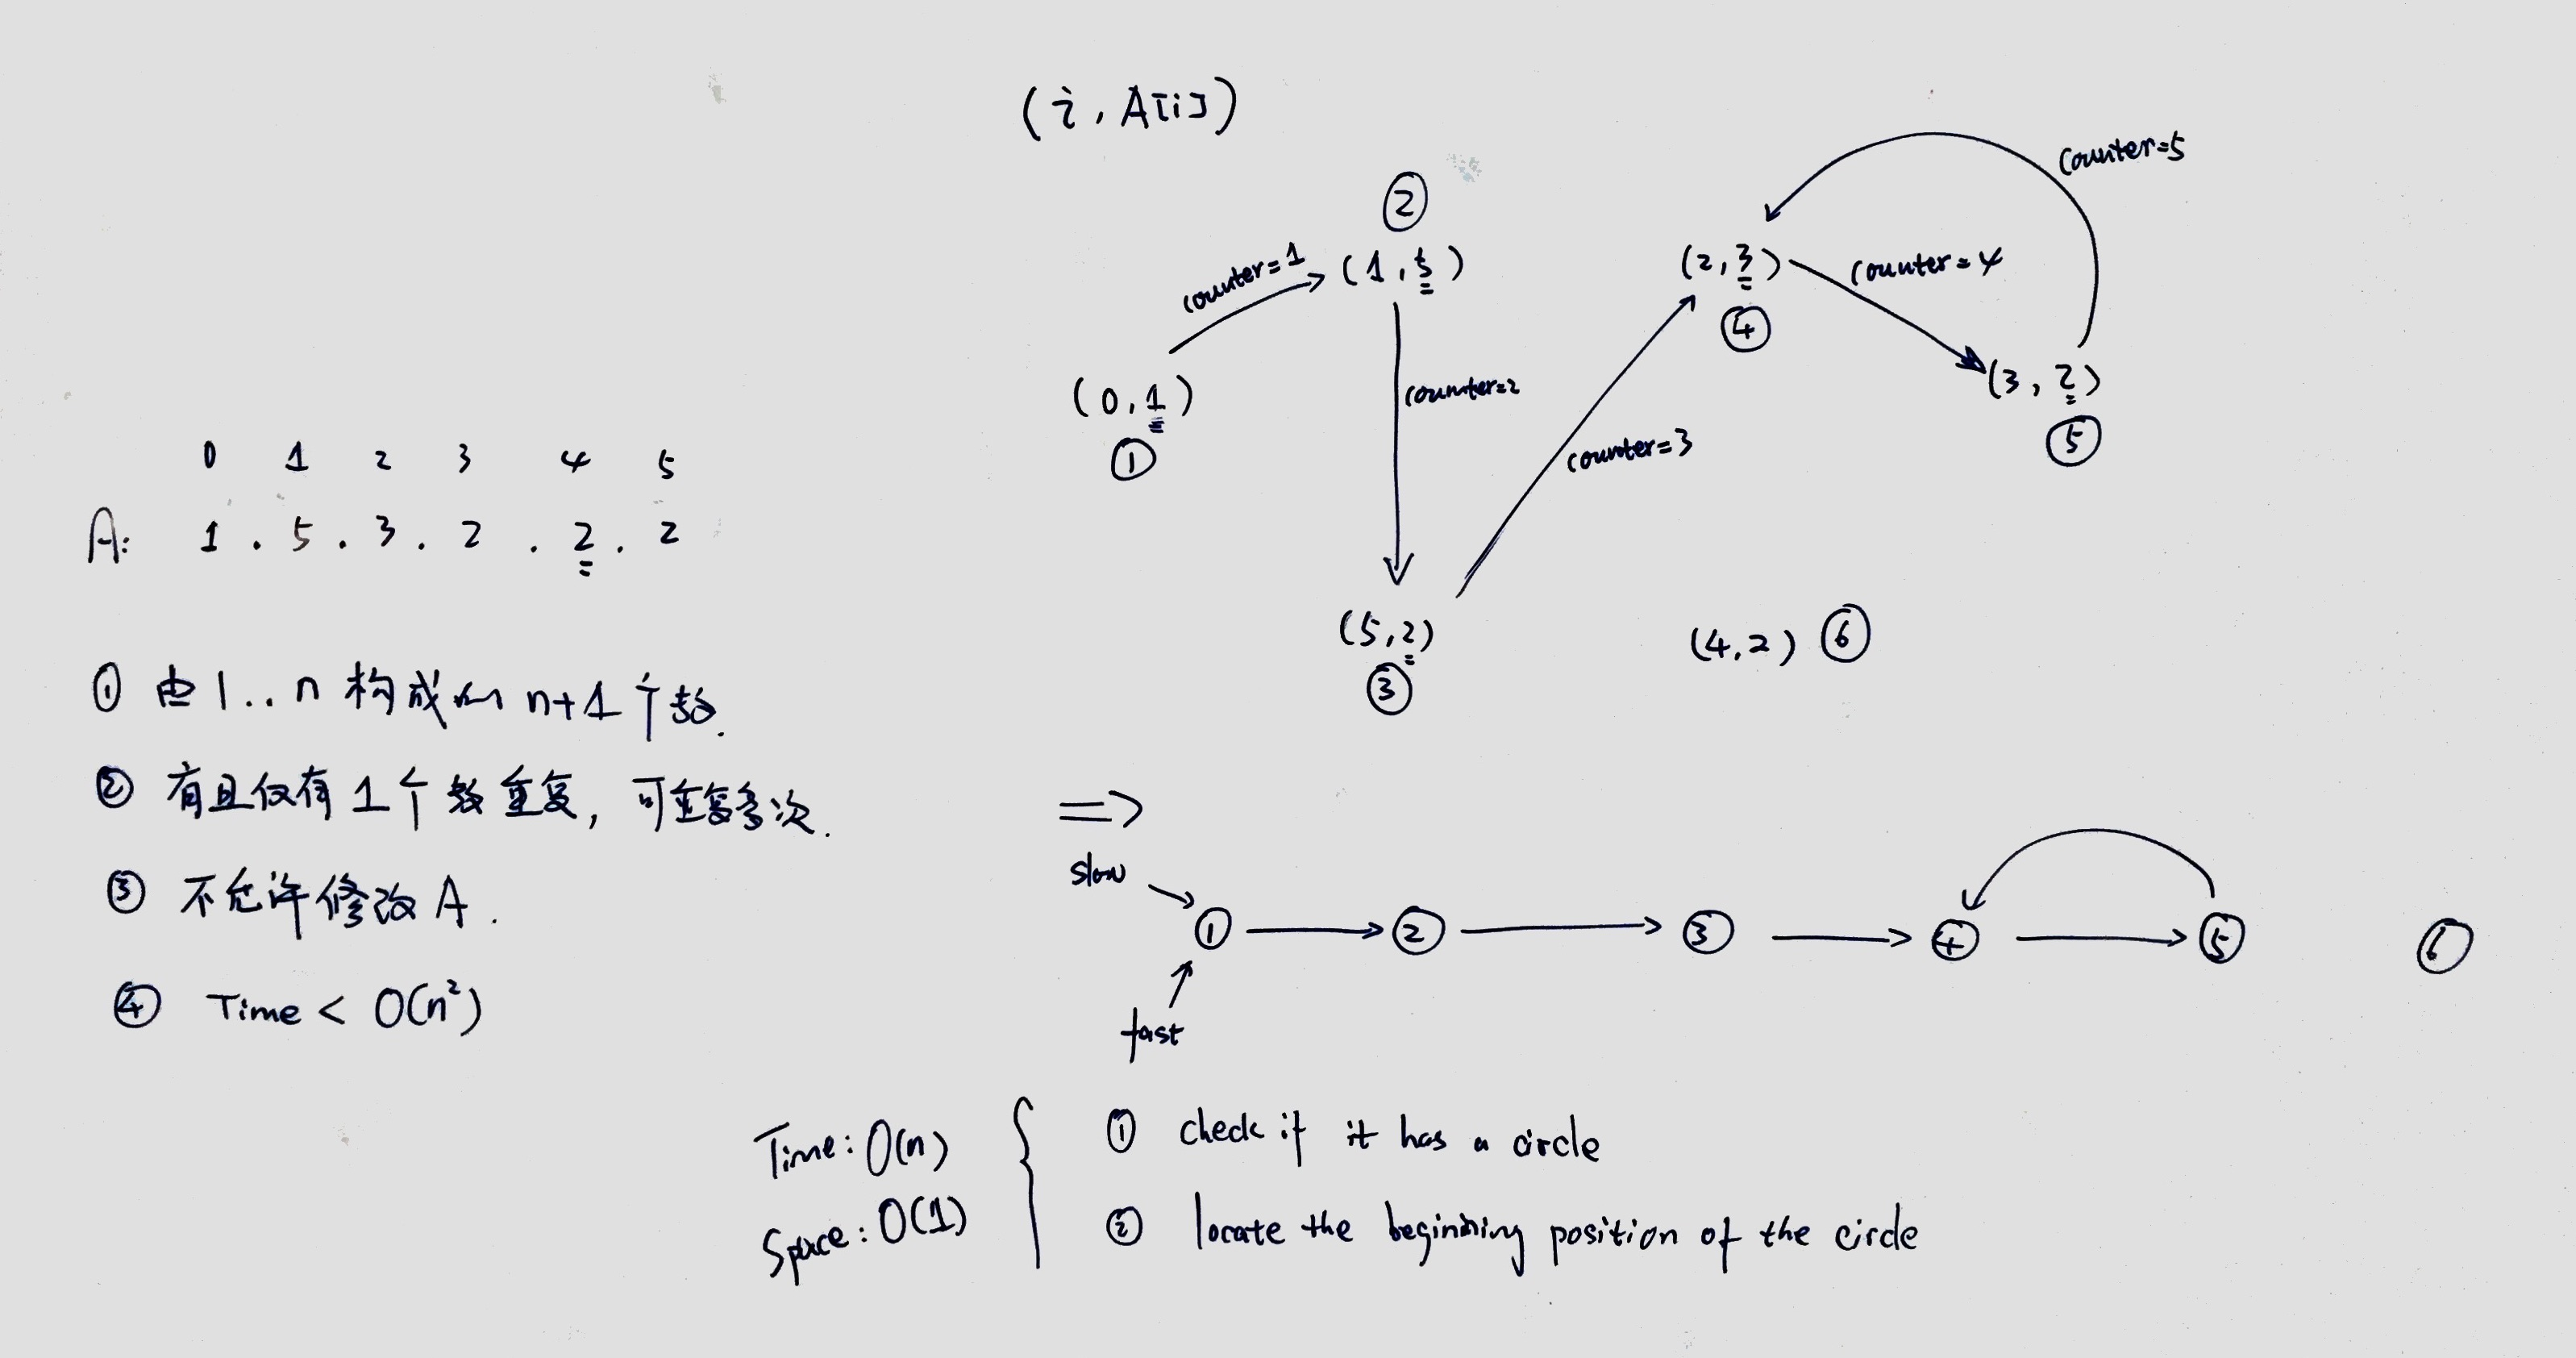
\includegraphics[width=\textwidth]{leetcode287.jpg}
    \centering \\
\end{figure}


\begin{lstlisting}[language=Python, caption=Problem287. Find the Duplicate Number]

class Solution(object):
    # tortoise and hare principle
    def findDuplicate1(self, nums): # RT: O(n)
        # The "tortoise and hare" step.  We start at the end of the array and try
        # to find an intersection point in the cycle.
        slow = 0
        fast = 0
    
        # Keep advancing 'slow' by one step and 'fast' by two steps until they
        # meet inside the loop.
        while True:
            slow = nums[slow]
            fast = nums[nums[fast]]
    
            if slow == fast:
                break
    
        # Start up another pointer from the end of the array and march it forward
        # until it hits the pointer inside the array.
        finder = 0
        while True:
            slow   = nums[slow]
            finder = nums[finder]
    
            # If the two hit, the intersection index is the duplicate element.
            if slow == finder:
                return slow
    
    # binary search + pigeonhold principle
    def findDuplicate2(self, nums): # RT: O(nlogn)
        """
        :type nums: List[int]
        :rtype: int
        """
        left, right = 0, len(nums)-1
        while left <= right:
            mid = (left+right) >> 1
            tmp = sum(x <= mid for x in nums)
            if tmp > mid:
                right = mid-1
            else:
                left = mid+1
        return left
    
    def findDuplicate3(self, nums): # RT: O(nlogn)
        n = len(nums)
        nums.sort()
        for x in xrange(n-1):
            if nums[x] == nums[x+1]:
                return nums[x]
\end{lstlisting}


\subsubsection{leetcode 162. Find Peak Element}
A peak element is an element that is greater than its neighbors. Given an input array where $num[i] \neq num[i+1]$, find a peak element and return its index. \\

\noindent The array may contain multiple peaks, in that case return the index to any one of the peaks is fine. You may imagine that $num[-1] = num[n] = -\infty$.

\noindent For example, in array [1, 2, 3, 1], 3 is a peak element and your function should return the index number 2. \\

\begin{CJK*}{UTF8}{gbsn}
\noindent 解题思路:这道题最直接的解法就是遍历数组,比较相邻的两个数,每次记录较大的数的索引,最后返回记录。这个解法的时间复杂度显然就是$O(n)$。然而搜索某种特殊值时,最高效的算法就是binary search,几乎适用于所有在一堆候选者中(1)找最值(有序的情况下,一次去掉一半),或者(2)满足某种特殊条件的特定值(这种情况下,候选者是有序排列还是无序排列无所谓)。针对本题的两种解法,参考示例图中的演算过程。
\end{CJK*}

\begin{figure}[h]
    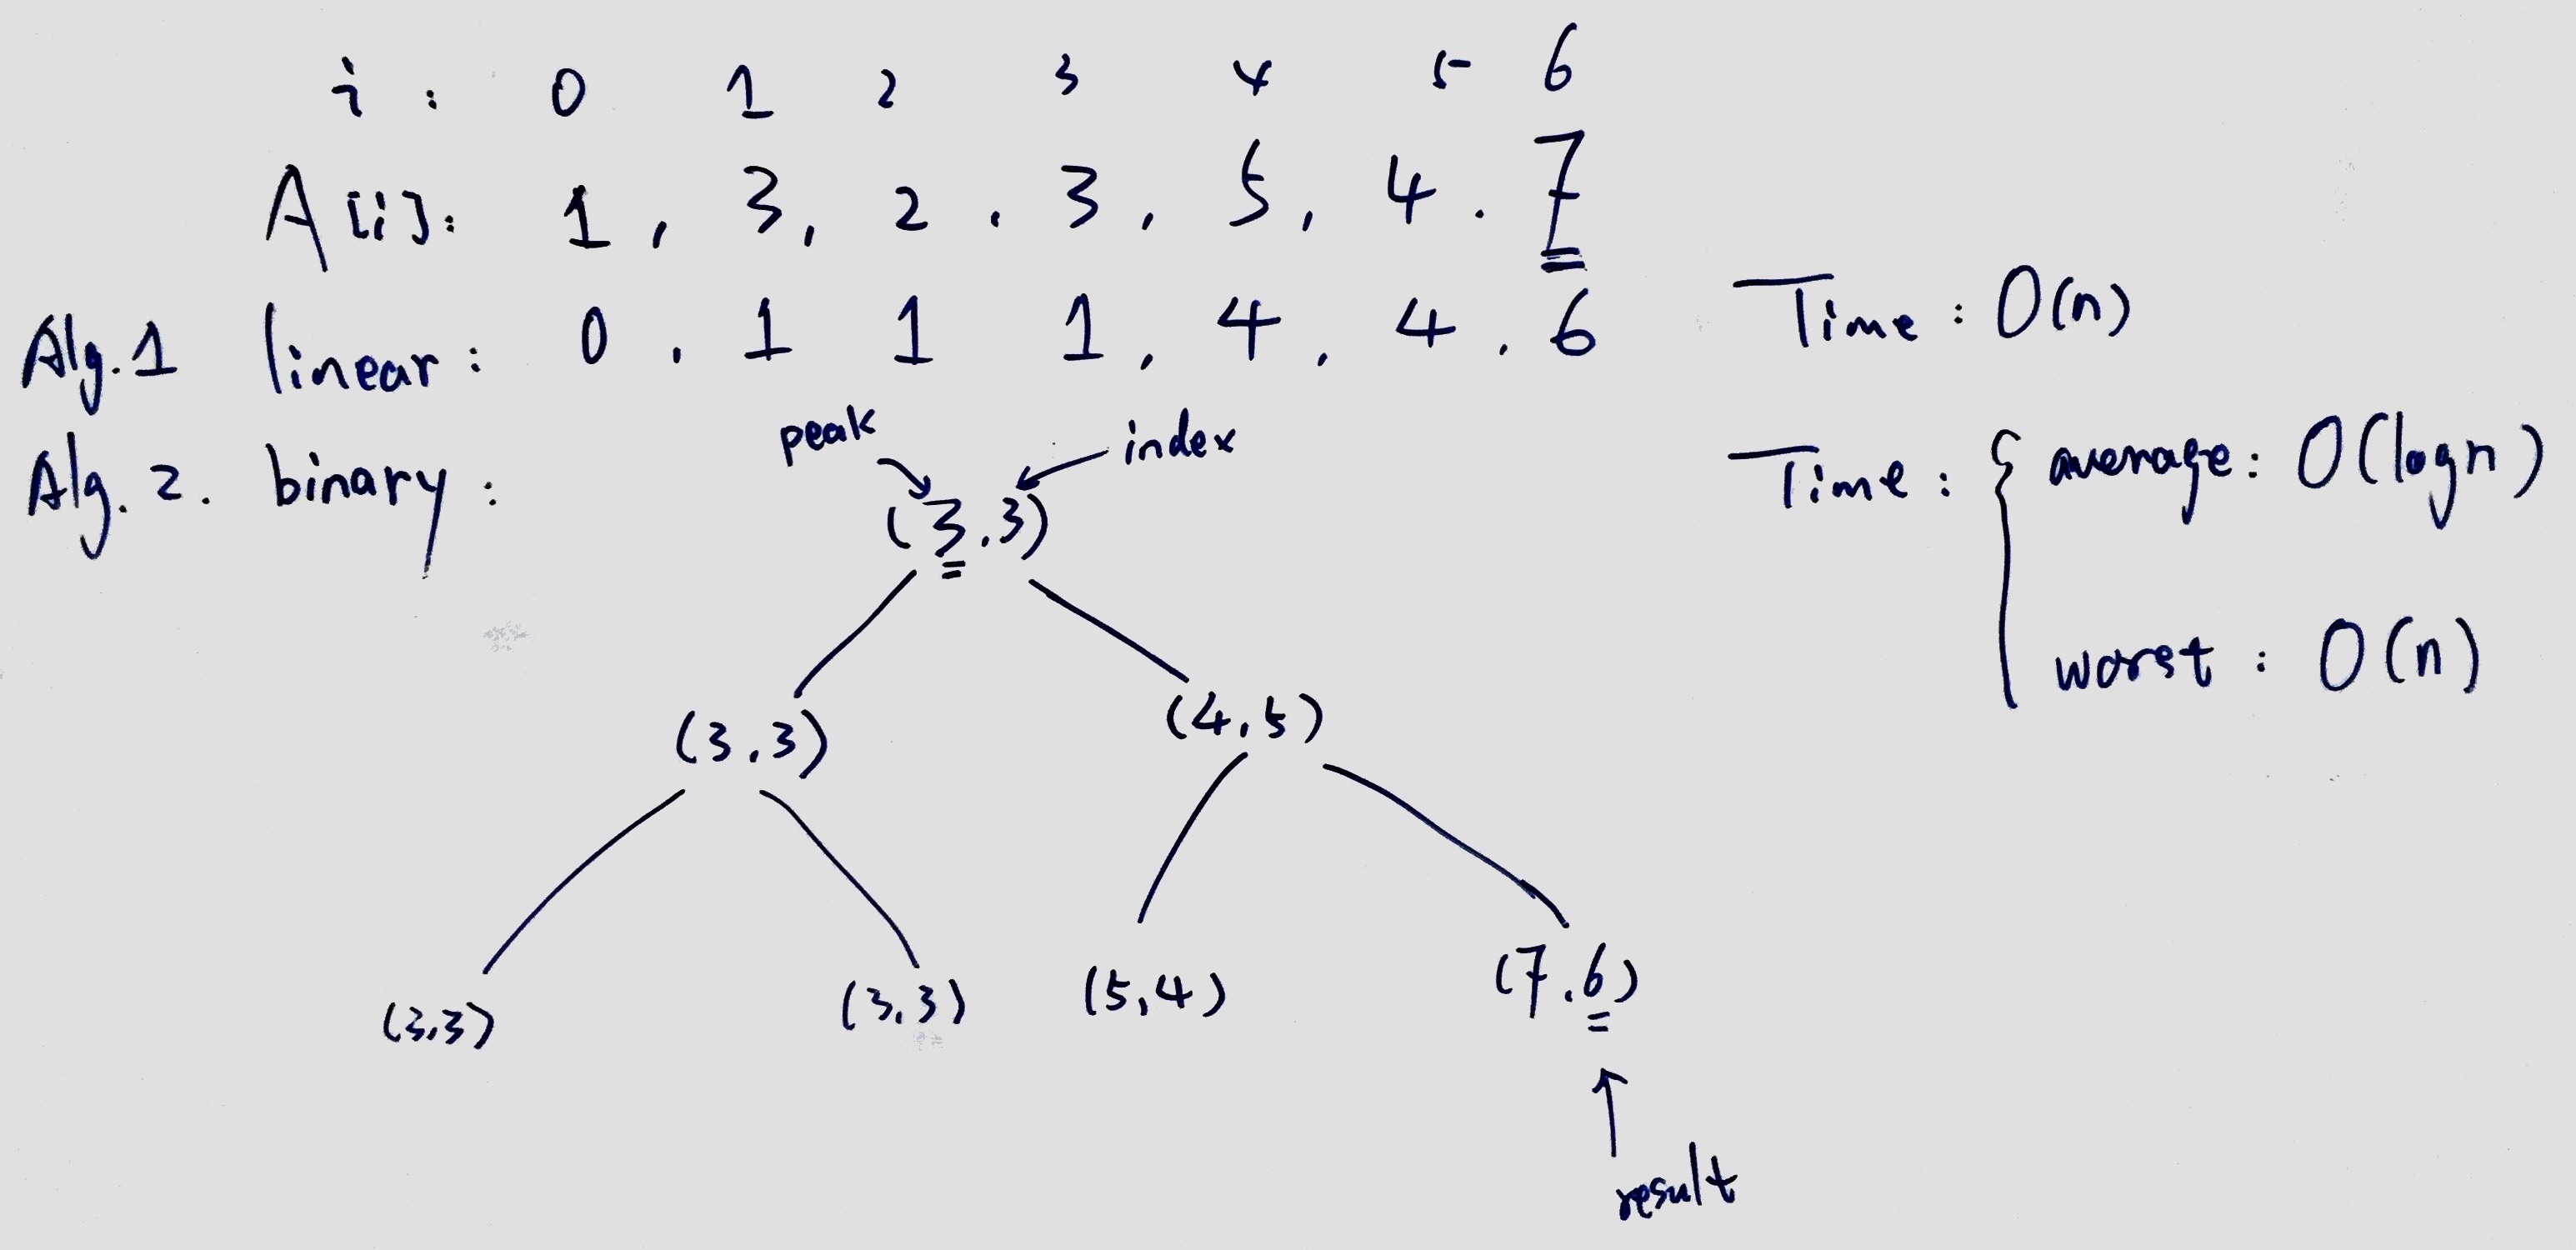
\includegraphics[width=\textwidth]{leetcode162.jpg}
    \centering \\
\end{figure}


\begin{lstlisting}[language=Python, caption=Problem162. Find Peak Element]

class Solution(object):
    def findPeakElement_BS(self, nums):  # RT: O(logn)
        size = len(nums)
        return self.search(nums, 0, size - 1)

    def search(self, nums, start, end):
        if start == end:
            return start
        if start + 1 == end:
            if nums[start] < nums[end]:
                return end
            else:
                return start
        mid = (start + end) / 2
        if nums[mid] < nums[mid - 1]:
            return self.search(nums, start, mid - 1)
        if nums[mid] < nums[mid + 1]:
            return self.search(nums, mid + 1, end)
        return mid

    def findPeakElement_traverse(self, nums):  # RT: O(n)
        """
        :type nums: List[int]
        :rtype: int
        """
        n = len(nums)
        for i in range(1, n-1):
            if nums[i-1] < nums[i] and nums[i] > nums[i+1]:
                return i
        if nums[0] < nums[n-1]:
            return n-1
        else:
            return 0
\end{lstlisting}






























%%%%%%%%%%%%%%%%%%%%%%%%%%%%%%%%%%%%%%%%%%%%%%%%%%%%%%%%%%%%%%%%%%%%%%%%%
%%%%%%%%%%%%%%%%%%%%%%%%  Linked List %%%%%%%%%%%%%%%%%%%%%%%%%%%%%%%%%%%
%%%%%%%%%%%%%%%%%%%%%%%%%%%%%%%%%%%%%%%%%%%%%%%%%%%%%%%%%%%%%%%%%%%%%%%%%

\subsection{Singly Linked List}

\subsubsection{leetcode 328. Odd Even Linked List}
Given a singly linked list, group all odd nodes together followed by the even nodes. Please note here we are talking about the node number and not the value in the nodes. You should try to do it \textbf{in place}. The program should run in $O(1)$ space complexity and $O(n)$ time complexity. \\

\noindent Example: Given 1->2->3->4->5->NULL, return 1->3->5->2->4->NULL.

\noindent Note: The relative order inside both the even and odd groups should remain as it was in the input. The first node is considered odd, the second node even and so on ... \\

\begin{CJK*}{UTF8}{gbsn}
\noindent 解题思路:根据题目要求,需要原地进行,因此考查的内容是指针的操作。解题方法是使用原有链表的头结点作为奇数结点链表的头结点,使用原链表第一个偶数结点作为偶数结点链表的头结点。用两个额外的指针分别指向奇数、偶数结点链表的头结点,每次移动两步,分别读取奇、偶结点;最后再将偶数结点链表插入到奇数结点链表的尾部,即可。参考下面示例图中的演示。
\end{CJK*}

\begin{figure}[h]
    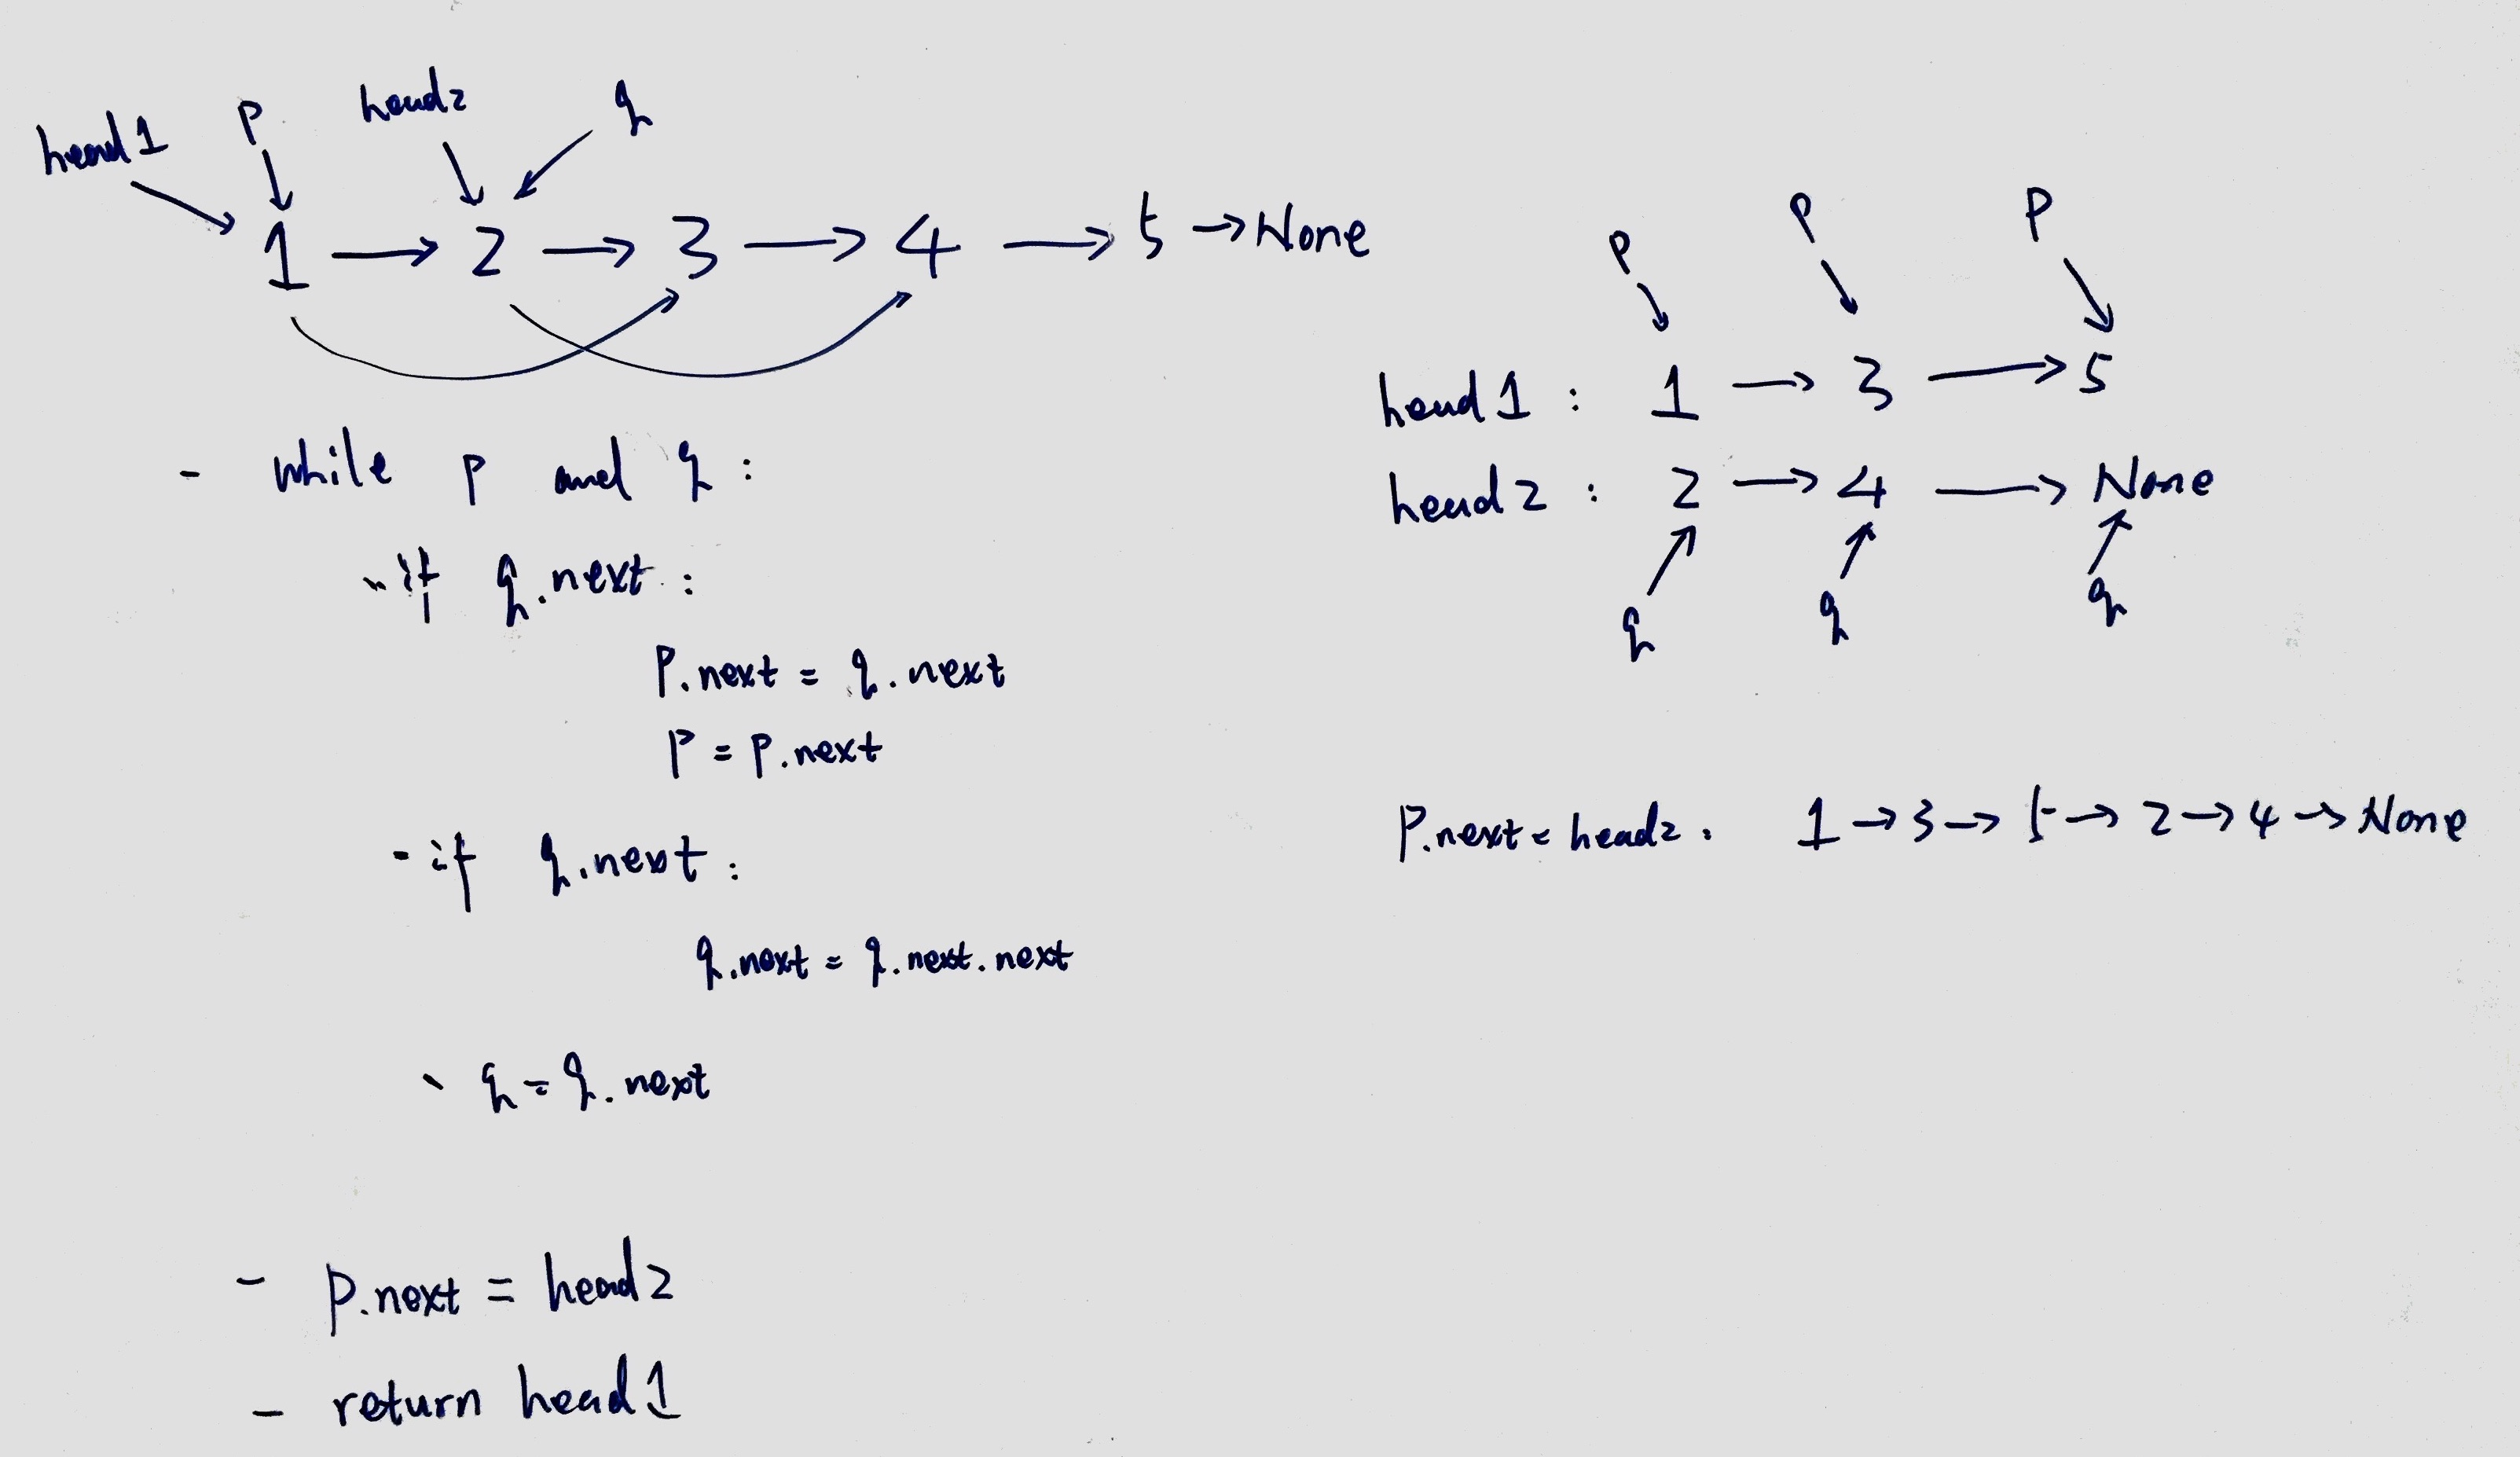
\includegraphics[width=\textwidth]{leetcode328.jpg}
    \centering \\
\end{figure}

\begin{lstlisting}[language=Python, caption=Problem328. Odd Even Linked List]

# Definition for singly-linked list.
# class ListNode(object):
#     def __init__(self, x):
#         self.val = x
#         self.next = None

class Solution(object):
    if head is None or head.next is None:
            return head
        oddPtr = head
        evenHead = evenPtr = head.next
        while oddPtr and evenPtr:
            if evenPtr.next:
                oddPtr.next = evenPtr.next
                oddPtr = oddPtr.next
            if evenPtr.next:
                evenPtr.next = evenPtr.next.next
            evenPtr = evenPtr.next
        oddPtr.next = evenHead
        return head
\end{lstlisting}


\subsubsection{leetcode 2. Add Two Numbers}
You are given two linked lists representing two non-negative numbers. The digits are stored in \textbf{reverse order} and each of their nodes contain a single digit. Add the two numbers and return it as a linked list. \\

\noindent For example: \\
\indent Input: (2 -> 4 -> 3) + (5 -> 6 -> 4) \\
\indent Output: 7 -> 0 -> 8 \\

\begin{CJK*}{UTF8}{gbsn}
\noindent 解题思路:这道题与leetcode 66 Plus One类似,差别在于后者是考查数组。有两点需要注意:一是进位的处理:需要一个额外的变量carry记录每次加法以后是否有进位;二是计算到其中一个链表的末尾时,如果有进位情况发生(carry=1),那么要么累加到更长的那个链表上去,要么就创建一个新结点并添加到结果链表的尾部。下面的示例图是添加一个新的链表结点到结果链表的尾部。另外需要注意的,在处理数组加法的题目时,可以先判断两个数组的结点数目。结点数目多的链表,可用作最后的结果链表。但是,需要进行一次遍历才能判断哪个链表包含更多的结点。这个方法适合于in-place类型的任务。\\
\end{CJK*}


\begin{lstlisting}[language=Python, caption=Problem2. Add Two Numbers]

# Definition for singly-linked list.
# class ListNode(object):
#     def __init__(self, x):
#         self.val = x
#         self.next = None

class Solution(object):
    def addTwoNumbers(self, l1, l2): # RT: O(max{len(l1),len(l2)})
        """
        :type l1: ListNode
        :type l2: ListNode
        :rtype: ListNode
        """
        if l1 == None: return l2
        if l2 == None: return l1

        h1 = l1; h2 = l2
        while h1!=None and h2!=None:
            h1 = h1.next
            h2 = h2.next
        if h2!=None: l1,l2 = l2,l1

        head = l1
        carry = 0
        while l2!=None:
            asum = l1.val + l2.val + carry
            l1.val = asum%10
            carry = asum/10
            # l1 and l2 have same size
            if l2.next is None and l1.next is None and carry==1:
                l1.next = ListNode(carry)
                carry = 0
            l1 = l1.next
            l2 = l2.next

        while carry==1 and l1:
            asum = carry + l1.val
            l1.val = asum%10
            carry = asum/10
            if l1.next is None and carry==1:
                l1.next = ListNode(carry)
                break
            l1 = l1.next
        return head
\end{lstlisting}

\begin{figure}[h]
    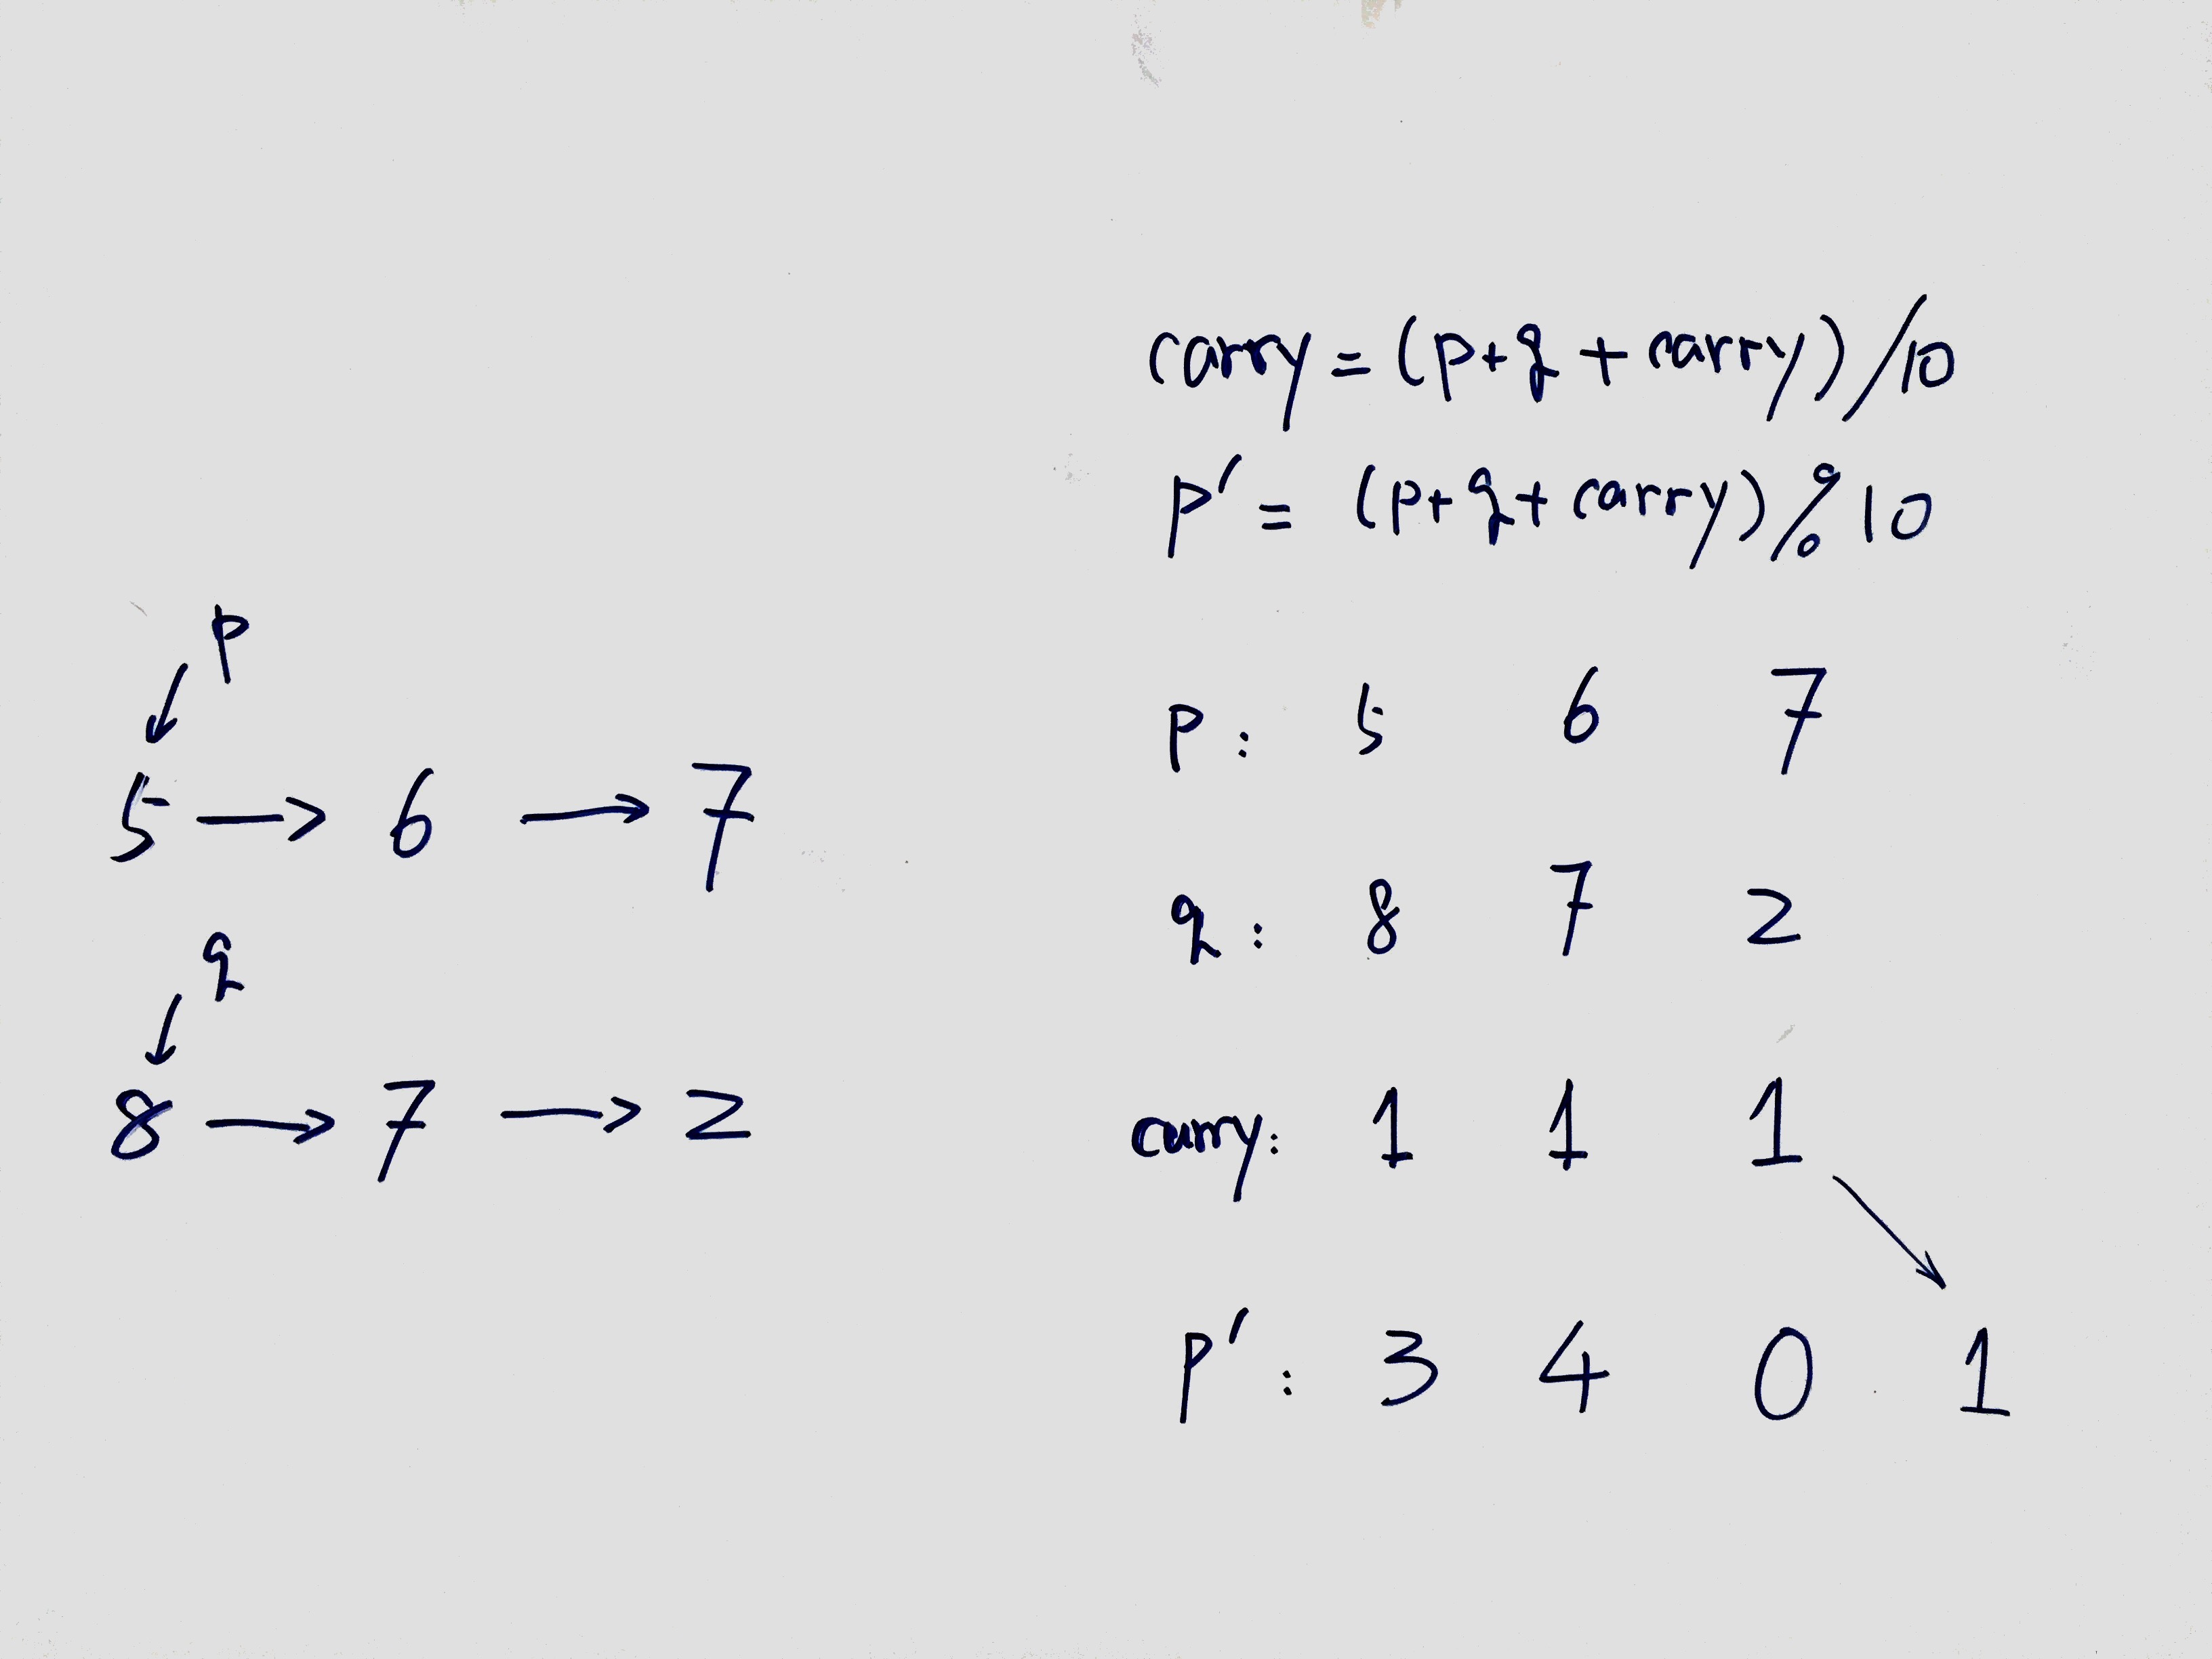
\includegraphics[width=\textwidth]{leetcode2.jpg}
    \centering \\
\end{figure}



\subsubsection{leetcode 92. Reverse Linked List II}
Reverse a linked list from position $m$ to $n$. Do it in-place and in one-pass. \\

\noindent For example: \\
\indent Given 1->2->3->4->5->NULL, m = 2 and n = 4, \\
\indent return 1->4->3->2->5->NULL. \\

\noindent Note: \\
\indent Given m, n satisfy the following condition: $1 \leq m \leq n \leq $length of list. \\

\begin{CJK*}{UTF8}{gbsn}
\noindent 解题思路:反转链表考查的是对单链表指针的基本操作。这道题有三个地方需要注意:第一点是确定反转区间的开始结点$m$。但是实际算法中,需要始终保存的结点不是$m$结点,而是其前驱结点$m-1$。$m-1$结点可以用于定位反转区间的开始结点以外,还可以在反转任务结束后,便于穿入反转后的区间链表。第二个需要注意的地方是单链表反转技巧:需要使用到三个辅助指针pre, curr, next。pre和curr用于反转两个结点之间的指针,并且用curr更新pre;next则用于反转后更新curr指向下一个结点。当curr指向结点$n$的时候,反转工作结束;之后,将结点$m-1$的next指针当前所指向的结点($m$)的next指针指向next指针当前指向的结点,再将结点$m-1$的next指针指向curr当前指向的结点即完成整个任务。参考下面的示例图。第三个值得注意的地方,因为反转的起点很可能是链表的第一个结点,所以为了保证算法的通用性,可以增加一个伪头结点dummy。
\end{CJK*}

\begin{figure}[h]
    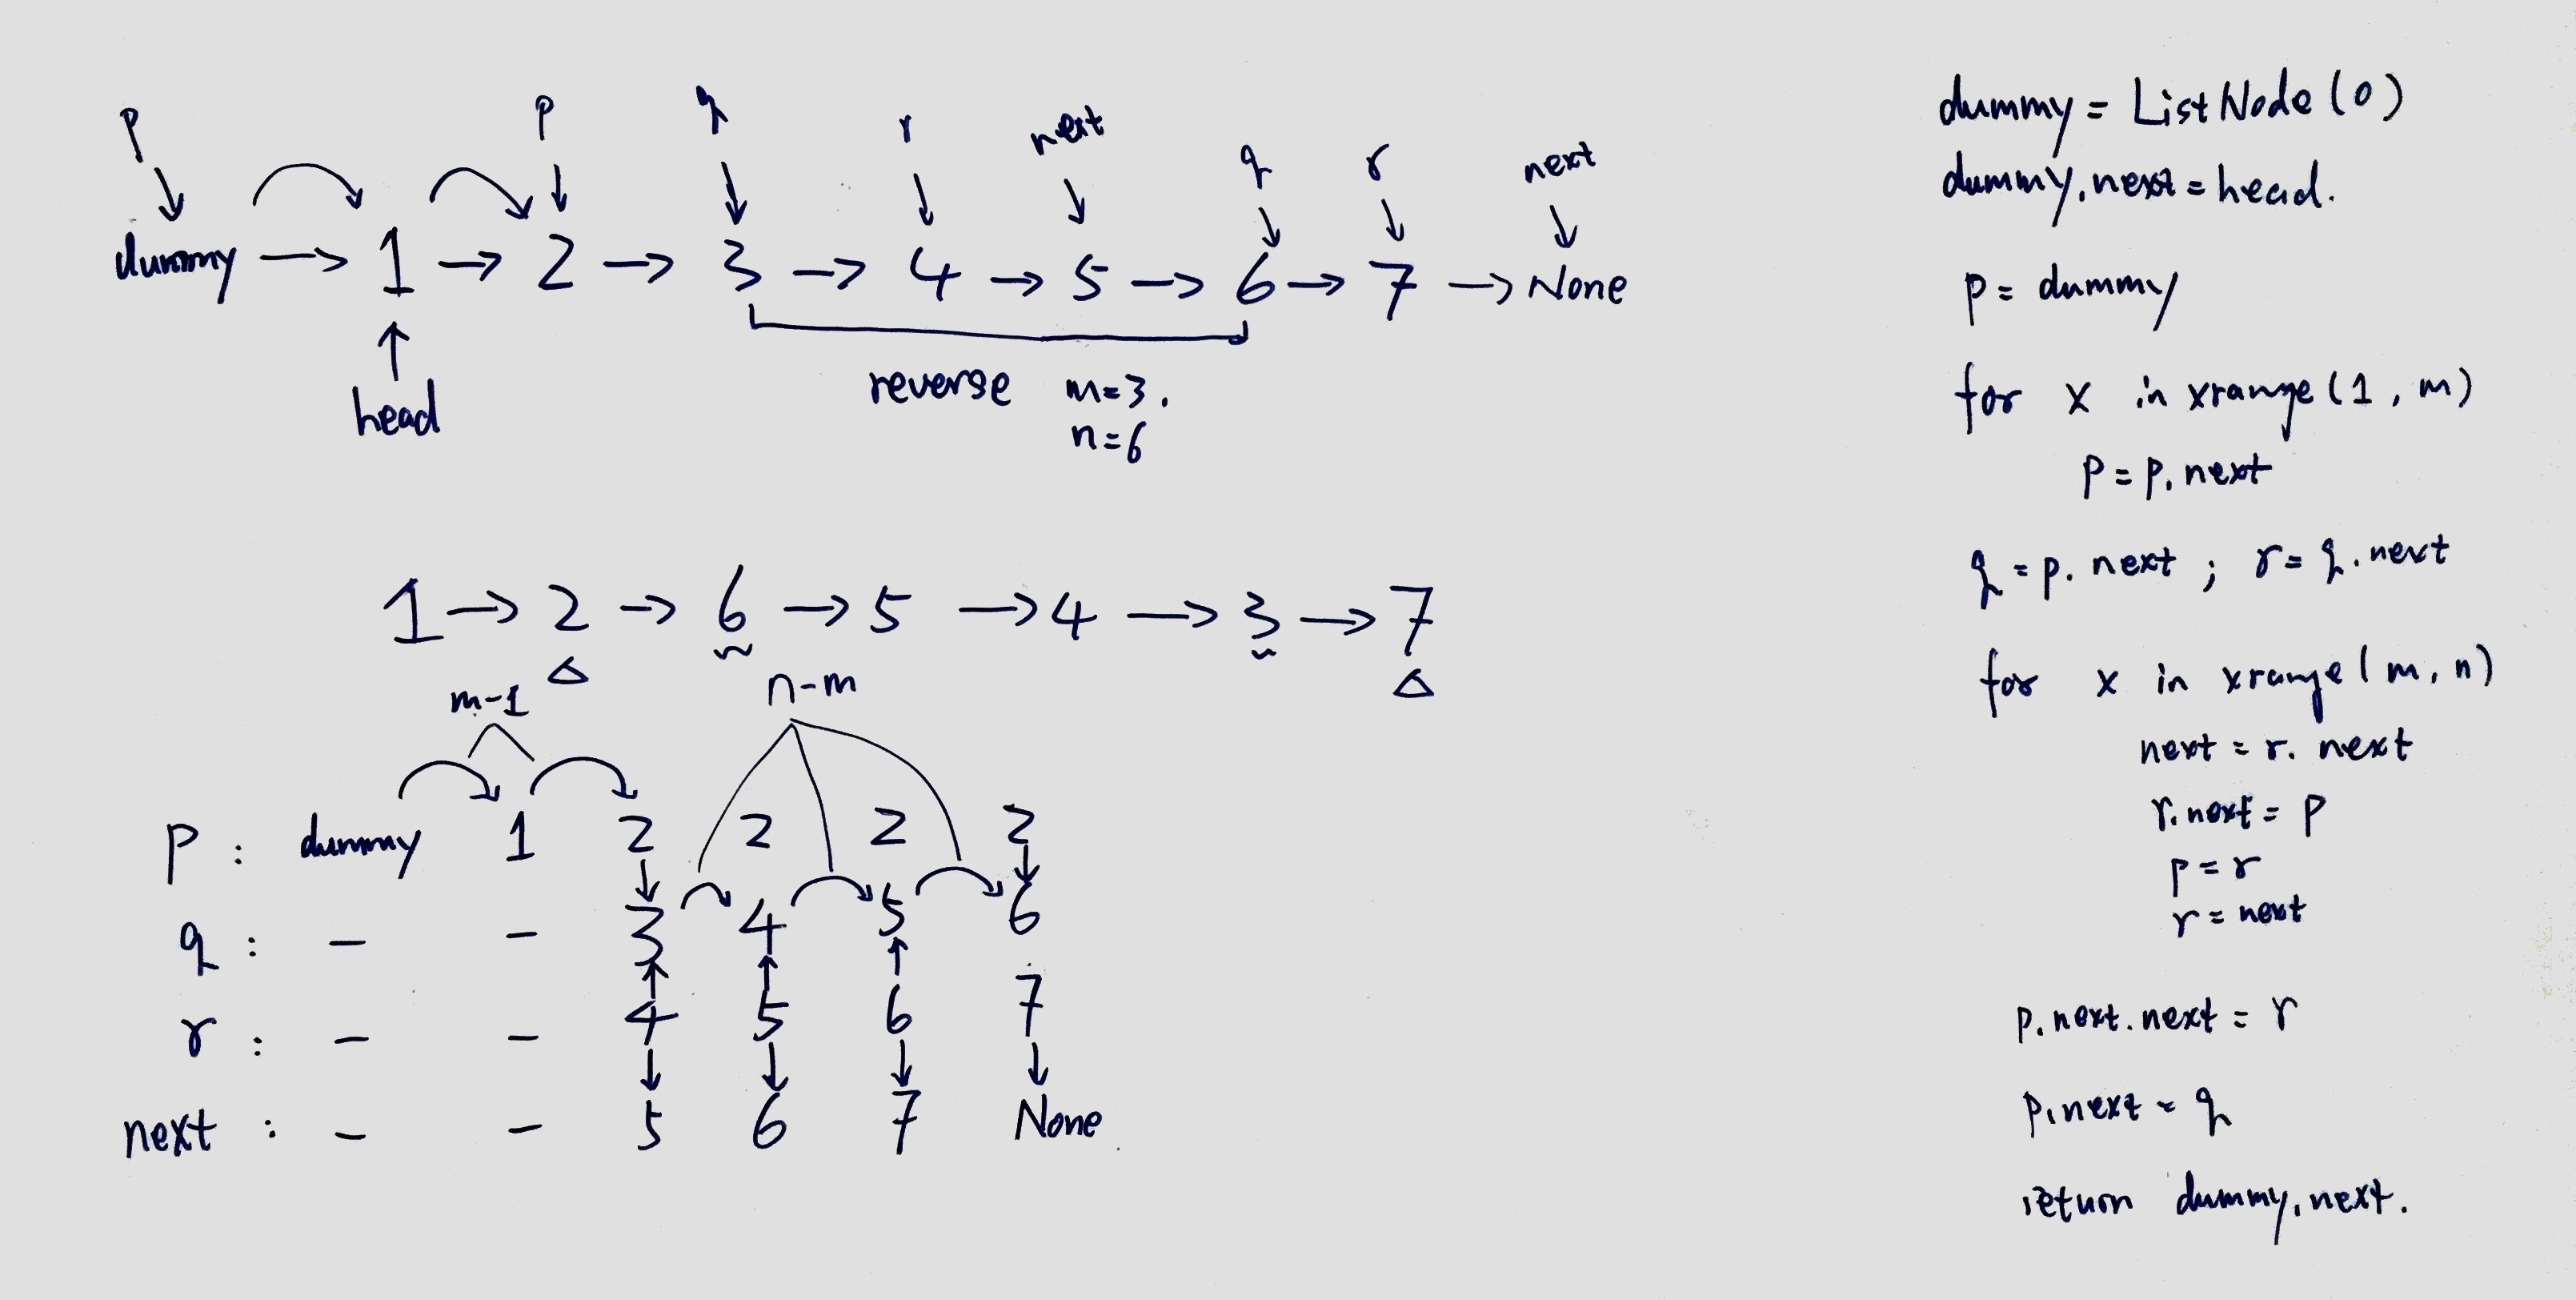
\includegraphics[width=\textwidth]{leetcode92.jpg}
    \centering \\
\end{figure}

\begin{lstlisting}[language=Python, caption=Problem92. Reverse Linked List II]

def reverseBetween(self, head, m, n): # RT: O(n)
        """
        :type head: ListNode
        :type m: int
        :type n: int
        :rtype: ListNode
        """
        def reverseBetween(self, head, m, n):
        if head==None or head.next==None: return head
        dummy = ListNode(0)
        dummy.next = head
        p = dummy
        for x in xrange(m-1):
            p = p.next
        q = p.next # q is the m-th node
        r = q.next
        for x in xrange(m, n):
            tmp = r.next
            r.next = q
            q = r
            r = tmp
        p.next.next = r
        p.next = q
        return dummy.next
\end{lstlisting}


\subsubsection{leetcode 86. Partition List}
Given a linked list and a value $x$, partition it such that all nodes less than $x$ come before nodes greater than or equal to $x$. You should preserve the \textbf{original relative order} of the nodes in each of the two partitions. \\

\noindent For example, \\
\indent Given 1->4->3->2->5->2 and x = 3,\\
\indent return 1->2->2->4->3->5. \\

\begin{CJK*}{UTF8}{gbsn}
\noindent 解题思路:这道题的算法的设计思路与leetcode328几乎一直。考查的点依然是对单链表这种数据结构指针部分的基本操作。
\end{CJK*}

\begin{lstlisting}[language=Python, caption=Problem86. Partition List]

# Definition for singly-linked list.
# class ListNode(object):
#     def __init__(self, x):
#         self.val = x
#         self.next = None

class Solution(object):
    def partition(self, head, x):
        """
        :type head: ListNode
        :type x: int
        :rtype: ListNode
        """
        if head==None or head.next==None: return head
        dummy = ListNode(0)
        dummy.next = head
        ghead = gtail = ListNode(0)
        ltail = dummy
        p = dummy.next
        while p:
            if p.val < x:
                ltail.next = p
                p = p.next
                ltail = ltail.next
            else:
                gtail.next = p
                p = p.next
                gtail = gtail.next
        ltail.next = ghead.next
        gtail.next = None
        return dummy.next
\end{lstlisting}



\subsubsection{leetcode 83. Remove Duplicates from Sorted List}
Given a sorted linked list, delete all duplicates such that each element appear only once. \\

\noindent For example,\\
\indent Given 1->1->2, return 1->2. \\
\indent Given 1->1->2->3->3, return 1->2->3. \\

\begin{CJK*}{UTF8}{gbsn}
\noindent 解题思路:这道题与数组题目的leetcode26在算法方面的考核点几乎一致。唯一不同的就是问题针对的是不同的数据结构。解题思路就是使用快慢指针的设计方法:快慢指针每次向前移动一个结点,如果两个指针指向的结点具有相同数值,停止移动慢指针;如果两个指针指向的结点具有不同的数值,则慢指针向前移动一个结点,然后拷贝快指针指向的结点数值到慢指针当前的结点;拷贝结束后再继续上述过程。具体示例参考下面示例图。
\end{CJK*}

\begin{figure}[h]
    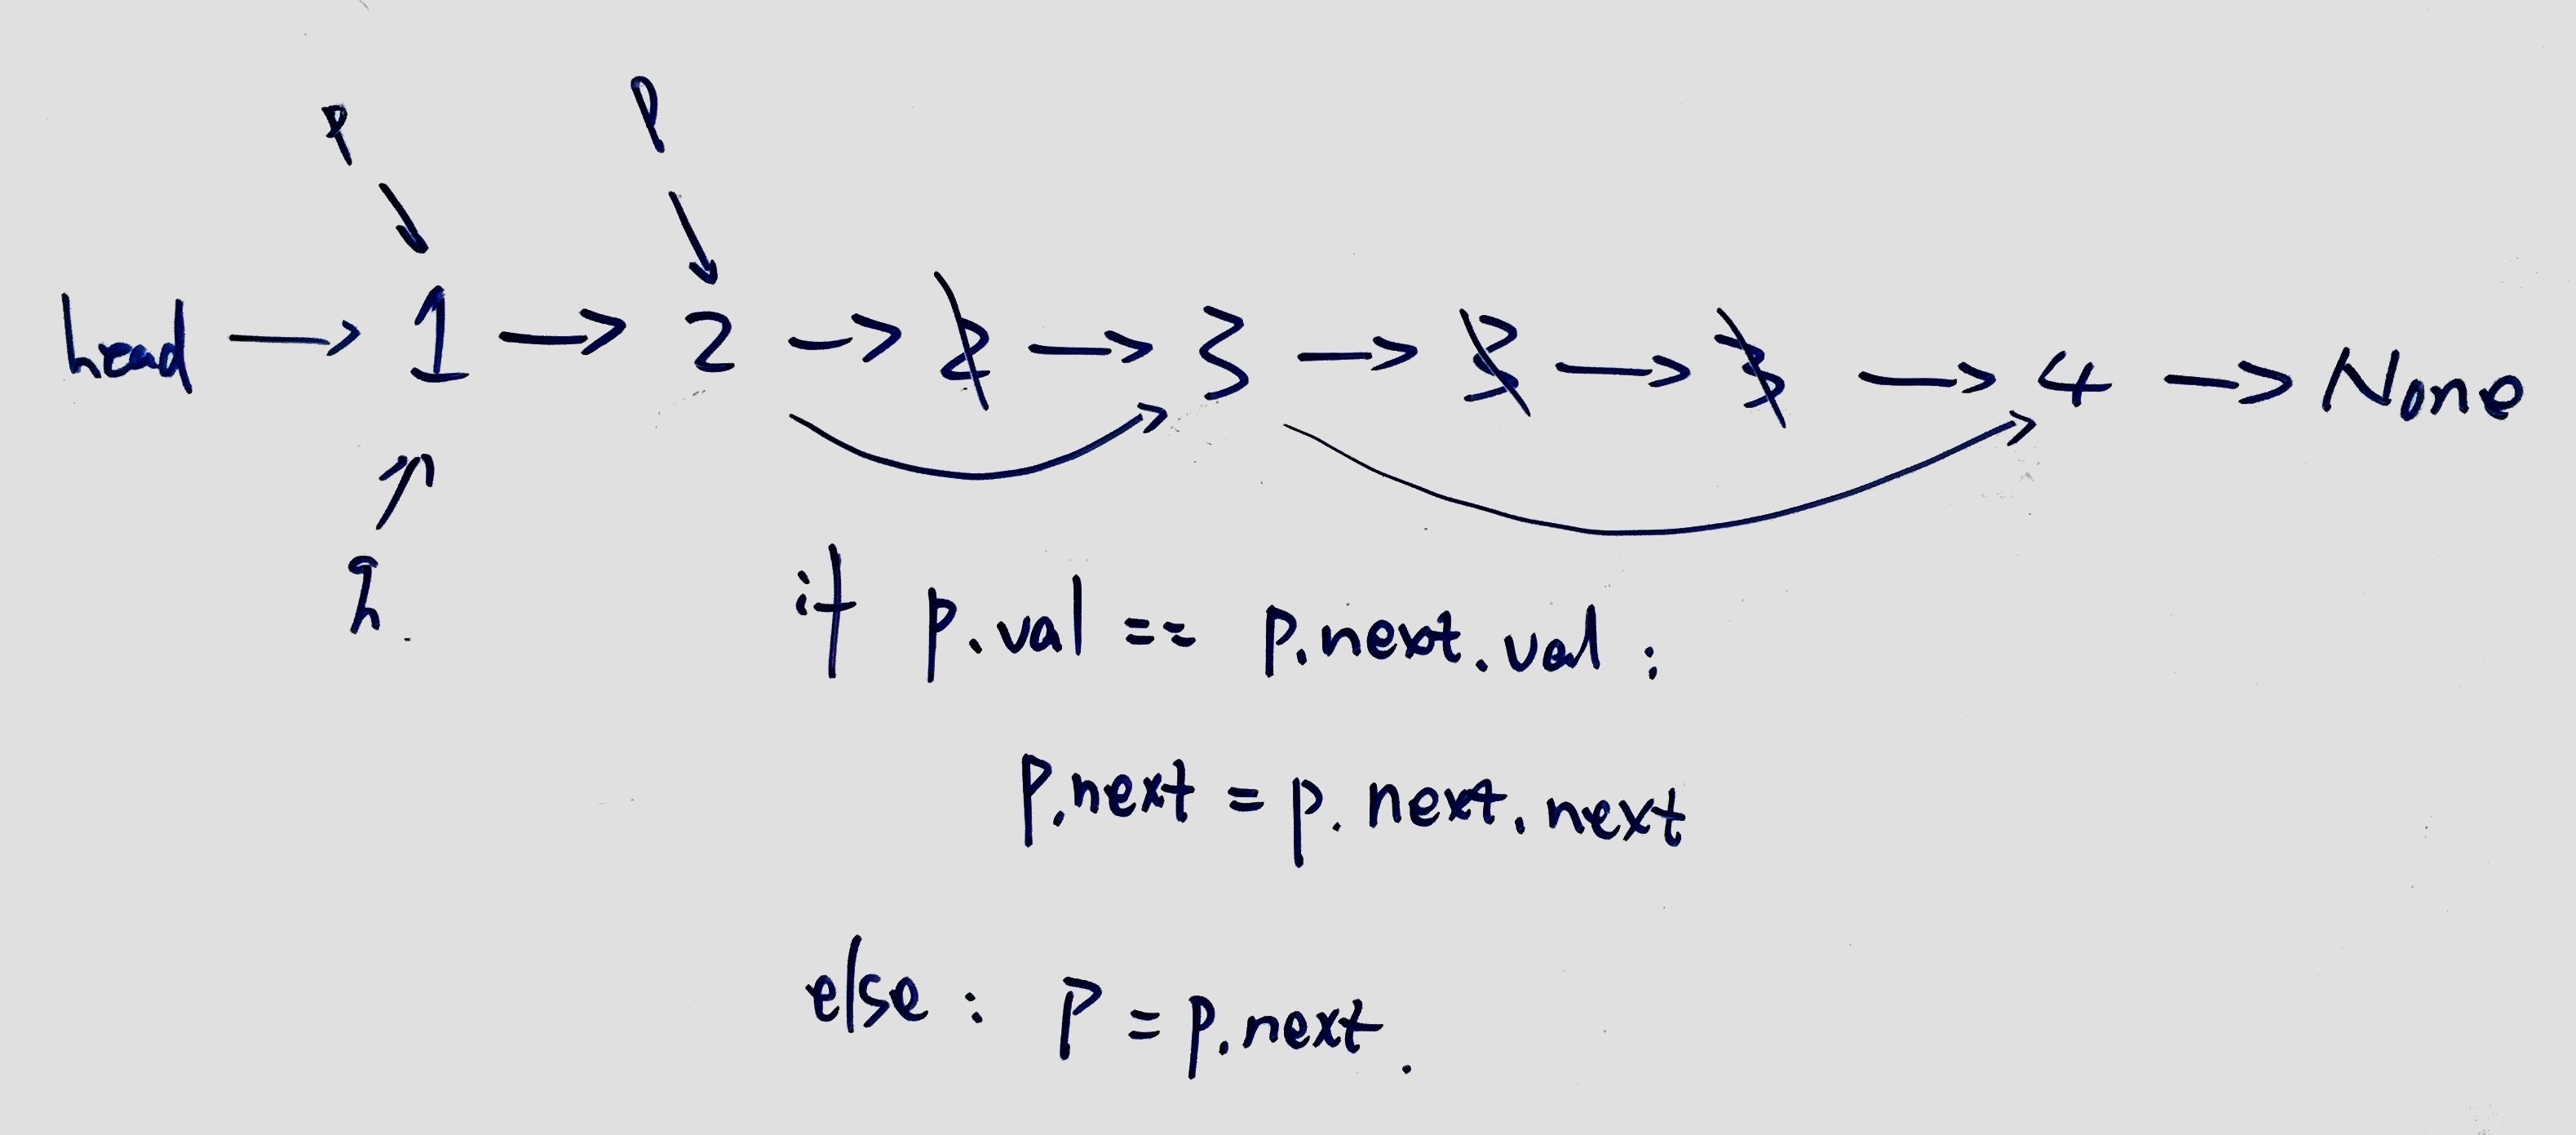
\includegraphics[width=\textwidth]{leetcode83.jpg}
    \centering \\
\end{figure}

\begin{lstlisting}[language=Python, caption=Problem83. Remove Duplicates from Sorted List]

# Definition for singly-linked list.
# class ListNode(object):
#     def __init__(self, x):
#         self.val = x
#         self.next = None

class Solution(object):
    def deleteDuplicates(self, head):
        """
        :type head: ListNode
        :rtype: ListNode
        """
        fast = head
        while fast != None and fast.next != None:
            if fast.val == fast.next.val:
                curr = fast
                while fast!=None and fast.val==curr.val:
                    fast = fast.next
                curr.next = fast
            else:
                fast = fast.next
        return head
\end{lstlisting}


\subsubsection{leetcode 82. Remove Duplicates from Sorted List II}
Given a sorted linked list, delete all nodes that have duplicate numbers, leaving only distinct numbers from the original list.\\

\noindent For example,\\
\indent Given 1->2->3->3->4->4->5, return 1->2->5. \\
\indent Given 1->1->1->2->3, return 2->3. \\

\begin{lstlisting}[language=Python, caption=Problem82. Remove Duplicates from Sorted List II]

# Definition for singly-linked list.
# class ListNode(object):
#     def __init__(self, x):
#         self.val = x
#         self.next = None

class Solution(object):
    def deleteDuplicates(self, head):
        if head==None or head.next==None: return head
        dummy = ListNode(0)
        dummy.next = head
        pre, curr, next = dummy, head, head.next
        while next:
            if curr.val != next.val:
                next = next.next
                curr = curr.next
                pre = pre.next
            else:
                while next and next.val==curr.val:
                    next = next.next
                curr = next
                pre.next = curr
                if next: next = next.next
                else: break
        return dummy.next
\end{lstlisting}



\subsubsection{leetcode 61. Rotate List}
Given a list, rotate the list to the right by k places, where k is non-negative. \\

\noindent For example, given 1->2->3->4->5->NULL and k = 2, \\
\indent return 4->5->1->2->3->NULL. \\

\begin{CJK*}{UTF8}{gbsn}
\noindent 解题思路:因为第$k$个位置是从右侧算的,所以需要定位到这个位置。定位的方法是使用快慢指针:快指针先走$k$步,然后再同时移动快、慢指针;当快指针到达最后一个结点时,慢指针指向的结点即为结果链表的尾结点;而慢指针指向的结点的下一个结点即是结果链表的头结点,将快指针指向的结点的next指针指向原来的头结点即得到最终的结果。此外,$k$可能大于链中节点的总数$n$,所以在计算节点总数之后要进行处理:$k=k\%n$。参考下面的示例图。\\
\end{CJK*}


\begin{lstlisting}[language=Python, caption=Problem61. Rotate List]

# Definition for singly-linked list.
# class ListNode(object):
#     def __init__(self, x):
#         self.val = x
#         self.next = None

class Solution(object):
    def rotateRight(self, head, k):  # RT: O(n)
        """
        :type head: ListNode
        :type k: int
        :rtype: ListNode
        """
        if head == None or head.next == None:
            return head

        fast = head
        n = 1
        # compute the length of the linked list
        while fast.next:
            fast = fast.next
            n += 1

        k = k % n
        slow = fast = head
        step = 0
        while step < k:
            fast = fast.next
            step += 1

        while fast.next:
            fast = fast.next
            slow = slow.next

        fast.next = head
        head = slow.next
        slow.next = None
        return head
\end{lstlisting}

\begin{figure}[h]
    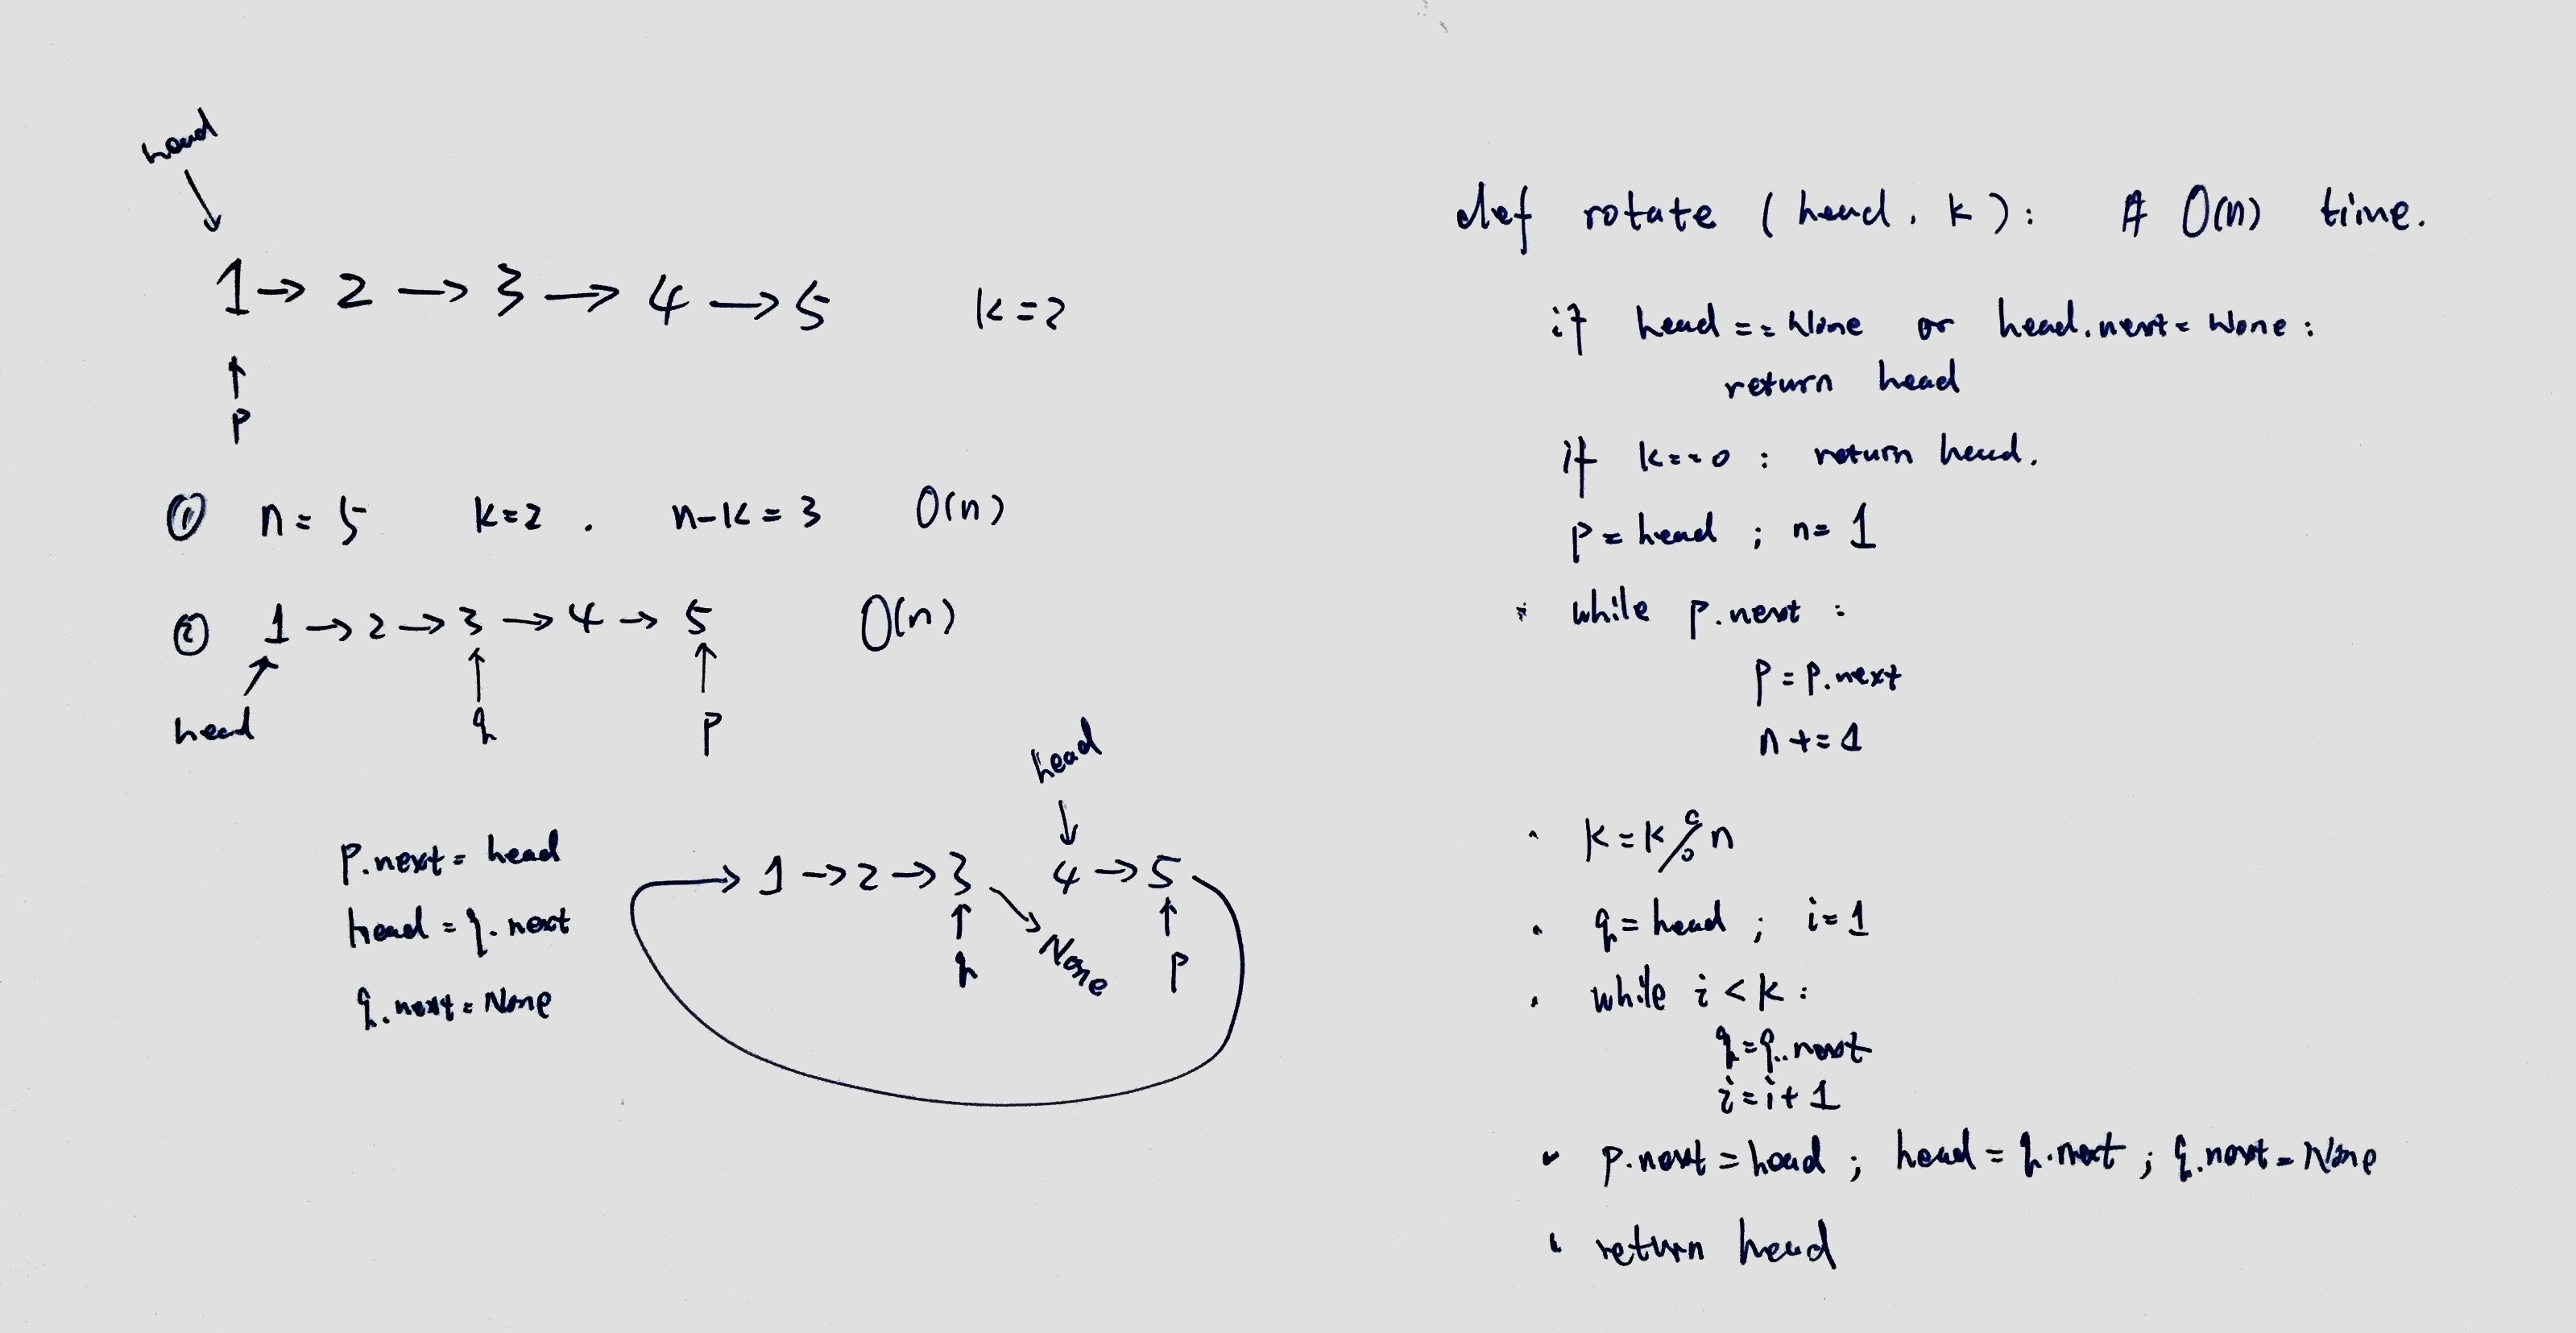
\includegraphics[width=\textwidth]{leetcode61.jpg}
    \centering \\
\end{figure}




\subsubsection{leetcode 19. Remove $n^{th}$ Node From End of List}
Given a linked list, remove the $n^{th}$ node from the end of list and return its head. For example, given linked list: 1->2->3->4->5, and n = 2. \\
\indent After removing the second node from the end, the linked list becomes 1->2->3->5. \\

\begin{CJK*}{UTF8}{gbsn}
\noindent 解题思路:这道题依然是使用快慢指针法:首先,向前移动快指针$n$步;然后,再同时移动快慢指针,是的快慢指针之间始终保持$n$步;当快指针到达链表最后一个结点时,慢指针指向倒数第$n+1$个结点;最后,直接将慢指针所指向结点的next指针指向倒数第$n-1$个结点即完成删除任务。
\end{CJK*}

\begin{figure}[h]
    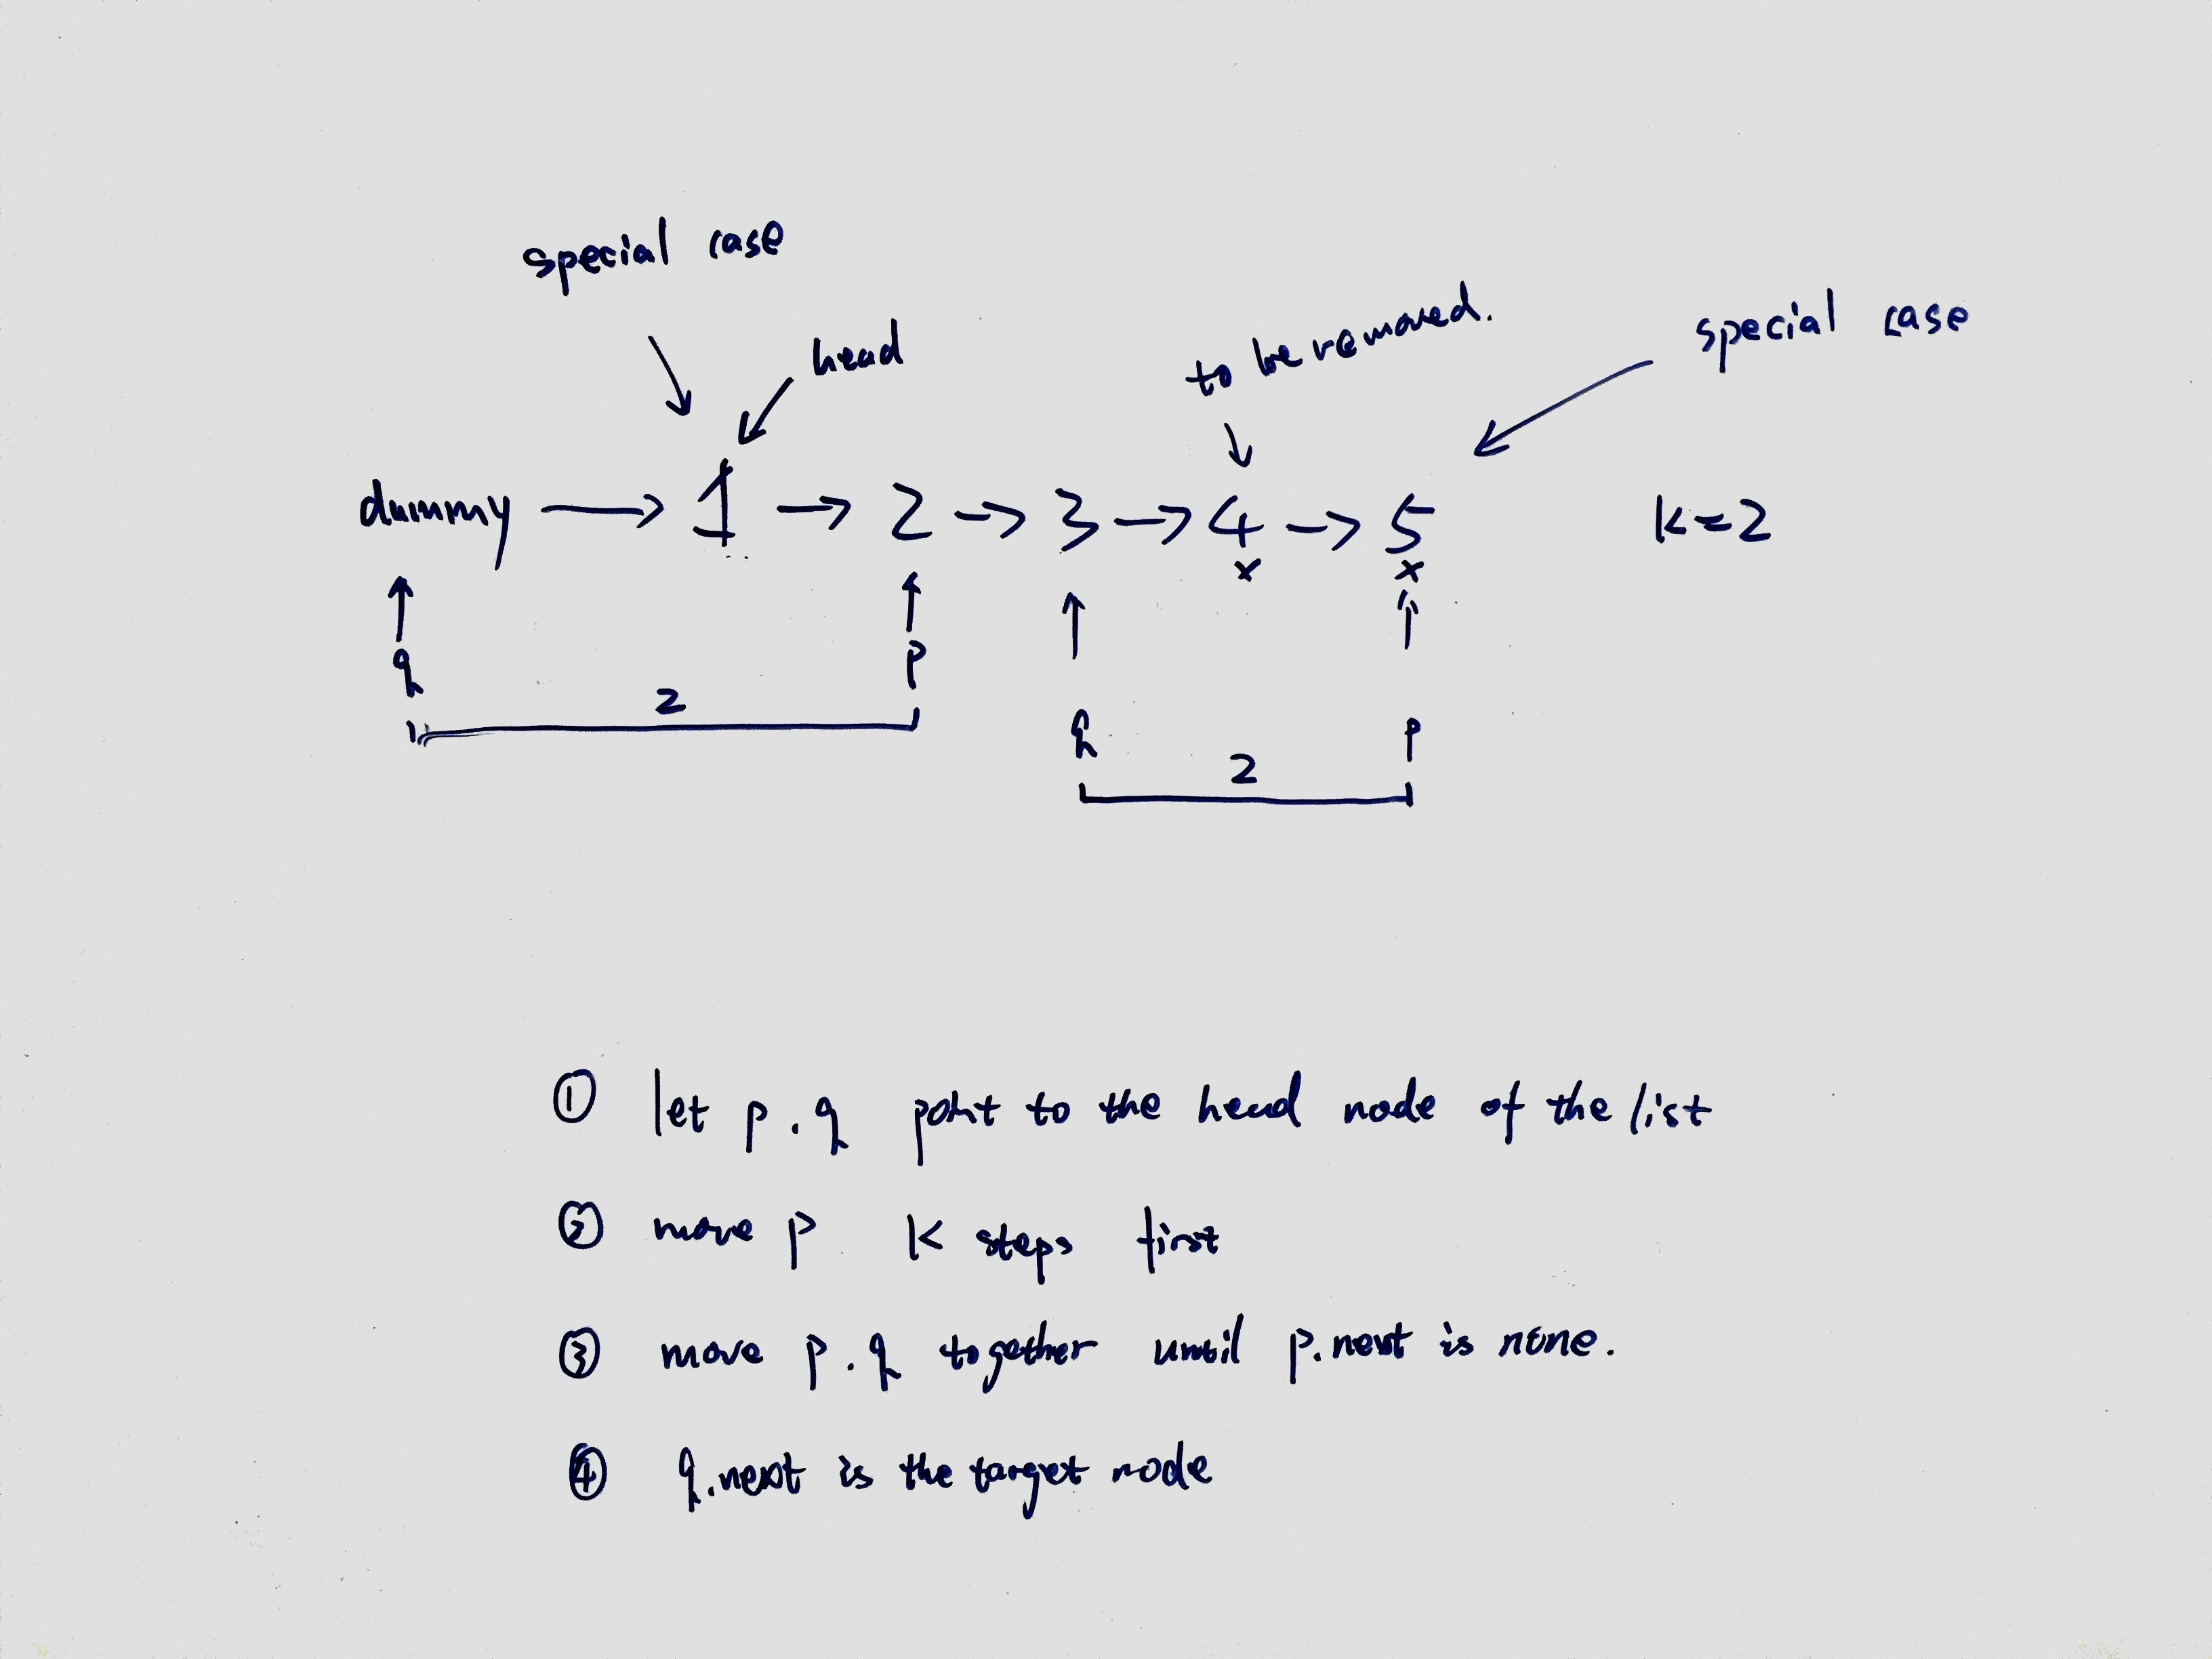
\includegraphics[width=\textwidth]{leetcode19.jpg}
    \centering \\
\end{figure}

\begin{lstlisting}[language=Python, caption=Problem19. Remove $N^{th}$ Node From End of List]

# Definition for singly-linked list.
# class ListNode(object):
#     def __init__(self, x):
#         self.val = x
#         self.next = None

class Solution(object):
    def removeNthFromEnd(self, head, n): # RT: O(n), space: O(1)
        """
        :type head: ListNode
        :type n: int
        :rtype: ListNode
        """
       def removeNthFromEnd(self, head, n):
        if head is None or (head.next is None and n == 1):
            return None

        dummy = ListNode(0)
        dummy.next = head
        fast = slow = dummy
        step = 0
        while step < n and fast:
            fast = fast.next
            step += 1

        if fast is None:
            return dummy.next

        while fast.next is not None:
            fast = fast.next
            slow = slow.next
        slow.next = slow.next.next
        return dummy.next
\end{lstlisting}



\subsubsection{leetcode 24. Swap Nodes in Pairs}
Given a linked list, swap every two adjacent nodes and return its head. For example, given 1->2->3->4, you should return the list as 2->1->4->3. \\

\noindent Your algorithm should use only \textbf{constant space}. You may \textbf{not modify the values} in the list, only nodes itself can be changed. \\

\begin{CJK*}{UTF8}{gbsn}
\noindent 解题思路:这道题使用快慢指针法,快慢指针的间距为2,即慢指针指向待交换的结点对儿的第一个结点的前驱结点,而快指针指向第二个结点。之所以这样设计指针的位置,是为了在交换结点的时候操作更方便。如果题目允许通过交换结点的值来完成结点交换的话,那么将慢指针指向第一个结点比较方便。但是本题要求的是不能通过值交换来达到结点交换的目的。\\
\end{CJK*}

\begin{lstlisting}[language=Python, caption=Problem24. Swap Nodes in Pairs]

# Definition for singly-linked list.
# class ListNode(object):
#     def __init__(self, x):
#         self.val = x
#         self.next = None

class Solution(object):
    def swapPairs_swapvalues(self, head):
        if head==None or head.next==None: return head
        p, q = head, head.next
        while True:
            p.val, q.val = q.val, p.val
            if q.next==None or q.next.next==None: break
            p = q.next
            q = p.next
        return head
    
    def swapPairs_swapnodes(self, head):
        """
        :type head: ListNode
        :rtype: ListNode
        """
        if head is None or head.next is None:
            return head

        dummy = ListNode(0)
        dummy.next = head
        slow = dummy
        fast = dummy.next

        while fast and fast.next:
            fast = fast.next

            # swap a node pair
            slow.next.next = fast.next
            fast.next = slow.next
            slow.next = fast

            # move fast and slow pointers to next position
            fast = fast.next.next
            slow = slow.next.next

        return dummy.next
\end{lstlisting}




\subsubsection{leetcode 25. Reverse Nodes in k-Group}
Given a linked list, reverse the nodes of a linked list $k$ at a time and return its modified list. If the number of nodes is not a multiple of k then left-out nodes in the end should remain as it is. You may not alter the values in the nodes, only nodes itself may be changed. \textbf{Only constant memory} is allowed. \\

\noindent For example, Given this linked list: 1->2->3->4->5
\begin{enumerate}
    \item For k = 2, you should return: 2->1->4->3->5
    \item For k = 3, you should return: 3->2->1->4->5 \\
\end{enumerate}

\begin{CJK*}{UTF8}{gbsn}
\noindent 解题思路:这道题实际是leetcode 24和leetcode92两道题的综合。这道题的解题过程包括两个主要部分:
\begin{itemize}
    \item 首先,确定反转区间。根据leetcode24的快慢指针设计思想,先移动快指针fast$n$次,让fast指向反转区间的尾结点,慢指针slow指向反转区间首结点的前驱结点。这样就确定了一个反转区间。在确定下一个反转区间的时候只需要将slow指针指向fast指针指向的结点,然后再按照上面的步骤移动fast就可以得到下一个反转区间了。
    \item 其次,反转包含$k$个结点的单链表。这个部分的算法设计可以参考leetcode92链表反转部分的算法。基本上,要使用三个指针pre, curr, next三个指针, pre和curr用于反转两个相邻结点之间的链,在反转完后pre指向curr,curr指向next
    ,然后移动next到下一个邻接结点。直到curr指向了反转区间的最后一个结点并完成了反转后,将slow所指向的结点的next指针指向的结点的next指针指向next指针当前指向的结点, 将slow指针所指向的结点的next指针指向curr指针当前指向的结点,这样就完成了反转过程。
\end{itemize}
\noindent另外,需要注意的一点是不足k长的部分无需翻转!
\end{CJK*}

\begin{figure}[h]
    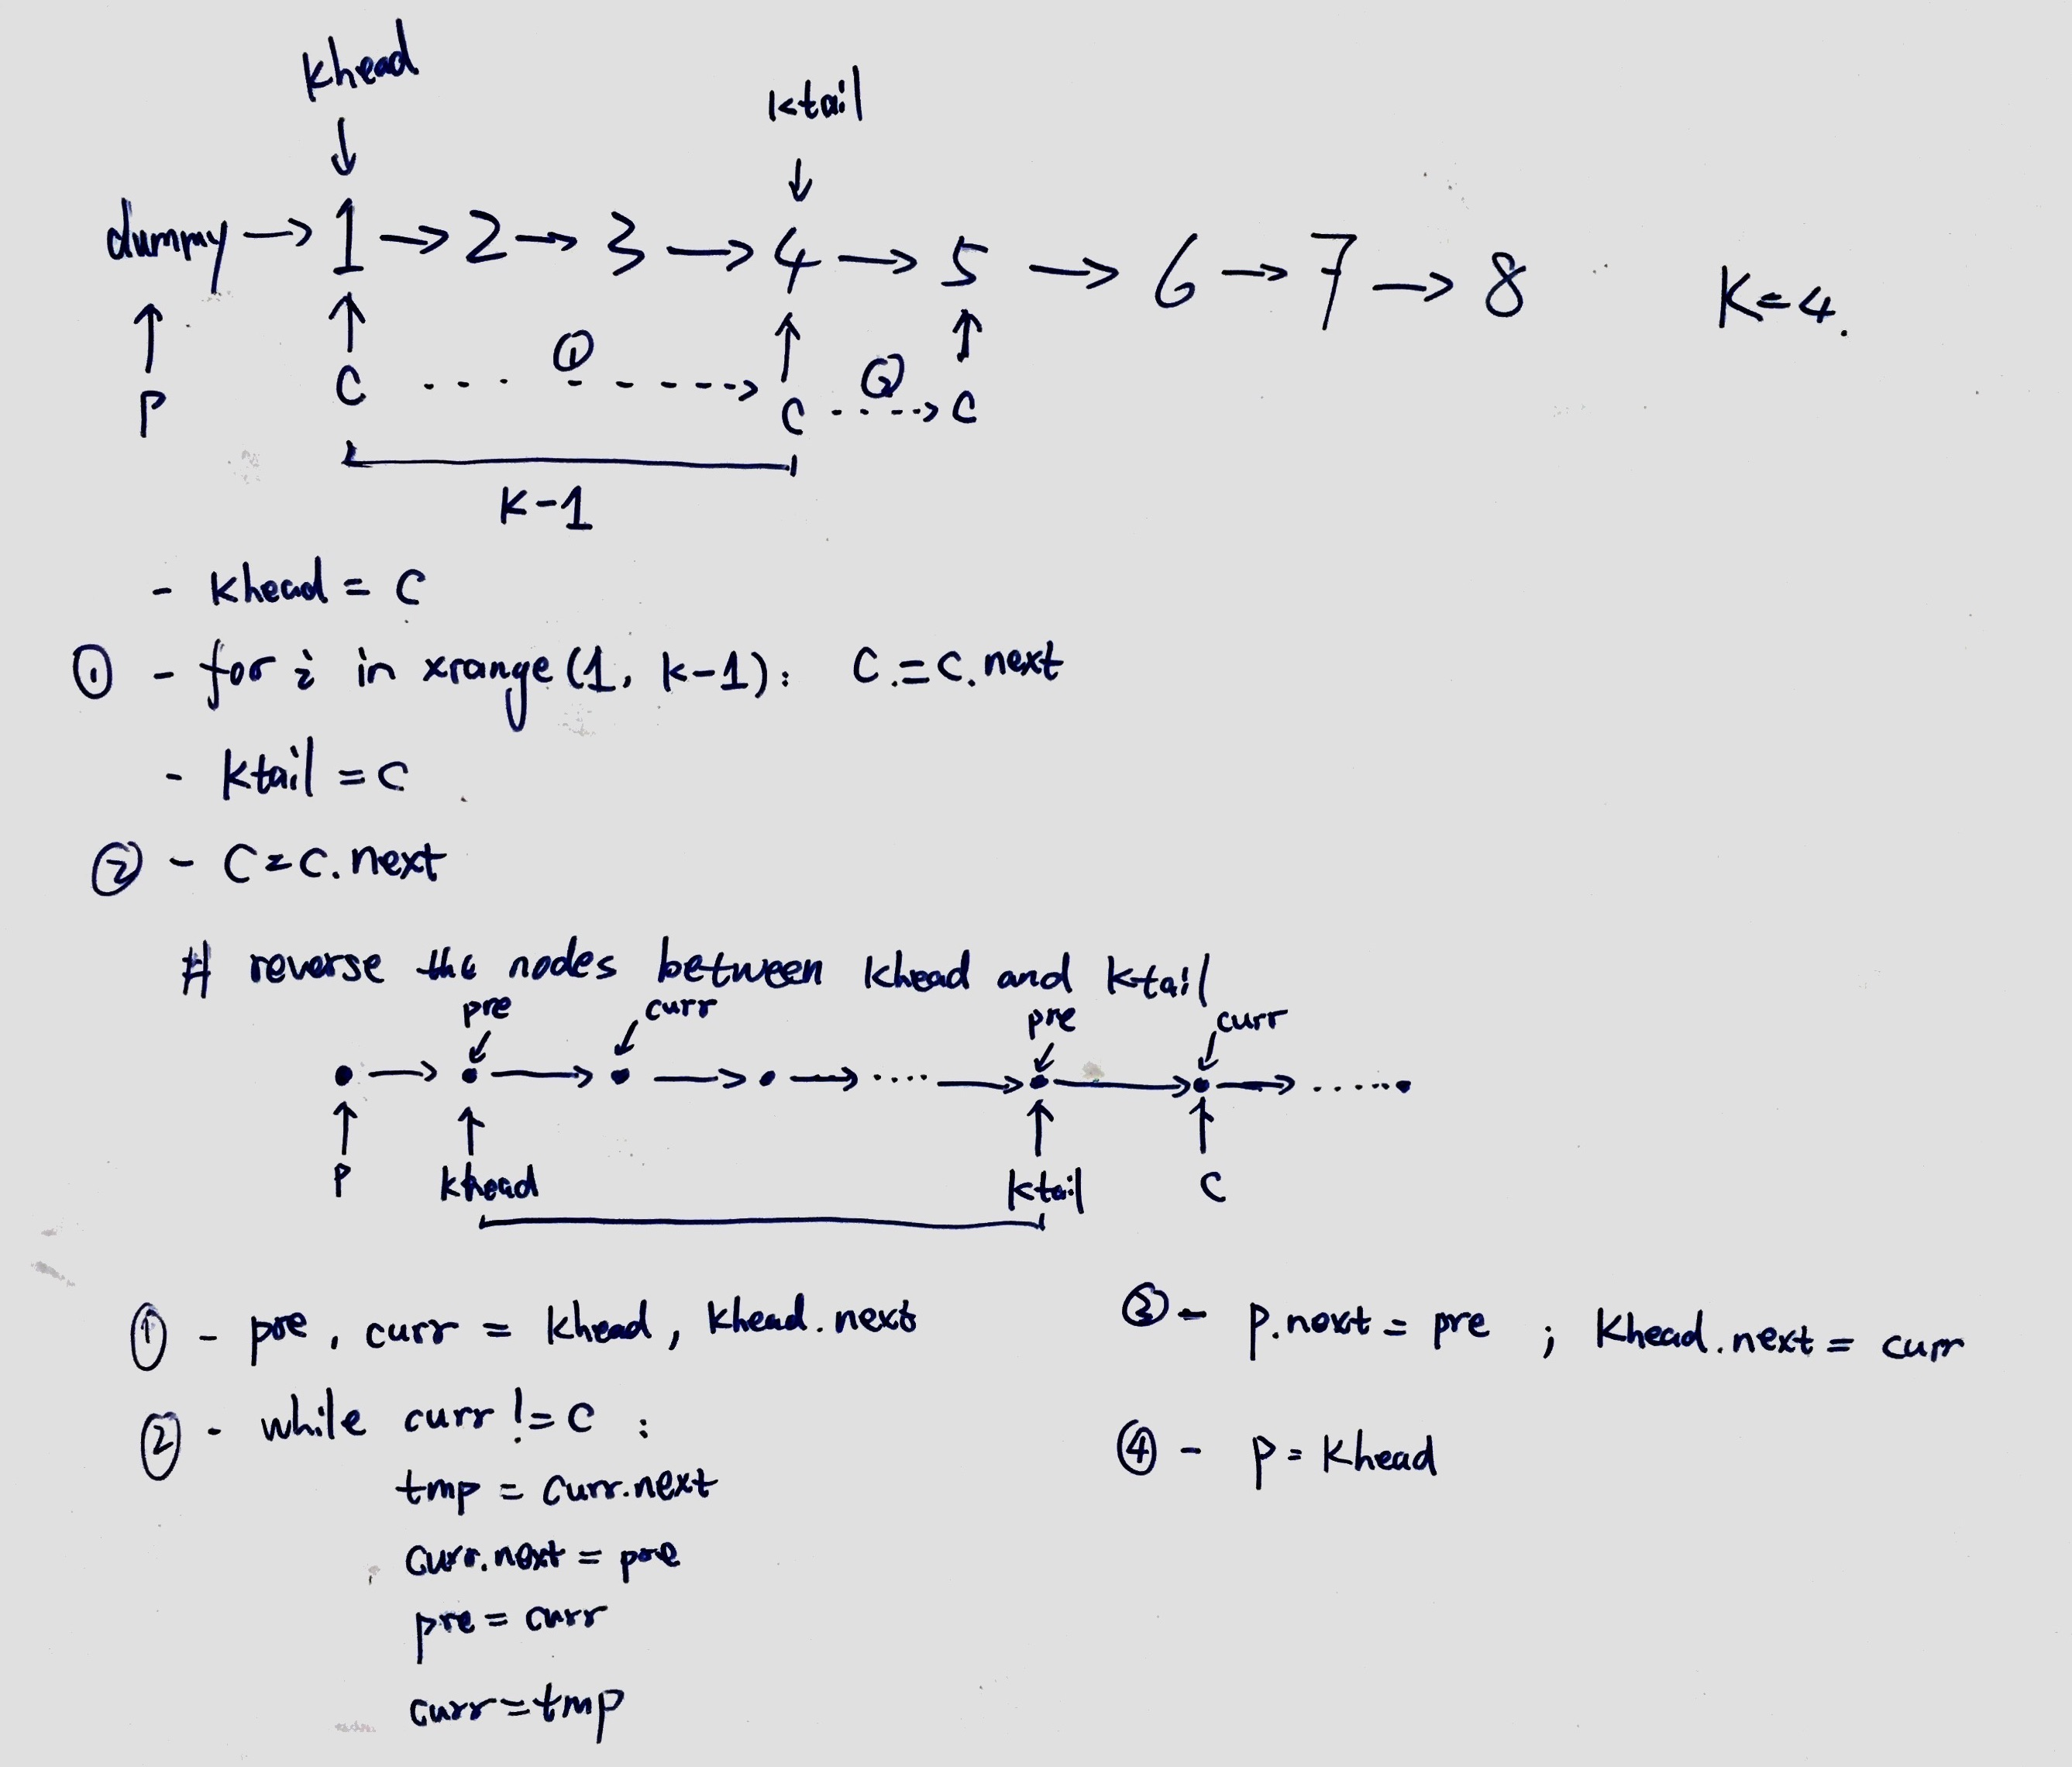
\includegraphics[width=\textwidth]{leetcode25.jpg}
    \centering \\
\end{figure}

\begin{lstlisting}[language=Python, caption=Problem25. Reverse Nodes in k-Group]

# Definition for singly-linked list.
# class ListNode(object):
#     def __init__(self, x):
#         self.val = x
#         self.next = None

class Solution(object):
    def reverseKGroup(self, head, k):
        """
        :type head: ListNode
        :type k: int
        :rtype: ListNode
        """
        if head is None or k == 1:
            return head

        dummy = ListNode(0)
        dummy.next = head
        slow = dummy
        fast = dummy.next
        while fast:
            # fix a k-size range to reverse
            step = 0
            while step < k - 1 and fast:
                fast = fast.next
                step += 1

            if fast is None: return dummy.next

            # reverse the node in k-group
            headptr, pre, curr, nextptr = slow.next, slow.next, slow.next.next, slow.next.next.next
            while pre != fast:
                curr.next = pre
                pre = curr
                curr = nextptr
                if nextptr is not None:
                    nextptr = nextptr.next
            slow.next.next = curr
            slow.next = pre

            # move slow and fast points for next round
            slow = headptr
            fast = curr

        return dummy.next
\end{lstlisting}








\subsubsection{leetcode 138. Copy List with Random Pointer}
A linked list is given such that each node contains an additional random pointer which could point to any node in the list or null. Return a deep copy of the list. \\

\begin{CJK*}{UTF8}{gbsn}
\noindent 解题思路:这题的难点在于如何处理random指针。方法是为链表中的每一个结点创建一个副本,并将副本插入到每一个原始结点的后面;遍历更新后的链表,让p指向每一个原始结点,使得p.next.random = p.random.next。完成所有副本结点的random指针赋值后,再分离出深度复制后的链表。\\
\end{CJK*}

\begin{lstlisting}[language=Python, caption=Problem138. Copy List with Random Pointer]

# Definition for singly-linked list with a random pointer.
# class RandomListNode(object):
#     def __init__(self, x):
#         self.label = x
#         self.next = None
#         self.random = None

class Solution(object):
    def copyRandomList(self, head): # RT: O(n)
        """
        :type head: RandomListNode
        :rtype: RandomListNode
        """
        if head==None: return head
        
        # copy every existed node in the original
        # list and insert the copy node into the list
        # just next to the original node.
        # before: 1->2->3->4
        # after:  1->1->2->2->3->4->4
        p = head
        while p!=None:
            node = RandomListNode(p.label)
            tmp = p.next
            node.next = tmp
            p.next = node
            p = node.next
        
        # deal with the random pointers
        p = head
        while p!=None:
            if p.random!=None:
                p.next.random = p.random.next
            p = p.next.next
        
        # separate the copy list from the 
        # the hybrid list, and recover the
        # original list
        dummy = RandomListNode(0)
        dummy.next = head.next
        q = dummy
        p = head
        while p!=None:
            q.next = p.next
            p.next = p.next.next
            q = q.next
            p = p.next
            
        return dummy.next
\end{lstlisting}

\begin{figure}[h]
    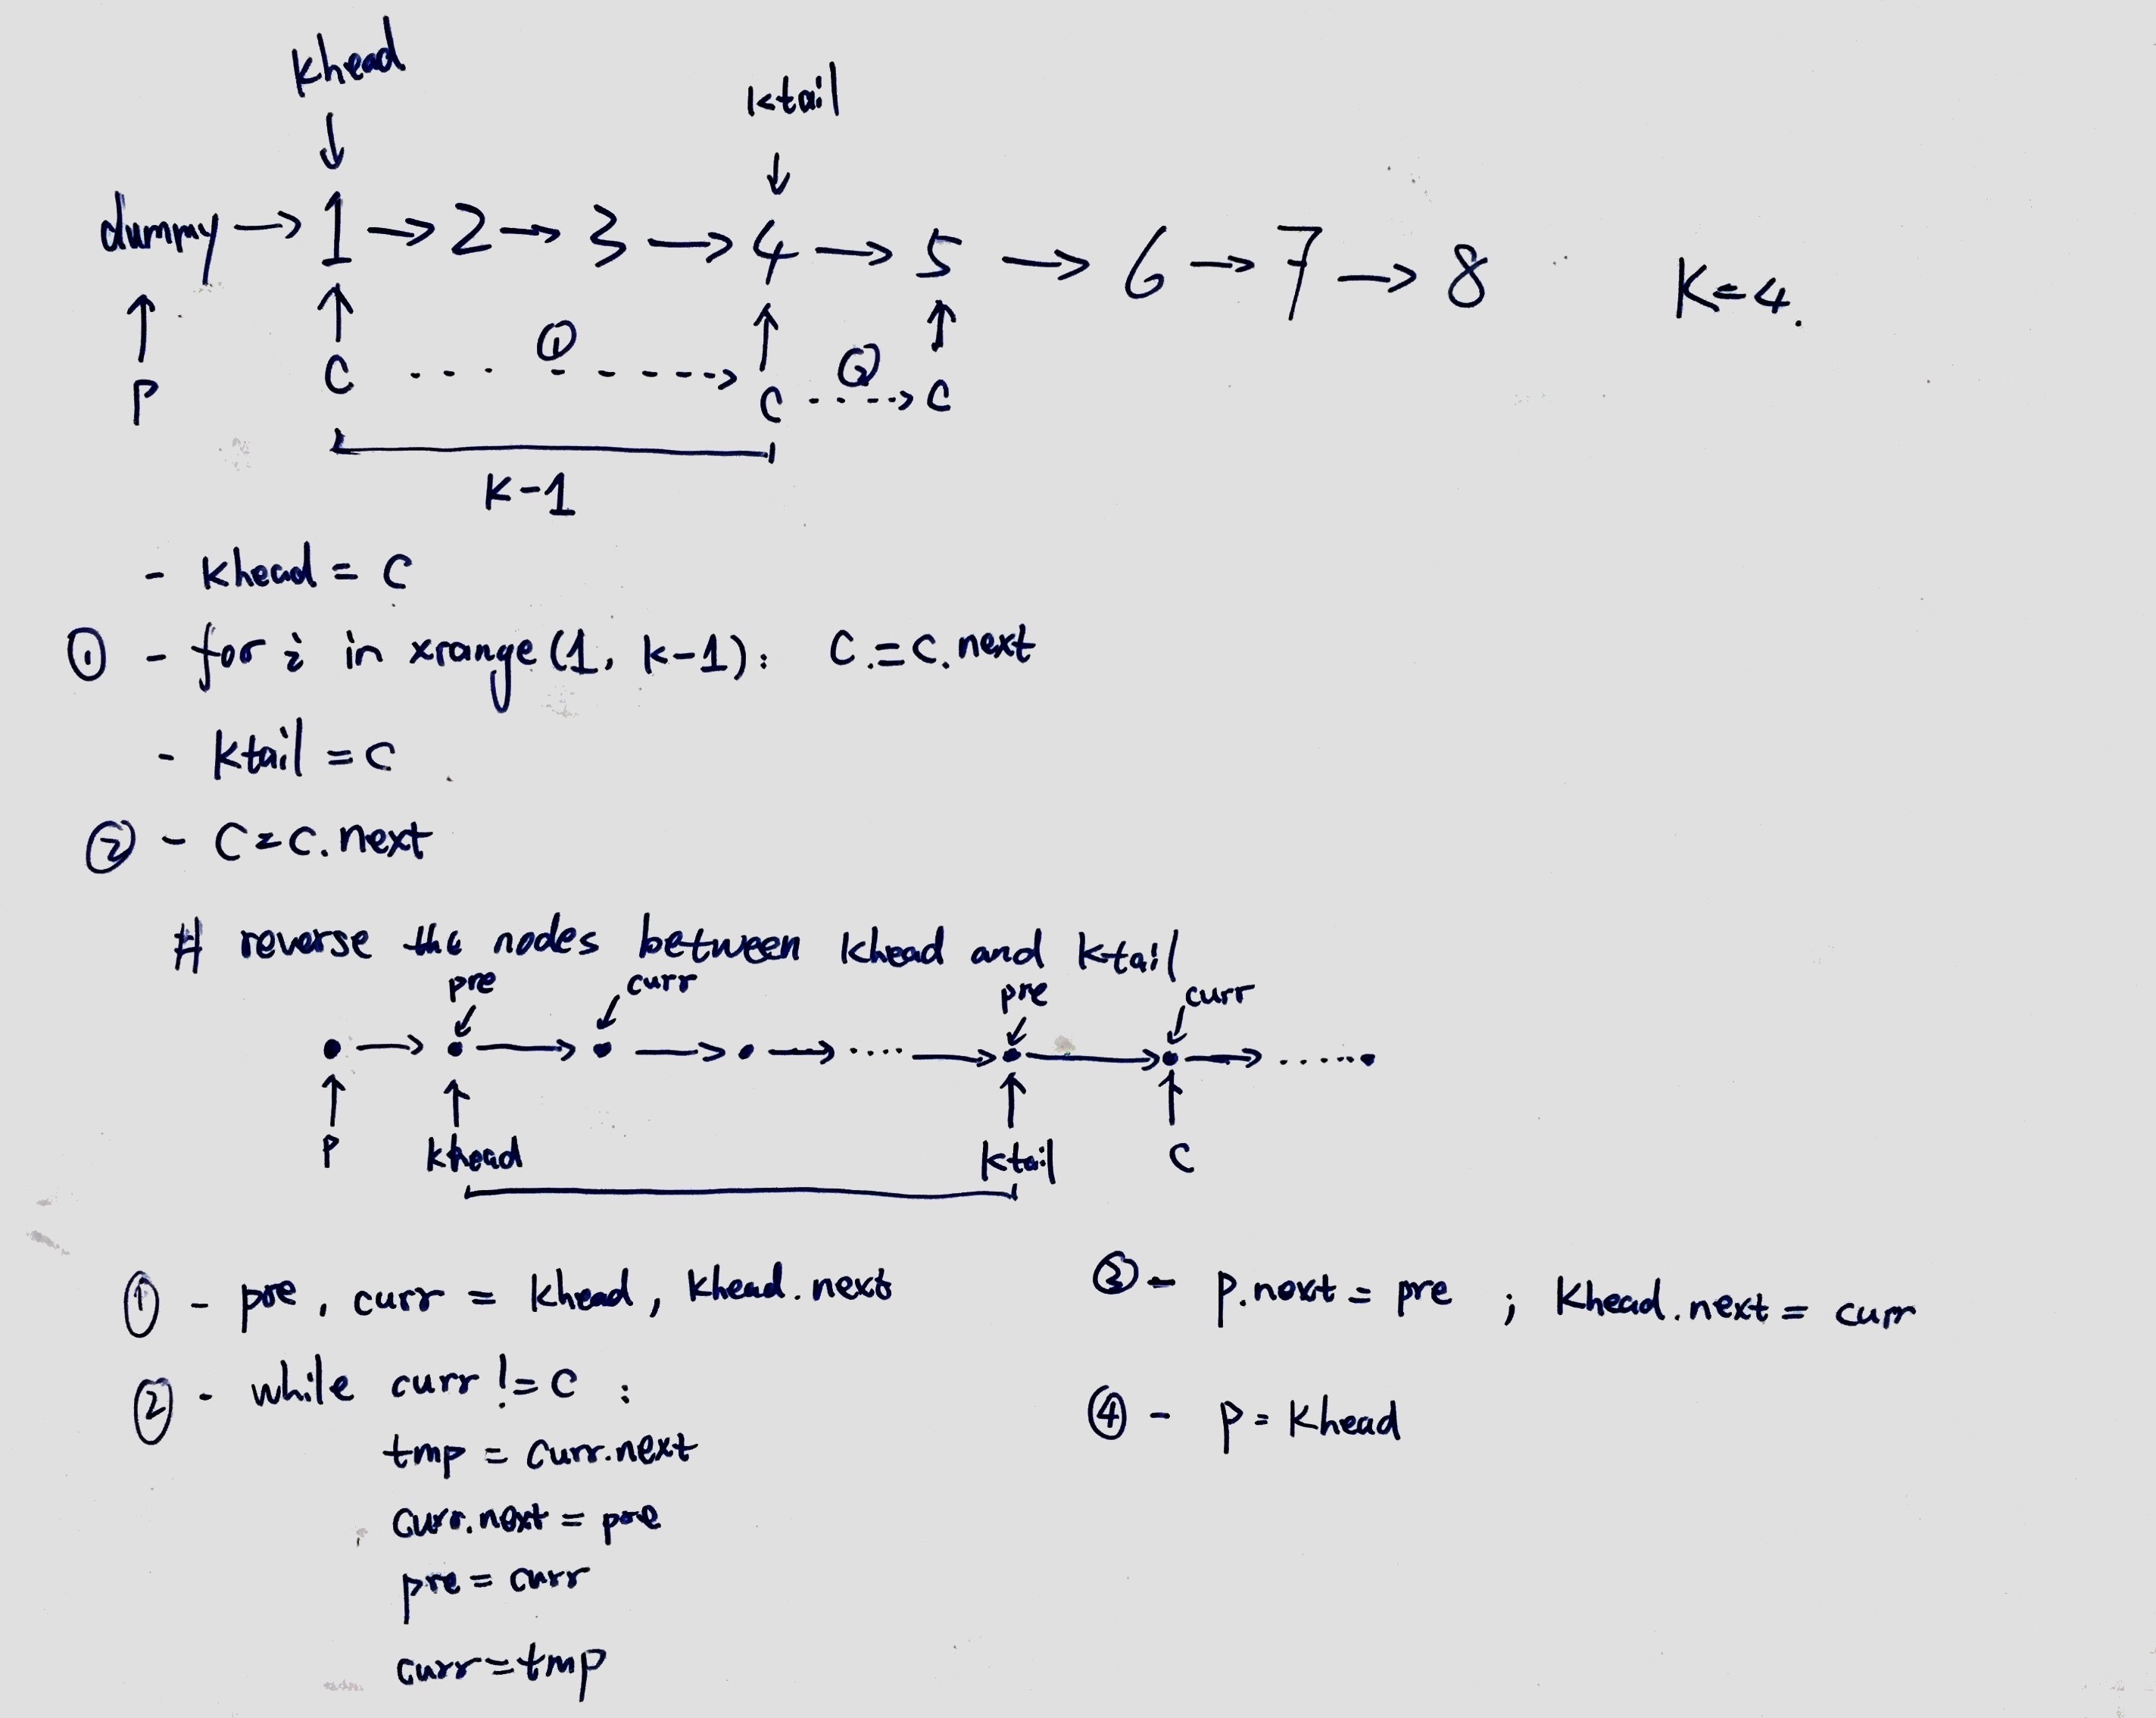
\includegraphics[width=\textwidth]{leetcode138.jpg}
    \centering \\
\end{figure}




\subsubsection{leetcode 141. Linked List Cycle}
Given a linked list, determine if it has a cycle in it. Follow up: Can you solve it without using extra space? \\

\begin{CJK*}{UTF8}{gbsn}
\noindent 解题思路:使用快慢指针的方法:快指针fast一次走两步,慢指针slow一次走一步,如果两个指针最后相遇,那么说明当前的链表有环。注意这道题的原理需要清楚地知道。\\
\end{CJK*}

\begin{lstlisting}[language=Python, caption=Problem141. Linked List Cycle]

# Definition for singly-linked list.
# class ListNode(object):
#     def __init__(self, x):
#         self.val = x
#         self.next = None

class Solution(object):
    def hasCycle(self, head):
        """
        :type head: ListNode
        :rtype: bool
        """
        if head==None or head.next==None: return False
        slow = fast = head
        while fast.next and fast.next.next:
            fast = fast.next.next
            slow = slow.next
            if fast == slow: return True
        return False
\end{lstlisting}


\subsubsection{leetcode 142. Linked List Cycle II}
Given a linked list, return the node where the cycle begins. If there is no cycle, return null. Note: Do not modify the linked list. \\

\noindent Follow up: Can you solve it without using extra space? \\

\begin{CJK*}{UTF8}{gbsn}
\noindent 解题思路:这道题是在leetcode141的基础上,增加了难度,需要在环存在的情况下,确定环的入口点。使用快慢指针的方法确定是否有环(参考leetcode141的说明)。在fast和slow两个指针相遇后,再使用一个单步指针从链表的头结点开始,同时移动单步指针和slow指针,当这两个指针相遇时,即为环的入口点。需要清楚原理。\\
\end{CJK*}

\begin{lstlisting}[language=Python, caption=Problem142. Linked List Cycle II]

# Definition for singly-linked list.
# class ListNode(object):
#     def __init__(self, x):
#         self.val = x
#         self.next = None

class Solution(object):
    def detectCycle(self, head):
        """
        :type head: ListNode
        :rtype: ListNode
        """
        if head==None or head.next==None:
            return None
        
        # First, check if a cycle exists in
        # the list.
        p = head.next.next
        q = head.next
        while p!=None and p!=q:
            if p.next!=None and p.next!=None:
                p = p.next.next
                q = q.next
            else:
                return None
        
        if p==None: return None
        # Second, when p==q, the cycle exists,
        # and from the node where p meets q, move
        # pointer r from the beginning of the list
        # with the same step as q. when r,q meet 
        # at some node, the node is just the result.
        r = head
        while r!=q:
            r = r.next
            q = q.next
        
        return r
\end{lstlisting}



\subsubsection{leetcode 143. Reorder List}
Given a singly linked list $L: L_0\to L_1\to \dots \to L_{n-1} \to L_n,$
reorder it to: $L_0 \to L_n \to L_1 \to L_{n-1} \to L_2 \to L_{n-2} \to \dots$. You must do this in-place without altering the nodes' values. For example, given {1,2,3,4}, reorder it to {1,4,2,3}. \\

\begin{CJK*}{UTF8}{gbsn}
\noindent 解题思路:参见示例图,题目的解法分为三个部分:
\begin{itemize}
    \item 首先,使用快慢指针法找到分割点:快指针一次走两步,慢指针一次走一步,从伪头结点dummy开始。在分割点之前(包括分割点)为第一部分,分割点之后为第二部分。考虑到原链表中结点的数目可能为奇数也可能为偶数,所以第二部分所含结点的个数不多于第一部分。如示例图所示。
    \item 其次,反转第二部分的链表结点:参考leetcode92的算法。
    \item 最后,合并第一、二两部分的结点。合并的原则是每一轮在第一、二部分各取一个结点加入,直到第二个部分的所有结点都已经插入。最后,如果第一部分还有结点未插入,那么插入剩余结点。
\end{itemize}
\end{CJK*}


\begin{lstlisting}[language=Python, caption=Problem143. Reorder List]

# Definition for singly-linked list.
# class ListNode(object):
#     def __init__(self, x):
#         self.val = x
#         self.next = None

class Solution(object):
    def reorderList(self, head):
        """
        :type head: ListNode
        :rtype: void Do not return anything, modify head in-place instead.
        """
        if head==None or head.next==None: return
        dummy = ListNode(0)
        dummy.next = head
        # divide the original list into two parts
        slow = fast = dummy
        while fast.next and fast.next.next:
            fast = fast.next.next
            slow = slow.next
        if fast.next==None: # has even nodes
            head2 = slow.next
            tail1 = slow
        elif fast.next.next==None: # has odd nodes
            head2 = slow.next.next
            tail1 = slow.next
        tail1.next = None
        
        # reverse the second half part
        pre, curr = head2, head2.next
        while curr:
            tmp = curr.next
            curr.next = pre
            pre = curr
            curr = tmp
        head2.next = None
        head2 = pre
        
        # merge two parts
        p = head
        while head2:
            tmp = head2.next
            head2.next = p.next
            p.next = head2
            p = head2.next
            head2 = tmp
\end{lstlisting}

\begin{figure}[h]
    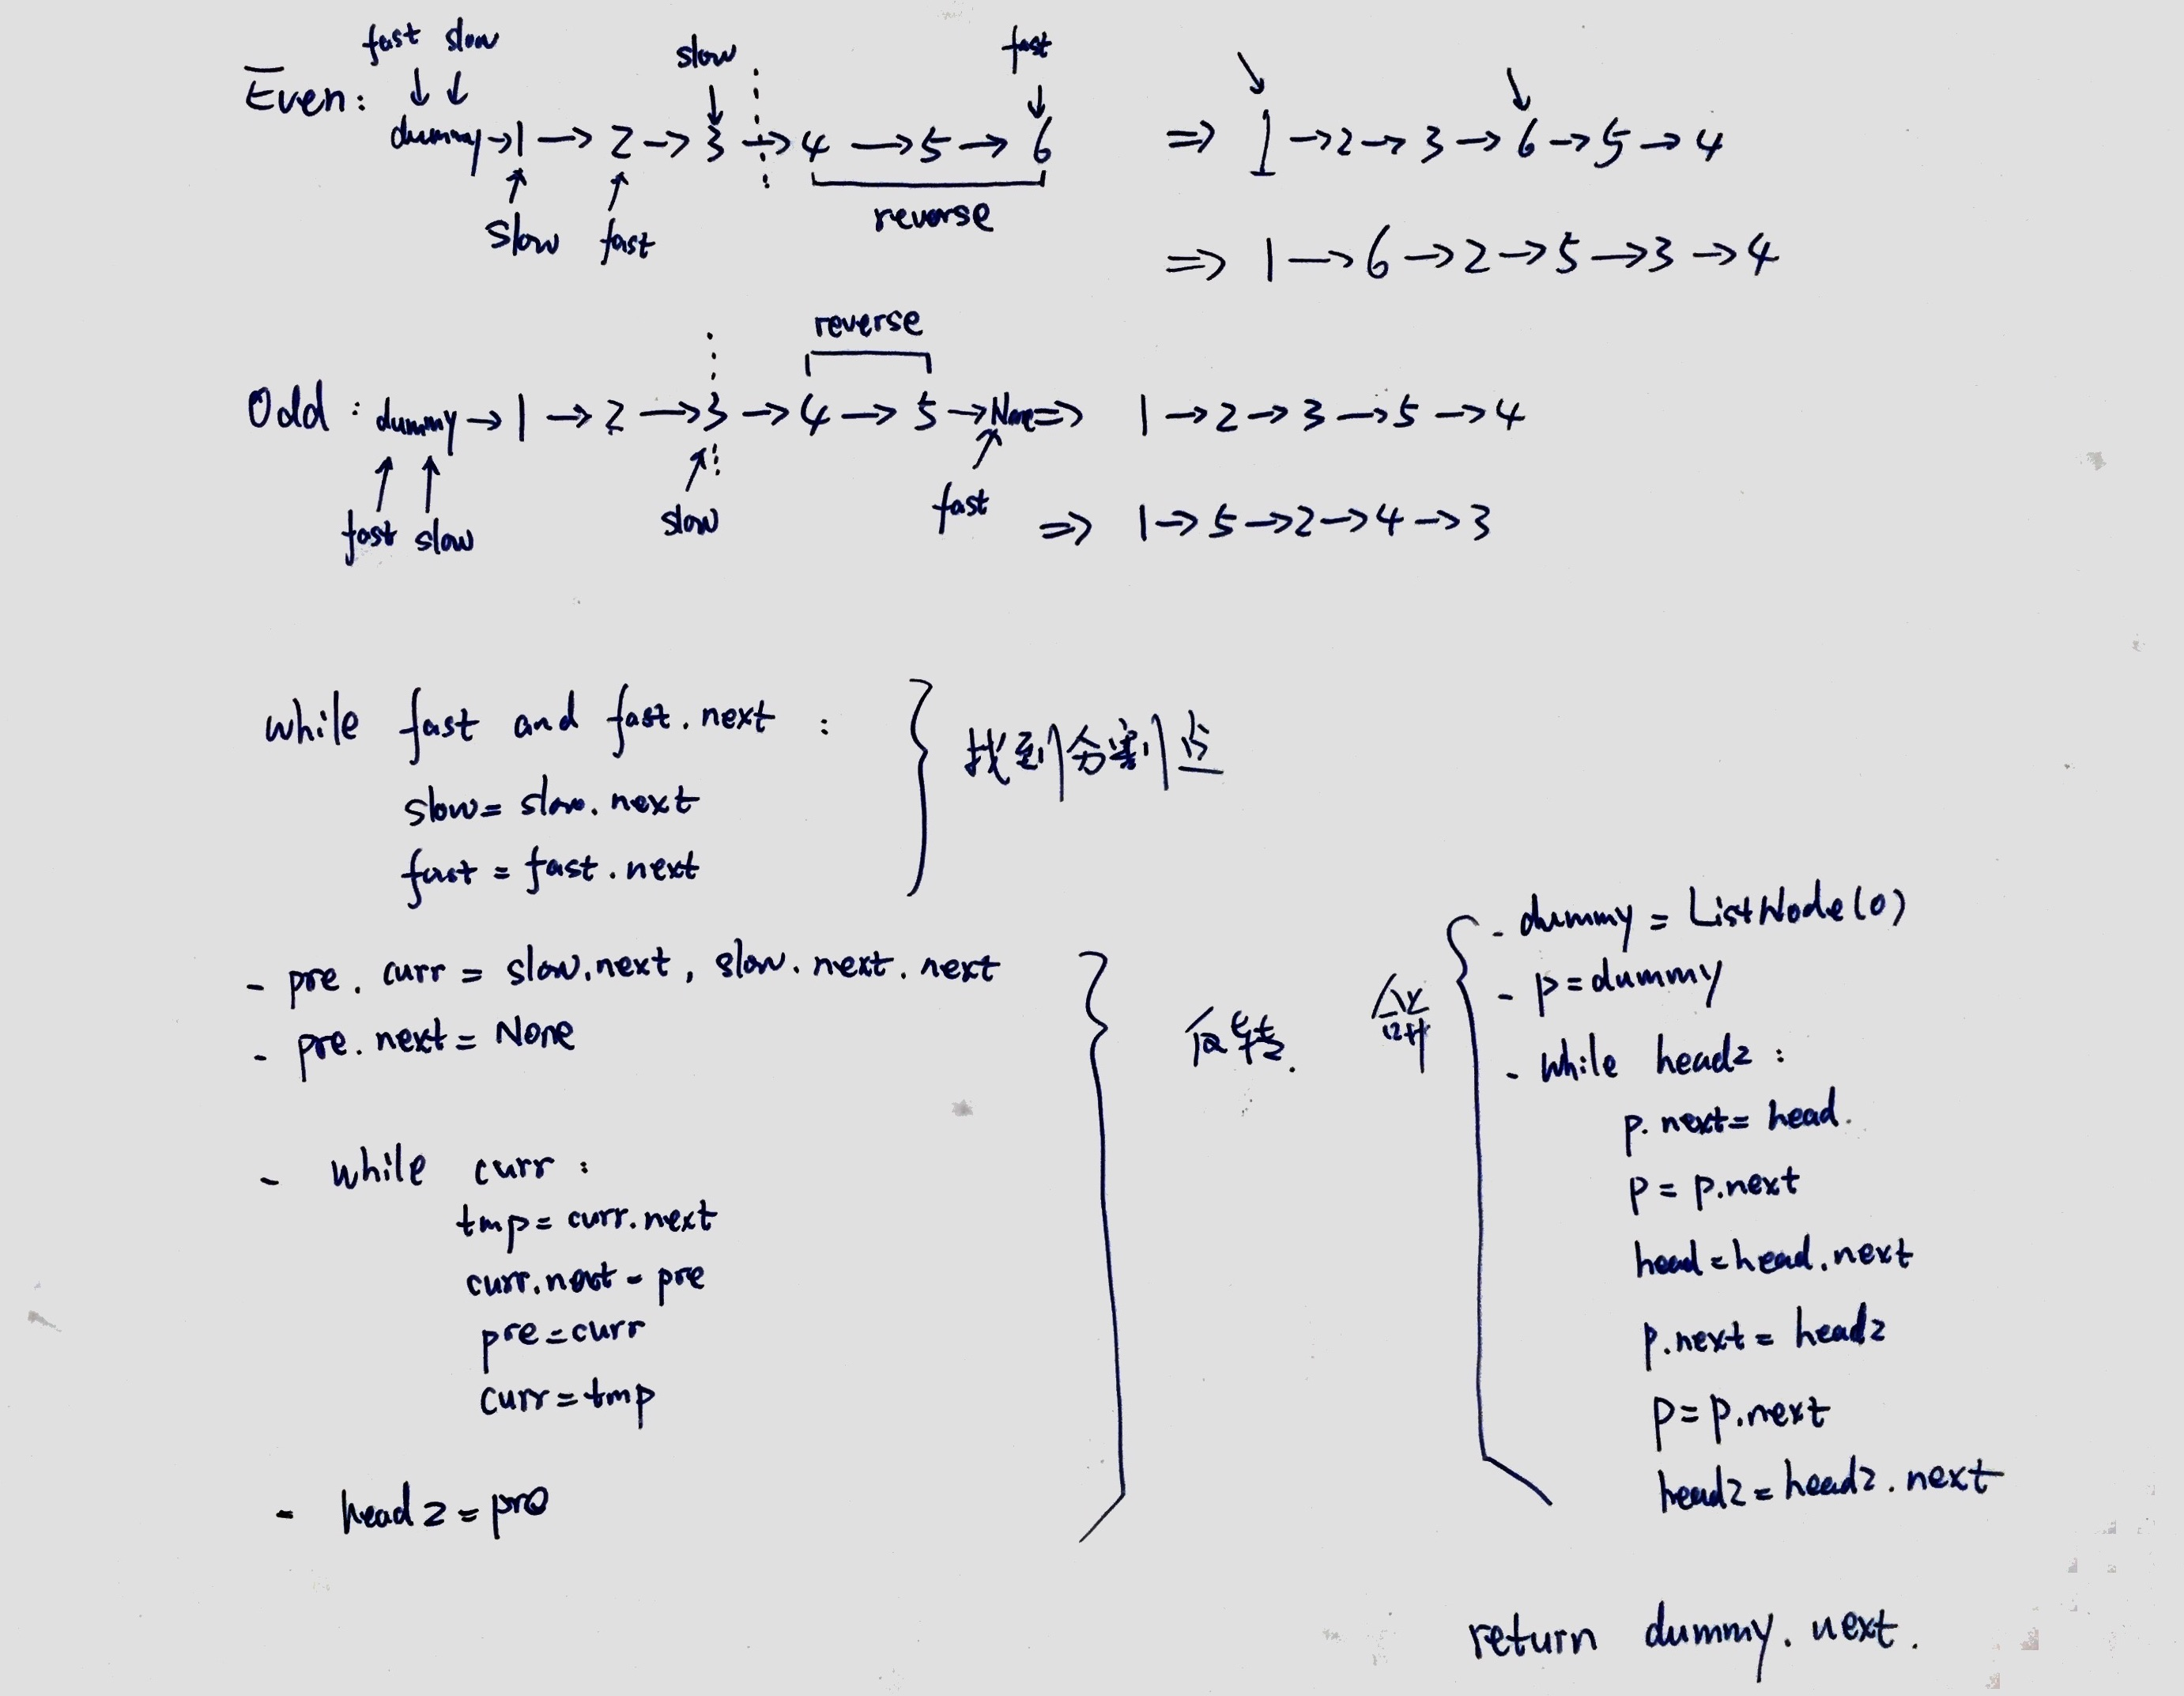
\includegraphics[width=\textwidth]{leetcode143.jpg}
    \centering \\
\end{figure}









%%%%%%%%%%%%%%%%%%%%%%%%%%%%%%%%%%%%%%%%%%%%%%%%%%%%%%
%%%%%%%%%%%%%%%%% 字符串 %%%%%%%%%%%%%%%%%%%%%%%%%%%%%
%%%%%%%%%%%%%%%%%%%%%%%%%%%%%%%%%%%%%%%%%%%%%%%%%%%%%%
\section{Strings}

\subsection{Summary}
\begin{CJK*}{UTF8}{gbsn}
\noindent 总结:与字符串相关的算法题目
\begin{enumerate}
    \item 字符串匹配类问题:目前流行的字符串匹配算法有以下七种:
        \begin{itemize}
            \item Brute-force search(暴力法)$O(m \times n)$
            \item KMP算法$O(m+n)$
            \item $Z$算法$O(m+n)$
            \item Robin-Karp算法: It uses hashing to find any one of a set of pattern strings in a text. Its average and best case running time is $O(n+m)$ in space $O(m)$, but its worst-case time is $O(m \times n)$.
            \item Boyer-Moore算法
            \item Aho-Corasick算法: worst-time complexity $O(m+n)$ in space $O(m)$. It is a kind of dictionary-matching algorithm that locates elements of a finite set of strings (the "dictionary") within an input text. It matches all strings simultaneously.
            \item 有限状态机
        \end{itemize}
    
    \item Palindrome类问题
        \begin{itemize}
            \item DP-I算法: $O(n^2)$ time in $O(n^2)$ space
            \item DP-II算法: $O(n^2)$ time in $O(1)$ space
            \item Manacher's algorithm: $O(n)$ time in $O(n)$ space
        \end{itemize}
\end{enumerate}
\end{CJK*}


\subsection{leetcode 65. Valid Number}
Validate if a given string is numeric. Some examples:
\begin{enumerate}
    \item "0" => true
    \item "0.1" => true
    \item "abc" => false
    \item "1a" => false
    \item "2e10" => true
\end{enumerate}

\noindent Note: It is intended for the problem statement to be ambiguous. You should gather all requirements up front before implementing one.

\begin{CJK*}{UTF8}{gbsn}
\noindent 解题思路:建立状态机,如下图所示。这个题有9种状态:
\begin{itemize}
    \item 0: 初始无输入或者只有space的状态
    \item 1: 输入了数字之后的状态
    \item 2: 前面无数字,只输入了dot的状态
    \item 3: 输入了符号状态
    \item 4: 前面有数字和有dot的状态
    \item 5: 'e' or 'E'输入后的状态
    \item 6: 输入e之后输入Sign的状态
    \item 7: 输入e后输入数字的状态
    \item 8: 前面有有效数输入之后,输入space的状态
\end{itemize}
\end{CJK*}

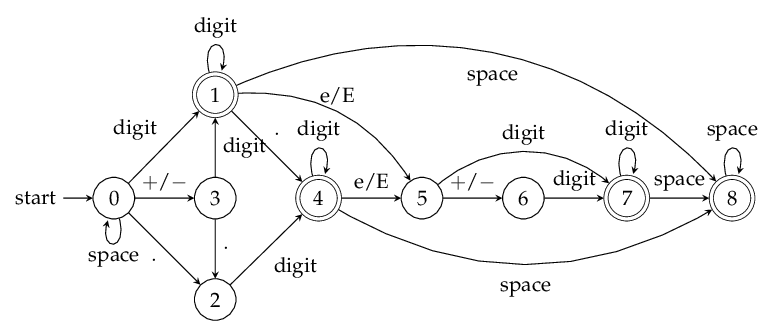
\includegraphics[width=\textwidth]{state} \\
\begin{lstlisting}[language=Python, caption=Problem65. Valid Number]

class Solution(object):
    def isNumber(self, s):
        """
        :type s: str
        :rtype: bool
        """
        INVALID=0; SPACE=1; SIGN=2; DIGIT=3; DOT=4; EXPONENT=5;
        #0invalid,1space,2sign,3digit,4dot,5exponent,6num_inputs
        transitionTable=[
            [-1,  0,  3,  1,  2, -1],    #0 no input or just spaces 
            [-1,  8, -1,  1,  4,  5],    #1 input is digits 
            [-1, -1, -1,  4, -1, -1],    #2 no digits in front just Dot 
            [-1, -1, -1,  1,  2, -1],    #3 sign 
            [-1,  8, -1,  4, -1,  5],    #4 digits and dot in front 
            [-1, -1,  6,  7, -1, -1],    #5 input 'e' or 'E' 
            [-1, -1, -1,  7, -1, -1],    #6 after 'e' input sign 
            [-1,  8, -1,  7, -1, -1],    #7 after 'e' input digits 
            [-1,  8, -1, -1, -1, -1]]    #8 after valid input input space
        state=0; i=0
        while i<len(s):
            inputtype = INVALID
            if s[i]==' ': inputtype=SPACE
            elif s[i]=='-' or s[i]=='+': inputtype=SIGN
            elif s[i] in '0123456789': inputtype=DIGIT
            elif s[i]=='.': inputtype=DOT
            elif s[i]=='e' or s[i]=='E': inputtype=EXPONENT
            
            state=transitionTable[state][inputtype]
            if state==-1: return False
            else: i+=1
        return state == 1 or state == 4 or state == 7 or state == 8
\end{lstlisting}


\subsection{leetcode 125. Valid Palindrome}
Given a string, determine if it is a palindrome, considering \textbf{only alphanumeric} characters and \textbf{ignoring cases}. For example,
\begin{itemize}
    \item "A man, a plan, a canal: Panama" is a palindrome.
    \item "race a car" is not a palindrome.
\end{itemize}

\noindent Note: Have you consider that the string might be empty? This is a good question to ask during an interview. For the purpose of this problem, we define empty string as valid palindrome.\\

\begin{CJK*}{UTF8}{gbsn}
\noindent 解题思路:这道题的算法设计并不难,而且也是面试中常常会被问及的问题。但是,这道题的考查点是在设计算法之前,是否问清楚了题目中的一些潜在的(或者说没有在题目中明确说明的)需求。比如,目标字符串到底是什么样子的,题目下面有提示说字符串为空时的情形。题目也给出只考虑英文字符和数字,也暗示字符串本身可能包括其他字符,那么就需要在验证palindrome属性之前,对字符串先行处理一下;去掉不符合要求的字符以后才能进行比较。这条信息在题目中已经给出,但是在面试的时候,面试官通常并不会像题目中那样给出这些明确的或者暗示性的信息,因此要特别注意所有题目中给出的各种前提条件。在面试过程中,如果碰到相似的题目时,必须在设计算法前,首先确定题目的前提条件是否一致。如果前提条件是不一样的,那么即使做过类似的题目,设计出来的算法也可能有很大的不同。即使是完全相同的题目,如果在没有询问面试官确定这些前提条件的话,即使设计出了正确的算法,也是失败的过程。\\
\end{CJK*}

\begin{lstlisting}[language=Python, caption=Problem125. Valid Palindrome]

class Solution(object):
    def isPalindrome1(self, s): # RT: O(n), Space: O(n)
        """
        :type s: str
        :rtype: bool
        """
        if s==None: return False
        if len(s)<=1: return True
        
        # only extract alphanumeric characters
        str=[c for c in s.lower() if 97<=ord(c)<=122 or 48<=ord(c)<=57]
        return str==str[::-1]
\end{lstlisting}


\subsection{leetcode 28. Implement strStr()}
Implement strStr(). Returns the index of the first occurrence of needle in haystack, or -1 if needle is not part of haystack. \\

\begin{CJK*}{UTF8}{gbsn}
\noindent 解题思路:这道题实际上就是在文本中搜索指定的字符串。至少有四种解决方法方法。为了描述方便,假设heystack就是文本text,长度为$m$,needle就是pattern,即要搜索的字符串,长度为$n$。解决方法如下:
\begin{enumerate}
    \item 暴力破解法:这种方法就是先在text中找到与pattern的首字符匹配的字符位置;然后在依次验证后面相应的字符是否每一个都匹配。如果匹配,就返回首字母在text中的索引;如果出现不匹配的字符,就重新开始搜索和匹配过程。这种方法的时间复杂度是$O(m \times n)$,空间复杂度是$O(1)$。
    
    \item KMP算法:最著名的字符串匹配算法,算法时间复杂度为$O(m+n)$。该算法分为两个阶段(参考下面的示例图一):
        \begin{itemize}
            \item 第一阶段的任务是遍历pattern建立T表。这个T表的作用是在第二阶段的匹配过程中,如果text[i]$\neq$pattern[j],那么就验证pattern[T[j-1]]与text[i]是否匹配。完成这个任务的时间复杂度是$O(n)$。
            \item 第二阶段的任务就是在text中搜索pattern。在不匹配的情况发生时,只需要利用第一阶段生成的T表,在$O(1)$的时间内确定应该回到pattern的哪一个字符再进行匹配比较。因为遍历完text即完成匹配搜索,所以这个阶段的时间复杂度是$O(m)$。
        \end{itemize}
    
    \item $Z-$算法:这个算法是将pattern与text连接成一个字符串,其中pattern是这个新字符串的前缀子串。然后,然后使用一个$m+n$长的数组$Z$用于存储计算过程中的中间值。Z[i]表示以字符串的第$i$个字符为起点所构成的最长前缀字符串的长度值。存储参考下面的示例图二中的描述和演算过程。这个算法的时间复杂度是$O(m+n)$,空间复杂度是$O(m+n)$。
    
    \item Rabin-Karp算法:RK算法的时间复杂度是$O(m \times n)$,空间复杂度是$O(1)$。这个算法最适合在一个text中搜索多个pattern的情形。另外,这个算法的特点是利用哈希函数来确定潜在的匹配项,然后再通过精确匹配的进行验证。哈希函数和演算的细节参考示例图三。
    \iffalse
    \item Boyer-Moore算法:这种算法适用于pattern的长度相对于text的长度比较短的情况。另外,BM算法需要预处理pattern,在这个过程中根据bad character rule和good suffix rule建立两组不同的table。而字符串匹配的过程每次都是从pattern的尾部开始;在不匹配情况发生时,pattern向前移动的距离是由max(1, bad character rule, good suffix rule)决定的。
    \fi
\end{enumerate}

\noindent 这道题仅要求判断是否存在匹配。可以进一步扩展为输出所有匹配在text中的起始位置索引。
\end{CJK*}

\begin{figure}[h]
    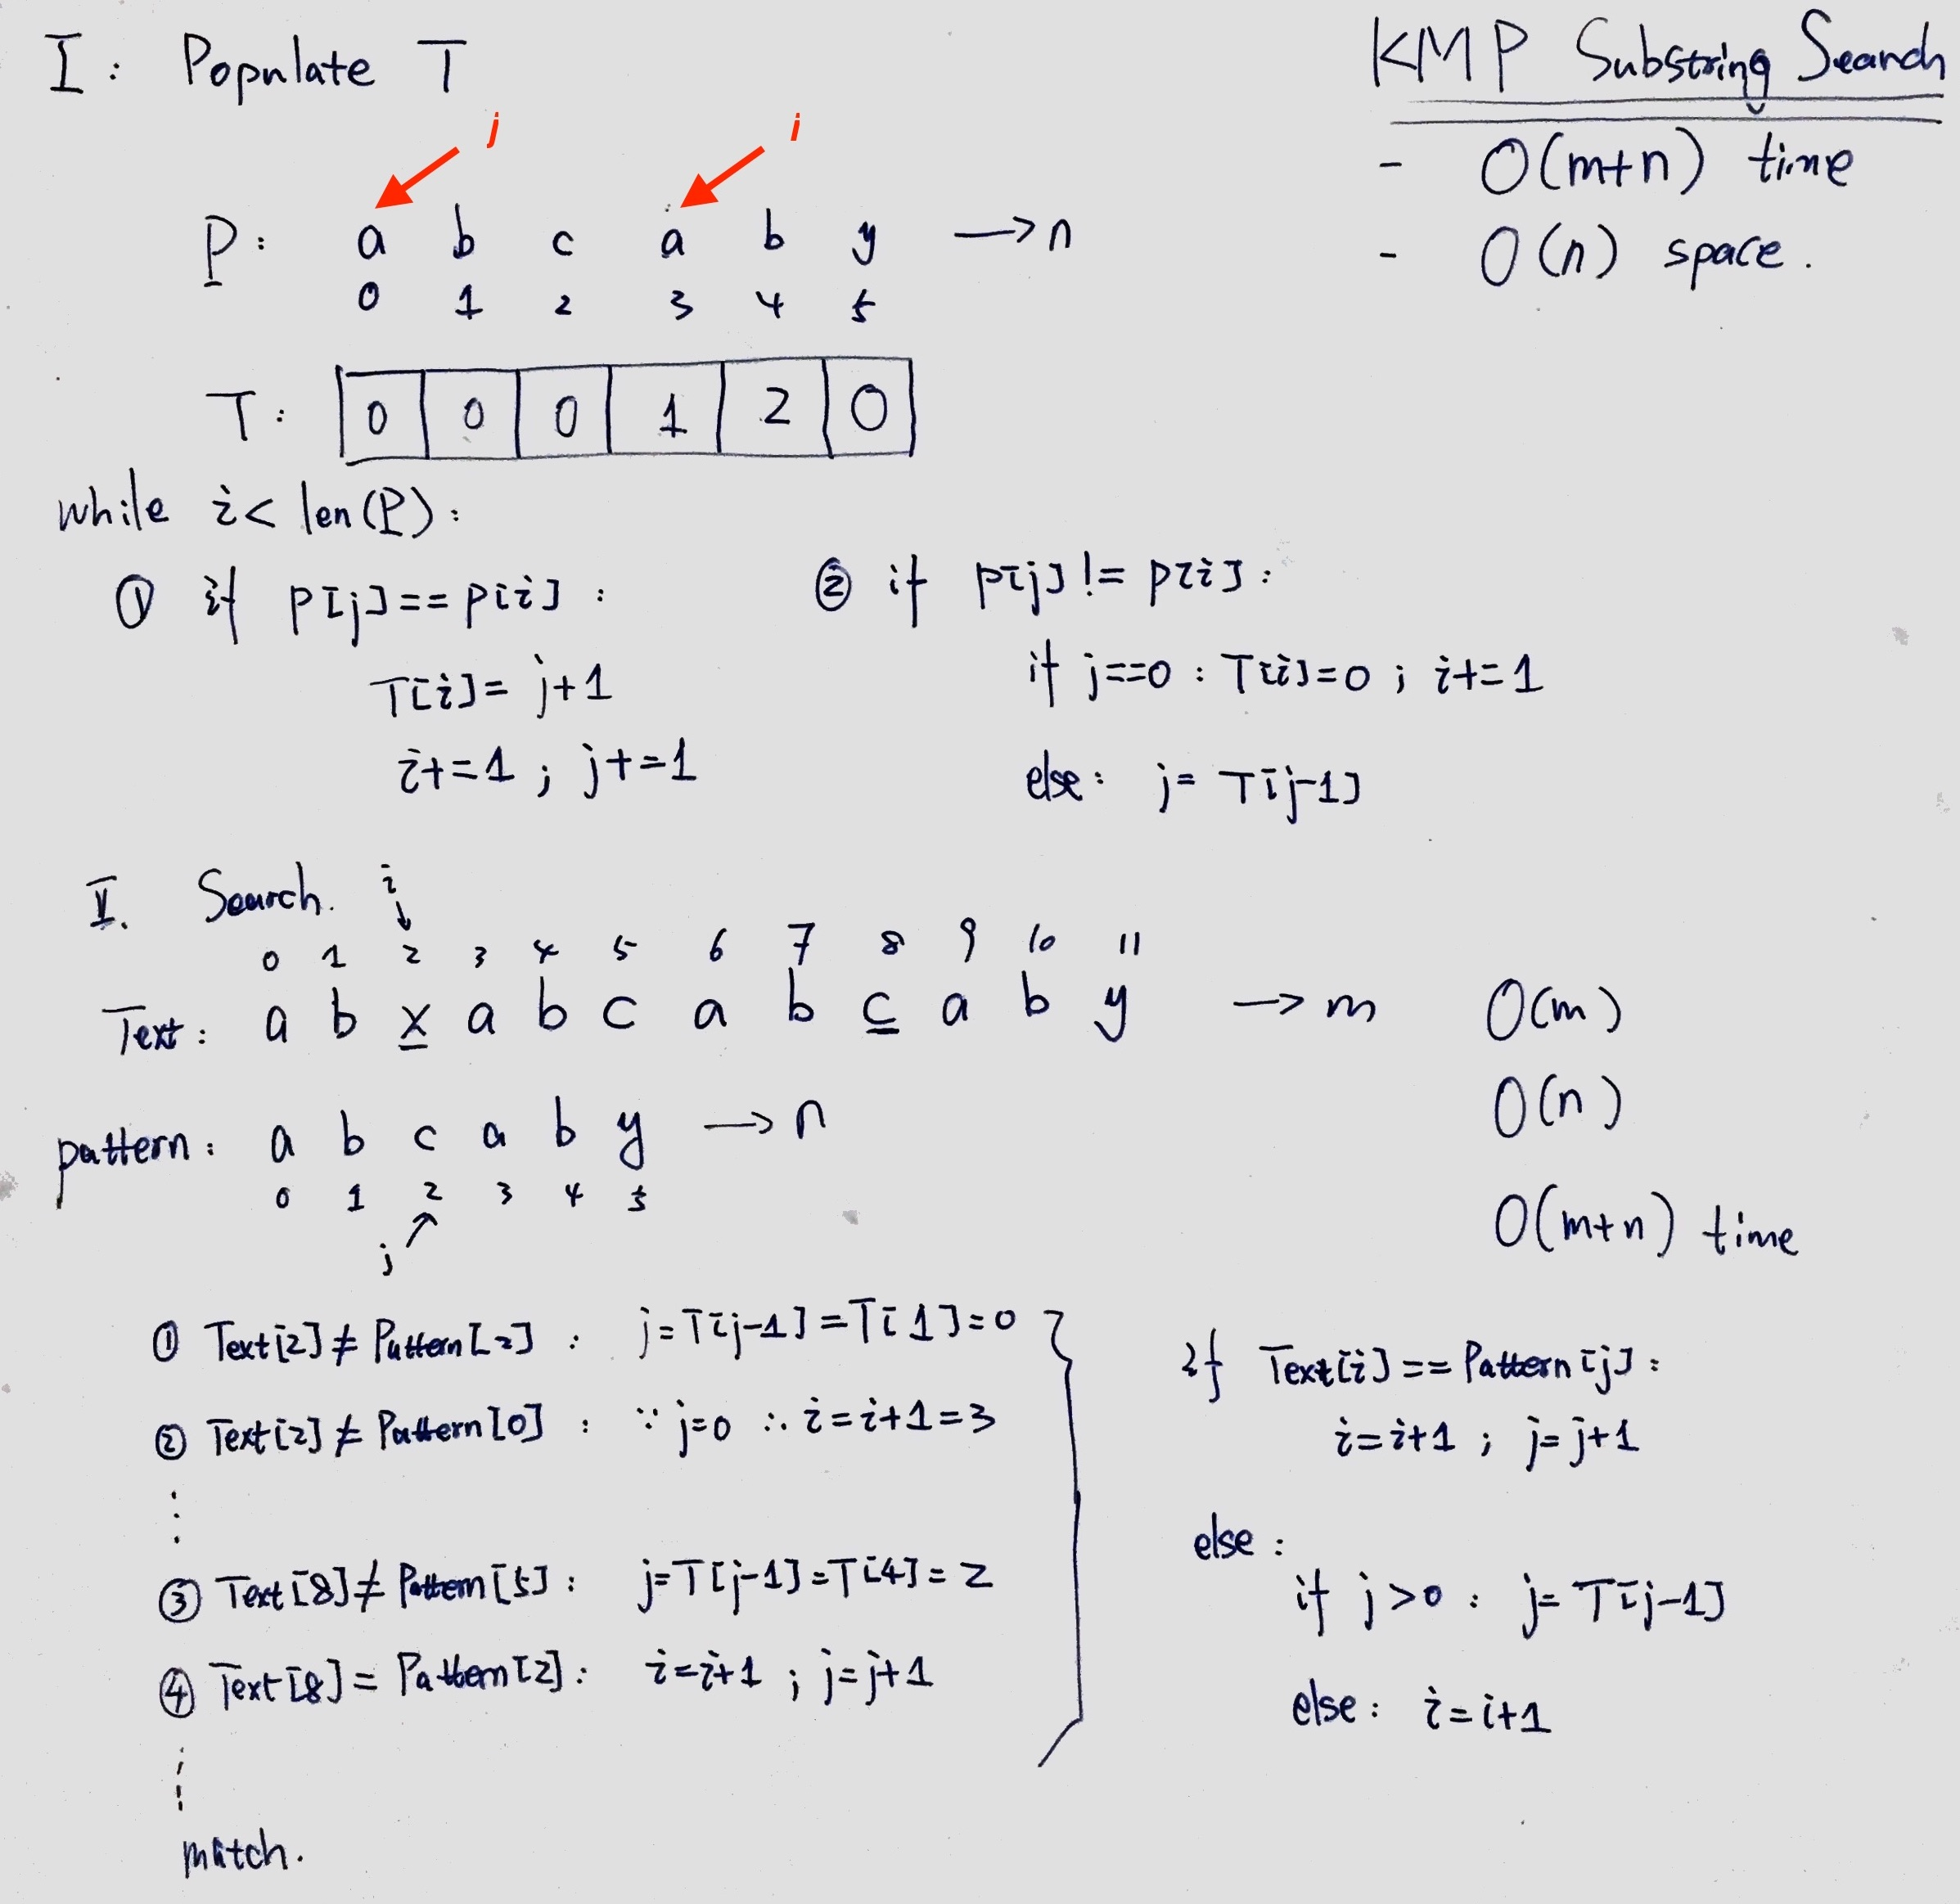
\includegraphics[width=\textwidth]{leetcode28-1.jpg}
    \centering \\
\end{figure}

\begin{figure}[h]
    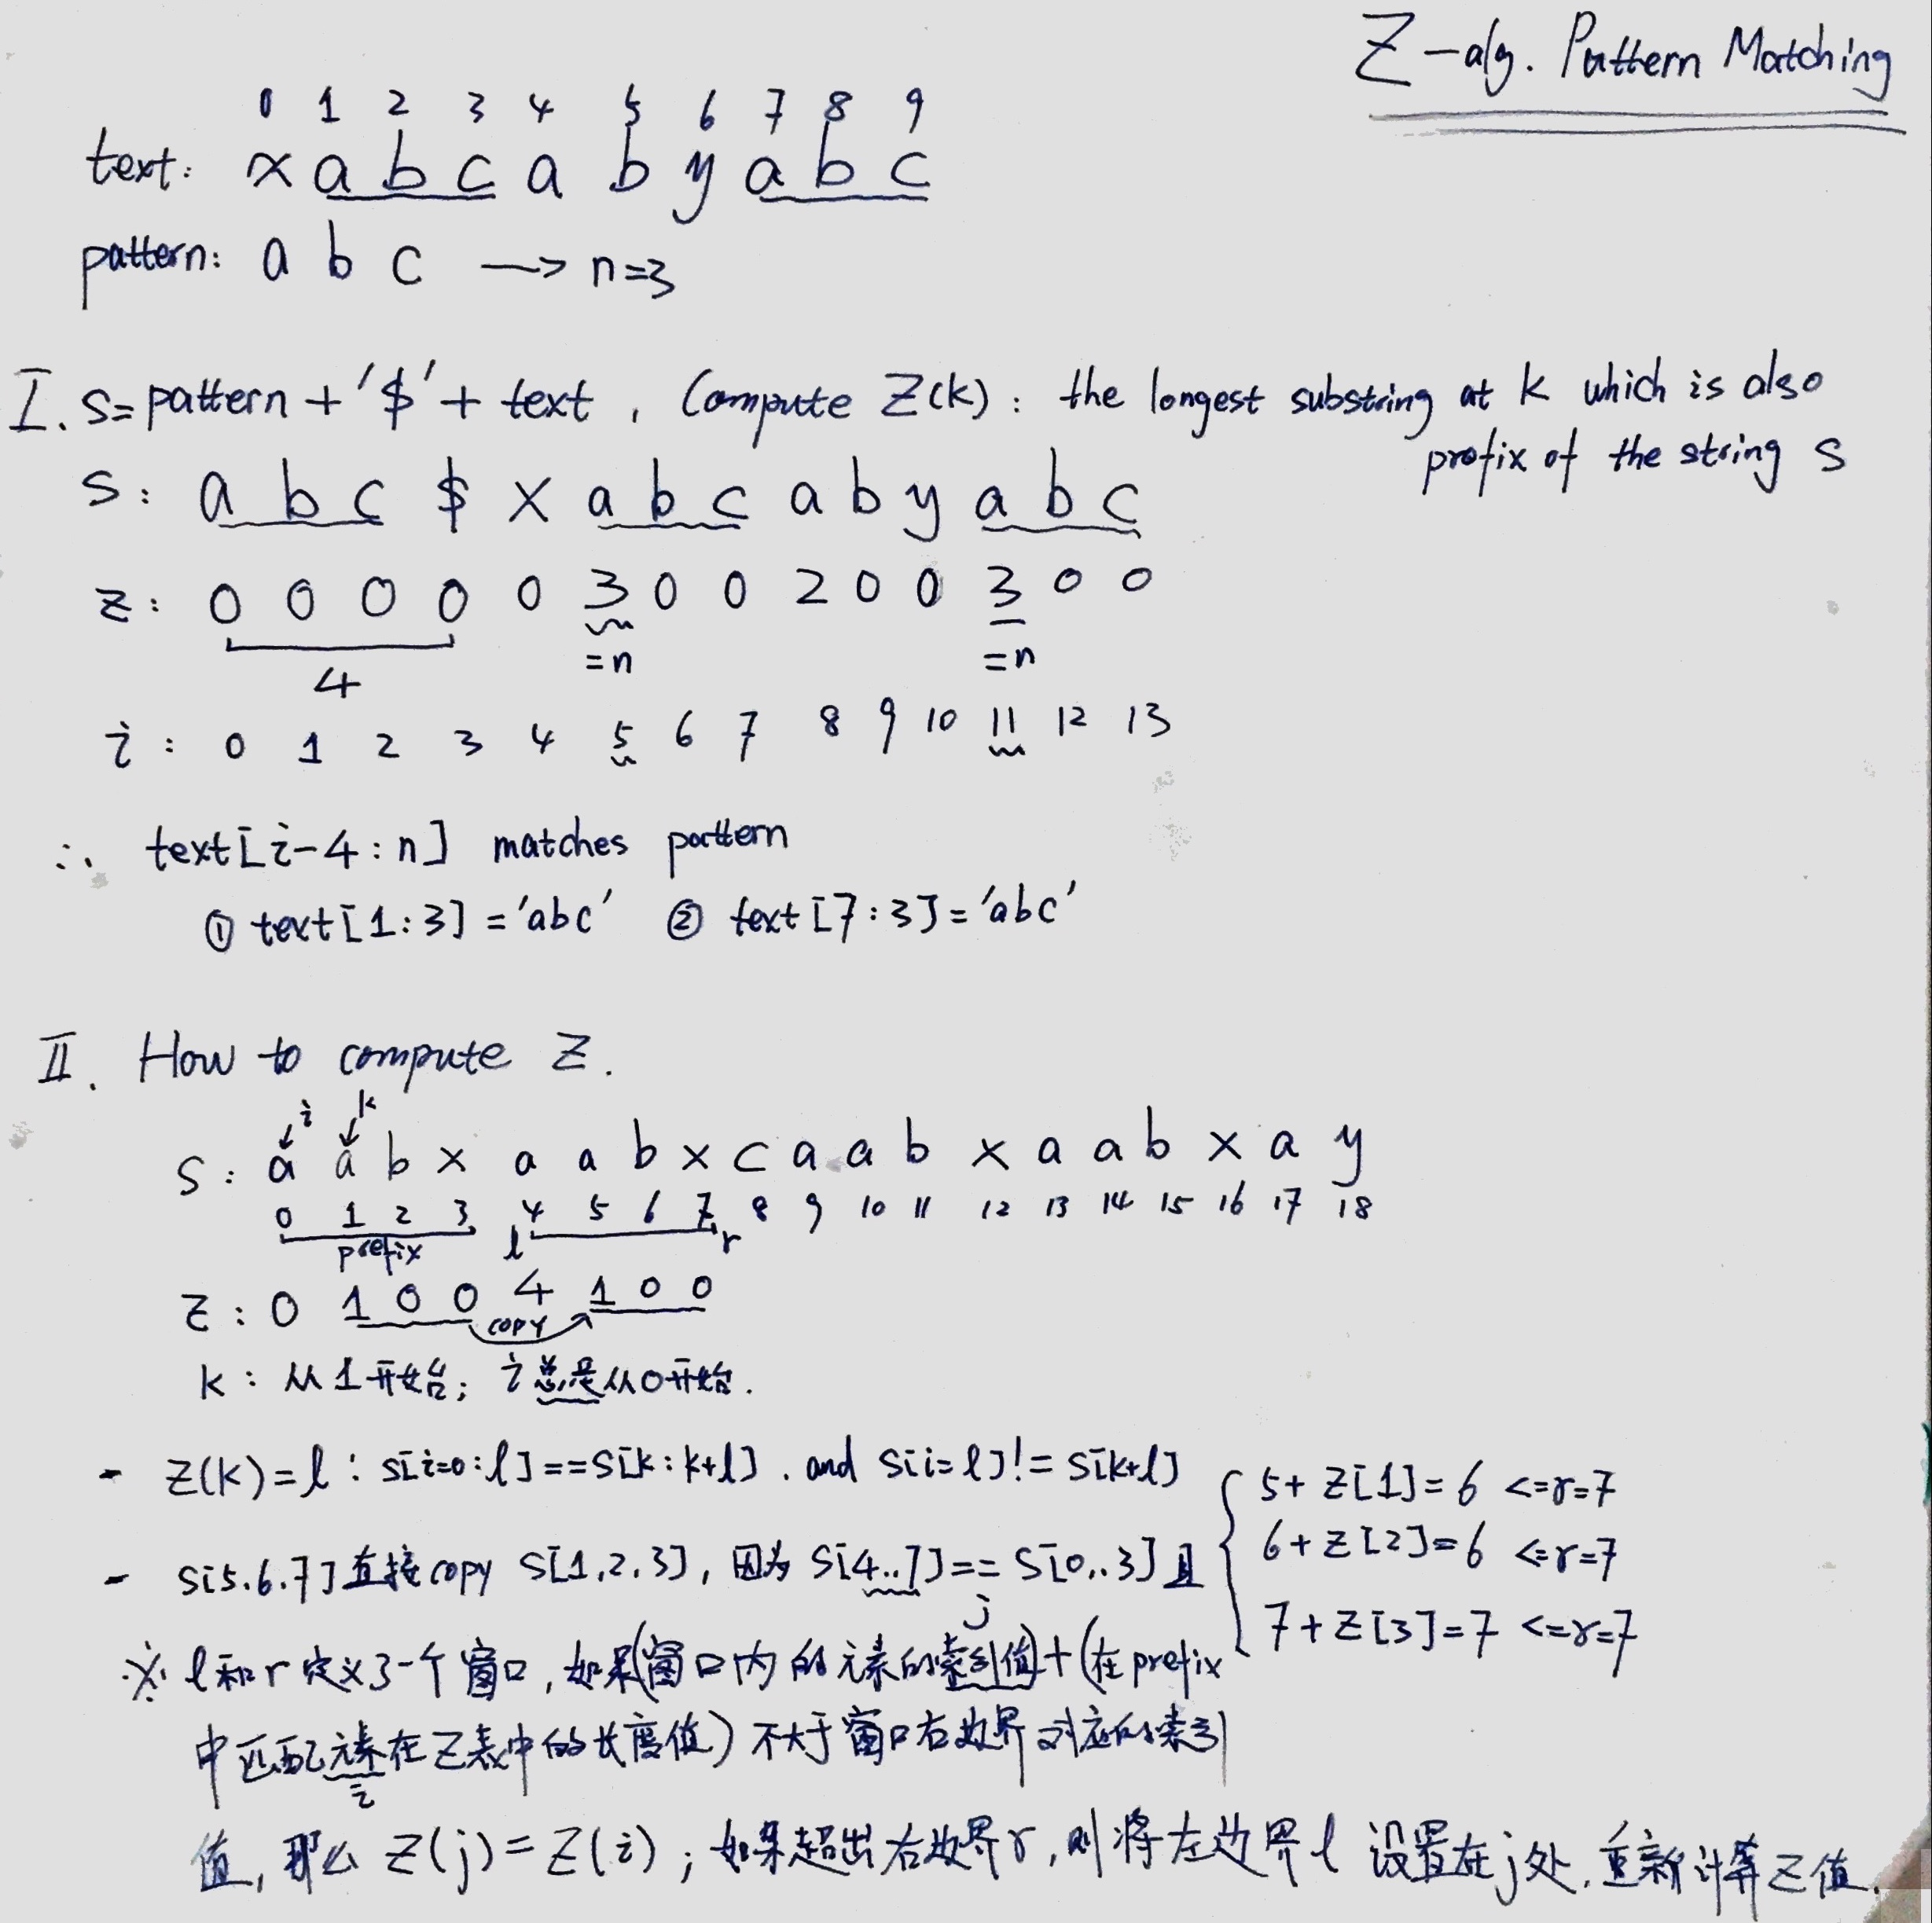
\includegraphics[width=\textwidth]{leetcode28-2.jpg}
    \centering \\
\end{figure}

\begin{figure}[h]
    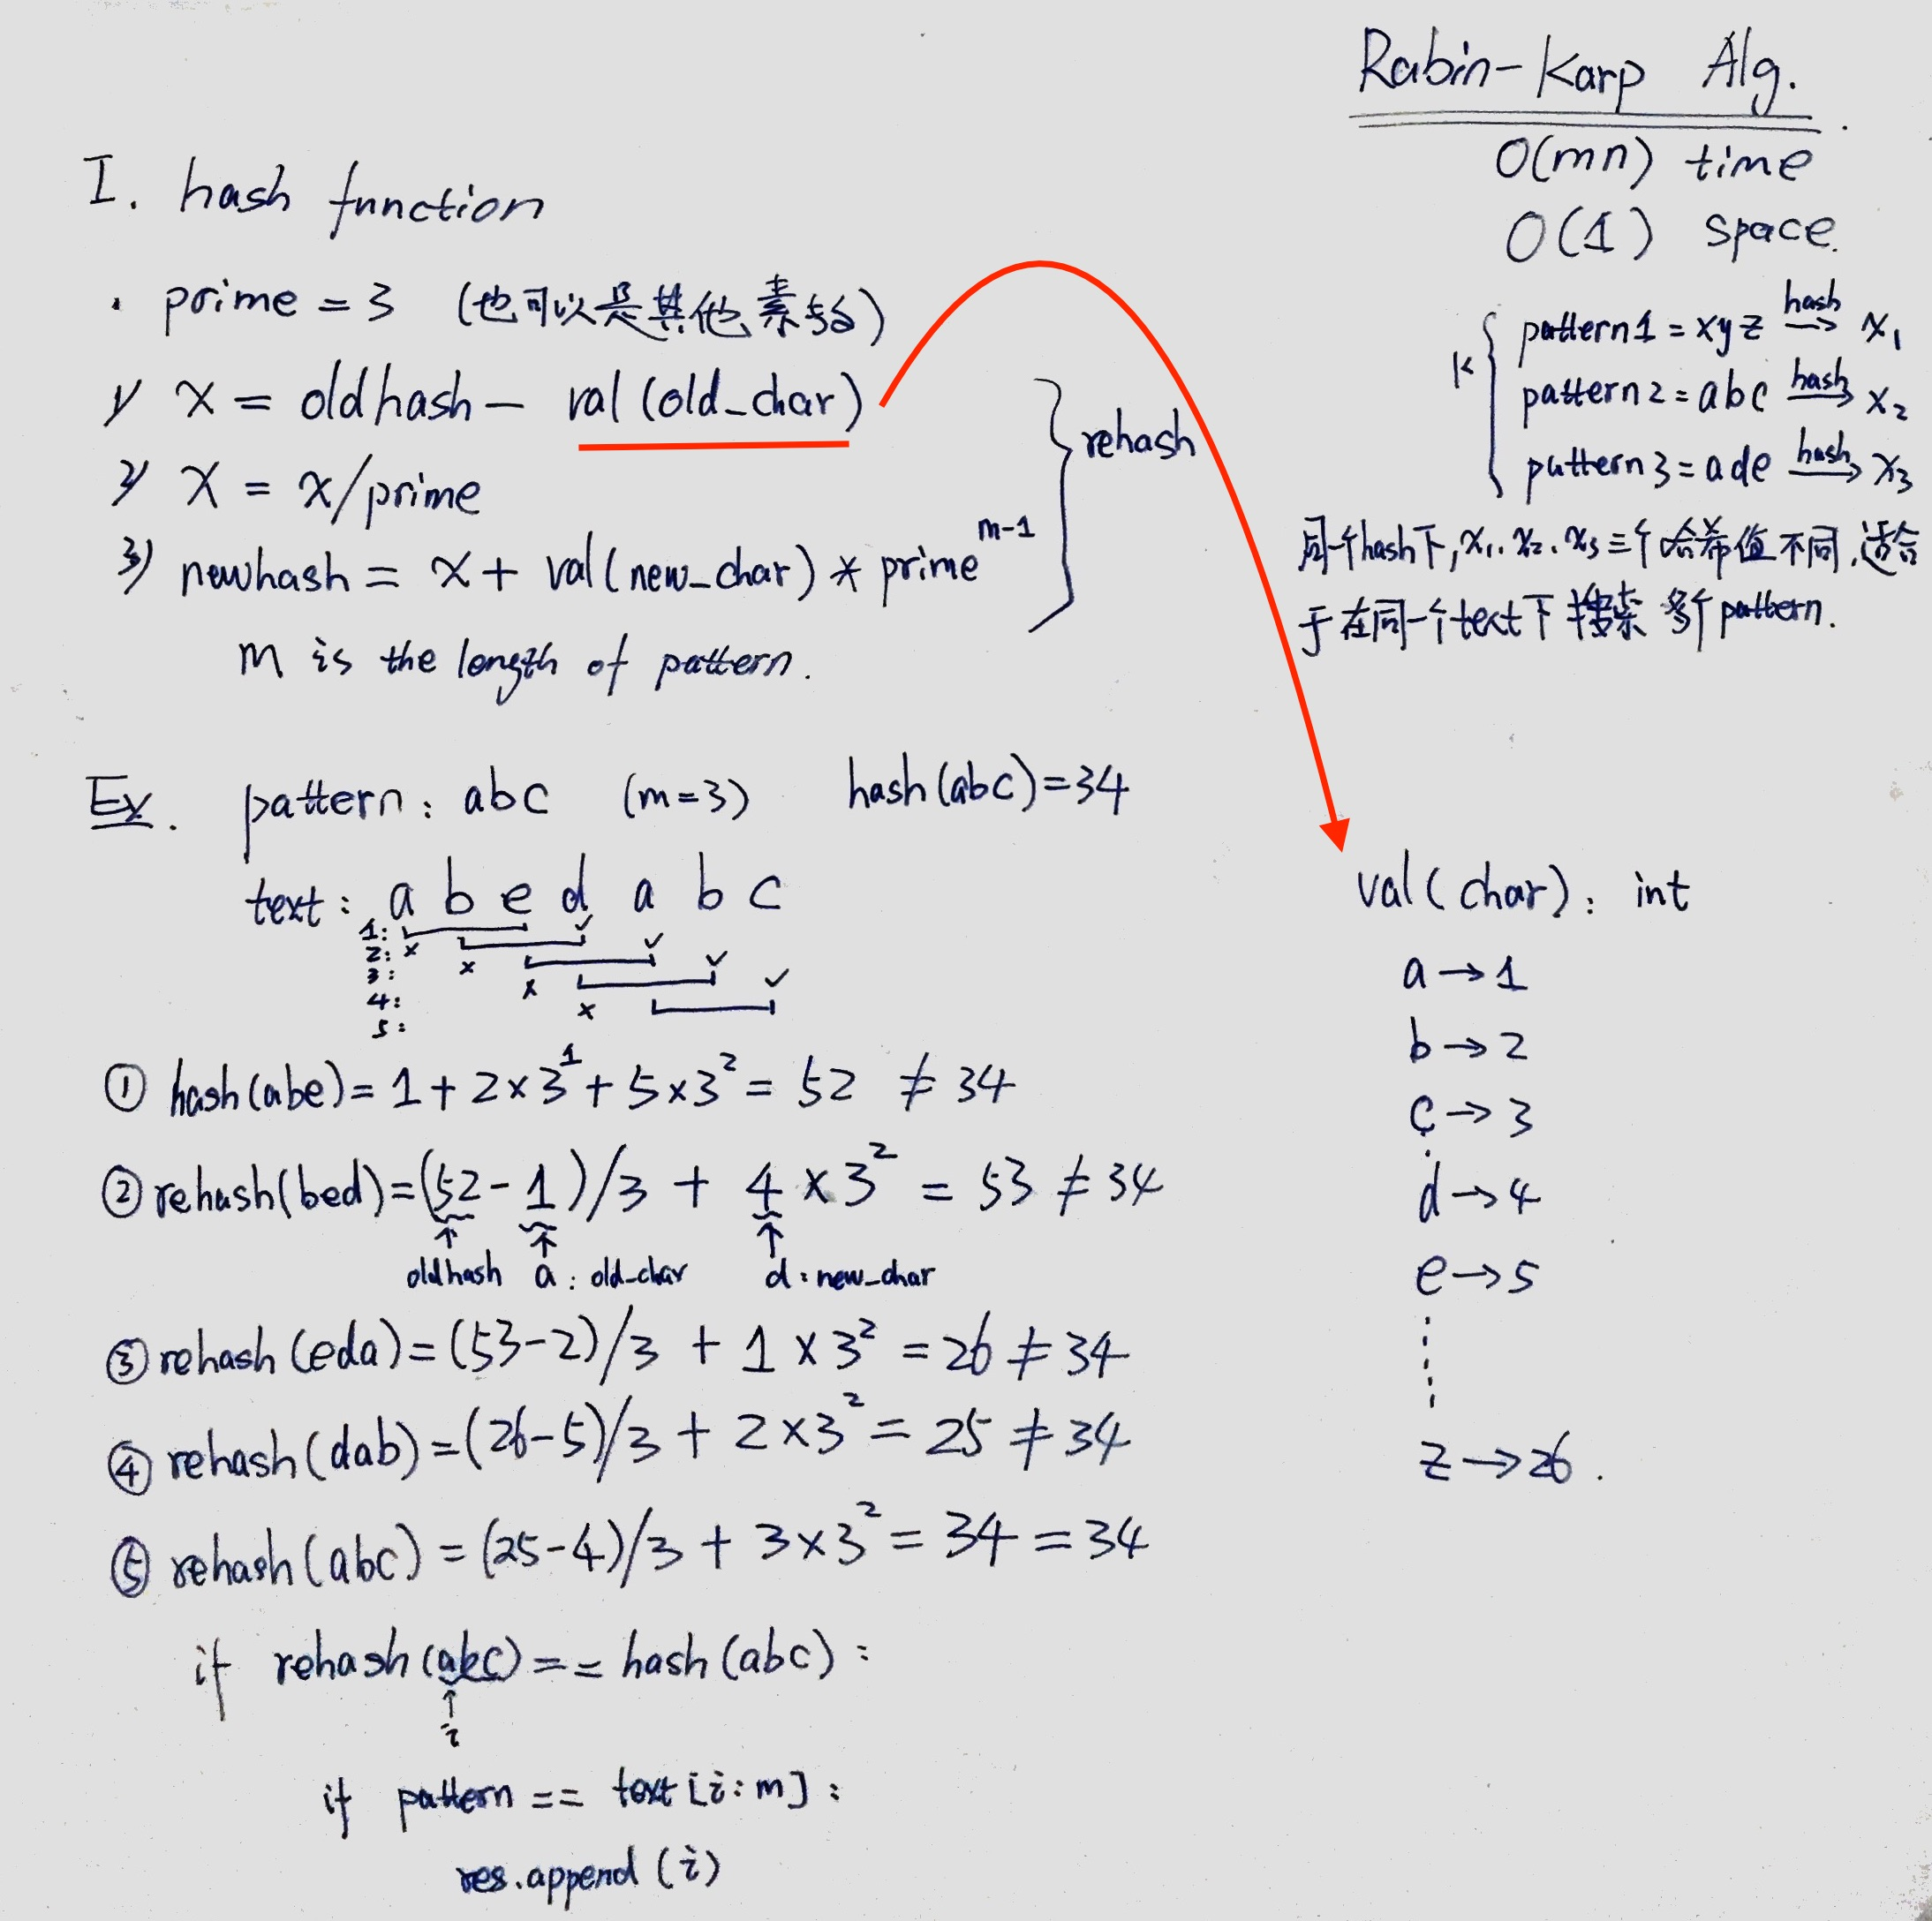
\includegraphics[width=\textwidth]{leetcode28-3.jpg}
    \centering \\
\end{figure}

\begin{lstlisting}[language=Python, caption=Problem28. Implement strStr()]

class Solution(object):
    def strStr_bruteforce(self, haystack, needle): # RT: O(mn)
        """
        :type haystack: str
        :type needle: str
        :rtype: int
        """
        m, n = len(haystack), len(needle)
        if n==0: return 0
        if m<n: return -1
        
        # the range is the most critical part for the performance
        for i in range(m-n+1): 
            if haystack[i:i+n]==needle:
                return i
        return -1
    
    def strStr_KMP(self, haystack, needle):  # O(m+n) time, O(n) space
        m, n = len(haystack), len(needle)
        if n == 0: return 0
        if m < n: return -1
        
        # traverse needle to fill out array T in O(n) time
        T = [0 for _ in xrange(n)]
        i, j = 1, 0
        while i < n:
            if needle[j] == needle[i]:
                T[i] = j + 1
                i += 1
                j += 1
            else:
                if j == 0:
                    T[i] = 0
                    i += 1
                else:
                    j = T[j-1]
        
        # traverse haystack in O(m) time
        i = j = 0
        while i < m and j < n:
            if haystack[i] == needle[j]:
                i += 1
                j += 1
            else:
                if j > 0:
                    j = T[j-1]
                else:
                    i += 1
        if j == n:
            return i - n
        else:
            return -1
    
    def strStr_Z(self, haystack, needle):  # O(m+n) time, O(m+n) space

        m, n = len(haystack), len(needle)
        if n == 0: return 0
        if m < n: return -1

        text = needle + '$' + haystack
        size = m + n + 1

        Z = self.calculate_Z(text)

        res = [i-n-1 for i in xrange(size) if Z[i] == n]

        if res == []:
            return -1
        else:
            return res[0]

    def calculate_Z(self, text):
        size = len(text)
        Z = [0 for _ in xrange(size)]
        # left bound and right bound
        left, right = 0, 0

        for k in xrange(1, size):
            if k == 13:
                pass
            if k > right:
                left = right = k
                while right < len(text) and text[right] == text[right-left]:
                    right += 1
                Z[k] = right-left
                right -= 1
            else:
                # operate inside box
                k1 = k - left
                # if value does not stretches till right bound, then just copy it
                if k+Z[k1] <= right:
                    Z[k] = Z[k1]
                else:
                    # try to see if there are more matches
                    left = k
                    while right < size and text[right] == text[right-left]:
                        right += 1
                    Z[k] = right-left
                    right -= 1
        return Z
    
    def strStr_RabinKarp(self, haystack, needle):  # O(m*n) time, O(1) space
        """
        :type haystack: str
        :type needle: str
        :rtype: int
        """
        m, n = len(haystack), len(needle)
        if n == 0: return 0
        if m < n: return -1

        keys = list('abcdefghijklmnopqrstuvwxyz')
        values = [i+1 for i in xrange(26)]
        self.value_dict = dict(zip(keys, values))

        # set up a prim number, which can be any prime number
        prime = 3
        # compute the hash number of the pattern, needle
        hash_needle = self.get_hash(needle, prime)

        res = []
        hash_value = self.get_hash(haystack[0:n], prime)
        if hash_needle == hash_value:
            res.append(0)
        for i in xrange(1, m-n+1):
            hash_value = (hash_value - self.value_dict[haystack[i-1]]) / prime
            hash_value += self.value_dict[haystack[i+n-1]] * pow(prime, (n-1))
            if hash_needle == hash_value:
                res.append(i)

        if res == []:
            return -1
        else:
            return res[0]

    def get_hash(self, text, prime):
        hashcode = 0
        for i in xrange(len(text)):
            hashcode += self.value_dict[text[i]] * pow(prime, i)
        return hashcode
\end{lstlisting}



\subsection{leetcode 8. String to Integer (atoi)}
Implement atoi to convert a string to an integer.\\

\noindent Notes: It is intended for this problem to be specified vaguely (ie, no given input specs). You are responsible to gather all the input requirements up front. \\

\noindent Requirements for atoi:
\begin{itemize}
    \item The function first discards as many whitespace characters as necessary until the first non-whitespace character is found. Then, starting from this character, takes an optional initial plus or minus sign followed by as many numerical digits as possible, and interprets them as a numerical value.
    \item The string can contain additional characters after those that form the integral number, which are ignored and have no effect on the behavior of this function.
    \item If the first sequence of non-whitespace characters in str is not a valid integral number, or if no such sequence exists because either str is empty or it contains only whitespace characters, no conversion is performed.
    \item If no valid conversion could be performed, a zero value is returned. If the correct value is out of the range of representable values, 2147483647 or -2147483648 is returned.
\end{itemize}

\begin{CJK*}{UTF8}{gbsn}
\noindent 解题思路:需要特别注意这道题!!!题目的难度不大,但是需要考虑很多边界情况和特殊情况。需要注意以下几点:
\begin{enumerate}
    \item 32位整数的上下界:-2147483648 ~ 2147483647;
    \item 字符串长度为0时应该返回什么值。
    \item 正负号的处理;
    \item 字符串前面(leading)和后面(trailing)的空白字符;
    \item 除了字符串开头的正负号以外,其他的字符对应的ascii应该在48~57范围以内。
\end{enumerate}
\end{CJK*}

\begin{lstlisting}[language=Python, caption=Problem8. String to Integer (atoi)]

class Solution(object):
    def myAtoi(self, str):
        """
        :type str: str
        :rtype: int
        """
        if len(str)==0: return 0
        
        # remove the leading and tailing whitespace
        s = str.strip()
        
        # 0: positive, 1: negative
        neg = 0 
        if s[0]=="+" or s[0]=="-": 
            if s[0]=="-": neg=1
            s=s[1:]
        lowerbound, upperbound = -2147483648, 2147483647
        res = 0
        for i in xrange(len(s)):
            if ord(s[i])<48 or ord(s[i])>57: 
                return res
            res = res*10 + pow(-1,neg)*(ord(s[i])-48)
            if res<0 and res<=lowerbound: 
                return lowerbound
            elif res>0 and res>=upperbound: 
                return upperbound
        return res
\end{lstlisting}

\begin{figure}[h]
    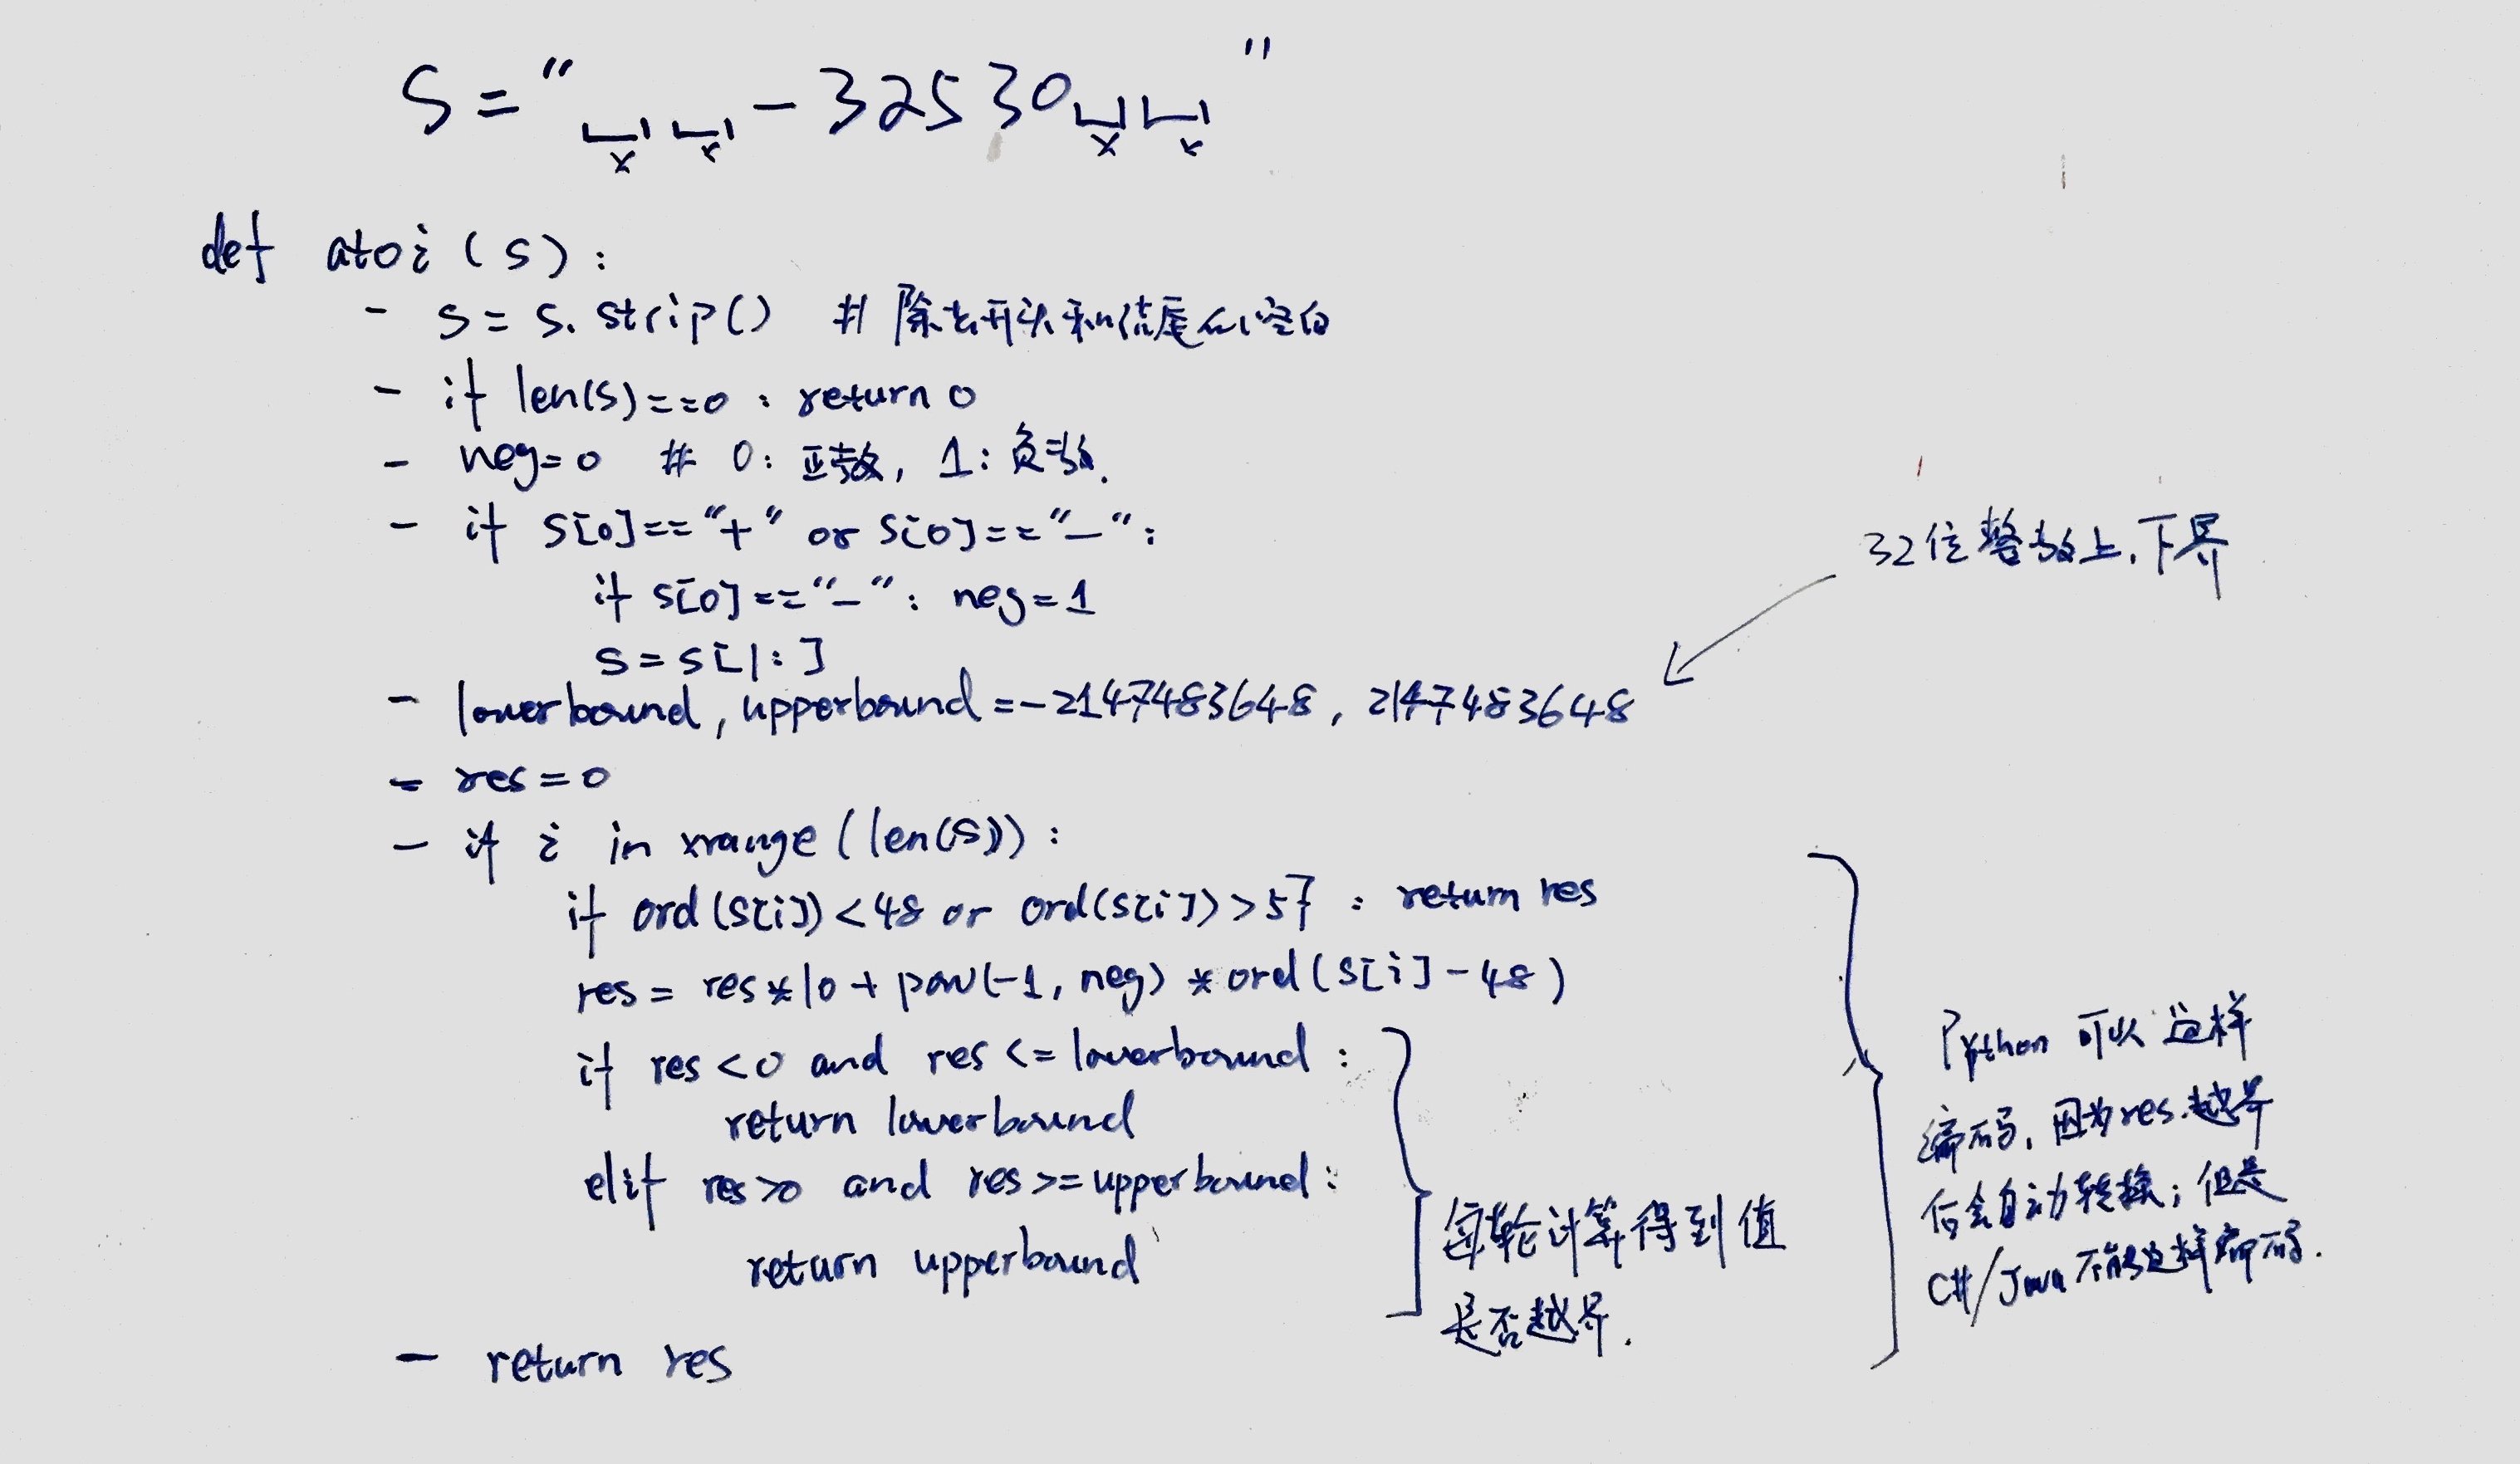
\includegraphics[width=\textwidth]{leetcode8.jpg}
    \centering \\
\end{figure}





\subsection{leetcode 67. Add Binary}
Given two binary strings, return their sum (also a binary string). For example, a = "11", b = "1", return "100". \\

\begin{CJK*}{UTF8}{gbsn}
\noindent 解题思路:这道题不难,但是用python实现的时候需要注意\textbf{string类型的数据是没法通过索引进行更新的},即无法完成a[i]="x"这样的赋值语句。如果想操作数据,就需要先转换成list类型。注意,为了方便,示例图中的代码,$a$和$b$是list类型,并且list中的是数值而不是字符。\\
\end{CJK*}

\begin{lstlisting}[language=Python, caption=Problem67. Add Binary]

class Solution(object):
    def addBinary(self, a, b):
        """
        :type a: str
        :type b: str
        :rtype: str
        """
        if a=="": return b
        elif b=="": return a
        
        if len(a)<len(b): a,b=b,a
        
        alist=list(a)
        blist=list(b)
        carry=0
        for i in range(-1, -len(blist)-1, -1):
            if alist[i]=='1' and blist[i]=='1':
                alist[i]=str(carry)
                carry=1
            elif alist[i]=='0' and blist[i]=='0':
                alist[i]=str(carry)
                carry=0
            else: # (a[i]=='1' and b[i]=='0') or (a[i]=='0' and b[i]=='1')
                alist[i]= str((1+carry)%2)
                carry=(1+carry)/2  # Bug: carry=0
        
        j=-len(blist)-1
        while carry==1 and j>=-len(alist):
            if alist[j]=='1':
                alist[j]=str(0)
                carry=1
                j-=1
            else:
                alist[j]=str(1)
                carry=0
                break

        if carry==1 and j<-len(alist):
            return "".join(["1"] + alist)
        else:
            return "".join(alist)
\end{lstlisting}

\begin{figure}[h]
    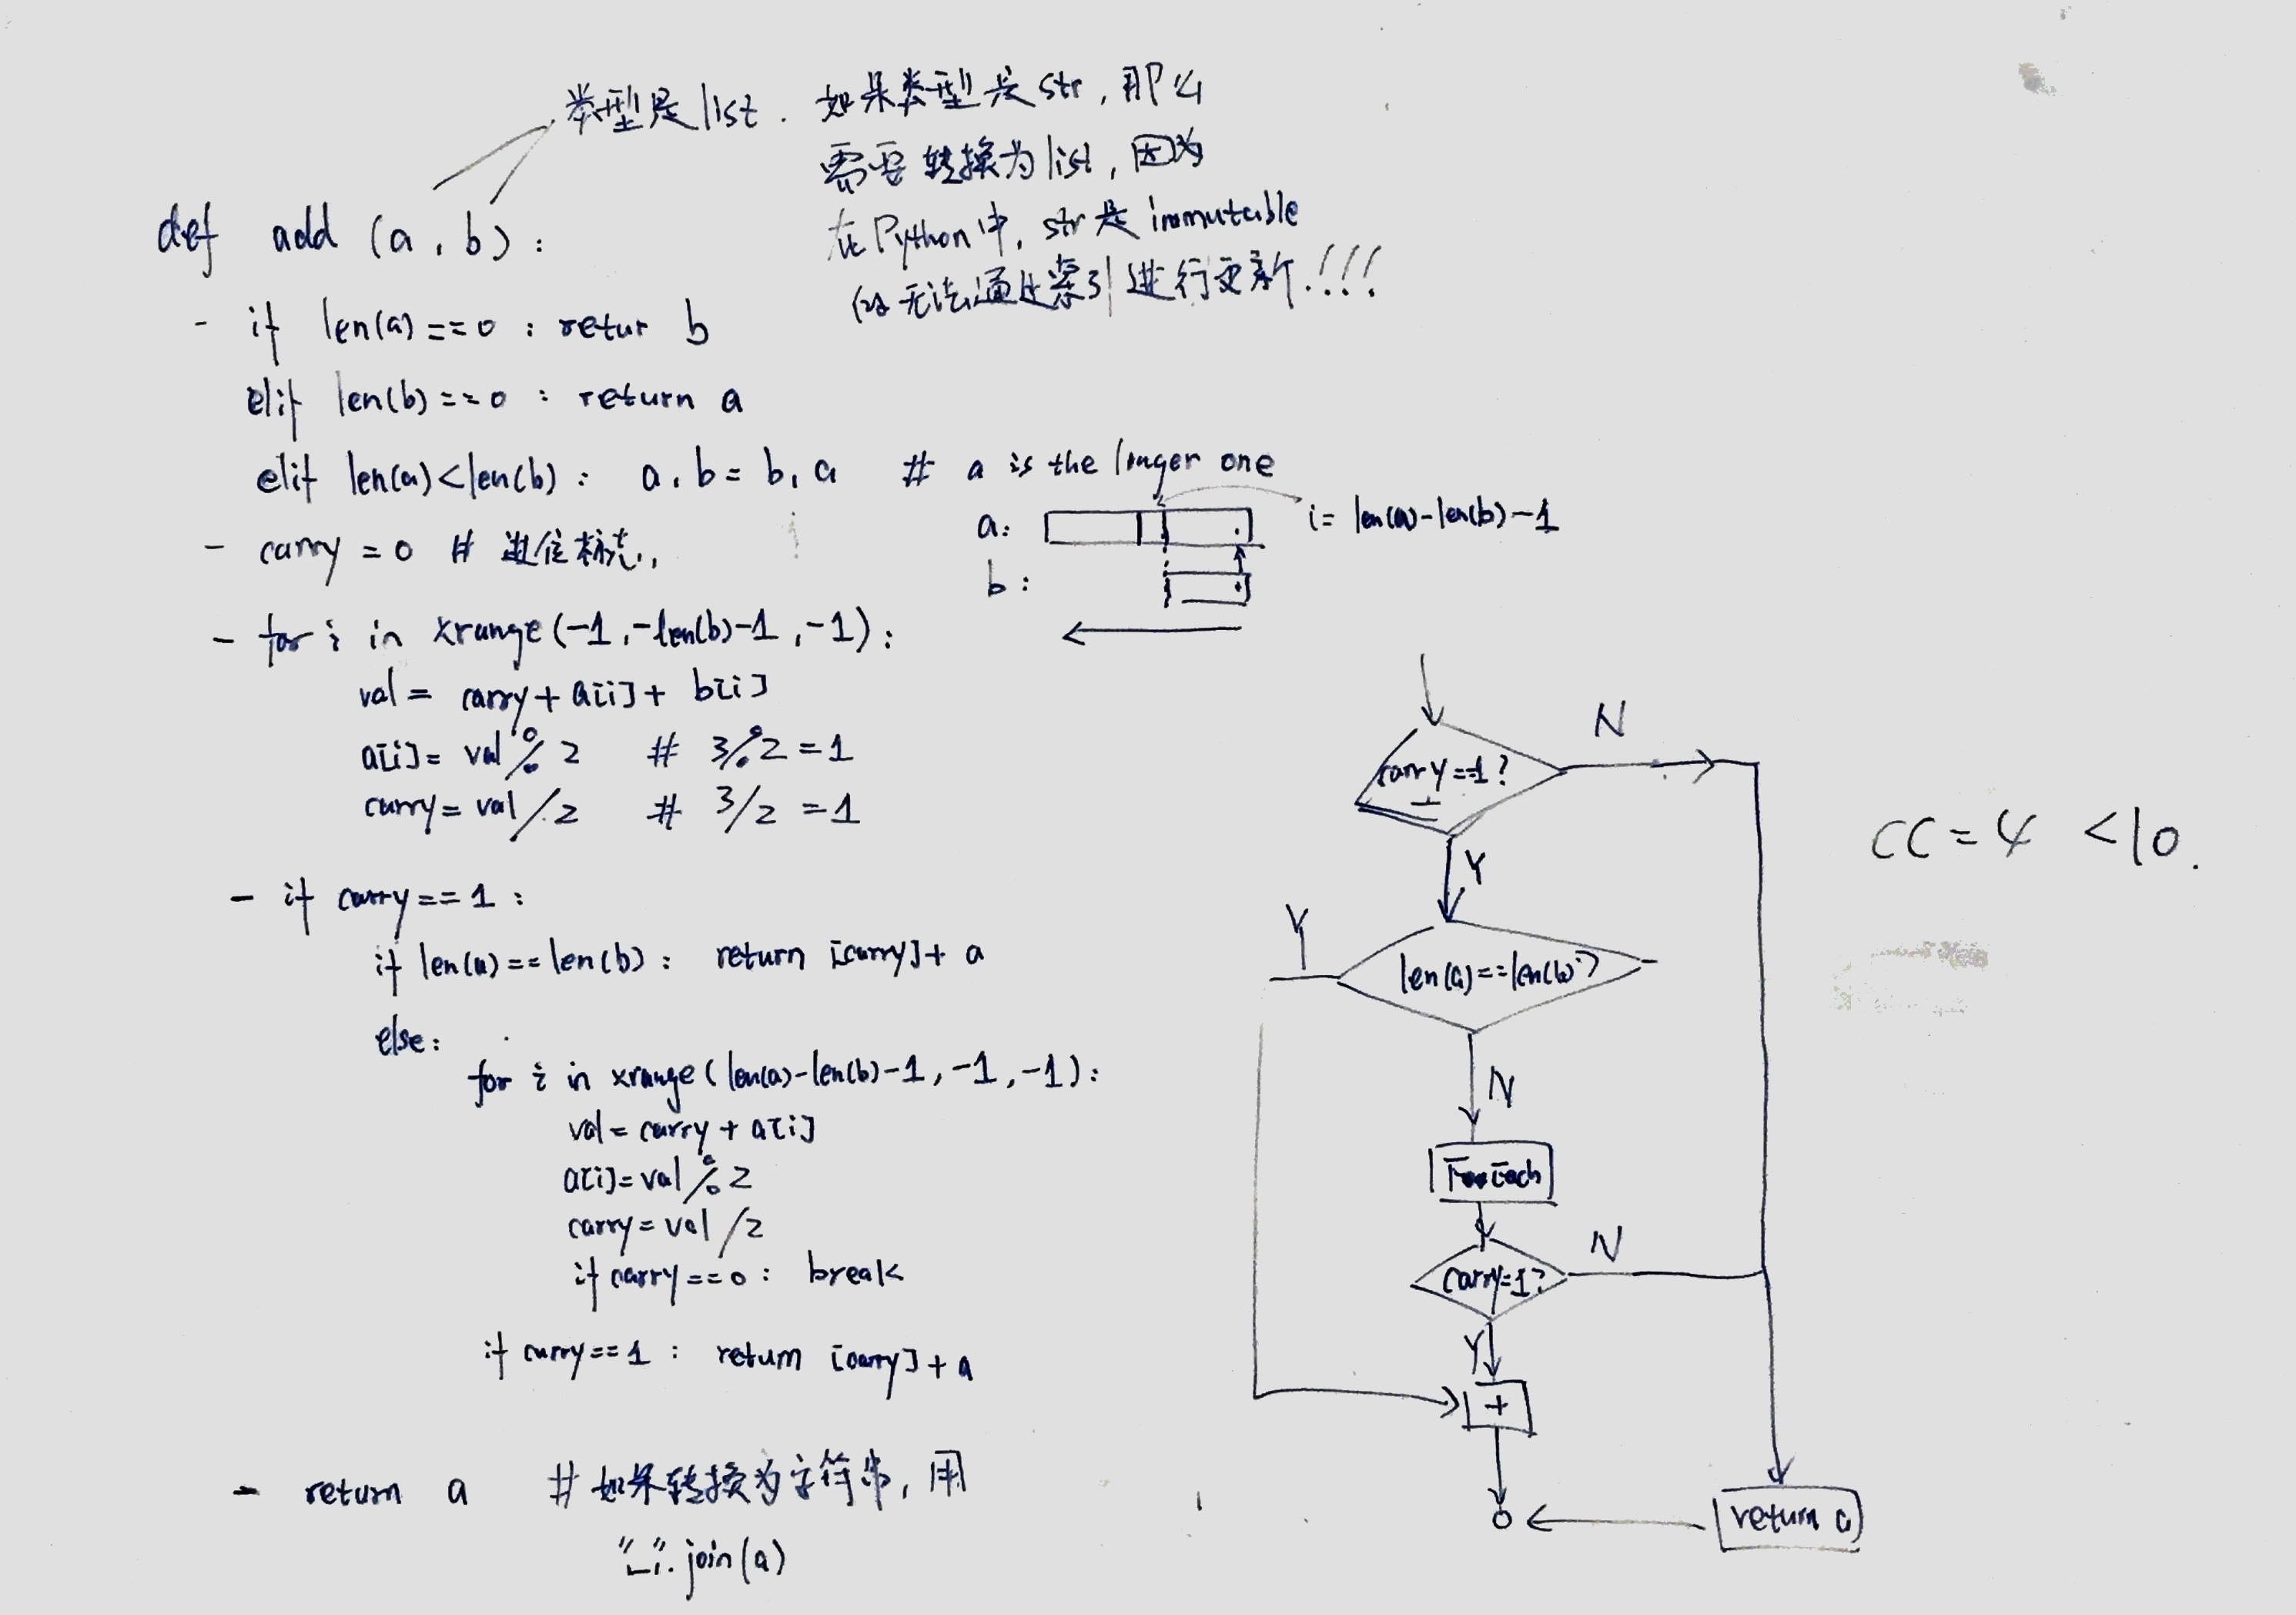
\includegraphics[width=\textwidth]{leetcode67.jpg}
    \centering \\
\end{figure}




\subsection{leetcode 5. Longest Palindromic Substring}
Given a string S, find the longest palindromic substring in S. You may assume that the maximum length of S is 1000, and there exists one unique longest palindromic substring. \\

\begin{CJK*}{UTF8}{gbsn}
\noindent 有两个帖子对这个问题的解法有很好的讨论:http://articles.leetcode.com/longest-palindromic-substring-part-i 和 http://articles.leetcode.com/longest-palindromic-substring-part-ii。\\

\noindent 这个题共计有四种解法:
\begin{itemize}
    \item 第一种解法:brute-force暴力算法,时间复杂度为$O(n^3)$。每次在$n$长的字符串中选择两个字符作为子串的起点和终点,共有$\frac{n(n-1)}{2}$种选择,而检查每种选择的子串是否为palindrome需要$O(n)$的时间复杂度,所以整个算法的时间复杂度为$O(n^3)$。
    
    \item 第二种解法:dynamic programming,时间复杂度为$O(n^2)$用于填充矩阵,空间复杂度为$O(n^2)$用于存储中间结果的矩阵。dp[i][j]表示索引$i$和$j$之间的子串是否为回文。状态转换方程的定义及示例见第一个示例图。
    
    \item 第三种解法:在第二种算法的基础上,减少空间复杂度至$O(1)$,时间复杂度不变。算法的思路是每个回文都是从中间元素为中心两侧对称的字符串,而中心点可能是某个字符也可能是两个字符中间的位置。对于一个长度为$n$的字符串,这样的中心点有$2n-1$个:有$n$个字符,每个字符为一个;另外,$n$个字符中,每两个字符中间的位置为一个中心点,这样的位置有$n-1$个。依次以这$2n-1$个位置为中心点对字符串进行扩展和判定,获得最大回文子串。每次扩展最多为$O(n)$,所以总的时间复杂度为$O(n^2)$
    
    \item 第四种解法:Manacher's algorithm. 该算法的核心是利用回文字符串的对称性减少计算量。算法需要预处理字符串:在字符串的首尾和两两字符间插入一个特殊字符“#”。该算法的详解见http://articles.leetcode.com/longest-palindromic-substring-part-i/。示例和演算参考第二个示例图。
\end{itemize}
\end{CJK*}\\


\begin{lstlisting}[language=Python, caption=Problem5. Longest Palindromic Substring]

class Solution(object):

    def longestPalindrome_DP1(self, s): # RT: O(n^2) TLE error, Space: O(n^2)
        n = len(s)
        dp = [[False]*n for _ in xrange(n)]
        for x in xrange(n):
            dp[x][x] = True
        for x in xrange(n-1):
            if s[x]==s[x+1]:
                dp[x][x+1] = True
        maxlength = 0
        idx = 0
        for length in xrange(3,n+1):
            for x in xrange(n-length+1):
                y = x+length-1
                if s[x]==s[y] and dp[x+1][y-1]:
                    dp[x][y] = True
                    if maxlength < length:
                        maxlength = length
                        idx = x
        return s[idx:idx+maxlength]

    def longestPalindrome_DP2(self, s): # RT: O(n^2), Space: O(1)
        def expandAroundCenter(s, c1, c2):
            l, r = c1, c2
            n = len(s)
            while l>=0 and r<=n-1 and s[l]==s[r]:
                l-=1; r+=1
            return s[l+1:r]
            
        n = len(s)
        if n==0: return ""
        maxstring = s[0]
        for x in xrange(1, n):
            substring = expandAroundCenter(s, x-1, x)
            if len(maxstring)<len(substring):
                maxstring = substring
            
            substring = expandAroundCenter(s, x, x)
            if len(maxstring)<len(substring):
                maxstring = substring
        return maxstring
    
    def longestPalindrome_manacher(self, s):  # RT: O(n), Space: O(n)

        def preprocess(s):  # O(n) time
            """
            Insert '#' into the original string between every two characters:
                '^' denotes the starting position of the new string,
                '$' denotes the ending position of the new string.
            """
            n = len(s)
            if n == 0: return "^$"
            res = "^"
            for x in xrange(n):
                res += "#" + s[x]
            res += "#$"
            return res

        T = preprocess(s)
        n = len(T)

        # dp[x] denotes the length of the longest palindrome centered at T[x]
        dp = [0 for _ in xrange(n)]

        center, rightEdge = 0, 0
        for x in xrange(1, n-1):
            # x'=center-(x-center)
            x_mirror = 2*center-x

            dp[x] = min(rightEdge-x, dp[x_mirror]) if rightEdge > x else 0

            # attempt to expand palindrome centers at x
            while T[x+dp[x]+1] == T[x-dp[x]-1]:
                dp[x] += 1

            # If palindrome centered at x expand past rightEdge,
            # update center and rightEdge based on expanded palindrome
            if x+dp[x] > rightEdge:
                center = x
                rightEdge = x+dp[x]

        # find the maximum element in dp
        maxlen = 0
        centeridx = 0
        for x in xrange(1, n-1):
            if maxlen < dp[x]:
                maxlen = dp[x]
                centeridx = x
        
        # being divided by 2 means removing '#' characters
        start = (centeridx-maxlen-1)/2
        return s[start:start+maxlen]
\end{lstlisting}

\begin{figure}[h]
    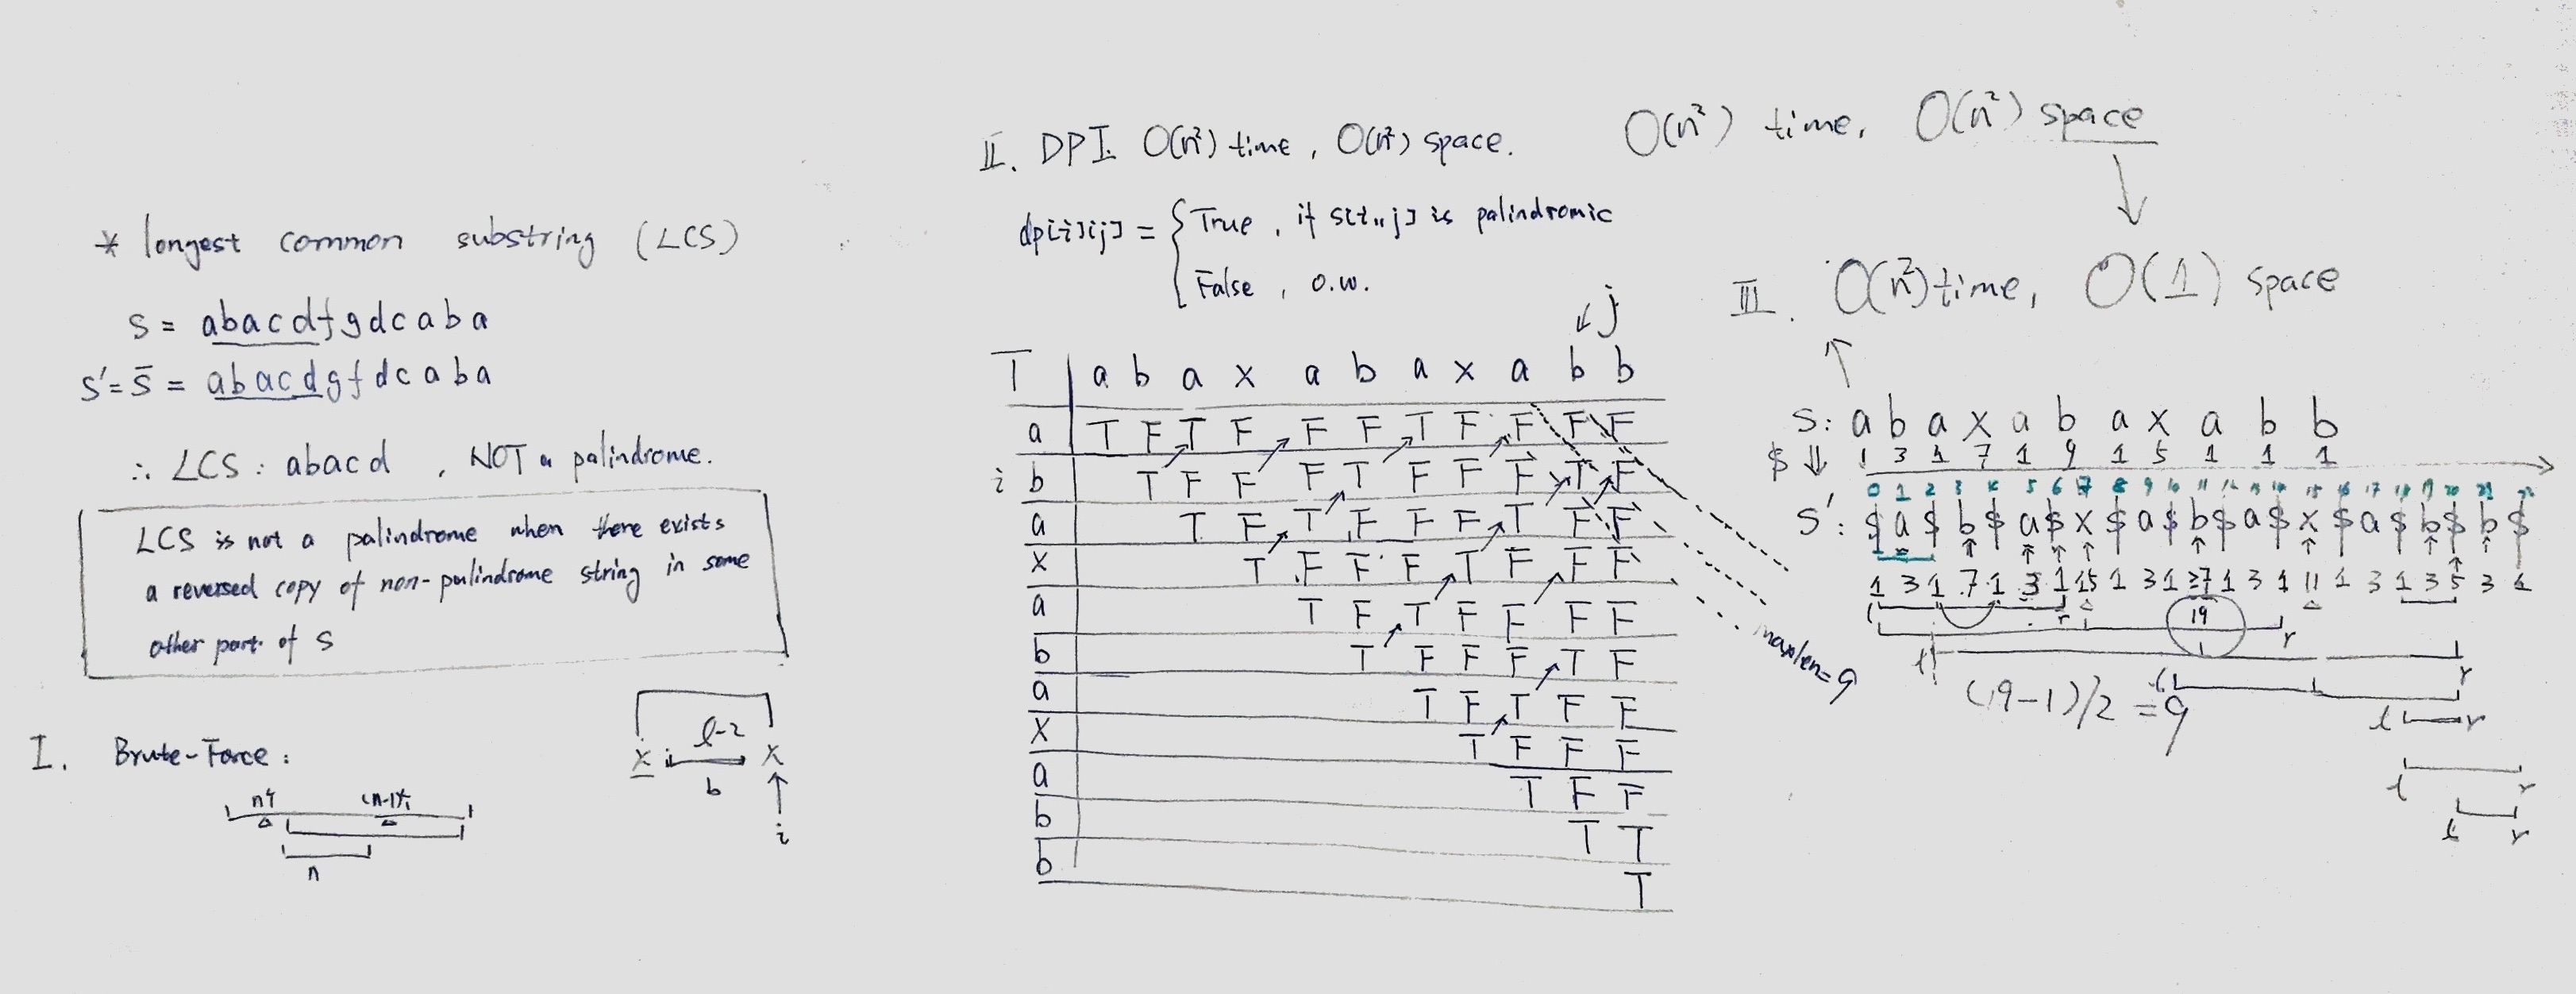
\includegraphics[width=\textwidth]{leetcode5-1.jpg}
    \centering
\end{figure}

\begin{figure}[h]
    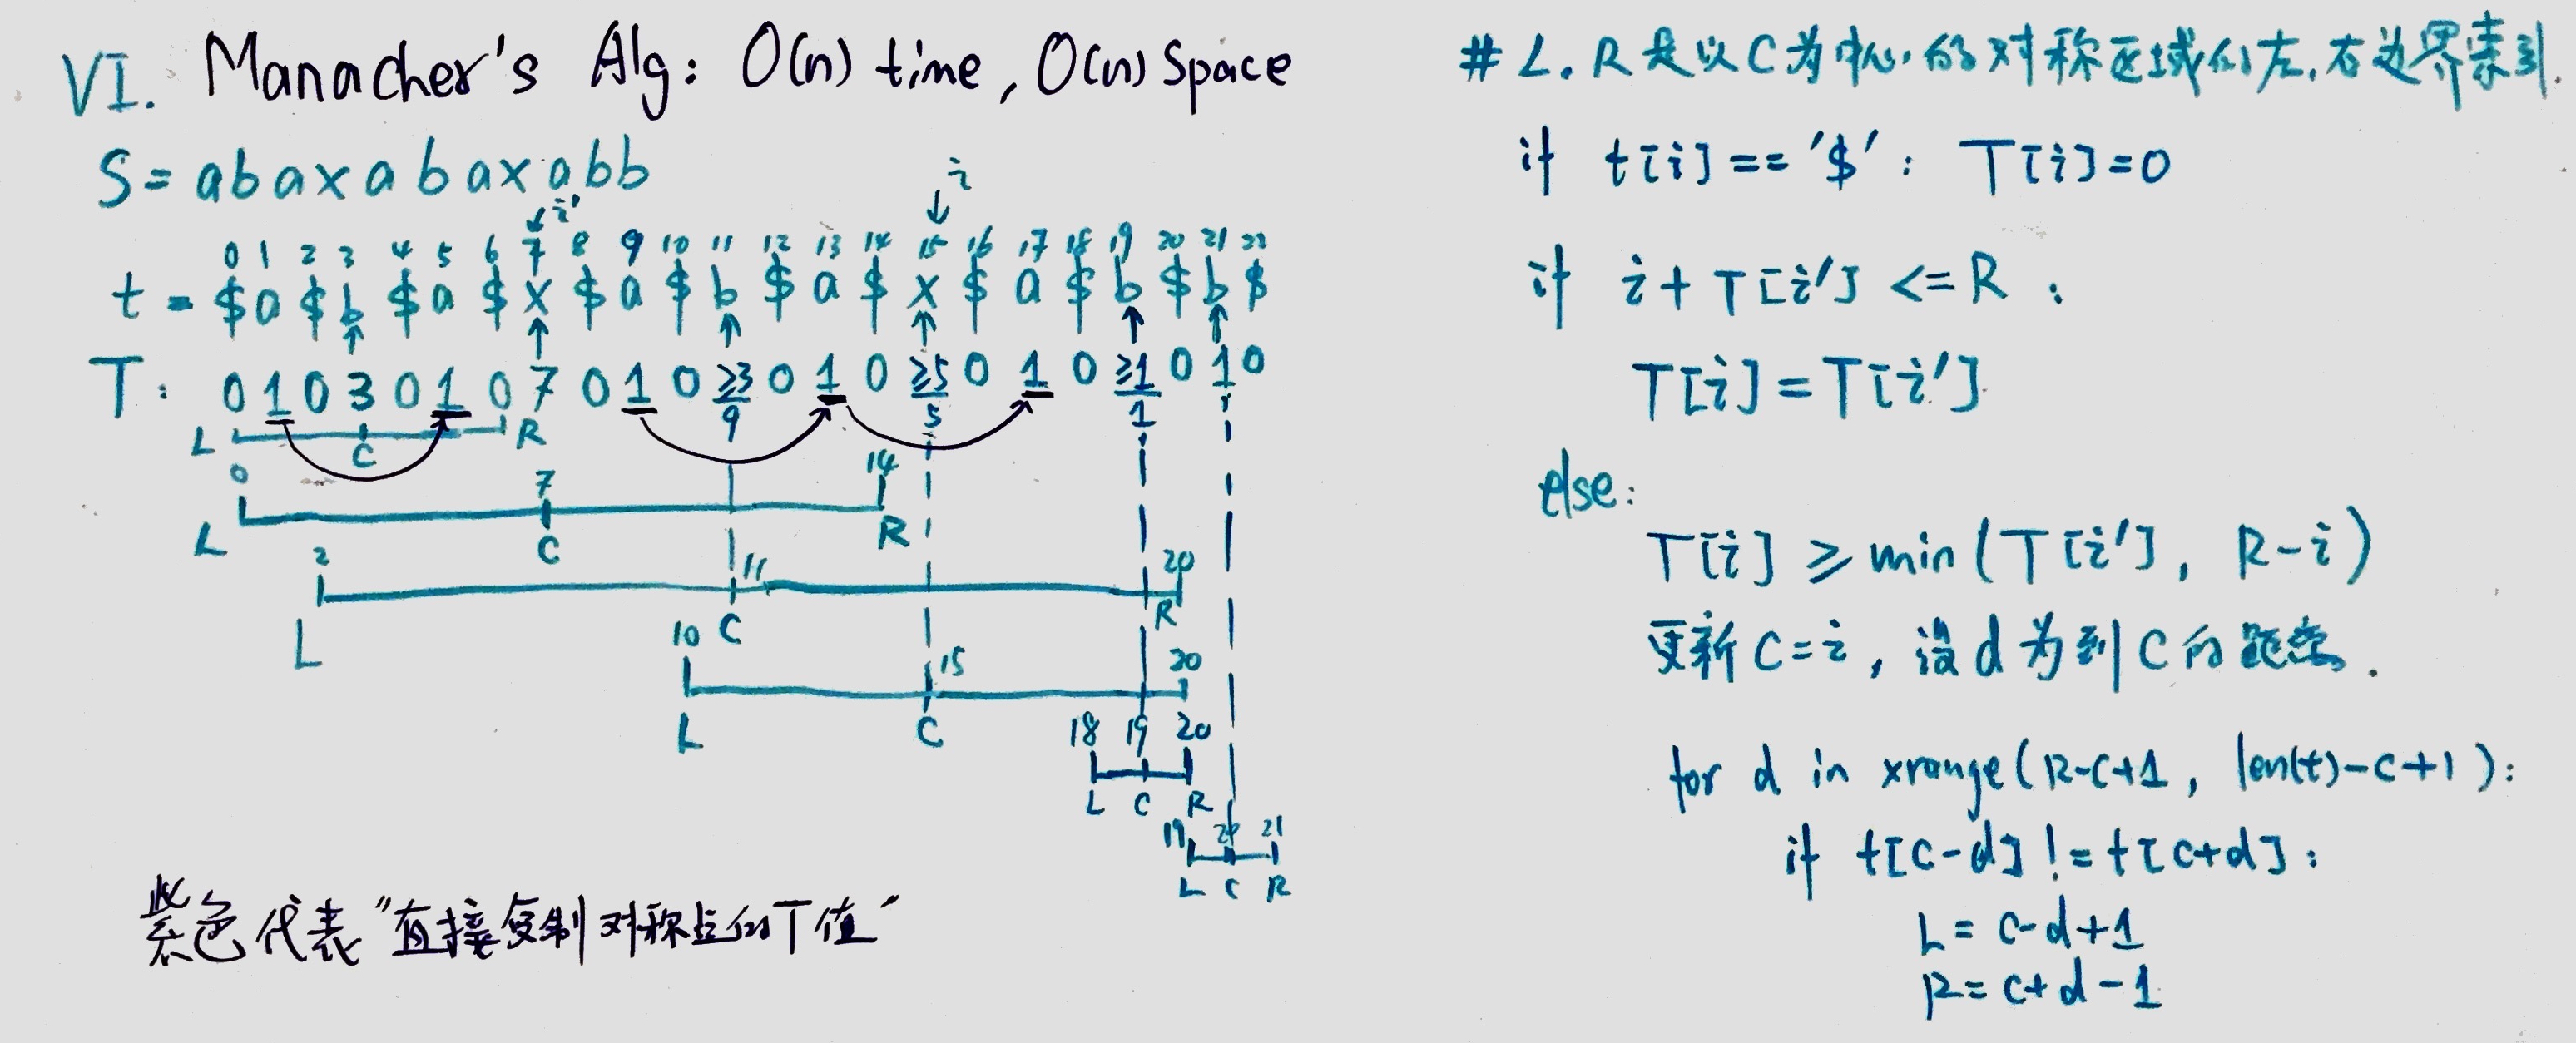
\includegraphics[width=\textwidth]{leetcode5-2.jpg}
    \centering \\
\end{figure}




\subsection{leetcode 13. Roman to Integer}
Given a roman numeral, convert it to an integer. Input is guaranteed to be within the range from 1 to 3999. \\

\begin{CJK*}{UTF8}{gbsn}
\noindent 解题思路:这类转换的题目,可以考虑建立一个字典,这样可以在$O(1)$的时间之内完成单个字符的转换。这道题的解题方法是从后向前遍历字符串:如果当前字符对应的数值不小于其后字符对应的数值,就进行累加;如果小于,则从累加和中减去其对应的数值。参见示例图。\\
\end{CJK*}

\begin{lstlisting}[language=Python, caption=Problem13. Roman to Integer]

class Solution(object):
    def romanToInt(self, s):  # O(n) time
        """
        :type s: str
        :rtype: int
        """
        n = len(s)
        dict = {'M':1000,'D':500,'C':100,'L':50,'X':10,'V':5,'I':1}
        result = dict[s[n-1]]
        for x in xrange(n-2, -1, -1):
            if dict[s[x]] >= dict[s[x+1]]:
                result += dict[s[x]]
            else:
                result -= dict[s[x]]
        return result
\end{lstlisting}

\begin{figure}[h]
    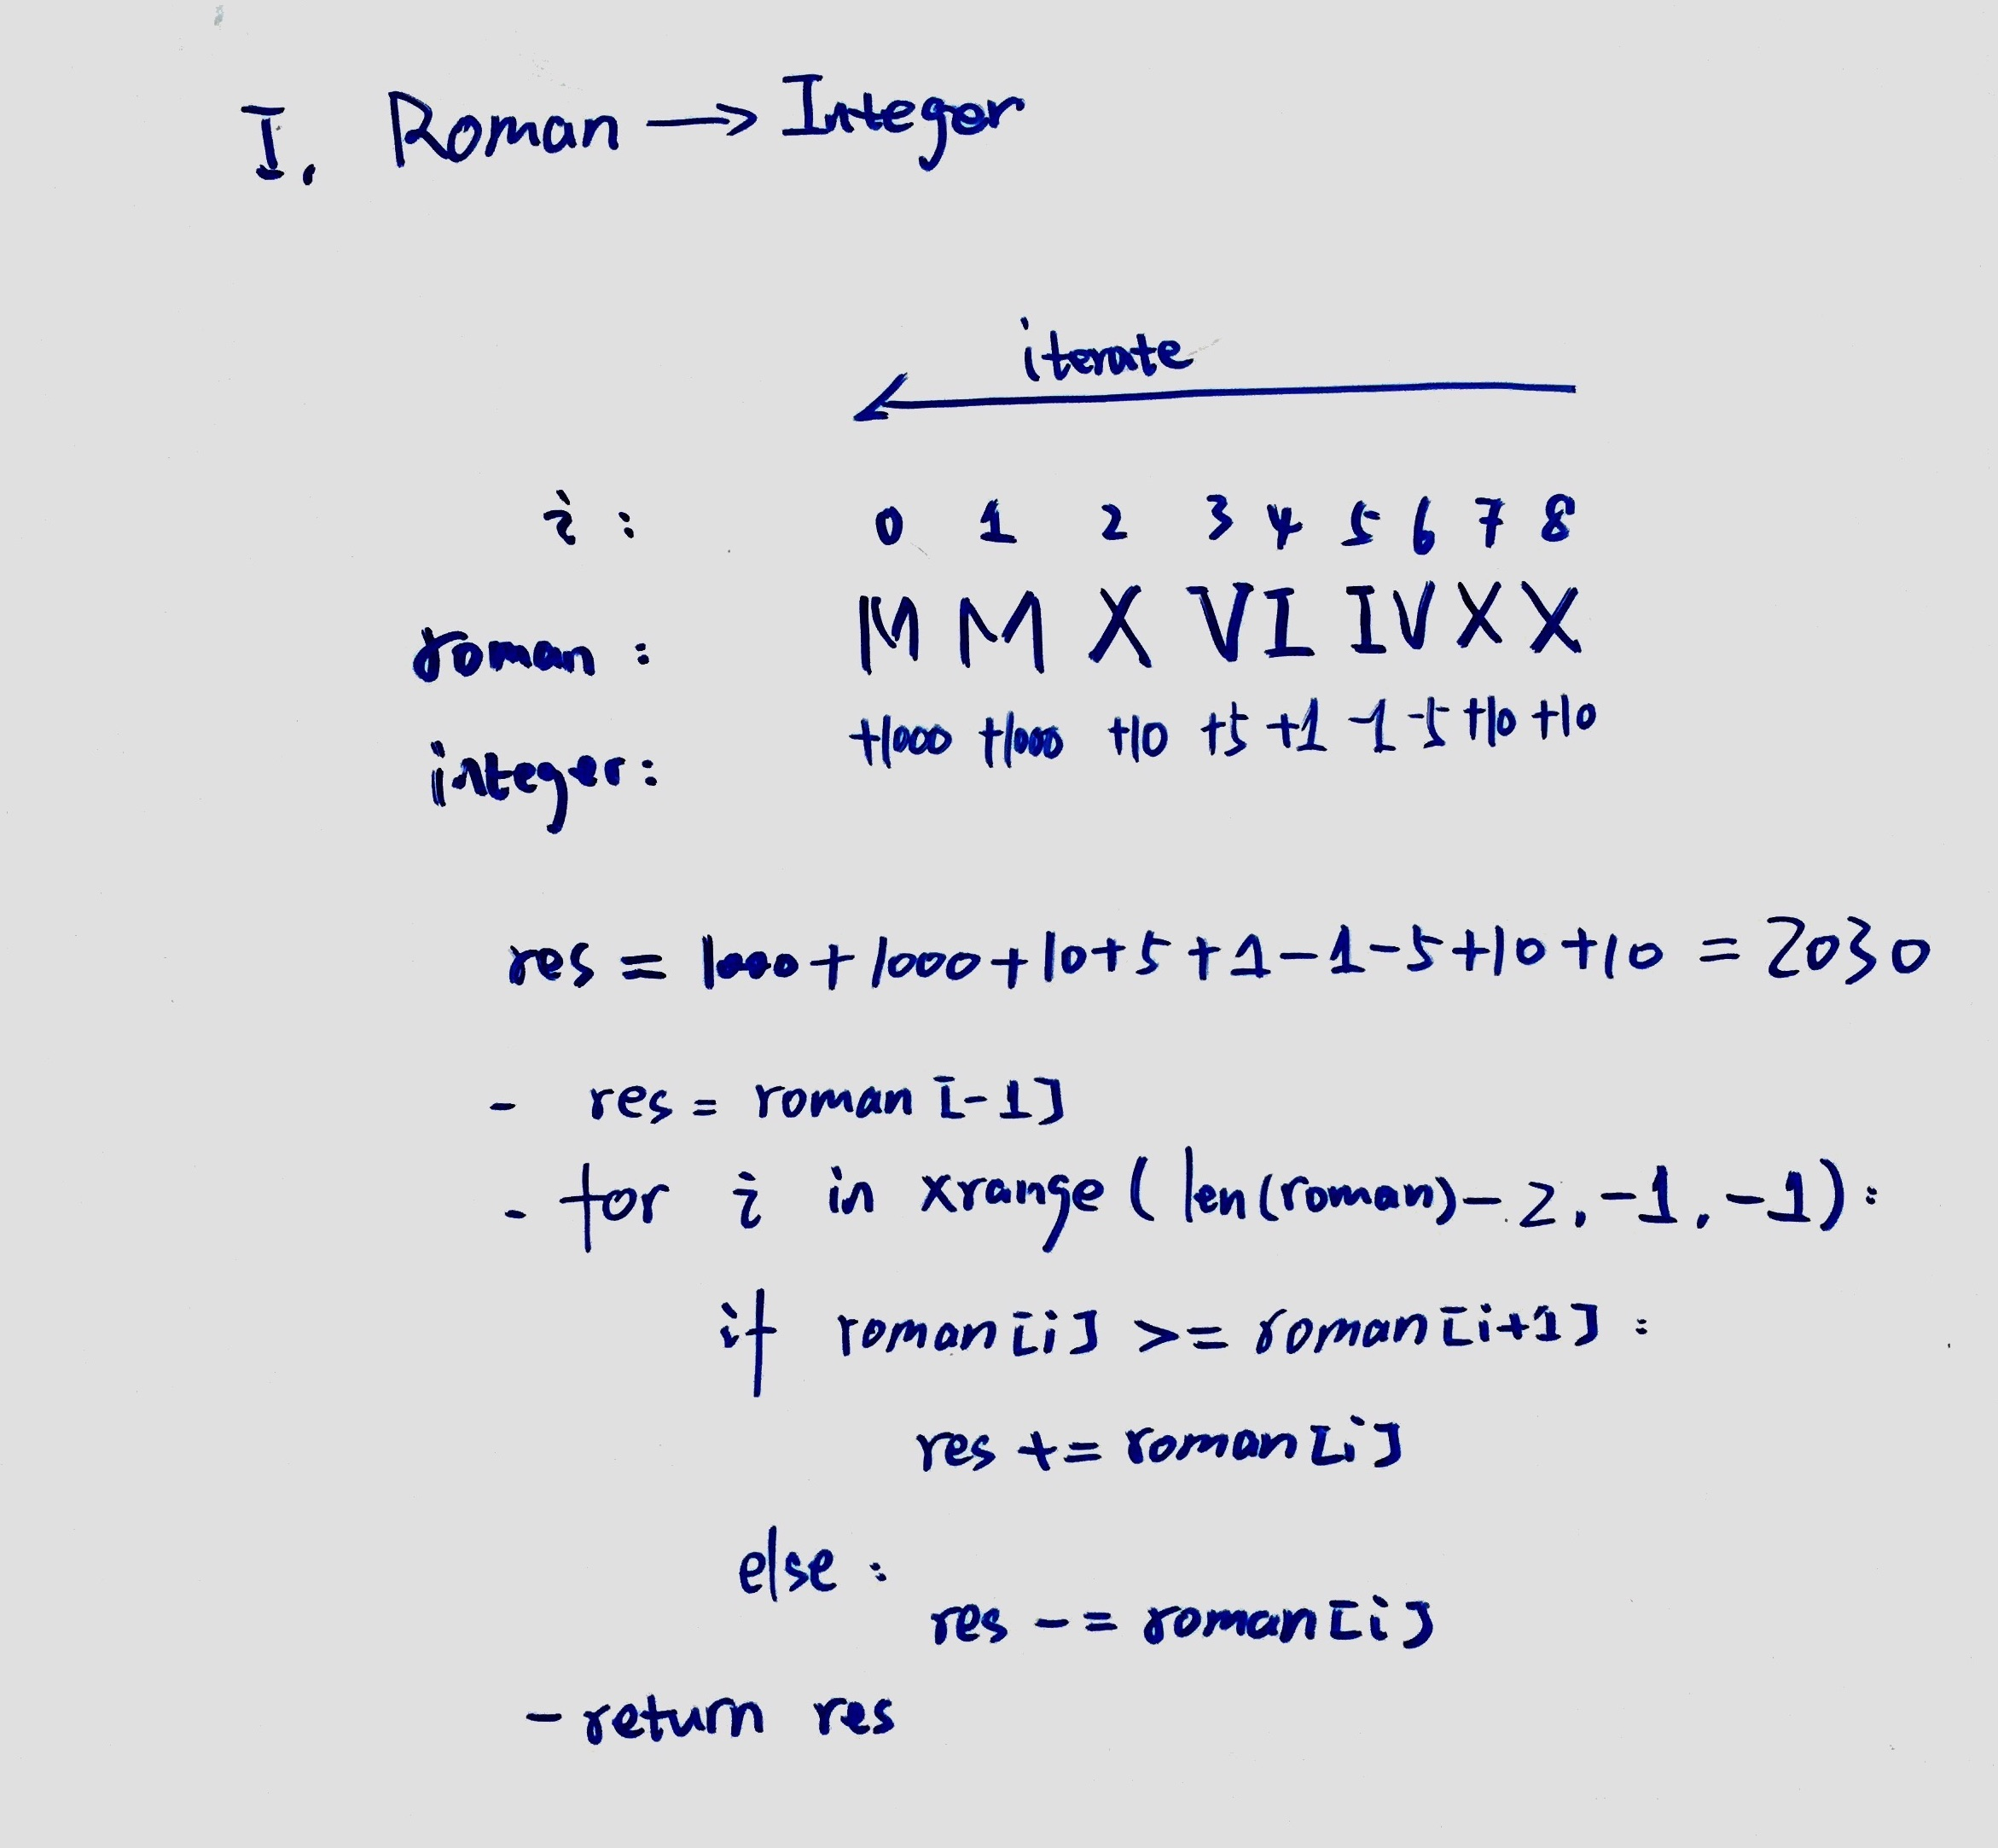
\includegraphics[width=10cm]{leetcode13.jpg}
    \centering\\
\end{figure}



\subsection{leetcode 12. Integer to Roman}
Given an integer, convert it to a roman numeral. Input is guaranteed to be within the range from 1 to 3999. \\

\begin{CJK*}{UTF8}{gbsn}
\noindent 解题思路:这道题比较简单,但是数据结构的选取上需要注意:因为要从1000开始,按照递减的次序,依次使用计量单位去除以num,因此在用Python编写算法时不能使用dict,因为dict.keys()生成的迭代器中key的次序并不是按照递减的次序排列,有可能是乱序,因此无法准确实现算法的设计目的。\\
\end{CJK*}

\begin{lstlisting}[language=Python, caption=Problem12. Integer to Roman]

class Solution(object):
    def intToRoman(self, num):
        """
        :type num: int
        :rtype: str
        """
        res = ''
        if num<=0: return res
        units =  [1000,900,500,400,100,90,50,40,10,9,5,4,1]
        romans = ['M','CM','D','CD','C','XC','L','XL','X','IX','V','IV','I']
        for i in xrange(len(units)):
            if num >= units[i]:
                count = num/units[i]
                num = num%units[i]
                res += romans[i]*count
        return res
\end{lstlisting}

\begin{figure}[h]
    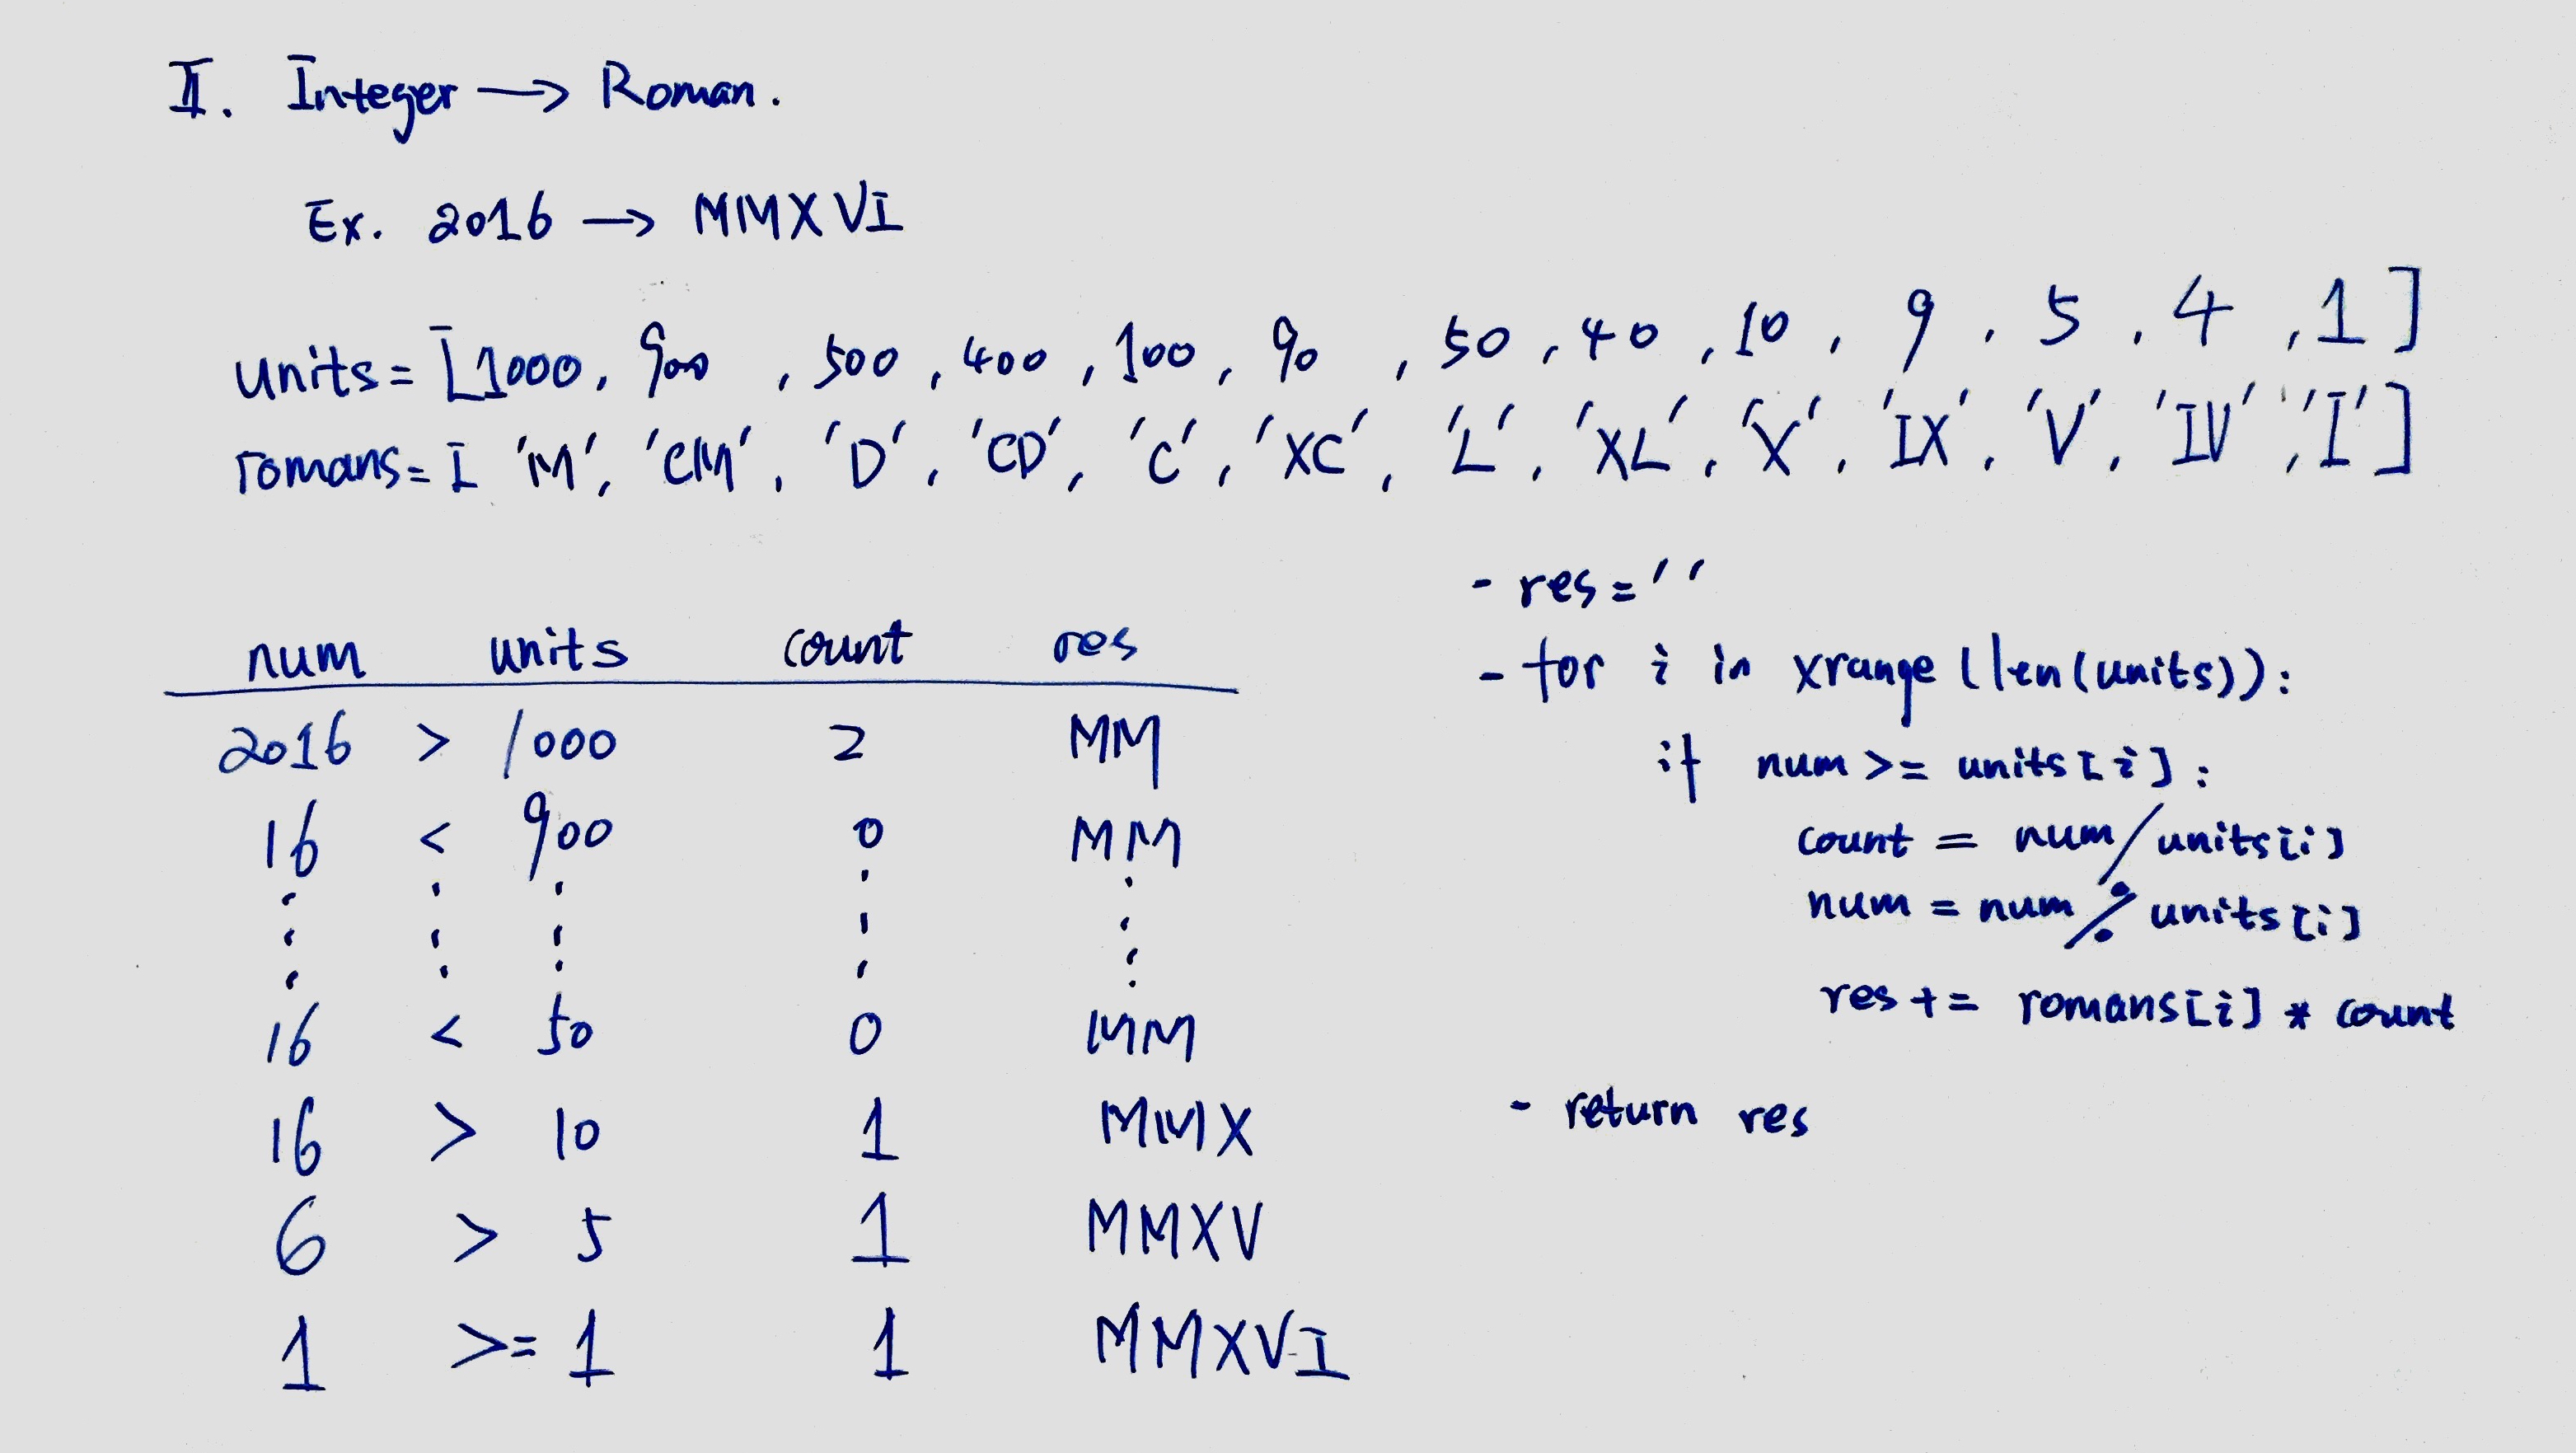
\includegraphics[width=\textwidth]{leetcode12.jpg}
    \centering\\
\end{figure}




\subsection{leetcode 44. Wildcard Matching}
Implement wildcard pattern matching with support for '?' and '*'. '?' Matches any single character. '*' Matches any sequence of characters (including the empty sequence). The matching should cover the entire input string (not partial).\\

\noindent The function prototype should be:
bool isMatch(const char *s, const char *p) \\

\noindent Some examples:
\begin{enumerate}
    \item isMatch("aa","a") $\to$ false
    \item isMatch("aa","aa") $\to$ true
    \item isMatch("aaa","aa") $\to$ false
    \item isMatch("aa", "*") $\to$ true
    \item isMatch("aa", "a*") $\to$ true
    \item isMatch("ab", "?*") $\to$ true
    \item isMatch("aab", "c*a*b") $\to$ false
\end{enumerate}

\begin{CJK*}{UTF8}{gbsn}
\noindent 该题目有3种解法:
\begin{enumerate}
    \item 递归算法:最直接的方法:依次进行比较$s$和$p$的每一个字符,同时考虑'*'和'?';在失配的情况下,用$s$的下一个字符和$p$的第一个字符重新开始比较。
    
    \item 动态归划算法:dp[i][j]表示s串前i个与p串前j个是否匹配。转换方程如下:
        \[ T[i][j] =
            \begin{cases}
                True        & \quad \text{if } i=0 \text{ and } j=0\\
                False       & \quad \text{if } i=0 \text{ or } j=0\\
                T[i-1][j-1] & \quad \text{if s[i] == p[j] or s[i] == '?'}\\
                False       & \quad \text{if s[i] != p[j]}\\
                T[i][j-1] \text{ or } T[i-1][j]  & \quad \text{if p[j]=='*'}\\
            \end{cases}
        \]
        
    \item 迭代算法:效率最高,只需要一次遍历。算法的关键在于,遇到“*”时,记录“*”的位置(lastCharMatchStar),同时记录字符串s的位置(lastCharMatchStar);然后继续用“*”后面一个字符仍然和s当前位置的字符比较;如果后续比较过程中出现不匹配的情况,则lastCharMatchStar+1,并从p的lastCharMatchStar+1位置和s的lastCharMatchStar位置重新开始比较。
\end{enumerate}
DP和迭代两种算法的分析和示例参见示例图一、二。
\end{CJK*}

\begin{figure}[h]
    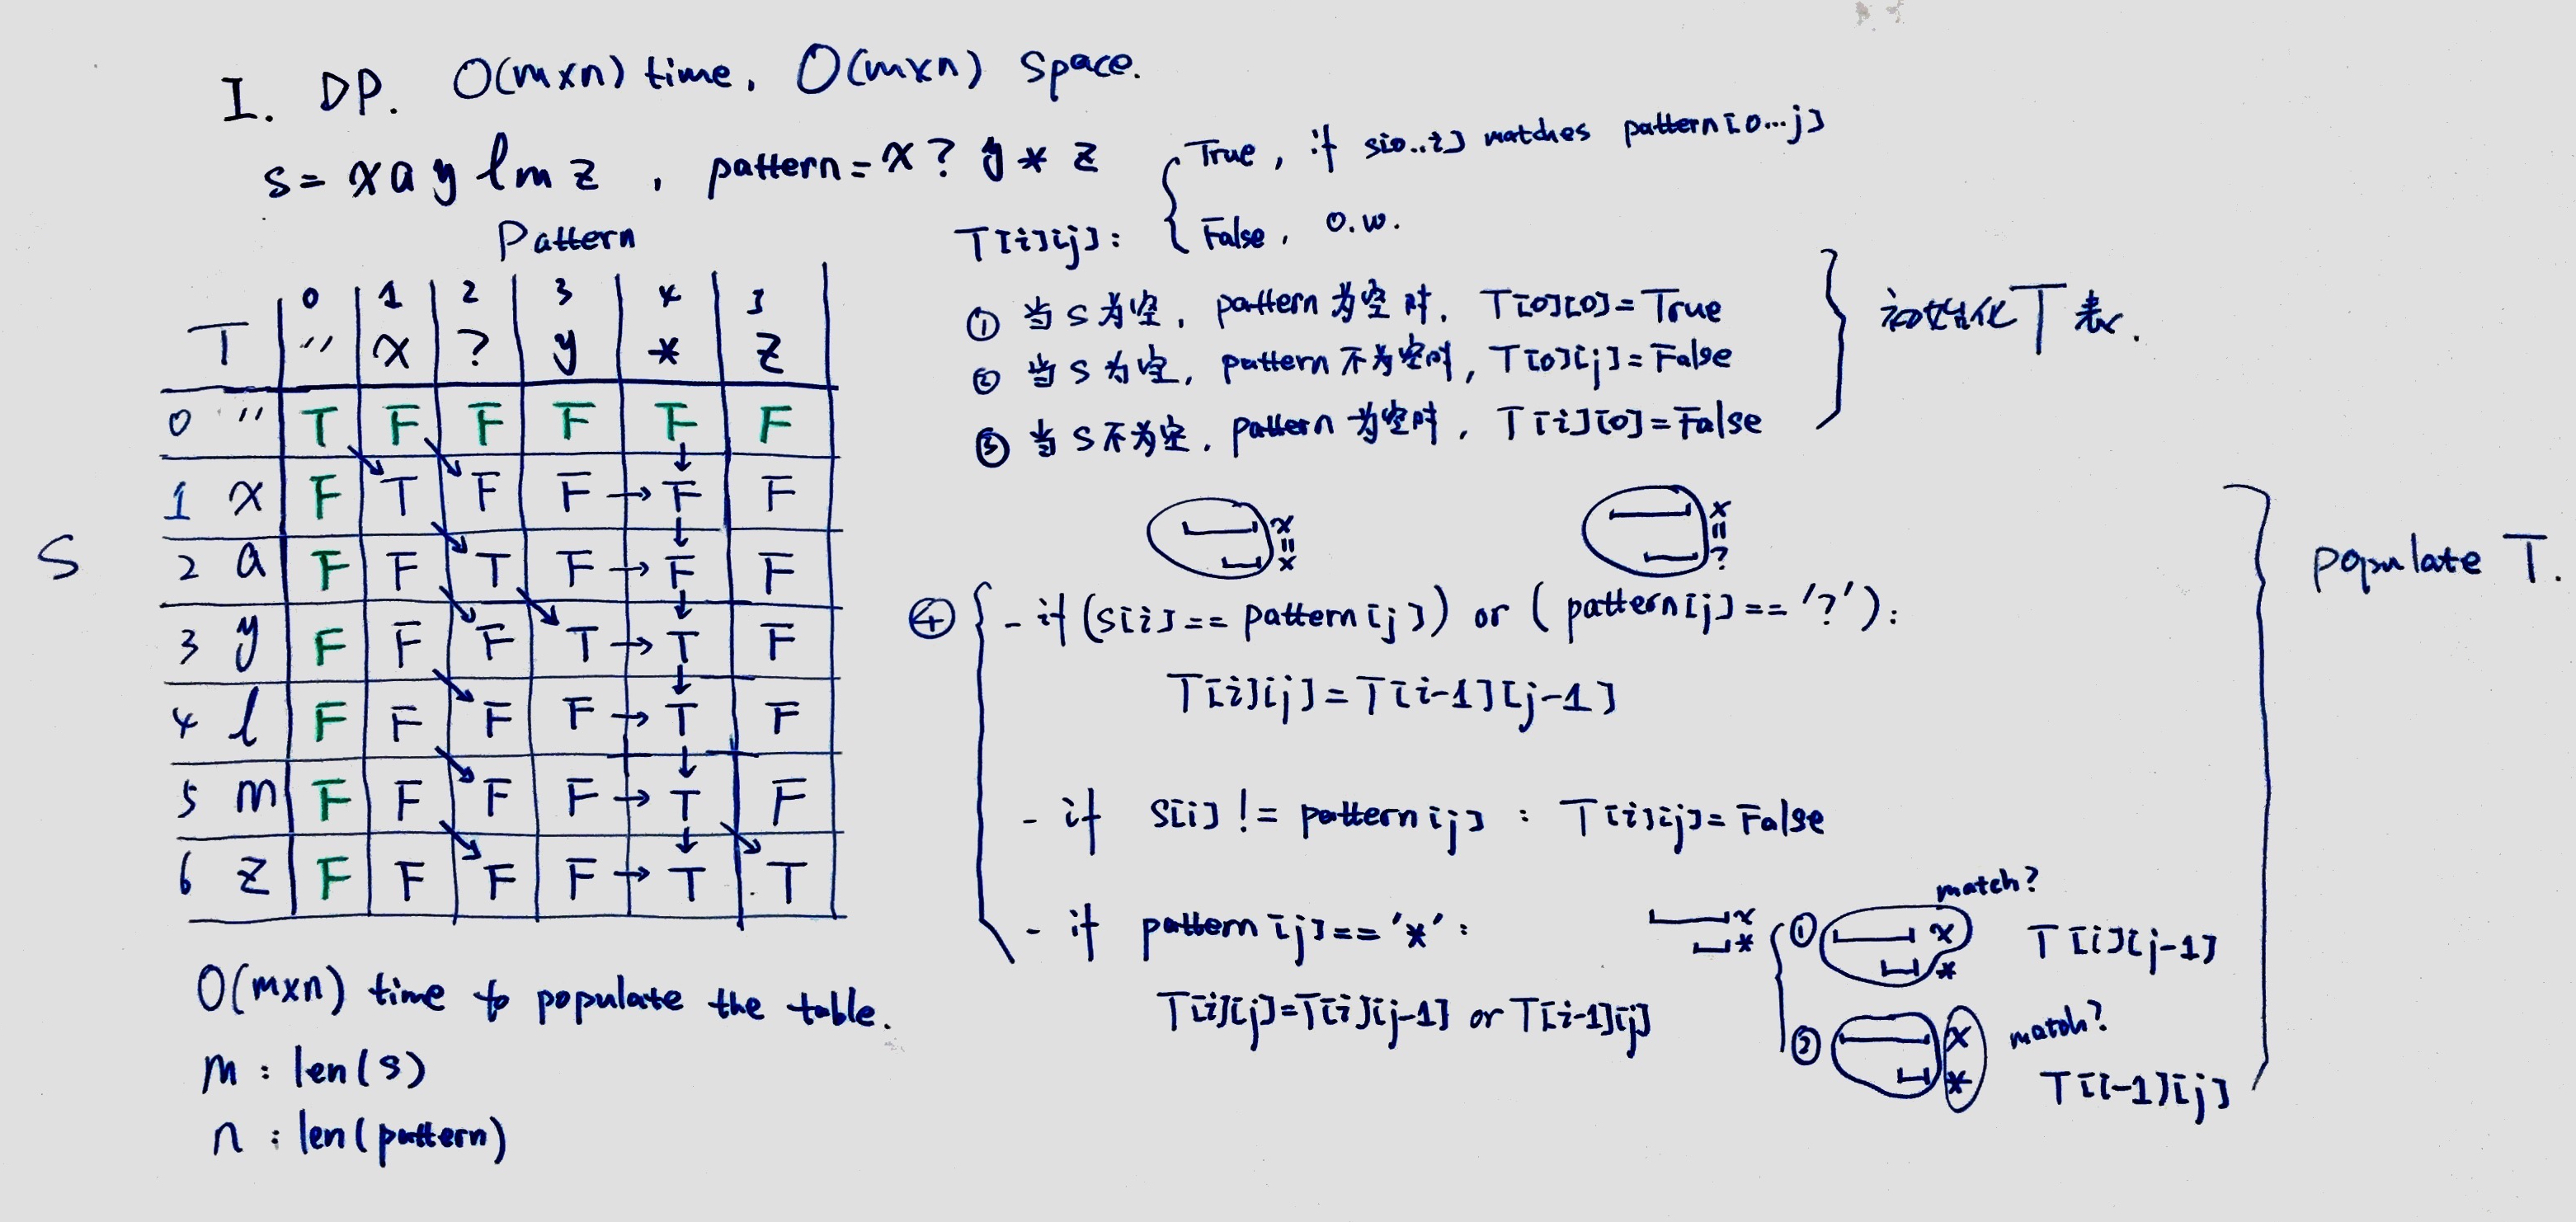
\includegraphics[width=\textwidth]{leetcode44-1.jpg}
    \centering
\end{figure}

\begin{figure}[h]
    \includegraphics[width=\textwidth]{leetcode44-2.jpg}
    \centering\\
\end{figure}

\begin{lstlisting}[language=Python, caption=Problem44. Wildcard Matching]

class Solution(object):
    def isMatch_recursive(self, s, p): # TLE error
        """
        :type s: str
        :type p: str
        :rtype: bool
        """
        if len(p)>len(s):
            return False
        elif len(s)==0 or len(p)==0:
            return len(s) == len(p)
        elif len(s)==1 and len(p)==1 and s==p:
            return True
        elif s[0]==p[0] or p[0]=='?':
            return self.isMatch(s[1:],p[1:])
        elif p[0]=='*':
            i = 0
            while i<len(p) and p[i]=='*':
                i += 1
            if i==len(p): return True
            j = 0
            while j<len(p) and not self.isMatch(s[j:], p[i:]):
                j += 1
            return j!=len(p)
        return False
        
    def isMatch_dp(self, s, p): # RT: O(n^2), Space: O(n^2)
        """
        :type s: str
        :type p: str
        :rtype: bool
        """
        if len(p) - p.count('*') > len(s): return False
        
        # replace multiple * with one *
        # e.g., a***b**c => a*b*c
        pattern = []
        isFirst = True
        for i in range(len(p)):
            if p[i]=='*':
                if isFirst:
                    pattern.append(p[i])
                    isFirst = False
            else:
                pattern.append(p[i])
                isFirst = True
        m, n = len(s), len(pattern)
        
        # initialize dp matrix
        dp=[[False for _ in range(n+1)] for _ in range(m+1)]
        dp[0][0]=True
        if n>0 and pattern[0]=='*': dp[0][1] = True
        
        # populate the dp matrix
        for i in range(1, m+1): # for string
            for j in range(1, n+1): # for pattern
                if pattern[j-1]=='*':
                    dp[i][j] = dp[i-1][j] or dp[i][j-1]
                elif s[i-1]==pattern[j-1] or pattern[j-1]=='?':
                    dp[i][j] = dp[i-1][j-1]
                else:
                    dp[i][j] = False
        return dp[m][n]

    def isMatch_iterative(self, s, p): # RT: O(n), Space: O(1)
        """
        :type s: str
        :type p: str
        :rtype: bool
        """
        # the position of the last occurrence of * in p
        lastStartPos = -1
        # the position of the last character in s which 
        # matches with *
        lastCharMatchStar = 0
        idxPattern = idxStr = 0
        while idxStr < len(s):
            # when there is a match, continue to compare 
            # the characters in s and p
            if idxPattern<len(p) and (s[idxStr]==p[idxPattern] or p[idxPattern]=='?'):
                idxStr += 1
                idxPattern += 1
                continue
            # when * comes, save the positions of idxPattern
            # and idxStr
            elif idxPattern<len(p) and p[idxPattern]=='*':
                lastStartPos = idxPattern
                lastCharMatchStar = idxStr
                idxPattern+=1
                continue
            # when there is a conflict, and we have a star, 
            # reset idxPattern to point to the next position 
            # of previous, and also move lastCharMatchStar 
            # to its next position, and set idxStr to point 
            # to lastCharMatchStar's position; 
            # after these settings, continue to check
            elif lastStartPos!=-1:
                idxPattern = lastStartPos+1
                lastCharMatchStar += 1
                idxStr = lastCharMatchStar
                continue
            # if all the conditions are not satisfied, 
            # s does not match p.
            else: return False
        while idxPattern<len(p) and p[idxPattern]=='*':
            idxPattern += 1
        if idxPattern == len(p): return True
        return False
\end{lstlisting}






%%%%%%%%%%%%%%%%%%%%%%%%%%%%%%%%%%%%%%%%%%%%%%%%%%%%%%%%%%%%%%%%%%%%%%%%
%%%%%%%%%%%%%%%%%%%%%%%%% Stack and Queue %%%%%%%%%%%%%%%%%%%%%%%%%%%%%%
%%%%%%%%%%%%%%%%%%%%%%%%%%%%%%%%%%%%%%%%%%%%%%%%%%%%%%%%%%%%%%%%%%%%%%%%


\section{Stack and Queue}

\subsection{Stack}
\subsubsection{leetcode 20. Valid Parentheses}
Given a string containing just the characters '(', ')', '\{', '\}', '[' and ']', determine if the input string is valid. The brackets must close in the correct order, "()" and "()[]\{\}" are all valid but "(]" and "([)]" are not. \\

\begin{CJK*}{UTF8}{gbsn}
\noindent 解题思路:这道题考查对栈数据结构的基本知识,问题比较简单。解题的基本步骤参考题图。
\end{CJK*}

\begin{figure}[h]
    \includegraphics[width=\textwidth]{leetcode20.jpg}
    \centering
\end{figure}

\begin{lstlisting}[language=Python, caption=Problem20. Valid Parentheses]

class Solution(object):
    def isValid(self, s):
        """
        :type s: str
        :rtype: bool
        """
        stack = []
        for x in s:
            if x in '([{': stack.append(x)
            else:
                if stack==[]: return False
                top = stack.pop()
                if (top=='(' and x==')') or \
                   (top=='[' and x==']') or \
                   (top=='{' and x=='}'):
                    continue
                else: return False
        if stack != []: return False
        return True
\end{lstlisting}



\subsubsection{leetcode 32. Longest Valid Parentheses}
Given a string containing just the characters '(' and ')', find the length of the longest valid (well-formed) parentheses substring. For "(()", the longest valid parentheses substring is "()", which has length = 2. Another example is ")()())", where the longest valid parentheses substring is "()()", which has length = 4. \\

\begin{CJK*}{UTF8}{gbsn}
\noindent 解题思路:这道题是个hard级别的题,解题思路与leetcode 20. Valid Parentheses有所差别,需要注意左括号多和右括号多这两种情况。
\end{CJK*}

\begin{figure}[h]
    \includegraphics[width=\textwidth]{leetcode32.jpg}
    \centering \\
\end{figure}

\begin{lstlisting}[language=Python, caption=Problem32. Longest Valid Parentheses]

class Solution(object):
    def longestValidParentheses(self, s): # RT: O(n), Space: O(n)
        """
        :type s: str
        :rtype: int
        """
        maxlen = 0

        # store the indices of all unmatched left brackets
        stack = []

        # index of the last unmatched right bracket
        last_unmatched_right_bracket = -1

        for i in range(len(s)):
            if s[i] == '(':
                stack.append(i)
            else:
                # if s[i] is ')'
                if stack == []:
                    last_unmatched_right_bracket = i
                else:
                    stack.pop()
                    if stack == []:
                        maxlen = max(maxlen, i - last_unmatched_right_bracket)
                    else:
                        maxlen = max(maxlen, i-stack[-1])
        return maxlen
\end{lstlisting}






\subsubsection{leetcode 84. Largest Rectangle in Histogram}
Given n non-negative integers representing the histogram's bar height where the width of each bar is 1, find the area of largest rectangle in the histogram. For example, given heights = [2,1,5,6,2,3], return 10. \\

\begin{CJK*}{UTF8}{gbsn}
\noindent 解题思路:在序列保持递增的时候,将当前索引入栈stack;如果序列的递增性在当前索引$x$处被破坏,那么就弹出栈顶的索引,直到栈顶索引对应的数值小于当前索引对应的数值。每次弹出的栈顶索引top,就计算一次形成的矩形的面积:矩形的高是height[top],矩形的宽是$x-stack[-1]-1$。注意:计算宽度的时候不能用$x-top$,因为如果索引top之前紧邻它的索引对应的数值比索引top对应的数值大的时候,这样计算的宽度就没有包含之前的部分。参考下面的示例图中的分析和演算过程。
\end{CJK*}

\begin{figure}[h]
    \includegraphics[width=\textwidth]{leetcode84.jpg}
    \centering \\
\end{figure}

\begin{lstlisting}[language=Python, caption=Problem84. Largest Rectangle in Histogram]

class Solution(object):
    def largestRectangleArea(self, heights): # RT: O(n), Space: O(n)
        """
        :type heights: List[int]
        :rtype: int
        """
        n = len(heights)
        maxarea, area = 0, 0
        stack = []
        x = 0
        while x < n:
            if stack==[] or (heights[stack[-1]] <= heights[x]):
                stack.append(x); x+=1
            else:
                top = stack.pop()
                if stack==[]:
                    area = heights[top] * x
                else:
                    area = heights[top] * (x-stack[-1]-1)
                maxarea = max(maxarea, area)
        while stack != []:
            top = stack.pop()
            if stack == []:
                area = heights[top] * x
            else:
                area = heights[top] * (x-stack[-1]-1)
            maxarea = max(maxarea, area)
        return maxarea
\end{lstlisting}




\subsubsection{leetcode 150. Evaluate Reverse Polish Notation}
Evaluate the value of an arithmetic expression in Reverse Polish Notation. Valid operators are +, -, *, /. Each operand may be an integer or another expression. \\

\noindent Some examples:
\begin{itemize}
    \item $["2", "1", "+", "3", "*"] \to ((2 + 1) * 3) \to 9$
    \item $["4", "13", "5", "/", "+"] \to (4 + (13 / 5)) \to 6$
\end{itemize}
  
\begin{CJK*}{UTF8}{gbsn}
\noindent 这道题对于Python实现有两个陷阱:第一个是栈的先进后出特性,在做减法和除法时,应该是后一个弹出的值作为被减数和被除数;第二个陷阱与Python版本相关,Python2.x的除法是floor division,所以在两个操作数异号时,得到的结果会有错,例如-3/2=-2,而不是-1;解决的办法是先判断一下两个操作数是否同号,如果是一正一负,那么就先转换成相应的正数,然后做完除法以后将结果置为负值即可(参考代码行21-22)。
\end{CJK*}

\begin{lstlisting}[language=Python, caption=Problem150. Evaluate Reverse Polish Notation]

class Solution(object):
    def evalRPN(self, tokens):
        """
        :type tokens: List[str]
        :rtype: int
        """
        stack = []
        for x in tokens:
            if stack==[] or x not in '+-*/':
                stack.append(int(x))
            else:
                op1, op2 = stack.pop(), stack.pop()
                if x=='+': stack.append(op1+op2)
                elif x=='-': stack.append(op2-op1)
                elif x=='*': stack.append(op1*op2)
                elif x=='/':
                    # Python2 uses "floor division"
                    # e.g., -1/2=-1, but not 0
                    if op1*op2 < 0:
                        stack.append(-(-op2/op1))
                    else: stack.append(op2/op1)
        return stack.pop()
\end{lstlisting}



%%%%%%%%%%%%%%%%%%%%%%%%%%%%%%%%%%%%%%%%%%%%%%%%%%%%%%%%%%%%%%%%%%%
%%%%%%%%% Trees %%%%%%%%%%%%%%%%%%%%%%%%%%%%%%%%%%%%%%%%%%%%%%%%%%%
%%%%%%%%%%%%%%%%%%%%%%%%%%%%%%%%%%%%%%%%%%%%%%%%%%%%%%%%%%%%%%%%%%%

\section{Trees}

\subsection{Summary}
\begin{CJK*}{UTF8}{gbsn}
\noindent 有关树的考点:
\begin{enumerate}
    \item 第一类问题是树的先序、中序、后序遍历算法的递归和迭代实现,重点是迭代。很多题目的算法都是基于改进上述三种遍历算法而得到的。需要注意,后序遍历的迭代算法需要一些小技巧。有关二叉树的三种遍历算法见leetcode 144, 94, 145题的解法。
    
    \item 第二类问题源自于第一类问题,主要考查的是对于先序、中序、后序遍历算法得出的结果的理解,比如中序遍历BST二叉搜索数得到的序列是递增序列,题目leetcode 99就是通过这个性质来构造算法。
    
    \item 第三类问题是给出二叉树的先序和中序(或者后序和中序),然后构造二叉树。这里需要注意只有先序和后序是无法构造二叉树的,因为无法确定根的位置。leetcode105、106考查了这个知识点。
    
    \item 第四类问题关于树的结构性的问题。这类问题主要是考查对二叉树的深度和广度两种优先搜索算法的理解。比如leetcode 100、101、102、103、107等等题目都是基于上述两种基本算法的改进而得。其中,广度优先搜索算法是重点。
    
    \item 第五类问题是关于树的分支、路径、深度、高度等属性。这类问题考查的实质就是对于树的DFS算法的熟悉和掌握程度。通常用DFS的递归实现即可。
\end{enumerate}\\
\end{CJK*}

\subsection{Binary Tree Traversal}
\subsubsection{leetcode 105. Construct Binary Tree from Preorder and Inorder Traversal}
Given preorder and inorder traversal of a tree, construct the binary tree. Note: You may assume that duplicates do not exist in the tree. \\

\begin{CJK*}{UTF8}{gbsn}
\noindent 解题思路:二叉树的先序遍历提供了树根的位置,即先序遍历的第一个元素;在确定了树根在中序遍历中的位置以后,中序遍历提供左、右子树的信息。据此,可以递归构造二叉树。这里的关键点是第21行代码,在每次确定树根以后,需要删除先序遍历中的树根值,以缩小先序遍历的长度,否则代码会造成memory limit exceeded错误。参考下面的示例图中的分析。参考下面示例图中的分析和演算。\\
\end{CJK*}

\begin{lstlisting}[language=Python, caption=Problem105. Construct Binary Tree from Preorder and Inorder Traversal]

# Definition for a binary tree node.
# class TreeNode(object):
#     def __init__(self, x):
#         self.val = x
#         self.left = None
#         self.right = None

class Solution(object):
    def buildTree(self, preorder, inorder):
        """
        :type preorder: List[int]
        :type inorder: List[int]
        :rtype: TreeNode
        """
        if len(preorder) == 0 or len(inorder)==0:
            return None
    
        root = TreeNode(preorder[0])
        i = inorder.index(root.val)
        preorder.pop(0)
        root.left = self.buildTree(preorder,inorder[:i])
        root.right = self.buildTree(preorder,inorder[i+1:])
        
        return root
\end{lstlisting}

\begin{figure}[h]
    \includegraphics[width=\textwidth]{leetcode105.jpg}
    \centering \\
\end{figure}


\subsubsection{leetcode 106. Construct Binary Tree from Inorder and Postorder Traversal}
Given inorder and postorder traversal of a tree, construct the binary tree.  Note: You may assume that duplicates do not exist in the tree. \\

\begin{CJK*}{UTF8}{gbsn}
\noindent 解题思路:与leetcode 105类似的方法。不同之处在于,本题由后序遍历提供了树根的位置信息,即后序遍历的最后一个元素即为树根;在确定了树根在中序遍历中的位置以后,中序遍历提供左、右子树的信息。据此,可以递归构造二叉树。这里的关键点是第21行代码,在每次确定树根以后,需要删除先序遍历中的树根值,以缩小先序遍历的长度,否则代码会造成memory limit exceeded错误。参考下面示例图中的分析和演算。\\
\end{CJK*}

\begin{lstlisting}[language=Python, caption=Problem106. Construct Binary Tree from Inorder and Postorder Traversal]

# Definition for a binary tree node.
# class TreeNode(object):
#     def __init__(self, x):
#         self.val = x
#         self.left = None
#         self.right = None

class Solution(object):
    def buildTree(self, inorder, postorder): # MLE error
        """
        :type inorder: List[int]
        :type postorder: List[int]
        :rtype: TreeNode
        """
        if len(inorder)==0 or len(postorder)==0:
            return None
        root = TreeNode(postorder[-1])
        i = inorder.index(root.val)
        postorder.pop()
        root.right = self.buildTree(inorder[i+1:], postorder)
        root.left = self.buildTree(inorder[:i], postorder)
        
        return root
\end{lstlisting}

\begin{figure}[h]
    \includegraphics[width=\textwidth]{leetcode106.jpg}
    \centering \\
\end{figure}


\subsubsection{leetcode 144. Binary Tree Preorder Traversal}
Given a binary tree, return the preorder traversal of its nodes' values. Note: Recursive solution is trivial, could you do it iteratively? \\

\begin{CJK*}{UTF8}{gbsn}
\noindent 解题思路:在使用栈来存放结点的时候,要先放右子树的根结点,再放左子树的根结点。参考下面示例图中的分析和演算。\\
\end{CJK*}

\begin{lstlisting}[language=Python, caption=Problem144. Binary Tree Preorder Traversal]

# Definition for a binary tree node.
# class TreeNode(object):
#     def __init__(self, x):
#         self.val = x
#         self.left = None
#         self.right = None

class Solution(object):
    def preorderTraversal_iterative(self, root):  # O(n) time, O(n) space
        """
        :type root: TreeNode
        :rtype: List[int]
        """
        res = []
        if root == None:
            return res
        stack = [root]
        while stack != []:
            node = stack.pop()
            res += [node.val]
            if node.right is not None:
                stack.append(node.right)
            if node.left is not None:
                stack.append(node.left)
        return res

    def preorderTraversal_recursive(self, root):  # O(n) time
        """
        :type root: TreeNode
        :rtype: List[int]
        """
        res = []
        if root == None: return res
        # root
        res += [root.val]
        # left subtree
        if root.left is not None:
            res += self.preorderTraversal_recursive(root.left)
        # right subtree
        if root.right is not None:
            res += self.preorderTraversal_recursive(root.right)

        return res
\end{lstlisting}

\begin{figure}[h]
    \includegraphics[width=\textwidth]{leetcode144.jpg}
    \centering \\
\end{figure}





\subsubsection{leetcode 94. Binary Tree Inorder Traversal}
Given a binary tree, return the inorder traversal of its nodes' values. Note: Recursive solution is trivial, could you do it iteratively? \\

\begin{lstlisting}[language=Python, caption=Problem94. Binary Tree Inorder Traversal]

# Definition for a binary tree node.
# class TreeNode(object):
#     def __init__(self, x):
#         self.val = x
#         self.left = None
#         self.right = None

class Solution(object):
    def inorderTraversal_iterative(self, root):
        """
        :type root: TreeNode
        :rtype: List[int]
        """
        res = []
        if root is None:
            return res

        stack = []
        while len(stack) > 0 or root:
            if root:
                stack.append(root)
                root = root.left
            else:
                root = stack.pop()
                res.append(root.val)
                root = root.right
        return res

    def inorderTraversal_recursive(self, root):
        """
        :type root: TreeNode
        :rtype: List[int]
        """
        res = []
        if root:
            return res

        # traverse left subtree
        if root.left:
            res += self.inorderTraversal_recursive(root.left)

        # visit root
        res.append(root.val)

        # traverse right subtree
        if root.right:
            res += self.inorderTraversal_recursive(root.right)

        return res
\end{lstlisting}



\subsubsection{leetcode 145. Binary Tree Postorder Traversal}
Given a binary tree, return the postorder traversal of its nodes' values. Note: Recursive solution is trivial, could you do it iteratively? \\

\begin{lstlisting}[language=Python, caption=Problem145. Binary Tree Postorder Traversal]

# Definition for a binary tree node.
# class TreeNode(object):
#     def __init__(self, x):
#         self.val = x
#         self.left = None
#         self.right = None

class Solution(object):
    def postorderTraversal_iterative(self, root):
        """
        :type root: TreeNode
        :rtype: List[int]
        """
        res = []
        if root is None:
            return res

        pre = None
        stack = [root]
        while len(stack) > 0:
            curr = stack[-1]
            if (curr.left is None and curr.right is None) or (pre and (pre == curr.left or pre == curr.right)):
                res.append(curr.val)
                pre = stack.pop()
            else:
                if curr.right:
                    stack.append(curr.right)
                if curr.left:
                    stack.append(curr.left)
        return res

    def postorderTraversal_recursive(self, root):
        """
        :type root: TreeNode
        :rtype: List[int]
        """
        res = []
        if root is None:
            return res

        if root.left:
            res += self.postorderTraversal_recursive(root.left)
        if root.right:
            res += self.postorderTraversal_recursive(root.right)
            
        res.append(root.val)
        return res
\end{lstlisting}



\subsubsection{leetcode 102. Binary Tree Level Order Traversal}
Given a binary tree, return the level order traversal of its nodes' values. (ie, from left to right, level by level). \\

\begin{lstlisting}[language=Python, caption=Problem102. Binary Tree Level Order Traversal]

# Definition for a binary tree node.
# class TreeNode(object):
#     def __init__(self, x):
#         self.val = x
#         self.left = None
#         self.right = None

class Solution(object):
    def levelOrder(self, root):
        """
        :type root: TreeNode
        :rtype: List[List[int]]
        """
        res = []
        if root is None:
            return res
        currLevel = [root]
        while len(currLevel) > 0:
            nextLevel = []
            values = []
            for elem in currLevel:
                values.append(elem.val)
                if elem.left:
                    nextLevel.append(elem.left)
                if elem.right:
                    nextLevel.append(elem.right)
            if len(values) > 0:
                res.append(values)
            currLevel = nextLevel
        return res
\end{lstlisting}



\subsubsection{leetcode 107. Binary Tree Level Order Traversal II}
Given a binary tree, return the bottom-up level order traversal of its nodes' values. (ie, from left to right, level by level from leaf to root). \\

\noindent For example: Given binary tree $\{3,9,20,\#,\#,15,7\}$, return its bottom-up level order traversal as $ [[15,7],[9,20],[3]] $. \\

\begin{lstlisting}[language=Python, caption=Problem107. Binary Tree Level Order Traversal II]

# Definition for a binary tree node.
# class TreeNode(object):
#     def __init__(self, x):
#         self.val = x
#         self.left = None
#         self.right = None

class Solution(object):
    def levelOrderBottom(self, root):
        """
        :type root: TreeNode
        :rtype: List[List[int]]
        """
        res = []
        if root is None:
            return res
        currLevel = [root]
        while len(currLevel) > 0:
            nextLevel = []
            values = []
            for item in currLevel:
                values.append(item.val)
                if item.left: 
                    nextLevel.append(item.left)
                if item.right: 
                    nextLevel.append(item.right)
            if len(values) > 0: 
                res.append(values)
            currLevel = nextLevel
        return res[::-1]
\end{lstlisting}


\subsubsection{leetcode 103. Binary Tree Zigzag Level Order Traversal}
Given a binary tree, return the zigzag level order traversal of its nodes' values. (ie, from left to right, then right to left for the next level and alternate between). \\

\noindent For example: Given binary tree {3,9,20,#,#,15,7}, return its bottom-up level order traversal as $ [[3],[20,9],[15,7]] $. \\

\begin{CJK*}{UTF8}{gbsn}
\noindent 这道题与leetcode102类似,按照层来遍历二叉树。注意,这道题不要翻转结点列表,而是翻转每次得到的值列表,这样算法比较简单!
\end{CJK*}

\begin{figure}[h]
    \includegraphics[width=\textwidth]{leetcode103.jpg}
    \centering \\
\end{figure}

\begin{lstlisting}[language=Python, caption=Problem103. Binary Tree Zigzag Level Order Traversal]

# Definition for a binary tree node.
# class TreeNode(object):
#     def __init__(self, x):
#         self.val = x
#         self.left = None
#         self.right = None

class Solution(object):
    def zigzagLevelOrder(self, root):
        """
        :type root: TreeNode
        :rtype: List[List[int]]
        """
        res = []
        if root is None:
            return res
        currLevel = [root]
        reversed = False
        while len(currLevel) > 0:
            nextLevel = []
            values = []
            for item in currLevel:
                values.append(item.val)
                if item.left:
                    nextLevel.append(item.left)
                if item.right:
                    nextLevel.append(item.right)
            if len(values) > 0:
                res.append(values[::-1] if reversed else values)
            reversed = not reversed
            currLevel = nextLevel
        return res
\end{lstlisting}


\subsubsection{leetcode 100. Same Tree}
Given two binary trees, write a function to check if they are equal or not. Two binary trees are considered equal if they are \textbf{structurally identical} and the nodes have the \textbf{same value}. \\

\begin{CJK*}{UTF8}{gbsn}
\noindent 解题方法:参考示例图中的分析和代码。\\
\end{CJK*}

\begin{lstlisting}[language=Python, caption=Problem100. Same Tree]

# Definition for a binary tree node.
# class TreeNode(object):
#     def __init__(self, x):
#         self.val = x
#         self.left = None
#         self.right = None

class Solution(object):
    def isSameTree_iterative(self, p, q):
        """
        :type p: TreeNode
        :type q: TreeNode
        :rtype: bool
        """
        if p is None: 
            return q is None
        if q is None: 
            return p is None
        stack = [(p,q)]
        while len(stack) > 0:
            root1, root2 = stack.pop()
            if root1 is None and root2 is None: 
                continue
            elif root1 and root2 and root1.val == root2.val:
                stack.append((root1.left, root2.left))
                stack.append((root1.right, root2.right))
            else: 
                return False
        return True
        
    def isSameTree_recursive(self, p, q):
        """
        :type p: TreeNode
        :type q: TreeNode
        :rtype: bool
        """
        if p is None: 
            return q is None
        if q is None: 
            return False
        if p.val == q.val:
            return self.isSameTree_recursive(p.left, q.left) and self.isSameTree_recursive(p.right, q.right)
        else:
            return False
\end{lstlisting}

\begin{figure}[h]
    \includegraphics[width=\textwidth]{leetcode100.jpg}
    \centering \\
\end{figure}




\subsubsection{leetcode 101. Symmetric Tree}
Given a binary tree, check whether it is a mirror of itself (ie, symmetric around its center). Note: Bonus points if you could solve it both recursively and iteratively.\\

\begin{CJK*}{UTF8}{gbsn}
\noindent 解题方法:验证树的结构性问题,考查的重点是对二叉树遍历算法的理解。参考示例图中的分析和代码。
\end{CJK*}

\begin{figure}[h]
    \includegraphics[width=\textwidth]{leetcode101.jpg}
    \centering \\
\end{figure}


\begin{lstlisting}[language=Python, caption=Problem101. Symmetric Tree]

# Definition for a binary tree node.
# class TreeNode(object):
#     def __init__(self, x):
#         self.val = x
#         self.left = None
#         self.right = None

class Solution(object):
    def isSymmetric_iterative(self, root):
        if root is None:
            return True

        lqueue = [root.left]
        rqueue = [root.right]
        while len(lqueue) > 0 and len(rqueue) > 0:
            root1, root2 = lqueue.pop(0), rqueue.pop(0)
            if root1 is None and root2 is None:
                continue
            elif root1 and root2 and root1.val == root2.val:
                lqueue.append(root1.left)
                rqueue.append(root2.right)

                lqueue.append(root1.right)
                rqueue.append(root2.left)
            else:
                return False
        return True

    def isSymmetric_recursive(self, root):
        """
        :type root: TreeNode
        :rtype: bool
        """
        def checkSymmetry(root1, root2):
            if root1 is None: 
                return root2 is None
            if root2 is None:
                return False
            if root1.val == root2.val:
                return checkSymmetry(root1.left, root2.right) and checkSymmetry(root1.right, root2.left)
            else:
                return False

        if root is None:
            return True
        return checkSymmetry(root.left, root.right)
\end{lstlisting}


\subsubsection{leetcode 110. Balanced Binary Tree}
Given a binary tree, determine if it is height-balanced. For this problem, a height-balanced binary tree is defined as a binary tree in which the depth of the two subtrees of every node never differ by more than 1.\\

\begin{CJK*}{UTF8}{gbsn}
\noindent 解题方法:考查平衡二叉树的基本性质。参考示例图中的分析和代码。
\end{CJK*}

\begin{figure}[h]
    \includegraphics[width=\textwidth]{leetcode110.jpg}
    \centering \\
\end{figure}

\begin{lstlisting}[language=Python, caption=Problem110. Balanced Binary Tree]

# Definition for a binary tree node.
# class TreeNode(object):
#     def __init__(self, x):
#         self.val = x
#         self.left = None
#         self.right = None

class Solution(object):
    def isBalanced(self, root):
        def helper(root):
            if root is None:
                return True, 0

            # check left subtree
            left = helper(root.left)
            if left[0] == False:
                return False, -1

            # check right subtree
            right = helper(root.right)
            if right[0] == False:
                return False, -1

            # check if the depths of the two subtrees
            # differ by more than 1
            if abs(left[1]-right[1]) <= 1:
                return True, 1+max(left[1], right[1])
            else:
                return False, -1
        return helper(root)[0]
\end{lstlisting}





\subsubsection{leetcode 114. Flatten Binary Tree to Linked List}
Given a binary tree, flatten it to a linked list in-place. \\

\begin{CJK*}{UTF8}{gbsn}
\noindent 解题方法:这道题考查的基本点还是对于树的遍历算法的理解和掌握。观察题目给出的例子(参考下面示例图中的例子)可以发现:结果中的结点序列实际上就是二叉树的先序遍历的结果,所以考查点实际就是对二叉树先序遍历的掌握。如果不借助额外的存储,算法可以考虑使用递归实现。参考示例图中的分析和代码。
\end{CJK*}

\begin{figure}[h]
    \includegraphics[width=\textwidth]{leetcode114.jpg}
    \centering \\
\end{figure}

\begin{lstlisting}[language=Python, caption=Problem114. Flatten Binary Tree to Linked List]

# Definition for a binary tree node.
# class TreeNode(object):
#     def __init__(self, x):
#         self.val = x
#         self.left = None
#         self.right = None

class Solution(object):
    def flatten_recursive(self, root):  # O(1) space
        """
        :type root: TreeNode
        :rtype: void Do not return anything, modify root in-place instead.
        """

        def do_flat(root):
            if root.left is None and root.right is None:
                return root
            elif root.right is None:
                left_flatten = do_flat(root.left)
                root.right = left_flatten
                root.left = None
                return root
            elif root.left is None:
                right_flatten = do_flat(root.right)
                root.right = right_flatten
                return root
            else:
                left_flatten = do_flat(root.left)
                right_flatten = do_flat(root.right)
                leaf = left_flatten
                while leaf.right is not None:
                    leaf = leaf.right
                leaf.right = right_flatten
                root.right = left_flatten
                root.left = None
                return root

        if root is not None:
            do_flat(root)

    def flatten_iterative(self, root):  # O(n) space
        """
        :type root: TreeNode
        :rtype: void Do not return anything, modify root in-place instead.
        """
        p = root
        stack = []
        while p:
            if p.left==None and p.right==None:
                if stack!=[]:
                    p.right = stack.pop()
                    p = p.right
                else: break
            elif p.left and p.right:
                stack.append(p.right)
                p.right = p.left
                p.left = None
                p = p.right
            elif p.left:
                p.right = p.left
                p.left = None
                p = p.right
            elif p.right:
                p = p.right
\end{lstlisting}



\subsubsection{leetcode 116. Populating Next Right Pointers in Each Node}
Given a binary tree, \\
    struct TreeLinkNode \{ \\
\indent      TreeLinkNode *left; \\
\indent      TreeLinkNode *right; \\
\indent      TreeLinkNode *next; \\
\indent    \} \\
    
\noindent Populate each next pointer to point to its next right node. If there is no next right node, the next pointer should be set to NULL. Initially, all next pointers are set to NULL. Note: You may only use constant extra space. You may assume that it is \textbf{a perfect binary tree} (ie, all leaves are at the same level, and every parent has two children). \\

\begin{CJK*}{UTF8}{gbsn}
\noindent 解题方法:这道题考查的基本点是二叉树的BFS算法。根据题目描述,假设二叉树是满二叉树。这道题与leetcode 102. Binary Tree Level Order Traversal的核心思想和考点完全相同。空间复杂度为$O(1)$的算法可以参考示例图一。示例图二中的算法使用了额外的存储空间,但是图中的算法也可以解决leetcode117的问题。
\end{CJK*}

\begin{figure}[h]
    \includegraphics[width=\textwidth]{leetcode116-2.jpg}
    \centering
\end{figure}

\begin{figure}[h]
    \includegraphics[width=\textwidth]{leetcode116.jpg}
    \centering \\
\end{figure}

\begin{lstlisting}[language=Python, caption=Problem116. Populating Next Right Pointers in Each Node]

# Definition for binary tree with next pointer.
# class TreeLinkNode(object):
#     def __init__(self, x):
#         self.val = x
#         self.left = None
#         self.right = None
#         self.next = None

class Solution(object):
    def connect_recursive(self, root):  # RT: O(n), Space: O(1)
        """
        :type root: TreeLinkNode
        :rtype: nothing
        """
        if root and root.left:
            root.left.next = root.right
            if root.next:
                root.right.next = root.next.left
            self.connect_recursive(root.left)
            self.connect_recursive(root.right)

    def connect_iterative(self, root):  # RT: O(n), Space: O(1)
        """
        :type root: TreeLinkNode
        :rtype: nothing
        """
        if root:
            curr = root
            while curr:
                nextLevel = None
                # traverse all nodes of current level
                while curr:
                    if curr.left:
                        # locate the start node of next level
                        if nextLevel is None:
                            nextLevel = curr.left
                        curr.left.next = curr.right

                        if curr.next:
                            curr.right.next = curr.next.left
                    curr = curr.next
                # set current node as the first node of next level
                curr = nextLevel
\end{lstlisting}


\subsubsection{leetcode 117. Populating Next Right Pointers in Each Node II}
Follow up for problem "Populating Next Right Pointers in Each Node". What if the given tree could be any binary tree? Would your previous solution still work? Note: You may only use constant extra space.\\

\begin{CJK*}{UTF8}{gbsn}
\noindent 解题方法:这道题与leetcode116的差别在于,本题中二叉树不是满树,即树中结点的左、右子结点不一定存在。leetcode116示例中的算法也可以解决本题。注意题目中对于空间复杂度的要求。
\end{CJK*}

\begin{lstlisting}[language=Python, caption=Problem117. Populating Next Right Pointers in Each Node II]

# Definition for binary tree with next pointer.
# class TreeLinkNode(object):
#     def __init__(self, x):
#         self.val = x
#         self.left = None
#         self.right = None
#         self.next = None

class Solution(object):
    def connect(self, root):  # RT: O(n), Space: O(1)
        if root:
            # base step
            nodeCurrLevel = root
            nodeNextLevel, firstNodeNextLevel = None, None
            while nodeCurrLevel:
                # deal with the left child of current node
                if nodeCurrLevel.left:
                    if nodeNextLevel:
                        nodeNextLevel.next = nodeCurrLevel.left
                    nodeNextLevel = nodeCurrLevel.left
                    if firstNodeNextLevel is None:
                        firstNodeNextLevel = nodeNextLevel

                # deal with the right child of current node
                if nodeCurrLevel.right:
                    if nodeNextLevel:
                        nodeNextLevel.next = nodeCurrLevel.right
                    nodeNextLevel = nodeCurrLevel.right
                    if firstNodeNextLevel is None:
                        firstNodeNextLevel = nodeNextLevel

                # move to next node after visiting current node
                nodeCurrLevel = nodeCurrLevel.next

            # recursive step
            self.connect(firstNodeNextLevel)
\end{lstlisting}


\subsection{Binary Search Trees}
\subsubsection{leetcode 99. Recover Binary Search Tree}
Two elements of a binary search tree (BST) are swapped by mistake. Recover the tree \textbf{without changing its structure}. Note: A solution using O(n) space is pretty straight forward. Could you devise a \textbf{constant space} solution? \\

\begin{CJK*}{UTF8}{gbsn}
\noindent 解题方法:利用中序遍历算法,寻找破坏序列为升序的两个节点,然后交换这两个节点即可。由于题目要求空间复杂度为常数,所以需要使用一个指针pre指向两个相比较节点的前一个,而root指向当前节点;另外,用$n_1$和$n_2$两个变量存储需要交换的两个结点。参考示例图中的分析。\\
\end{CJK*}

\begin{lstlisting}[language=Python, caption=Problem99. Recover Binary Search Tree]

# Definition for a binary tree node.
# class TreeNode(object):
#     def __init__(self, x):
#         self.val = x
#         self.left = None
#         self.right = None

class Solution(object):
    def recoverTree(self, root):
        """
        :type root: TreeNode
        :rtype: void Do not return anything, modify root in-place instead.
        """
        def findSwapNodes(root):
            # inorder traverse the binary tree
            if root:
                findSwapNodes(root.left)
                if self.pre and self.pre.val > root.val:
                    self.n2 = root
                    if self.n1==None: self.n1 = self.pre
                self.pre = root
                findSwapNodes(root.right)
        self.n1, self.n2, self.pre = None, None, None
        findSwapNodes(root)
        self.n1.val, self.n2.val = self.n2.val, self.n1.val
\end{lstlisting}

\begin{figure}[h]
    \includegraphics[width=\textwidth]{leetcode99.jpg}
    \centering \\
\end{figure}





\subsubsection{leetcode 96. Unique Binary Search Trees}
Given n, how many structurally unique BST's (binary search trees) that store values 1...n? \\

\begin{CJK*}{UTF8}{gbsn}
\noindent 解题方法:
\begin{itemize}
    \item 这题是求二叉树的棵数。这里有个解题技巧:“定性”类问题,比如求数量求某种特性,基本上使用动态规划;而“定量”类问题,比如罗列出满足某种特性的具体的结果,通常使用dfs(深度优先搜索)来遍历决策树了。参见示例图中的分析和示例。
    
    \item 这道题是使用动态规划来解决的, dp[i]表示二叉树有$i$个结点时可以构造出多少种结构不同的二叉树,状态转移方程: 
        \begin{itemize}
            \item n=0时,为空树,那么dp[0]=1; 
            \item n=1时,显然也是1,dp[1]=1;
            \item 对于$n\geq2$时,dp[n]=dp[0]*dp[n-1]+dp[1]*dp[n-2]+......+dp[n-1]*dp[0];
        \end{itemize}
    
    \item 知识点扩充:这道题背后的知识点是catalan numbers(卡特兰数),属于组合数学的知识点。其应用范围比较广,建议阅读维基百科中的介绍,有利于扩充知识点!
        \begin{itemize}
            \item Catalan numbers satisfy the recurrence relation: $$ C_0 =1, C_{n+1} = \sum_{i=0}^{n} C_i \cdot C_{n-i} & \quad \textrm{for} \; n \geq 0 $$
        \end{itemize}
\end{itemize}
\end{CJK*}

\begin{figure}[h]
    \includegraphics[width=\textwidth]{leetcode96.jpg}
    \centering \\
\end{figure}

\begin{lstlisting}[language=Python, caption=Problem96. Unique Binary Search Trees]

class Solution(object):
    def numTrees_recursive(self, n): # LTE error
        # base case
        if n== 0 or n == 1: 
            return 1
        # recursive step
        res = 0
        for i in xrange(n):
            res += self.numTrees_recursive(i) * self.numTrees_recursive(n - 1 - i)
        return res

    def numTrees_dp(self, n):  # RT: O(n^2), Space: O(n) for DP
        """
        :type n: int
        :rtype: int
        """
        dp = [1, 1]
        if n <= 1: return dp[n]
        for i in range(2, n + 1):
            value = 0
            for j in range(i):
                value += dp[j] * dp[i - 1 - j]
            dp.append(value)
        return dp[-1]
\end{lstlisting}






\subsubsection{leetcode 95. Unique Binary Search Trees II}
Given n, generate all structurally unique BST's (binary search trees) that store values 1...n. \\

\begin{CJK*}{UTF8}{gbsn}
\noindent 解题方法: 典型的DFS遍历决策树输出结果的题目。参见示例图中的分析。
\end{CJK*}

\begin{figure}[h]
    \includegraphics[width=1\textwidth]{leetcode95.jpg}
    \centering\\
\end{figure}

\begin{lstlisting}[language=Python, caption=Problem95. Unique Binary Search Trees II]

# Definition for a binary tree node.
# class TreeNode(object):
#     def __init__(self, x):
#         self.val = x
#         self.left = None
#         self.right = None

class Solution(object):
    def generateTrees(self, n):
        """
        :type n: int
        :rtype: List[TreeNode]
        """
        def dfs(start, end):
            # left/right subtree is None
            if start>end: return [None]
            res = []
            for rootval in xrange(start, end+1):
                # get all possible left subtrees
                lefttrees = dfs(start, rootval-1)
                # get all possible right subtrees
                righttrees = dfs(rootval+1, end)
                # build up all possible trees
                for lefttree in lefttrees:
                    for righttree in righttrees:
                        root = TreeNode(rootval)
                        root.left = lefttree
                        root.right = righttree
                        res.append(root)
            return res

        if n==0: return []
        return dfs(1,n)
\end{lstlisting}




\subsubsection{leetcode 98. Validate Binary Search Tree}
Given a binary tree, determine if it is a valid binary search tree (BST).\\

\noindent Assume a BST is defined as follows:
\begin{enumerate}
    \item The left subtree of a node contains only nodes with keys less than the node's key.
    \item The right subtree of a node contains only nodes with keys greater than the node's key.
    \item Both the left and right subtrees must also be binary search trees.
\end{enumerate}

\begin{CJK*}{UTF8}{gbsn}
\noindent 解题方法: 一个比较直观的解法就是中序遍历一个BST。判断中序遍历的结果,如果下面两种情况出现,那么这个BST就不是合法的。
\begin{itemize}
    \item 中序遍历的结果序列不是严格的递增序列,或者
    \item 序列中存在重复元素
\end{itemize}
这道题如果使用非递归的解法,那么就是考核中序遍历算法。关于递归算法的分析参见示例图。
\end{CJK*}

\begin{figure}[h]
    \includegraphics[width=1\textwidth]{leetcode98.jpg}
    \centering\\
\end{figure}


\begin{lstlisting}[language=Python, caption=Problem98. Validate Binary Search Tree]

# Definition for a binary tree node.
# class TreeNode(object):
#     def __init__(self, x):
#         self.val = x
#         self.left = None
#         self.right = None

class Solution(object):
    # iterative implementation
    def isValidBST(self, root):
        """
        :type root: TreeNode
        :rtype: bool
        """
        if root==None:
            return True
        vals = self.inorderTraversal(root)
        # case1: the result from inorder traversal is not a increasing sequence
        # case2: the result from inorder traversal contains duplicates
        # for the two cases above, return false
        if (len(vals)>1 and (vals != sorted(vals))) or (len(vals)>len(list(set(vals)))):
            return False
        return True
    
    def inorderTraversal(self, root):
        vals = []
        if root:
            stack = []
            while stack!=[] or root:
                if root:
                    # traverse left subtree
                    stack.append(root)
                    root = root.left
                else:
                    # traverse root and right subtree
                    root = stack.pop()
                    vals.append(root.val)
                    root = root.right
        return vals
        
    # recursive implementation
    def isValidBST_recursive(self, root):
        """
        :type root: TreeNode
        :rtype: bool
        """
        import sys
        return self.validBST(root, -sys.maxint-1, sys.maxint)
    
    def validBST(self, root, lower, upper):
        if root==None: return True
        return root.val>lower and root.val<upper and self.validBST(root.left, lower, root.val) and self.validBST(root.right, root.val, upper)
\end{lstlisting}


\subsubsection{leetcode 108. Convert Sorted Array to Binary Search Tree}
Given an array where elements are sorted in ascending order, convert it to a height balanced BST. \\

\begin{CJK*}{UTF8}{gbsn}
\noindent 解题方法: 分析过程和示例见下面的示例图。\\
\end{CJK*}

\begin{figure}[h]
    \includegraphics[width=1\textwidth]{leetcode108.jpg}
    \centering\\
\end{figure}

\begin{lstlisting}[language=Python, caption=Problem108. Convert Sorted Array to Binary Search Tree]

# Definition for a binary tree node.
# class TreeNode(object):
#     def __init__(self, x):
#         self.val = x
#         self.left = None
#         self.right = None

class Solution(object):
    def sortedArrayToBST(self, nums): # RT: O(n)
        """
        :type nums: List[int]
        :rtype: TreeNode
        """
        start,end = 0, len(nums)-1
        if start > end: return None
        if start == end: return TreeNode(nums[start])
        mid = (start+end)/2
        root = TreeNode(nums[mid])
        root.left = self.sortedArrayToBST(nums[start:mid])
        root.right = self.sortedArrayToBST(nums[mid+1:])
        return root
\end{lstlisting}


\subsubsection{leetcode 109. Convert Sorted List to Binary Search Tree}
Given a singly linked list where elements are sorted in ascending order, convert it to a height balanced BST. \\

\begin{CJK*}{UTF8}{gbsn}
\noindent 解题方法: 这道题与leetcode108的区别在于转换有序的链表,找到链表的中间位置需要用快慢指针法在一趟遍历中确定,所以时间复杂度增大到$O(n)$。分析及示例见下面的示例图。\\

\noindent另外一种方法是将链表转换成数组,然后再利用leetcode108中的算法构造BST。这种算法需要$O(n)$的空间复杂度。
\end{CJK*}

\begin{lstlisting}[language=Python, caption=Problem109. Convert Sorted List to Binary Search Tree]

# Definition for singly-linked list.
# class ListNode(object):
#     def __init__(self, x):
#         self.val = x
#         self.next = None

# Definition for a binary tree node.
# class TreeNode(object):
#     def __init__(self, x):
#         self.val = x
#         self.left = None
#         self.right = None

class Solution(object):
    def sortedListToBST_ListToArrayToTree(self, head): # RT: O(n), Space: O(n)
        """
        :type head: ListNode
        :rtype: TreeNode
        """
        if head==None:
            return None
        nums = []
        while head!=None:
            nums.append(head.val)
            head = head.next
        return self.sortedArrayToBST(sorted(nums))
    
    def sortedArrayToBST(self, nums):
        if len(nums) == 0:
            return None
        if len(nums) == 1:
            return TreeNode(nums[0])
        if len(nums)/2==0:
            index = len(nums)/2-1
        else:
            index = len(nums)/2
        root = TreeNode(nums[index])
        root.left = self.sortedArrayToBST(nums[:index])
        root.right = self.sortedArrayToBST(nums[index+1:])
        return root
    
    def sortedListToBST_ListToTree(self, head):  # RT: O(n), Space: O(n)
        """
        :type head: ListNode
        :rtype: TreeNode
        """
        def buildBST(node):
            if node is None:
                return None
            if node.next is None:
                return TreeNode(node.val)
            dummy = ListNode(0)
            dummy.next = node
            pre, slow, fast = dummy, node, node
            while fast and fast.next:
                fast = fast.next.next
                slow = slow.next
                pre = pre.next
            pre.next = None
            root = TreeNode(slow.val)
            root.left = buildBST(node)
            root.right = buildBST(slow.next)
            return root

        return buildBST(head)
\end{lstlisting}

\begin{figure}[h]
    \includegraphics[width=1\textwidth]{leetcode109.jpg}
    \centering\\
\end{figure}






\subsection{Binary Trees Recursion}

\subsubsection{leetcode 111. Minimum Depth of Binary Tree}
Given a binary tree, find its minimum depth. The minimum depth is the number of nodes along the shortest path from the root node down to the nearest leaf node. \\

\begin{CJK*}{UTF8}{gbsn}
\noindent 解题思路: 这道题实质上就是考查DFS遍历算法的基本知识,可以用递归实现。用两个变量分别记录当前树的最小深度和当前分支的深度;每遍历完一个分支,如果当前分支的深度小于树当前的最小深度,那么用当前分支深度更新数的最小深度。\\
\end{CJK*}

\begin{lstlisting}[language=Python, caption=Problem111. Minimum Depth of Binary Tree]

# Definition for a binary tree node.
# class TreeNode(object):
#     def __init__(self, x):
#         self.val = x
#         self.left = None
#         self.right = None

class Solution(object):
    def minDepth(self, root):
        """
        :type root: TreeNode
        :rtype: int
        """
        if root is None:
            return 0
        # base case
        if root.left is None and root.right is None:
            return 1
        # recursive step
        elif root.left is None:
            return self.minDepth(root.right)+1
        elif root.right is None:
            return self.minDepth(root.left)+1
        else:
            leftDepth = self.minDepth(root.left)
            rightDepth = self.minDepth(root.right)
            return min(leftDepth, rightDepth)+1
\end{lstlisting}


\subsubsection{leetcode 104. Maximum Depth of Binary Tree}
Given a binary tree, find its maximum depth. The maximum depth is the number of nodes along the longest path from the root node down to the farthest leaf node. \\

\begin{CJK*}{UTF8}{gbsn}
\noindent 解题思路: 这道题与leetcode111的问题类似,解决的方法类似。
\end{CJK*}

\begin{lstlisting}[language=Python, caption=Problem104. Maximum Depth of Binary Tree]

# Definition for a binary tree node.
# class TreeNode(object):
#     def __init__(self, x):
#         self.val = x
#         self.left = None
#         self.right = None

class Solution(object):
    def maxDepth(self, root):
        """
        :type root: TreeNode
        :rtype: int
        """
        if root is None:
            return 0
        # base case
        if root.left is None and root.right is None:
            return 1
        # recursive step
        elif root.left is None:
            return self.maxDepth(root.right)+1
        elif root.right is None:
            return self.maxDepth(root.left)+1
        else:
            return max(self.maxDepth(root.left), self.maxDepth(root.right))+1
\end{lstlisting}


\subsubsection{leetcode 112. Path Sum}
Given a binary tree and a sum, determine if the tree has a \textbf{root-to-leaf path} such that adding up all the values along the path equals the given sum. \\

\begin{CJK*}{UTF8}{gbsn}
\noindent 解题方法: 这道题考查的是DFS算法。根据题目的描述,递归实现的base case部分应该判断在满足两个条件时:当前结点是否是叶子结点,如果是叶子结点,那么root-to-leaf这条路径上所有结点的和是否等于特定值。如果满足上述条件的路径出现,那么就可以结束程序,不需要输出结果。leetcode113要求输出实际结果,所以需要DFS整棵树。\\
\end{CJK*}

\begin{lstlisting}[language=Python, caption=Problem112. Path Sum]

# Definition for a binary tree node.
# class TreeNode(object):
#     def __init__(self, x):
#         self.val = x
#         self.left = None
#         self.right = None

class Solution(object):
    def hasPathSum(self, root, sum):
        """
        :type root: TreeNode
        :type sum: int
        :rtype: bool
        """
        def dfs(root, sum):
            if root is None:
                return False
            # base case
            if root.val == sum and root.left is None and root.right is None:
                return True
            # recursive step
            return dfs(root.left, sum - root.val) or dfs(root.right, sum - root.val)

        return dfs(root, sum)
\end{lstlisting}



\subsubsection{leetcode 113. Path Sum II}
Given a binary tree and a sum, find all \textbf{root-to-leaf paths} where each path's sum equals the given sum. \\

\begin{CJK*}{UTF8}{gbsn}
\noindent 解题方法: 这道题考查的是二叉树的DFS算法。与leetcode112的差别在于,本题需要输出所有的可行路径,因此base case部分的定义有所区别。\\
\end{CJK*}

\begin{lstlisting}[language=Python, caption=Problem113. Path Sum II]

# Definition for a binary tree node.
# class TreeNode(object):
#     def __init__(self, x):
#         self.val = x
#         self.left = None
#         self.right = None

class Solution(object):
    def pathSum(self, root, sum):
        """
        :type root: TreeNode
        :type sum: int
        :rtype: List[List[int]]
        """
        def dfs(root, sum, valuelist):
            if root.val==sum and root.left==None and root.right==None:
                res.append(valuelist)
            if root.left: 
                dfs(root.left, sum-root.val, valuelist+[root.left.val])
            if root.right:
                dfs(root.right, sum-root.val, valuelist+[root.right.val])
        res = []
        if root==None: return res
        dfs(root, sum, [root.val])
        return res
\end{lstlisting}


\subsubsection{leetcode 124. Binary Tree Maximum Path Sum}
Given a binary tree, find the maximum path sum. For this problem, a path is defined as any sequence of nodes from some starting node to any node in the tree along the parent-child connections. The path does not need to go through the root. \\

\begin{CJK*}{UTF8}{gbsn}
\noindent 解题方法: 这道题考查的是DFS算法。本题与leetcode113有些类似,都要进行路径求和,差别在于leetcode113要求路径和满足给定值,而本题简单一些。关于路径最大和(maximum path sum)的解释见示例图。
\end{CJK*}

\begin{figure}[h]
    \includegraphics[width=1\textwidth]{leetcode124.jpg}
    \centering\\
\end{figure}

\begin{lstlisting}[language=Python, caption=Problem124. Binary Tree Maximum Path Sum]

# Definition for a binary tree node.
# class TreeNode(object):
#     def __init__(self, x):
#         self.val = x
#         self.left = None
#         self.right = None

class Solution(object):
    def maxPathSum(self, root):
        """
        :type root: TreeNode
        :rtype: int
        """
        def dfs(root):
            if root==None: return 0
            sum = root.val
            lmax = rmax = 0
            if root.left:
                lmax = dfs(root.left)
                if lmax>0: sum += lmax
            if root.right:
                rmax = dfs(root.right)
                if rmax>0: sum += rmax
            self.max = max(self.max, sum)
            return max(root.val, root.val+lmax, root.val+rmax)
        
        if root==None: return 0
        self.max = -10000000
        dfs(root)
        return self.max
\end{lstlisting}





\subsubsection{leetcode 129. Sum Root to Leaf Numbers}
Given a binary tree containing digits from 0-9 only, each \textbf{root-to-leaf path} could represent a number. An example is the root-to-leaf path 1->2->3 which represents the number 123. Find the total sum of all root-to-leaf numbers. \\

\begin{CJK*}{UTF8}{gbsn}
\noindent 解题方法: 这道题考查的是二叉树的DFS算法。\\
\end{CJK*}

\begin{lstlisting}[language=Python, caption=Problem129. Sum Root to Leaf Numbers]

# Definition for a binary tree node.
# class TreeNode(object):
#     def __init__(self, x):
#         self.val = x
#         self.left = None
#         self.right = None

class Solution(object):
    def sumNumbers(self, root):
        """
        :type root: TreeNode
        :rtype: int
        """
        def dfs(root, sum):
            if root.left==None and root.right==None:
                self.totalsum += sum
            else:
                if root.left: dfs(root.left, sum*10+root.left.val)
                if root.right: dfs(root.right, sum*10+root.right.val)
            
        if root==None: return 0
        self.totalsum = 0
        dfs(root, root.val)
        return self.totalsum
\end{lstlisting}





%%%%%%%%%%%%%%%%%%%%%%%%%%%%%%%%%%%%%%%%%%%%%%%%%%%%%%%%%%%%%%%%%%
%%%%%%%%%%%%%%%%%%%%%% SORT ALGORITHM %%%%%%%%%%%%%%%%%%%%%%%%%%%%
%%%%%%%%%%%%%%%%%%%%%%%%%%%%%%%%%%%%%%%%%%%%%%%%%%%%%%%%%%%%%%%%%%

\section{Sort}

\subsection{leetcode 88. Merge Sorted Array}
Given two \textbf{sorted} integer arrays nums1 and nums2, merge nums2 \textbf{into nums1} as one sorted array. \\

\noindent Note: You may assume that nums1 has enough space (size that is greater or equal to m + n) to hold additional elements from nums2. The number of elements initialized in nums1 and nums2 are m and n respectively. \\

\begin{CJK*}{UTF8}{gbsn}
\noindent 解题方法: 题目要求合并两个有序序列,结果存放在其中一个序列中,即不能使用额外存储空间。面临的一个问题就是合并时需要移动元素。考虑到两个序列均为有序序列,因此最有效的方法就是从后向前进行合并。参考示例图中的分析。
\end{CJK*}

\begin{figure}[h]
    \includegraphics[width=1\textwidth]{leetcode88.jpg}
    \centering\\
\end{figure}

\begin{lstlisting}[language=Python, caption=Problem88. Merge Sorted Array]

class Solution(object):
    def merge(self, nums1, m, nums2, n):
        """
        :type nums1: List[int]
        :type m: int
        :type nums2: List[int]
        :type n: int
        :rtype: void Do not return anything, modify nums1 in-place instead.
        """
        x, y, z = m-1, n-1, m+n-1
        while x>=0 and y>=0:
            if nums1[x]<nums2[y]:
                nums1[z] = nums2[y]
                y-=1
            else:
                nums1[z] = nums1[x]
                x-=1
            z-=1
        if y>=0: nums1[:y+1] = nums2[:y+1]
\end{lstlisting}


\subsection{leetcode 21. Merge Two Sorted Lists}
Merge two sorted linked lists and return it as a new list. The new list should be made by splicing together the nodes of the first two lists. \\

\begin{CJK*}{UTF8}{gbsn}
\noindent 解题方法: 这道题考查的就是对于链表的基本操作。这道题可以衍生出下面示例图中的一道比较难的题目。
\end{CJK*}

\begin{figure}[h]
    \includegraphics[width=1\textwidth]{leetcode21.jpg}
    \centering\\
\end{figure}

\begin{lstlisting}[language=Python, caption=Problem21. Merge Two Sorted Lists]

# Definition for singly-linked list.
# class ListNode(object):
#     def __init__(self, x):
#         self.val = x
#         self.next = None

class Solution(object):
    def mergeTwoLists(self, l1, l2):
        """
        :type l1: ListNode
        :type l2: ListNode
        :rtype: ListNode
        """
        if l1==None: return l2
        elif l2==None: return l1
        
        dummy = ListNode(0)
        ptr = dummy
        while l1 and l2:
            if l1.val<=l2.val:
                ptr.next = l1
                ptr = ptr.next
                l1 = l1.next
            else:
                ptr.next = l2
                ptr = ptr.next
                l2 = l2.next
        if l1: ptr.next = l1
        elif l2: ptr.next = l2
        return dummy.next
\end{lstlisting}





\subsection{leetcode 23. Merge k Sorted Lists}
Merge k sorted linked lists and return it as one sorted list. Analyze and describe its complexity.\\

\begin{CJK*}{UTF8}{gbsn}
\noindent 解题方法: 这道题的一种比较直观的解法是两两合并,需要调用k-1次Merge算法,那么时间复杂度是$O(klogn)$。效率更高的解法是模拟最小堆来实现,时间复杂度可以减少到$O(kn)$。
\end{CJK*}

\begin{lstlisting}[language=Python, caption=Problem23. Merge k Sorted Lists]

# Definition for singly-linked list.
# class ListNode(object):
#     def __init__(self, x):
#         self.val = x
#         self.next = None

class Solution(object):
    def mergeKLists(self, lists): # use min heap
        """
        :type lists: List[ListNode]
        :rtype: ListNode
        """
        heap = []
        for alist in lists:
            if alist:
                # push the value of first node of each list and
                # the list itself as a tuple into heap
                heap.append((alist.val, alist))
        # transform 'heap' of list type into a heap, in-place, in linear time.
        heapq.heapify(heap)
        dummy = ListNode(0)
        curr = dummy
        while heap:
            val, alist = heapq.heappop(heap)
            curr.next = ListNode(val)
            curr = curr.next
            if alist.next:
                heapq.heappush(heap, (alist.next.val, alist.next))
        return dummy.next
\end{lstlisting}



\subsection{leetcode 147. Insertion Sort List}
Sort a linked list using insertion sort. \\

\begin{CJK*}{UTF8}{gbsn}
\noindent 解题方法: 这道题考查是对链表的插入排序。与数组的插入排序不同之处在于链表的数据结构可以通过对链的操作来避免移动结点。插入排序在最坏的情况下的时间复杂度是$O(n^2)$。
\end{CJK*}\\


\begin{lstlisting}[language=Python, caption=Problem147. Insertion Sort List]

# Definition for singly-linked list.
# class ListNode(object):
#     def __init__(self, x):
#         self.val = x
#         self.next = None

class Solution(object):
    def insertionSortList(self, head): # RT: O(n^2)
        """
        :type head: ListNode
        :rtype: ListNode
        """
        if not head:
            return head
        dummy = ListNode(0)
        dummy.next = head
        curr = head
        while curr.next:
            if curr.next.val < curr.val:
                # locate the position where the node violating monotonicity is inserted
                pre = dummy
                while pre.next.val < curr.next.val:
                    pre = pre.next
                tmp = curr.next
                curr.next = tmp.next
                tmp.next = pre.next
                pre.next = tmp
            else:
                curr = curr.next
        return dummy.next
\end{lstlisting}

\begin{figure}[h]
    \includegraphics[width=1\textwidth]{leetcode147.jpg}
    \centering\\
\end{figure}


\subsection{leetcode 148. Sort List}
Sort a linked list in $O(nlogn)$ time using \textbf{constant space complexity}. \\

\begin{CJK*}{UTF8}{gbsn}
\noindent 解题方法:这道题考查的是合并排序在单链表上的应用。分析及示例见下面的示例图。
\end{CJK*}\\

\begin{lstlisting}[language=Python, caption=Problem148. Sort List]

# Definition for singly-linked list.
# class ListNode(object):
#     def __init__(self, x):
#         self.val = x
#         self.next = None

class Solution(object):
    def sortList(self, head):
        """
        :type head: ListNode
        :rtype: ListNode
        """
        if head is None or head.next is None:
            return head

        fast = slow = head
        while fast.next and fast.next.next:
            fast = fast.next.next
            slow = slow.next
        head1 = head
        head2 = slow.next
        slow.next = None
        head1 = self.sortList(head1)
        head2 = self.sortList(head2)
        head = self.merge(head1, head2)
        return head

    def merge(self, head1, head2):  # RT: O(n)
        if head1 is None: 
            return head2
        if head2 is None: 
            return head1
        dummy = ListNode(0)
        p = dummy
        while head1 and head2:
            if head1.val <= head2.val:
                p.next = head1
                head1 = head1.next
                p = p.next
            else:
                p.next = head2
                head2 = head2.next
                p = p.next
        if head1:
            p.next = head1
        if head2:
            p.next = head2
        return dummy.next
\end{lstlisting}

\begin{figure}[h]
    \includegraphics[width=1\textwidth]{leetcode148.jpg}
    \centering\\
\end{figure}





\subsection{leetcode 41. First Missing Positive}
Given an \textbf{unsorted} integer array, find the first missing positive integer. For example, Given [1,2,0] return 3, and [3,4,-1,1] return 2. Your algorithm should run in $O(n)$ time and uses constant space. \\

\begin{CJK*}{UTF8}{gbsn}
\noindent 解题方法:这道题一个比较直观的解法就是先排序,然后遍历有序数组,找到缺失的最小的正整数,但是即使用quick sort算法需要$O(nlogn)$的时间复杂度,$O(logn)$的空间复杂度,无法满足题目要求的$O(n)$时间复杂度和$O(1)$的空间复杂度。如果使用hashtable,可以将时间复杂度降到$O(n)$,但是空间复杂度仍然需要$O(n)$,因此需要解决空间复杂度。\\

\noindent这里有个非常巧妙的方法:在$n$长的数组中找到缺失的正整数,那么这个数一定在区间[1,n+1]之内;并且,数组的索引值就是数组中应该出现在索引所对应位置上的元素的值,那么就可以在保留原有数值的同时,记录索引在数组中出现的频率。某个索引值每出现一次,就给索引对应位置上的数值加$n$,从而达到记录频率和保留原数值的效果。遍历完一遍数组后,用数组中的数值除以$n$,第一个商为0的位置,即为缺失的正整数。因为使用数组本身作为hashtable,从而不需要额外的空间。同时,时间复杂度仍然是$O(n)$。
\end{CJK*}

\begin{lstlisting}[language=Python, caption=Problem41. First Missing Positive]

class Solution(object):
    def firstMissingPositive_1(self, nums): # O(n) time, O(n) space
        """
        :type nums: List[int]
        :rtype: int
        """
        if len(nums)==0:
            return 1
        n = len(nums)
        table = [False for _ in xrange(n+1)]
        for i in xrange(n):
            if 1<=nums[i]<=n:
                table[nums[i]] = True
        for i in xrange(1, n+1):
            if table[i] is False:
                return i
        return len(table)

    def firstMissingPositive_2(self, nums):  # O(n) time, O(1) space
        """
        :type nums: List[int]
        :rtype: int
        """
        nums.append(0)
        n = len(nums)
        for i in xrange(len(nums)):  # delete those useless elements
            if nums[i] < 0 or nums[i] >= n:
                nums[i] = 0
        for i in xrange(len(nums)):  # use the index as the hash to record the frequency of each number
            nums[nums[i] % n] += n
        for i in xrange(1, len(nums)):
            if nums[i] / n == 0:
                return i
        return n
\end{lstlisting}


\subsection{leetcode 75. Sort Colors}
Given an array with $n$ objects colored red, white or blue, sort them so that objects of the same color are adjacent, with the colors in the order red, white and blue. Here, we will use the integers 0, 1, and 2 to represent the color red, white, and blue respectively. Note: You are not suppose to use the library's sort function for this problem. \\

\begin{CJK*}{UTF8}{gbsn}
\noindent 解题方法: 首先遍历数组,对red, white, blue分别计数;然后再遍历一遍数组,根据red, white, blue的数量,重新初始化数组,使得数组第一部分都是red,中间部分都是white,最后部分都是blue。这个方法的时间复杂度是$O(n)$。\\
\end{CJK*}

\begin{lstlisting}[language=Python, caption=Problem75. Sort Colors]

class Solution(object):
    def sortColors(self, nums):
        """
        :type nums: List[int]
        :rtype: void Do not return anything, modify nums in-place instead.
        """
        if len(nums) > 0:
            red = white = blue = 0
            for num in nums:
                if num == 0:
                    red += 1
                elif num == 1:
                    white += 1
                elif num == 2:
                    blue += 1
            for i in xrange(len(nums)):
                if i < red:
                    nums[i] = 0
                elif i < red+white:
                    nums[i] = 1
                elif i < red+white+blue:
                    nums[i] = 2
\end{lstlisting}







%%%%%%%%%%%%%%%%%%%%%%%%%%%%%%%%%%%%%%%%%%%%%%%%%%%%%%%%%%%%%%%%%%%%%%%%%%%%%%
%%%%%%%%%%%%%%%%%%%%%%%%%%%%% Search %%%%%%%%%%%%%%%%%%%%%%%%%%%%%%%%%%%%%%%%%
%%%%%%%%%%%%%%%%%%%%%%%%%%%%%%%%%%%%%%%%%%%%%%%%%%%%%%%%%%%%%%%%%%%%%%%%%%%%%%

\section{Search}
\subsection{leetcode 34. Search for a Range}
Given a \textbf{sorted} array of integers, find the starting and ending position of a given target value. Your algorithm's runtime complexity must be in the order of $O(logn)$. If the target is not found in the array, return [-1, -1]. For example, given [5, 7, 7, 8, 8, 10] and target value 8, return [3, 4]. \\

\begin{CJK*}{UTF8}{gbsn}
\noindent 解题方法:题目要求的时间复杂度是$O(logn)$,所以思考的方向就是二叉搜索算法。先用二叉搜索找到target在数组中的起始点,然后从起始点开始再用二叉搜索找到target在数组中出现的最后位置。也就是进行两次二叉搜索。\\
\end{CJK*}

\begin{lstlisting}[language=Python, caption=Problem34. Search for a Range]

class Solution(object):
    def searchRange_BS(self, nums, target):
        """
        :type nums: List[int]
        :type target: int
        :rtype: List[int]
        """
        begin = end = -1
        # find the first occurrence of target in nums
        front, back = 0, len(nums)-1
        while front <= back:
            mid = (front+back)/2
            if nums[mid ] < target:
                front = mid+1
            elif nums[mid] > target:
                back = mid - 1
            else:
                begin = mid
                back = mid - 1

        # if begin is -1, it means there is no target in nums
        if begin == -1:
            return [-1, -1]

        # find the last occurrence of target in nums
        front, back = begin, len(nums) - 1
        while front <= back:
            mid = (front + back)/2
            if nums[mid] < target:
                front = mid + 1
            elif nums[mid] > target:
                back = mid - 1
            else:
                end = mid
                front = mid + 1
        return [begin, end]

    def searchRange_recursive(self, nums, target):
        def search(start, end):
            if nums[start] == target == nums[end]:
                return [start, end]
            if nums[start] <= target <= nums[end]:
                mid = (start + end) / 2
                left, right = search(start, mid), search(mid + 1, end)

                if -1 in left + right:
                    # target range in left side or right side
                    return max(left, right)
                else:
                    # target range across left side and right side
                    return [left[0], right[1]]
            return [-1, -1]

        return search(0, len(nums) - 1)
\end{lstlisting}


\subsection{leetcode 35. Search Insert Position}
Given a \textbf{sorted} array and a target value, return the index if the target is found. If not, return the index where it would be if it were inserted in order. You may assume \textbf{no duplicates} in the array. \\

\noindent Here are few examples:
\begin{itemize}
    \item $[1,3,5,6], 5 \to 2$
    \item $[1,3,5,6], 2 \to 1$
    \item $[1,3,5,6], 7 \to 4$
    \item $[1,3,5,6], 0 \to 0$
\end{itemize}

\begin{CJK*}{UTF8}{gbsn}
\noindent 解题思路:题目指出数组中的元素是不存在重复元素的,因此可以考虑二叉搜索算法,搜索的时间复杂度为$O(logn)$;如果题目中没有给出这样的信息,仍然可以使用二叉搜索算法,但是因为重复元素的存在,搜索的时间复杂度在最坏的情况下达到$O(n)$。在leetcode81中设置了这样的问题。另外,二叉搜索算法的左侧边界是值得关注的地方。\\
\end{CJK*}


\begin{lstlisting}[language=Python, caption=Problem35. Search Insert Position]

class Solution(object):
    def searchInsert(self, A, target):
        left, right = 0, len(A) - 1
        while left <= right:
            mid = (left + right) / 2
            if A[mid] < target:
                left = mid + 1
            elif A[mid] > target:
                right = mid - 1
            else:
                return mid
        return left
\end{lstlisting}


\subsection{leetcode 74. Search a 2D Matrix}
Write an efficient algorithm that searches for a value in an $m \times n$ matrix. This matrix has the following properties:
\begin{enumerate}
    \item Integers in each row are sorted from left to right.
    \item The first integer of each row is greater than the last integer of the previous row.
\end{enumerate}

\noindent For example, Consider the following matrix: 
    \begin{bmatrix}
       1 & 3 & 5 & 7 \\
       10 & 11 & 16 & 20 \\
       23 & 30 & 34 & 50
     \end{bmatrix}

\noindent Given target = 3, return true. \\

\begin{CJK*}{UTF8}{gbsn}
\noindent 解题思路:本题的特点是数据结构是二维数组。根据题目的描述,其结构中存储的数据具备两个特点:第一,第$i$行的首元素大于第$i-1$行所有的元素,意味着可以针对第一列进行二叉搜索,找到target可能存在的行,此为“粗”粒度二叉搜索;第二,矩阵的每一行是有序的,因此在“粗”搜索之后,可以针对特定行再进行“细”粒度二叉搜索。从而,通过“粗”和“细”粒度两次二叉搜索来确定目标值的位置。参考示例图中的分析。\\
\noindent另外一种思路就是把二维数组“拉直”成线性结构的一维数组$A$,其索引范围是$[0 \dots (m\times n-1)]$,其中$A[i]$的值为matrix$[i/n][i\%n]$;然后,再用二叉搜索算法就行搜索即可。
\end{CJK*}

\begin{figure}[h]
    \includegraphics[width=10cm]{leetcode74.jpg}
    \centering\\
\end{figure}

\begin{lstlisting}[language=Python, caption=Problem74. Search a 2D Matrix]

class Solution(object):
    def searchMatrix(self, matrix, target): # RT: O(log(m+n))
        """
        :type matrix: List[List[int]]
        :type target: int
        :rtype: bool
        """
        m, n = len(matrix), len(matrix[0])
        start, end = 0, m*n-1
        while start<=end:
            mid = (start+end)/2
            # position = row*n+col
            row, col = mid/n, mid%n
            if matrix[row][col]<target:
                start = mid+1
            elif matrix[row][col]>target:
                end = mid-1
            else: return True
        return False
\end{lstlisting}



\subsection{leetcode 240. Search a 2D Matrix II}
Write an efficient algorithm that searches for a value in an $m \times n$ matrix. This matrix has the following properties:
\begin{enumerate}
    \item Integers in each row are sorted in ascending from left to right.
    \item Integers in each column are sorted in ascending from top to bottom.
\end{enumerate}

\noindent For example, Consider the following matrix:
    \begin{bmatrix}
       1 & 4 & 7 & 11 & 15 \\
       2 & 5 & 8 & 12 & 19 \\
       3 & 6 & 9 & 16 & 22 \\
       10 & 13 & 14 & 17 & 24 \\
       18 & 21 & 23 & 26 & 30
     \end{bmatrix}

\noindent Given target = 5, return true. Given target = 20, return false. \\

\begin{CJK*}{UTF8}{gbsn}
\noindent 解题思路:
\begin{itemize}
    \item 第一种解法:从矩阵的右上角开始,执行两重循环:外循环递增枚举每行,内循环递减枚举列。
    \item 第二种解法:将矩阵按中心点划分为四个区域,分治法,以矩形中点为基准,将矩阵拆分成左上,左下,右上,右下四个区域:若中点值 < 目标值,则舍弃左上区域,从其余三个区域再行查找;若中点值 > 目标值,则舍弃右下区域,从其余三个区域再行查找。时间复杂度递推式:$T(n) = 3T(n/2) + c$。
\end{itemize}
\noindent 参见下面的示例图。
\end{CJK*}

\begin{figure}[h]
    \includegraphics[width=1\textwidth]{leetcode240.jpg}
    \centering\\
\end{figure}

\begin{lstlisting}[language=Python, caption=Problem240. Search a 2D Matrix II]

class Solution(object):
    def searchMatrix1(self, matrix, target): # RT: O(m+n)
        """
        :type matrix: List[List[int]]
        :type target: int
        :rtype: bool
        """
        m,n = len(matrix), len(matrix[0])
        y = n-1
        for x in range(m):
            while y>=0 and matrix[x][y]>target:
                y -= 1
            if matrix[x][y] == target:
                return True
        return False
    
    def searchMatrix(self, matrix, target): # RT: O(n^1.58)
        """
        :type matrix: List[List[int]]
        :type target: int
        :rtype: bool
        """
        def helper(matrix,rowStart,rowEnd,colStart,colEnd,target):
            if rowStart>rowEnd or colStart>colEnd: return False
            rowMid = (rowStart+rowEnd)/2
            colMid = (colStart+colEnd)/2
            if matrix[rowMid][colMid]>target:
                return helper(matrix,rowStart,rowMid-1,colStart,colMid-1,target) or
                helper(matrix,rowMid,rowEnd,colStart,colMid-1,target) or
                helper(matrix,rowStart,rowMid-1,colMid,colEnd,target)
            elif matrix[rowMid][colMid]<target:
                return helper(matrix,rowMid+1,rowEnd,colMid+1,colEnd,target) or
                helper(matrix,rowMid+1,rowEnd,colStart,colMid,target) or
                helper(matrix,rowStart,rowMid,colMid+1,colEnd,target)
            else: return True
        m, n = len(matrix), len(matrix[0])
        return helper(matrix, 0, m-1, 0, n-1, target)
\end{lstlisting}



















%%%%%%%%%%%%%%%%%%%%%%%%%%%%%%%%%%%%%%%%%%%%%%%%%%%%%%%%%%%%%%%%%%%%
%%%%%%%%%%%%%%%%%%%%%%%%%    DFS   %%%%%%%%%%%%%%%%%%%%%%%%%%%%%%%%%
%%%%%%%%%%%%%%%%%%%%%%%%%%%%%%%%%%%%%%%%%%%%%%%%%%%%%%%%%%%%%%%%%%%%


\section{DFS}
\subsection{leetcode 62. Unique Paths}
A robot is located at the top-left corner of a $m \times n$ grid (marked 'Start' in the diagram below). The robot can \textbf{only move either down or right} at any point in time. The robot is trying to reach the bottom-right corner of the grid (marked 'Finish' in the diagram below). How many possible unique paths are there? Note: m and n will be at most 100. \\

\begin{CJK*}{UTF8}{gbsn}
\noindent 解题方法:这里给出三种算法,分别在时间复杂度和空间复杂度上进行改进。
\begin{enumerate}
    \item 第一种方法是决策树的DFS算法。这类问题与N-Queens问题统称为递归回溯问题。算法的起点位置是从终点开始进行递归计算:到达(m,n)坐标的路径有两种:(m,n-1)->(m,n), 或者(m-1,n)->(m,n);到达(m,n-1)和(m-1,n)的路径又分别有两种,即(m,n-2)->(m,n-1)和(m-1,n-2),(m-1,n-1)->(m-1,n)和(m-2,n),以此类推。结束条件就是到达起始位置(1,1),而到达(1,1)点的路径只有一条。DFS算法的缺点是存在重复计算,造成超时问题。
    
    \item 第二种方法是DP算法,针对重复计算的部分加以改进,降低时间复杂度,为此增加额外的空间存储计算过的结果。空间复杂度为$O(n^2)$。dp[i][j]表示从(0,0)到达(i,j)的路径数目。转换方程:$dp[x][y] = dp[x-1][y] + dp[x][y-1]$, 初始值dp[0][0]=1。
    
    \item 第三种方法也是DP算法,从空间复杂度方面改进第二种算法,将空间复杂度降低到$O(n)$。分析第二种DP算法的转换方程可知,dp[x][y]的值依赖于同行上前一列的结果(dp[x][y-1])和同列上前一行的结果(dp[x-1][y]),那么只需要使用一个维度的数据结构(数组)就可以完成计算过程。dp[y]具有两个意思:(1)在更新dp[y]之前,表示从(0,0)到上一行第$y$列的路径数量;(2)在更新dp[y]之后,表示从(0,0)到当前行第$y$列的路径数量。因此,当前行第$y$列的结果(更新后的dp[y])就依赖于当前行第$y-1$列的结果dp[y-1],和上一行第$y$列的结果(更新前的dp[y])。更新后的结果直接覆盖更新前的结果即可,因为更新前的结果在后面的计算中不会再使用。
\end{enumerate}
\noindent 三种算法的示例和分析见示例图。
\end{CJK*}

\begin{figure}[h]
    \includegraphics[width=1\textwidth]{leetcode62.jpg}
    \centering\\
\end{figure}

\begin{lstlisting}[language=Python, caption=Problem62. Unique Paths]

class Solution(object):
    def uniquePaths_dfs(self, m, n): # TLE error
        """
        :type m: int
        :type n: int
        :rtype: int
        """
        # base case
        if m< 1 or n < 1:
            return 0
        if m == 1 or n == 1:
            return 1
        # recursive step
        return self.uniquePaths_dfs(m-1, n) + self.uniquePaths_dfs(m, n-1)

    def uniquePaths_dp1(self, m, n):  # O(n^2) time, O(n^2) space
        # dp[i][j] denotes the number of unique paths from (0,0) to (i,j)
        dp = [[0] * n for _ in xrange(m)]
        dp[0][0] = 1
        # populate dp table
        for x in xrange(m):
            for y in xrange(n):
                if x + 1 < m:
                    dp[x+1][y] += dp[x][y]
                if y + 1 < n:
                    dp[x][y+1] += dp[x][y]

        return dp[m-1][n-1]

    def uniquePaths_dp2(self, m, n):  # O(n^2) time, O(n) space
        if m < n:
            m, n = n, m
        # dp[i] denotes the number of unique paths from (0,0) to (i,j)
        dp = [0 for _ in xrange(n)]
        dp[0] = 1
        # populate dp array
        for x in xrange(m):
            for y in xrange(n-1):
                dp[y+1] += dp[y]
        return dp[n-1]
\end{lstlisting}


\subsection{leetcode 63. Unique Paths II}
Follow up for "Unique Paths": Now consider if \textbf{some obstacles} are added to the grids. How many unique paths would there be? An obstacle and empty space is marked as 1 and 0 respectively in the grid. Note: m and n will be at most 100. \\

\begin{CJK*}{UTF8}{gbsn}
\noindent 解题方法:这道题对leetcode62 Unique Paths增加了一些条件来增大难度。但是,实际上还是可以使用leetcode62的解法,只是在DFS的分支决策前,或DP算法累加路径数量前,增加判断条件。使用DP算法的辅助矩阵dp[i][j]表示从(0,0)到(i,j)的路径数目,转换方程:$dp[x][y] = dp[x-1][y] + dp[x][y-1]$, 初始值dp[0][0]=1。分析可以参考leetcode62解答中的示例图。\\
\end{CJK*}

\begin{lstlisting}[language=Python, caption=Problem63. Unique Paths II]

class Solution(object):
    def uniquePathsWithObstacles_dp1(self, obstacleGrid):  # O(n^2) time, O(n^2) space
        """
        :type obstacleGrid: List[List[int]]
        :rtype: int
        """
        m, n = len(obstacleGrid), len(obstacleGrid[0])
        dp = [[0 ] *n for _ in xrange(m)]
        dp[0][0] = 0 if obstacleGrid[0][0] else 1
        for x in xrange(m):
            for y in xrange(n):
                if x+1 < m and obstacleGrid[x+1][y] != 1:
                    dp[x+1][y] += dp[x][y]
                if y+1 < n and obstacleGrid[x][y+1] != 1:
                    dp[x][y+1] += dp[x][y]
        return dp[m - 1][n - 1]

    def uniquePathsWithObstacles_DFS(self, obstacleGrid):  # TLE error
        m, n = len(obstacleGrid), len(obstacleGrid[0])
        self.cache = [[0] * (n + 1) for _ in xrange(m + 1)]
        if obstacleGrid[0][0]: return 0
        if m == 1 and n == 1: return 1
        return self.dfs(m, n, obstacleGrid)

    def dfs(self, m, n, obstacleGrid):
        if m < 1 or n < 1: return 0
        if obstacleGrid[m - 1][n - 1] == 1: return 0
        if m == 1 and n == 1: return 1
        if self.cache[m][n] > 0:
            return self.cache[m][n]
        else:
            self.cache[m][n] = self.dfs(m-1, n, obstacleGrid) + self.dfs(m, n-1, obstacleGrid)
            return self.cache[m][n]
\end{lstlisting}



\subsection{leetcode 51. N-Queens}
The n-queens puzzle is the problem of placing n queens on an $n \times n$ chessboard such that no two queens attack each other. Given an integer n, return all distinct solutions to the n-queens puzzle. Each solution contains a distinct board configuration of the n-queens' placement, where 'Q' and '.' both indicate a queen and an empty space respectively.

\begin{figure}[h]
    \includegraphics[width=6cm]{leetcode51.jpg}
    \centering\\
\end{figure}

\begin{CJK*}{UTF8}{gbsn}
\noindent 解题思路:这类问题统称为递归回溯问题,也可以叫做对决策树的深度优先搜索(dfs)。N皇后问题有个技巧的关键在于棋盘的表示方法,这里使用一个数组board就可以表达了,board[i]=j表示棋盘的第i行的皇后放在了第j列上:比如board=[1, 3, 0, 2],这是4皇后问题的一个解,意思是:在第0行,皇后放在第1列;在第1行,皇后放在第3列;在第2行,皇后放在第0列;在第3行,皇后放在第2列。这道题提供一个递归解法,下道题使用非递归。check函数用来检查在第k行,皇后是否可以放置在第j列。 \\
\end{CJK*}

\begin{lstlisting}[language=Python, caption=Problem51. N-Queens]

class Solution(object):
    def solveNQueens(self, n):
        """
        :type n: int
        :rtype: List[List[str]]
        """
        def check(k, y):
            """
            check if the (k+1)-th Queen can be put in column j
            """
            # check the positions of the first k Queens
            for x in xrange(k):
                # the first condition checks if the j-th column is available
                # the second condition checks if the diagonal places are available
                if board[x] == y or abs(k-x) == abs(board[x]-y):
                    return False
            return True

        def dfs(row, valuelist):
            if row == n:
                res.append(valuelist)
            else:
                # iterate n columns
                for col in xrange(n):
                    if check(row, col):
                        board[row] = col
                        s = '.' * n
                        dfs(row+1, valuelist + [s[:col] + 'Q' + s[col+1:]])

        board = [-1 for _ in xrange(n)]
        res = []
        dfs(0, [])
        return res
\end{lstlisting}



\subsection{leetcode 52. N-Queens II}
Follow up for N-Queens problem. Now, instead outputting board configurations, return the total number of distinct solutions. \\

\begin{CJK*}{UTF8}{gbsn}
\noindent 解题思路:这道题的算法和N-Queens I的算法一样使用DFS深度遍历决策树,但是本题的算法要简单些,因为不需要输出每一种棋盘的布局。 \\
\end{CJK*}

\begin{lstlisting}[language=Python, caption=Problem52. N-Queens II]

class Solution(object):
    def totalNQueens(self, n): # recursion+backtracking
        """
        :type n: int
        :rtype: int
        """
        def check(k, j):
            for i in xrange(k):
                if board[i] == j or abs(i-k) ==abs(board[i]-j):
                    return False
            return True

        def dfs(depth):
            if depth == n:
                self.count += 1
            else:
                for i in xrange(n):
                    if check(depth, i):
                        board[depth] = i
                        dfs(depth+1)

        self.count = 0
        board = [0 for _ in xrange(n)]
        dfs(0)
        return self.count
\end{lstlisting}



\subsection{leetcode 93. Restore IP Addresses}
Given a string containing only digits, restore it by returning all possible valid IP address combinations. \\

\noindent For example: Given "25525511135", return ["255.255.11.135", "255.255.111.35"]. (Order does not matter) \\

\begin{CJK*}{UTF8}{gbsn}
\noindent 解题思路:这道题考查的是回溯算法。IP地址可以划分为四段,在每个段上,字符串的长度在[1,3]这个区间,即段号在[0,255]这个区间。使用DFS算法遍历决策树时,DFS内部判断条件的定义会影响决策深度:
\begin{enumerate}
    \item 第一个条件(line 9)是判断当前字符串的总长度是否在有效区间,即保证剩余各段上至少可以分配到一个字符,而至多可以分配到三个字符;少于或者多于这个区间规定的字符数,都无法取得合法IP地址,因此也就没必要再进行后续的尝试。
    \item 第二个条件(line 10)是判断递归是否到达了最后一个段位。如果已经处于最后的一个段位,那么要么找到合法的IP地址,要么就不合法,然后返回到上一层,无需在进入下一层递归。
    \item 第三个条件(line 14)是判断在每一个段位需要搜索几次。当前代码是固定搜索三次,实际可以进一步优化。
\end{enumerate}
\end{CJK*}

\begin{figure}[h]
    \includegraphics[width=1\textwidth]{leetcode93.jpg}
    \centering\\
\end{figure}

\begin{lstlisting}[language=Python, caption=Problem93. Restore IP Addresses]

class Solution(object):
    def restoreIpAddresses(self, s):
        """
        :type s: str
        :rtype: List[str]
        """
        def dfs(k, s, address):
            # At the k-th segment, the length of s should be between 4-k and (4-k)*3
            if not ((4-k)<=len(s)<=(4-k)*3):
                return

            # At the last segment
            if k == 3:
                if ((1<len(s)<=3 and s[0]!='0') or len(s)==1) and 0<=int(s)<= 255:
                    res.append(address[1:] + '.' + s)
                return

            for l in xrange(1, 4):
                if l>1 and s[0]=='0':
                    return
                if 0 <= int(s[:l]) <= 255:
                    dfs(k + 1, s[l:], address + '.' + s[:l])
        res = []
        dfs(0,s,'')
        return res
\end{lstlisting}


\subsection{leetcode 39. Combination Sum}
Given a set of candidate numbers (C) and a target number (T), find all \textbf{unique} combinations in C where the candidate numbers sum up to T. The same \textbf{repeated} number may be chosen from C unlimited number of times. \\

\noindent Note: All numbers (including target) will be \textbf{positive integers}. Elements in a combination $(a_1, a_2, \cdots , a_k)$ must be in \textbf{non-descending order}. (ie, $a_1 \leq a_2 \leq \cdots \leq a_k)$. The solution set must contain \textbf{no duplicate} combinations. For example, given candidate set 2,3,6,7 and target 7,  A solution set is: [7], [2, 2, 3].

\begin{CJK*}{UTF8}{gbsn}
\noindent 解题思路:根据题目描述,要求输出所有符合条件的组合,因此是“定量”问题,使用DFS算法遍历决策树。本题的DFS递归算法的base case部分有两种定义方式:一种是累加和等于目标值target时,输出组合;另一种是target递减到0时,输出组合。此外,同一个数字可以使用多次,也就是在构建决策树时,候选池中候选数字的数量保持不变。决策树的示例及分析见下面的示例图。
\end{enumerate}
\end{CJK*}

\begin{figure}[h]
    \includegraphics[width=1\textwidth]{leetcode39.jpg}
    \centering\\
\end{figure}

\begin{lstlisting}[language=Python, caption=Problem39. Combination Sum]

class Solution(object):
    def combinationSum(self, candidates, target):
        """
        :type candidates: List[int]
        :type target: int
        :rtype: List[List[int]]
        """
        def dfs(t, start, valuelist):
            # base case
            if t==0:
                return res.append(valuelist)

            # recursive step
            for i in range(start, len(candidates)):
                if candidates[i]<=t:
                    dfs(t-candidates[i], i, valuelist+[candidates[i]])
        # sorting for monotony of the resulted sequence and optimizing the candidate pool
        candidates.sort()
        res = []
        dfs(target, 0, [])
        return res
\end{lstlisting}




\subsection{leetcode 40. Combination Sum II}
Given a set of candidate numbers (C) and a target number (T), find all unique combinations in C where the candidate numbers sums to T. Each number in C may \textbf{only be used once} in the combination. \\

\noindent Note: All numbers (including target) will be positive integers. Elements in a combination $(a_1, a_2, \cdots , a_k)$ must be in non-descending order. (ie, $a_1 \leq a_2 \leq \cdots \leq a_k)$. The solution set must not contain duplicate combinations. For example, given candidate set 10,1,2,7,6,1,5 and target 8, A solution set is: [1, 7], [1, 2, 5], [2, 6], [1, 1, 6].   \\

\begin{CJK*}{UTF8}{gbsn}
\noindent 解题思路:这道题考查的是回溯算法,利用DFS遍历决策树。与leetcode 39 Combination Sum I不同,本题的候选数字只能使用一次,即在构建决策树时,候选池中候选数字的数量逐渐减少。\\
\end{CJK*}

\begin{lstlisting}[language=Python, caption=Problem40. Combination Sum II]

class Solution(object):
    def combinationSum2(self, candidates, target):
        """
        :type candidates: List[int]
        :type target: int
        :rtype: List[List[int]]
        """
        def dfs(nums, t, start, valuelist):
            if t==0:
                if valuelist not in res:
                    return res.append(valuelist)
            else:
                for i in range(start, len(nums)):
                    if t<nums[i]: return
                    dfs(nums, t-nums[i], i+1, valuelist+[nums[i]])
        
        candidates.sort()
        res = []
        dfs(candidates, target, 0, [])
        return res
\end{lstlisting}


\subsection{leetcode 22. Generate Parentheses}
Given $n$ pairs of parentheses, write a function to generate all combinations of well-formed parentheses. For example, given n = 3, a solution set is: "((()))", "(()())", "(())()", "()(())", "()()()"   \\

\begin{CJK*}{UTF8}{gbsn}
\noindent 解题思路:本要要求输出所有的合法组合情况,属于“定量”问题,所以考查的是回溯算法,利用DFS遍历决策树。每一次的决策就是选左括号还是选右括号,决策的原则及示例参见下面的示例图。
\end{CJK*}

\begin{figure}[h]
    \includegraphics[width=1\textwidth]{leetcode22.jpg}
    \centering\\
\end{figure}

\begin{lstlisting}[language=Python, caption=Problem22. Generate Parentheses]

class Solution(object):
    def generateParenthesis(self, n):
        """
        :type n: int
        :rtype: List[str]
        """
        def dfs(left, right, valuelist):
            if left<0 or right<0: 
                return
            if left==right==0: 
                res.append(valuelist)
            elif left==right:
                dfs(left-1, right, valuelist+'(')
            elif left<right:
                dfs(left-1, right, valuelist+'(')
                dfs(left, right-1, valuelist+')')

        res = []
        dfs(n,n,'')
        return res
\end{lstlisting}


\subsection{leetcode 37. Sudoku Solver}
Write a program to solve a Sudoku puzzle by filling the empty cells. Empty cells are indicated by the character '.'. You may assume that there will be only one unique solution.

\begin{figure}[h]
    \includegraphics[width=5cm]{leetcode37-1.jpg}
    \centering
\end{figure}

\begin{CJK*}{UTF8}{gbsn}
\noindent 解题思路:这里给出两种不同的算法:
\begin{itemize}
    \item 第一种算法是DFS遍历决策树。
        \begin{itemize}
            \item 算法首先将当前棋盘的布局分别按照行、列、9空格保存到三个数组中(line 28~36)。这样的做法方便在其后的计算中,可以O(1)的时间复杂度验证候选数字是否置于(x,y)位置(line 14)。
            \item 然后递归遍历决策树(line 20)。在决策失败的情况下,恢复之前的棋盘变更(line23~24),再选择其他的候选数字(line10~12)。
        \end{itemize}
    \item 第二种算法是利用位运算(太神奇了)。这个算法的分析见后面的示例图。
\end{itemize}
\end{CJK*}

\begin{figure}[h]
    \includegraphics[width=1\textwidth]{leetcode37-2.jpg}
    \centering\\
\end{figure}

\begin{lstlisting}[language=Python, caption=Problem37. Sudoku Solver]

class Solution(object):
    def solveSudoku_dfs(self, board):
        """
        :type board: List[List[str]]
        :rtype: void Do not return anything, modify board in-place instead.
        """
        # use hash tables to save the existing numbers in current board
        def dfs(board):
            for x in xrange(9):
                for y in xrange(9):
                    if board[x][y] == '.':
                        for c in xrange(9):
                            if usedRows[x][c] or usedCols[y][c] or usedBlocks[3 * (x / 3) + (y / 3)][c]:
                                continue
                            board[x][y] = str(c + 1)
                            usedRows[x][c] = usedCols[y][c] = usedBlocks[3 * (x / 3) + (y / 3)][c] = True

                            # recursive step
                            if dfs(board): return True

                            # rollback the current change
                            board[x][y] = '.'
                            usedRows[x][c] = usedCols[y][c] = usedBlocks[3 * (x / 3) + (y / 3)][c] = False
                        return False
            return True

        usedRows = [[0] * 9 for _ in xrange(9)]
        usedCols = [[0] * 9 for _ in xrange(9)]
        usedBlocks = [[0] * 9 for _ in xrange(9)]
        for x in xrange(9):
            for y in xrange(9):
                if board[x][y] == '.': continue
                c = int(board[x][y]) - 1
                usedRows[x][c] = usedCols[y][c] = usedBlocks[3 * (x / 3) + (y / 3)][c] = True
        dfs(board)

    def solveSudoku_bitwise(self, board):
        """
        :type board: List[List[str]]
        :rtype: void Do not return anything, modify board in-place instead.
        """
        pos, H, V, G = [], [0] * 9, [0] * 9, [0] * 9  # Empty cells'position,horizontal,vertical,grid
        ctoV = {str(i): 1 << (i - 1) for i in range(1, 10)}  # eg:'4'=>1000
        self.vtoC = {1 << (i - 1): str(i) for i in range(1, 10)}  # eg:100=>'3'
        for i, row in enumerate(board):
            for j, cell in enumerate(row):
                if cell != '.':
                    v = ctoV[cell]
                    H[i], V[j], G[i / 3 * 3 + j / 3] = H[i] | v, V[j] | v, G[i / 3 * 3 + j / 3] | v
                else:
                    pos += (i, j),
        # dict {(i,j):[possible vals(bit-identify),count]}
        posDict = {(i, j): [x, self.countOnes(x)] for i, j in pos \
                   for x in [0x1ff & ~(H[i] | V[j] | G[i / 3 * 3 + j / 3])]}
        self.solve(board, posDict)

    def countOnes(self, n):
        count = 0
        while n:
            count, n = count + 1, n & ~(n & (~n + 1))
        return count

    def solve(self, board, posDict):
        if len(posDict) == 0:
            return True
        # sort posDict according to the number of '1' in V, and get the minimum.
        p = min(posDict.keys(), key=lambda x: posDict[x][1])
        candidate = posDict[p][0]
        while candidate:
            v = candidate & (~candidate + 1)  # get last '1'
            candidate &= ~v  # remove the last '1'
            tmp = self.update(board, posDict, p, v)  # update board and posDict
            if self.solve(board, posDict):  # solve next position
                return True
            self.rollback(board, posDict, p, v, tmp)  # restore the original state
        return False

    def update(self, board, posDict, p, v):
        i, j = p[0], p[1]
        board[i][j] = self.vtoC[v]
        tmp = [posDict[p]]
        del posDict[p]
        for key in posDict.keys():
            if i == key[0] or j == key[1] or (i / 3, j / 3) == (key[0] / 3, key[1] / 3):  # relevant points
                if posDict[key][0] & v:  # need modify
                    posDict[key][0] &= ~v
                    posDict[key][1] -= 1
                    tmp += key,  # Record these points.
        return tmp

    def rollback(self, board, posDict, p, v, tmp):
        board[p[0]][p[1]] = '.'
        posDict[p] = tmp[0]
        for key in tmp[1:]:
            posDict[key][0] |= v
            posDict[key][1] += 1
\end{lstlisting}


\subsection{leetcode 79. Word Search}
Given a 2D board and a word, find if the word exists in the grid. The word can be constructed from letters of \textbf{sequentially adjacent cell}, where "adjacent" cells are those horizontally or vertically neighboring. The same letter cell may \textbf{not be used more than once}.   \\

\noindent For example, Given board = 
\begin{bmatrix}
       'A' & 'B' & 'C' & 'E' \\
       'S' & 'F' & 'C' & 'S' \\
       'A' & 'D' & 'E' & 'E'
     \end{bmatrix}

\begin{itemize}
    \item word = "ABCCED", -> returns true,
    \item word = "SEE", -> returns true,
    \item word = "ABCB", -> returns false.
\end{itemize}

\begin{CJK*}{UTF8}{gbsn}
\noindent 解题思路:本题使用DFS遍历决策树。在word中某个字符与某个格子中的字符匹配时,下一个决策步骤有四种选择,即当前格子相邻接的上、下、左、右四个格子;在做出决策进入下一步前,需要判断所选择的格子是否已经使用过(下面的算法使用特殊字符'#'作为占位符,表示格子已被使用):如果已经被用过,那么放弃当前决策,选择其他邻接格子;如果未被使用,则继续DFS决策过程,直到找到在格子中找到所有完全匹配的字符。示例及分析参考下面的示例图。
\end{CJK*}

\begin{figure}[h]
    \includegraphics[width=1\textwidth]{leetcode79.jpg}
    \centering\\
\end{figure}

\begin{lstlisting}[language=Python, caption=Problem79. Word Search]

class Solution(object):
    def exist(self, board, word):
        """
        :type board: List[List[str]]
        :type word: str
        :rtype: bool
        """
        def dfs(x, y, word):
            if len(word)==0: return True
            else:
                # up
                if x>0 and board[x-1][y]==word[0]:
                    tmp = board[x][y]
                    board[x][y] = '#'
                    if dfs(x-1,y,word[1:]):
                        return True
                    board[x][y]= tmp
                
                # down
                if x<len(board)-1 and board[x+1][y]==word[0]:
                    tmp = board[x][y]
                    board[x][y] = '#'
                    if dfs(x+1,y,word[1:]):
                        return True
                    board[x][y] = tmp
                
                # left
                if y>0 and board[x][y-1]==word[0]:
                    tmp = board[x][y]
                    board[x][y] = '#'
                    if dfs(x,y-1,word[1:]):
                        return True
                    board[x][y] = tmp
                
                # right
                if y<len(board[0])-1 and board[x][y+1]==word[0]:
                    tmp = board[x][y]
                    board[x][y] = '#'
                    if dfs(x,y+1,word[1:]):
                        return True
                    board[x][y] = tmp
                
                return False

        m, n = len(board), len(board[0])
        for x in xrange(m):
            for y in xrange(n):
                # locate the first character of the word in the board
                if board[x][y] == word[0]:
                    if dfs(x, y, word[1:]):
                        return True
        return False
\end{lstlisting}


\subsection{leetcode 78. Subsets}
Given a set of \textbf{distinct} integers, nums, return all possible subsets. Note:
\begin{enumerate}
    \item Elements in a subset must be in non-descending order.
    \item The solution set must not contain duplicate subsets.
\end{enumerate}

\noindent For example, If nums = [1,2,3], a solution is: [[3],[1],[2],[1,2,3],[1,3],[2,3],[1,2],[]] \\

\begin{CJK*}{UTF8}{gbsn}
\noindent 解题思路:由于需要输出具体的结果,所以考虑使用DFS遍历决策树。题目要求子集中的元素是非递减的,所以在DFS之前应该先排序。需要注意的是题目要求不能有重复的子集,去重可以考虑两种方法:(1)使用集合set数据结构;(2)排序:因为题目描述中说明集合中没有重复元素,因此排序之后构建的决策树中,每条从根到叶子的路径所表示的序列都是唯一的。下面的代码使用的是第二种方式。\\
\end{CJK*}

\begin{lstlisting}[language=Python, caption=Problem78. Subsets]

class Solution(object):
    def subsets(self, nums):
        """
        :type nums: List[int]
        :rtype: List[List[int]]
        """
        def dfs(depth, start, valuelist):
            if valuelist not in res: res.append(valuelist)
            if depth==len(nums): return
            for i in range(start, len(nums)):
                dfs(depth+1, i+1, valuelist+[nums[i]])
        
        nums.sort()
        res = []
        dfs(0, 0, [])
        return res
\end{lstlisting}


\subsection{leetcode 90. Subsets II}
Given a collection of integers that might contain \textbf{duplicates}, nums, return all possible subsets. Note:
\begin{enumerate}
    \item Elements in a subset must be in non-descending order.
    \item The solution set must not contain duplicate subsets.
\end{enumerate}

\noindent If nums = [1,2,2], a solution is:[[2],[1],[1,2,2],[2,2],[1,2],[]] \\

\begin{CJK*}{UTF8}{gbsn}
\noindent 解题思路:这道题和leetcode78 Subset的解题思路基本一致,两题的唯一差别在于有重复元素,因此在将一个subset添加到结果数列中之前,需要判断当前结果中是否已经包含了当前找到的subset(代码line 9)。此外,如果采用先排序的策略,那么在每一次循环的时候,可以增加一个判断条件忽略掉重复元素(代码line 13)。参考下面的示例图。
\end{CJK*}

\begin{figure}[h]
    \includegraphics[width=\textwidth]{leetcode90.jpg}
    \centering \\
\end{figure}

\begin{lstlisting}[language=Python, caption=Problem90. Subsets II]

class Solution(object):
    def subsetsWithDup(self, nums):
        """
        :type nums: List[int]
        :rtype: List[List[int]]
        """
        def dfs(depth, start, valuelist):
            if valuelist not in res:
                res.append(valuelist)
            if depth==len(nums): return
            for i in range(start, len(nums)):
                if i==start or (i>start and nums[i]!=nums[i-1]):
                    dfs(depth+1, i+1, valuelist + [nums[i]])
        res = []
        nums.sort()
        dfs(0,0,[])
        return res
\end{lstlisting}









%%%%%%%%%%%%%%%%%%%%%%%%%%%%%%%%%%%%%%%%%%%%%%%%%%%%%%%%%%%%%%%%%%%%%%%%%
%%%%%%%%%%%%%%%%%%%%%%%%% Dynamic Programming %%%%%%%%%%%%%%%%%%%%%%%%%%%
%%%%%%%%%%%%%%%%%%%%%%%%%%%%%%%%%%%%%%%%%%%%%%%%%%%%%%%%%%%%%%%%%%%%%%%%%

\section{Dynamic Programming}

\subsection{leetcode 120. Triangle}
Given a triangle, find the minimum path sum from top to bottom. Each step you may move to adjacent numbers on the row below. Note: Bonus point if you are able to do this using only $O(n)$ extra space, where $n$ is the total number of rows in the triangle. \\

\begin{CJK*}{UTF8}{gbsn}
\noindent 解题思路:这道题可以用DFS和DP两种算法。由于决策树中存在重复分支,因此用DP算法更为高效,关键是存储空间的优化。DP算法有两种设计方法:自顶向下和自底向上。分析及演算参考下面的示例图。
\begin{itemize}
    \item 第一种方法是为决策树中的每一个节点设立一个存储空间。那么,再次访问一个已经计算过的分支节点的时候,计算量仅为为O(1)。这个方法的空间复杂度为$O(n^2)$。其转换方程dp[x][y] = : 
    \[ dp[x][y] =
      \begin{cases}
        \textrm{triangle}[m-1], \, \text{if } x=m-1\\
        min(dp[x+1][y], dp[x+1][y+1])+\textrm{triangle}[x][y], \, \text{otherwise. } \\
      \end{cases}
    \]
    
    \item 第二种方法是将存储空间减少到$O(n)$:因为上层节点的数量小于其下一层结点的数量,因此可以按照最底层的节点数量开辟存储空间,重复的节点只算一次,即为最底层数组的大小。其转换方程dp[y] = : 
    \[ dp[x][y] =
      \begin{cases}
        \textrm{triangle}[m-1],       & \, \text{if } x=m-1\\
        min(dp[y], dp[y+1])+\textrm{triangle}[x][y],  & \, \text{otherwise. } \\
      \end{cases}
    \]
    
    \item 第三种方法也是DP算法,但是利用当前数组的空间存储中间计算的结果,整个计算过程结束后原数组会被破坏。如果不考虑保留原数组,那么这种方法不需要额外的存储空间。
\end{itemize}
\end{CJK*}

\begin{figure}[h]
    \includegraphics[width=1\textwidth]{leetcode120.jpg}
    \centering\\
\end{figure}

\begin{lstlisting}[language=Python, caption=Problem120. Triangle]
class Solution(object):
    def minimumTotal_dp1(self, triangle): # Space: O(n^2)
        """
        :type triangle: List[List[int]]
        :rtype: int
        """
        m = len(triangle)
        dp = [[0]*m for _ in xrange(m)]
        dp[m-1] = triangle[m-1]
        for x in xrange(m-2,-1,-1):
            for y in xrange(x+1):
                dp[x][y] = min(dp[x+1][y], dp[x+1][y+1])+triangle[x][y]
        return dp[0][0]
        
    def minimumTotal_dp2(self, triangle): # Space: O(n)
        """
        :type triangle: List[List[int]]
        :rtype: int
        """
        m = len(triangle)
        dp = triangle[m-1]
        for x in xrange(m-2, -1, -1):
            for y in xrange(x+1):
                dp[y] = min(dp[y],dp[y+1]) + triangle[x][y]
        return dp[0]
    
    def minimumTotal_dp3(self, triangle): # Space: O(1) in-place
        """
        :type triangle: List[List[int]]
        :rtype: int
        """
        m = len(triangle)
        for x in xrange(m-2, -1, -1):
            for y in xrange(x+1):
                triangle[x][y] += min(triangle[x+1][y], triangle[x+1][y+1])
        return triangle[0][0]
\end{lstlisting}




\subsection{leetcode 53. Maximum Subarray}
Find the \textbf{contiguous subarray} within an array (containing at least one number) which has the largest sum. For example, given the array [-2,1,-3,4,-1,2,1,-5,4], the contiguous subarray [4,-1,2,1] has the largest sum = 6. \\

\begin{CJK*}{UTF8}{gbsn}
\noindent 解题思路:这道题要求子矩阵中的元素是连续的,即保持元素在数组中的相对位置,所以不能考虑排序。基本的解题思路:在遍历数组的过程中,累加数组元素,求得子序列最大和。在累加某个元素前,需要判断该元素是否大于0,或者在小于0的时候,当前元素的绝对值是否小于当前累加和,如果满足这两个条件之一,就累加当前元素;否则,放弃当前元素,同时将累加和置于0,从下一个满足条件的元素开始重新累加求和。请参考下面示例图中的演算过程。
\end{CJK*}

\begin{figure}[h]
    \includegraphics[width=1\textwidth]{leetcode53.jpg}
    \centering\\
\end{figure}

\begin{lstlisting}[language=Python, caption=Problem53. Maximum Subarray]

class Solution(object):
    def maxSubArray(self, nums):
        """
        :type nums: List[int]
        :rtype: int
        """
        thisSum = 0
        maxSum = -10000
        for i in range(0, len(nums)):
            if thisSum < 0: 
                thisSum = 0
            thisSum = thisSum + nums[i]
            maxSum = max(thisSum, maxSum)
        return maxSum
\end{lstlisting}


\subsection{leetcode 131. Palindrome Partitioning}
Given a string $s$, partition $s$ such that every substring of the partition is a palindrome. Return \textbf{all possible} palindrome partitioning of $s$. For example, given $s$ = "aab", return [["aa","b"], ["a","a","b"]]. \\

\begin{CJK*}{UTF8}{gbsn}
\noindent 解题思路:根据题目的要求,需要输出具体的子串信息,所以考虑使用DFS遍历决策树。DFS遍历决策树算法的主要问题就是重复计算,因此可以考虑构建memorization表来解决这个问题。因此,这道题用了DFS+memorization的设计:DFS为整体的决策框架,用于控制回溯; memorization表用于存储子字符串是否为回文的信息,避免重复计算,空间复杂度$O(n^2)$。参见下面的示例图。
\end{CJK*}\\

\begin{lstlisting}[language=Python, caption=Problem131. Palindrome Partitioning]

class Solution(object):
    # dfs + dp
    def partition(self, s):
        """
        :type s: str
        :rtype: List[List[str]]
        """
        def dfs(s, offset, valuelist):
            if len(s) == 0:
                res.append(valuelist)
                return
            # try each possible sub-string
            for l in range(1, len(s) + 1):
                if table[0+offset][l-1+offset]:
                    dfs(s[l:], offset+l, valuelist + [s[:l]])

        def buildTable(s):
            n = len(s)
            table = [[False] * n for _ in xrange(n)]
            for length in xrange(1, n + 1):
                for i in xrange(n - length + 1):
                    j = (i + length - 1) % n
                    if i == j:
                        table[i][j] = True
                    elif i == j - 1:
                        table[i][j] = s[i] == s[j]
                    else:
                        table[i][j] = (s[i] == s[j]) and table[i + 1][j - 1]
            return table

        res = []
        table = buildTable(s)
        dfs(s, 0, [])
        return res
\end{lstlisting}

\begin{figure}[h]
    \includegraphics[width=1\textwidth]{leetcode131.jpg}
    \centering\\
\end{figure}



\subsection{leetcode 132. Palindrome Partitioning II}
Given a string $s$, partition $s$ such that every substring of the partition is a palindrome. Return the minimum cuts needed for a palindrome partitioning of $s$. For example, given $s$ = "aab", Return 1 since the palindrome partitioning ["aa","b"] could be produced using 1 cut. \\

\begin{CJK*}{UTF8}{gbsn}
\noindent 解题思路:根据题目要求,只需要计算最小的切割次数,无需数据具体的子串信息,所以可以考虑用DP算法。对于“定性”类型的问题,通常用DP;对于“定量”类型的问题,通常用DFS,或者DFS+memorization。本题需要设计两个表:(1)p[i][j]表示从字符i到j是否为一个回文字符串,大小为$n^2$。(2)dp[i]表示从第i个字符到最后一个字符,最少的分割次数,大小为$n$。\\
\end{CJK*}


\begin{lstlisting}[language=Python, caption=Problem132. Palindrome Partitioning II]

class Solution(object):
    def minCut_dp1(self, s):
        """
        :type s: str
        :rtype: int
        """
        # the min cuts of the string s[i:]
        dp = [0 for i in range(len(s) + 1)]
        # p[i][j] is True, if s[i,j] is palindromic; False, otherwise.
        p = [[False for i in range(len(s))] for j in range(len(s))]
        # set dp[i] the upper bound
        for i in range(len(s) + 1):
            dp[i] = len(s) - i
        for i in range(len(s) - 1, -1, -1):
            for j in range(i, len(s)):
                # case1: i==j
                # case2: i==j+1, and s[i]==s[j]
                # case3: s[i]==s[j], and s[i+1...j-1] is palindromic
                if i == j or (s[i] == s[j] and i + 1 == j) or (s[i] == s[j] and p[i + 1][j - 1]):
                    p[i][j] = True
                    dp[i] = min(1 + dp[j + 1], dp[i])
        return dp[0] - 1
\end{lstlisting}


\subsection{leetcode 85. Maximal Rectangle}
Given a 2D binary matrix filled with 0's and 1's, find the largest rectangle containing all ones and return its area. \\

\begin{CJK*}{UTF8}{gbsn}
\noindent 解题思路:找出矩阵中最大的矩形,矩形中只包含1。对于矩阵的每一行,可以使用leetcode84 Largest Rectangle in Histogram题目的算法求解一遍,最后得出的就是最大的矩阵。算法的分析和示例参考下面的示例图。
\end{CJK*}

\begin{figure}[h]
    \includegraphics[width=1\textwidth]{leetcode85.jpg}
    \centering\\
\end{figure}

\begin{lstlisting}[language=Python, caption=Problem85. Maximal Rectangle]

class Solution(object):
    def maximalRectangle(self, matrix):
        """
        :type matrix: List[List[str]]
        :rtype: int
        """
        if len(matrix)==0: return 0
        m, n = len(matrix), len(matrix[0])
        heights = [0 for _ in xrange(n)]
        maxarea = 0
        for i in xrange(m):
            for j in xrange(n):
                heights[j] = heights[j]+1 if matrix[i][j]=='1' else 0
            maxarea = max(maxarea, self.largestRectangleArea(heights))
        return maxarea

    def largestRectangleArea(self, heights):
        """
        Compute the largest rectangle area in current row
        """
        stack=[]; area = 0
        i = 0
        while i<len(heights):
            if stack==[] or heights[i]>heights[stack[-1]]:
                stack.append(i)
                i += 1
            else:
                top = stack.pop()
                width = i if stack==[] else i-stack[-1]-1
                area = max(area, width * heights[top])
        while len(stack) > 0:
            top = stack.pop()
            width = i if stack==[] else len(heights) - stack[-1] - 1
            area = max(area, width * heights[top])
        return area
\end{lstlisting}


\subsection{leetcode 97. Interleaving String}
Given s1, s2, s3, find whether s3 is formed by the interleaving of s1 and s2. For example, Given:s1 = "aabcc", s2 = "dbbca", When s3 = "aadbbcbcac", return true. When s3 = "aadbbbaccc", return false. \\

\begin{CJK*}{UTF8}{gbsn}
\noindent 解题思路:题目的意思是s1和s2两个字符串中的字符在保持各自的相对次序的前提下,可以得到若干个新的字符串,而问题是要确定s3是不是其中一个。最直接的解法就是DFS遍历决策树,尝试验证s3是否是其中一种组合。在构造决策树的时候,存在重复计算。因此“定性”类问题,可以考虑使用DP算法。具体的分析,DP算法的转换方程和示例见下面的示例图。
\end{CJK*}

\begin{figure}[h]
\includegraphics[width=\textwidth]{leetcode97.jpg}
\centering \\
\end{figure}

\begin{lstlisting}[language=Python, caption=Problem97. Interleaving String]

class Solution(object):
    def isInterleave(self, s1, s2, s3):
        """
        :type s1: str
        :type s2: str
        :type s3: str
        :rtype: bool
        """
        if len(s1)+len(s2)!=len(s3):
            return False
        # dp[i][j] denotes if s3[0, i+j-1] consists of s1[0,i-1] and s2[0,j-1]
        dp = [[False for _ in range(len(s2)+1)] for _ in range(len(s1)+1)]
        dp[0][0] = True
        # initialize the first column
        for i in range(1, len(s1)+1):
            dp[i][0] = dp[i-1][0] and s3[i-1]==s1[i-1]
        # initialize the first row
        for j in range(1, len(s2)+1):
            dp[0][j] = dp[0][j-1] and s3[j-1]==s2[j-1]
        # populate other cells of the dp table
        for i in range(1, len(s1)+1):
            for j in range(1, len(s2)+1):
                dp[i][j] = (dp[i-1][j] and s1[i-1]==s3[i+j-1]) or (dp[i][j-1] and s2[j-1]==s3[i+j-1])
        return dp[len(s1)][len(s2)]
\end{lstlisting}


\subsection{leetcode 87. Scramble String}
Given a string s1, we may represent it as a binary tree by partitioning it to two non-empty substrings recursively. Given two strings s1 and s2 of the same length, determine if s2 is a scrambled string of s1. \\

\begin{CJK*}{UTF8}{gbsn}
\noindent 解题思路:这道题有两种解法:
\begin{itemize}
    \item 第一种解法是使用DFS遍历决策树。计算过程存在重复部分。
    \item 第二种解法DP,改进DFS算法,使用三维数组存储中间结果,改进计算时间。dp[i][j][l]表示$S_1$[i..i+l-1]和$S_2$[j..j+l-1]是否是scrambled。
\end{itemize}
\noindent 两种解法的分析和示例见下面的示例图。注意:DFS解法的代码中,line 35-39用于剪枝,可以提高算法的效率。如果没有这5行代码,OJ就会超时。
\end{CJK*}

\begin{figure}[h]
\includegraphics[width=\textwidth]{leetcode87.jpg}
\centering \\
\end{figure}

\begin{lstlisting}[language=Python, caption=Problem87. Scramble String]

class Solution(object):
    def isScramble_dp(self, s1, s2):
        """
        :type s1: str
        :type s2: str
        :rtype: bool
        """
        if len(s1)!=len(s2): return False
        n = len(s1)
        # dp[i][j][k] means if s2[j,j+k-1] are scrambled by s1[i,i+k-1]
        dp = [[[False for k in xrange(n+1)] for j in xrange(n)] for i in xrange(n)]

        for k in xrange(1, n+1):
            for i in xrange(n+1-k):
                for j in xrange(n+1-k):
                    if k==1: dp[i][j][k] = s1[i]==s2[j]
                    else:
                        for l in xrange(1,k):
                            if dp[i][j][k]: break
                            else:
                                dp[i][j][k] = dp[i][j][l] and dp[i+l][j+l][k-l] or dp[i][j+k-l][l] and dp[i+l][j][k-l]
        return dp[0][0][n]

    def isScramble_recursive(self, s1, s2):
        """
        :type s1: str
        :type s2: str
        :rtype: bool
        """
        if len(s1)!=len(s2): return False
        if s1==s2: return True
        
        # pruning
        l1 = list(s1)
        l2 = list(s2)
        l1.sort()
        l2.sort()
        if l1!=l2: return False
        
        n = len(s1)
        for i in range(1,n):
            if self.isScramble_recursive(s1[:i], s2[:i]) and self.isScramble_recursive(s1[i:], s2[i:]):
                return True
            if self.isScramble_recursive(s1[:i], s2[n-i:]) and self.isScramble_recursive(s1[i:], s2[:n-i]):
                return True
        return False
\end{lstlisting}



\subsection{leetcode 64. Minimum Path Sum}
Given a $m \times n$ grid filled with non-negative numbers, find a path from top left to bottom right which minimizes the sum of all numbers along its path. Note: You can only move either down or right at any point in time. \\

\begin{CJK*}{UTF8}{gbsn}
\noindent 解题思路:比较典型DFS、DP题目。两种解法的分析和示例见下面的示例图。
\end{CJK*}

\begin{figure}[h]
\includegraphics[width=\textwidth]{leetcode64.jpg}
\centering
\end{figure}

\begin{lstlisting}[language=Python, caption=Problem64. Minimum Path Sum]

class Solution(object):
    def minPathSum(self, grid):
    """
    :type grid: List[List[int]]
    :rtype: int
    """
    m = len(grid); n = len(grid[0])
    # dp[i][j]: the minimum sum from (0,0) to (i,j)
    dp = [[0 for _ in range(n)] for _ in range(m)]
    
    # initialize the dp table
    dp[0][0] = grid[0][0]
    for i in range(1, n):
        dp[0][i] = dp[0][ i -1] + grid[0][i]
    for i in range(1, m):
        dp[i][0] = dp[ i -1][0] + grid[i][0]
    
    # populate the dp table
    for i in range(1, m):
        for j in range(1, n):
            dp[i][j] = min(dp[i - 1][j], dp[i][j - 1]) + grid[i][j]
    return dp[m - 1][n - 1]
\end{lstlisting}


\subsection{leetcode 72. Edit Distance}
Given two words word1 and word2, find the minimum number of steps required to convert word1 to word2. (each operation is counted as 1 step.) You have the following 3 operations permitted on a word:
\begin{itemize}
    \item Insert a character
    \item Delete a character
    \item Replace a character
\end{itemize}

\begin{CJK*}{UTF8}{gbsn}
\noindent 解题思路:这道题是很有名的编辑距离问题。比较高效的解法就是用动态规划。状态转移方程是这样的:dp[i][j]表示word1[0...i-1]到word2[0...j-1]的编辑距离。状态转化方程是:
\[ dp[i][j] =
  \begin{cases}
    0  & \, \text{if } i=0, j=0\\
    i  & \, \text{if } j=0\\
    j  & \, \text{if } i=0\\
    dp[i-1][j-1]   & \, \text{if word1[i-1]=word2[j-1]}\\
    1+min(T[i][j-1], T[i-1][j], T[i-1][j-1])    & \, \text{if word1[i-1]} \neq \text{word2[j-1]}\\
  \end{cases}
\]
\end{CJK*}

\begin{figure}[h]
\includegraphics[width=\textwidth]{leetcode72.jpg}
\centering \\
\end{figure}

\begin{lstlisting}[language=Python, caption=Problem72. Edit Distance]

class Solution(object):
    def minDistance(self, word1, word2):
        """
        :type word1: str
        :type word2: str
        :rtype: int
        """
        m = len(word1)+1; n = len(word2)+1
        dp = [[0 for _ in range(n)] for _ in range(m)]
        # dp(i,j)->dp(i,j+1) means an insertion operation
        for j in range(n): dp[0][j] = j
        # dp(i,j)->dp(i+1,j) means an deletion operation 
        for i in range(m): dp[i][0] = i
        # dp(i-1,j-1)->dp(i,j) means two things:
        # first, NO operation if word1[i]==word[j];
        # second, a replace operation if word[i]!=word[j].
        for i in range(1, m):
            for j in range(1, n):
                if word1[i-1]==word2[j-1]:
                    dp[i][j] = dp[i-1][j-1]
                else:
                    dp[i][j] = 1 + min(dp[i-1][j], dp[i][j-1], dp[i-1][j-1])
        return dp[m-1][n-1]
\end{lstlisting}



\subsection{leetcode 91. Decode Ways}
A message containing letters from A-Z is being encoded to numbers using the following mapping: 'A'$\to$1, 'B'$\to$2, ..., 'Z'$\to$26. Given an encoded message containing digits, determine the total number of ways to decode it. For example, given encoded message "12", it could be decoded as "AB" (1 2) or "L" (12). The number of ways decoding "12" is 2. \\

\begin{CJK*}{UTF8}{gbsn}
\noindent 解题思路:求次数,所以考虑用DP算法。dp[i]表示序列s[0...i-1]有多少种解码方法。初始条件dp[0]=1, dp[1]=1。根据题目中对于编码方式的描述,解码有下面四种情况:
\begin{itemize}
    \item 如果s[i-2]和s[i-1]这两个字符构成10\~26(10和20除外),比如21可以有两种编码方式(BA,U),那么dp[i]=dp[i-1]+dp[i-2]。
    
    \item 如果s[i-2]和s[i-1]构成的是10或者20,那么dp[i]=dp[i-2]。比如2102,'2'只有一种解码,'21'有两种解码,因为'0'没有解码方式,所以要想解码成功只能讲'10'看成整体,那么'210'的解码方式的数量和'2'一样,只能有一种解码方式,即dp[3]=dp[1]=1,而dp[2]=2;因为s[1]和s[2]构成'10',所以dp[4]=dp[2]=2。
    
    \item 如果s[i-2]和s[i-1]构成的数字不是前面两种情况,并且s[i-1]!='0',那么dp[i]=dp[i-1]。
    
    \item 如果以上三种情况都不满足,则不符合解码要求,解码方式为0。比如,'09'没有解码方式
\end{itemize}
\end{CJK*}\\

\begin{lstlisting}[language=Python, caption=Problem91. Decode Ways]

class Solution(object):
    def numDecodings(self, s):
        """
        :type s: str
        :rtype: int
        """
        if s=="" or s[0]=='0': return 0
        dp = [1,1]
        for i in range(2, len(s)+1):
            if 10 <= int(s[i-2:i]) <=26 and s[i-1]!='0':
                dp.append(dp[i-2]+dp[i-1])
            elif int(s[i-2:i])==10 or int(s[i-2:i])==20:
                dp.append(dp[i-2])
            elif s[i-1]!='0':
                dp.append(dp[i-1])
            else:
                return 0
        
        return dp[len(s)]
\end{lstlisting}

\begin{figure}[h]
\includegraphics[width=\textwidth]{leetcode91.jpg}
\centering \\
\end{figure}




\subsection{leetcode 115. Distinct Subsequences}
Given a string S and a string T, count the number of distinct subsequences of T in S. A subsequence of a string is a new string which is formed from the original string by deleting some (can be none) of the characters without disturbing the relative positions of the remaining characters. Here is an example: S = "rabbbit", T = "rabbit", Return 3. \\

\begin{CJK*}{UTF8}{gbsn}
\noindent 解题分析:典型的决策问题。最直接的解法是DFS遍历决策树。为了避免DFS算法的重复计算,使用DP算法改进。本题使用DP算法解决。dp[i][j]表示s[0...i-1]包含t[0...j-1]的个数,状态转移方程:
\[ dp[i][j] =
  \begin{cases}
    0  & \quad \text{if } j=0\\
    1  & \quad \text{if } i=0, j>0\\
    T[i-1][j]  & \quad \text{if } s[i] \neq s[j]\\
    T[i-1][j-1]+T[i-1][j]  & \quad \text{if } s[i] \neq s[j]\\
  \end{cases}
\]
分析和示例可以参考下面示例图。
\end{CJK*}

\begin{lstlisting}[language=Python, caption=Problem115. Distinct Subsequences]

class Solution(object):
    def numDistinct(self, s, t):
        """
        :type s: str
        :type t: str
        :rtype: int
        """
        m, n = len(s)+1, len(t)+1
        dp = [[0 for j in xrange(n)] for i in xrange(m)]
        
        for i in xrange(m):
            dp[i][0] = 1
        
        for i in range(1, m):
            for j in range(1, min(i+1, n)):
                if s[i-1] == t[j-1]:
                    dp[i][j] = dp[i-1][j] + dp[i-1][j-1]
                else:
                    dp[i][j] = dp[i-1][j]
        
        return dp[len(s)][len(t)]
\end{lstlisting}

\begin{figure}[h]
\includegraphics[width=\textwidth]{leetcode115.jpg}
\centering\\
\end{figure}


\subsection{leetcode 139. Word Break}
Given a string $s$ and a dictionary of words $dict$, determine if $s$ can be segmented into a space-separated sequence of one or more dictionary words. For example, given $s$ = "leetcode", $dict$ = ["leet", "code"]. Return true because "leetcode" can be segmented as "leet code". \\

\begin{CJK*}{UTF8}{gbsn}
\noindent 解题思路:因为这道题不需要给出如何分割的答案,只需要判断“能不能”分割为字典中的单词,所以考虑使用DP,而不是DFS。这里给出两种DP算法设计,区别在于两种算法的空间复杂度。
\begin{itemize}
    \item 第一种算法 $wordBreak\_dp1$ 中,dp[i][j]表示s[i-1...j-1]是否可以分割开。设计的思想是分别验证字符串$s$的$l$长子串是否在字典中,$1 \leq l \leq n$。
    
    \item 第二种算法$wordBreak\_dp2$ 改进了方法一的空间复杂度,使用一维数组,dp[i]表示s[0...i-1]是可以分割的。示例及分析可以参考下面示例图。
\end{itemize}
\end{CJK*}

\begin{figure}[h]
\includegraphics[width=\textwidth]{leetcode139.jpg}
\centering \\
\end{figure}

\begin{lstlisting}[language=Python, caption=Problem139. Word Break]

class Solution(object):
    def wordBreak_dp1(self, s, wordDict):   # O(n^2) time, O(n^2) space
        n = len(s)
        # dp[i][j] denotes if s[i-1...j-1] can be segmented into the words in wordDict
        dp = [[False for j in xrange(n)] for i in xrange(n)]
        for l in xrange(1, n+ 1):
            for i in xrange(n - l + 1):
                j = i + l - 1
                if s[i:j + 1] in wordDict:
                    dp[i][j] = True
                else:
                    for k in xrange(i + 1, j + 1):
                        if dp[i][k - 1] and dp[k][j]:
                            dp[i][j] = True
                            break
        return dp[0][n - 1]

    def wordBreak_dp2(self, s, wordDict):   # O(n^2) time, O(n) space
        """
        :type s: str
        :type wordDict: Set[str]
        :rtype: bool
        """
        n = len(s)
        # dp[i] indicates s[0..i-1] can be segmented into the words in wordDict
        dp = [False for _ in xrange(n + 1)]
        dp[0] = True
        for l in xrange(1, n + 1):
            for i in range(l):
                if dp[i] and s[i:l] in wordDict:
                    dp[l] = True
                    break
        return dp[-1]
\end{lstlisting}






\subsection{leetcode 140. Word Break II}
Given a string $s$ and a dictionary of words $dict$, add spaces in s to construct a sentence where each word is a valid dictionary word. Return all such possible sentences. \\

\noindent For example, given s = "catsanddog", dict = ["cat", "cats", "and", "sand", "dog"]. A solution is ["cats and dog", "cat sand dog"]. \\

\begin{CJK*}{UTF8}{gbsn}
\noindent 解题思路:与leetcode139 word break不同,这道题要求输出所有的分割方式,因此考虑使用DFS遍历决策树。不过,因为决策树太大,会计算超时,所以需要设计剪枝算法对决策树进行剪枝:利用leetcode139 word break算法生成的矩阵,在DFS遍历某个决策分支之前,先判定当前字符串是否可以被分割,如果不能被分割,直接跳过这个分支。这道题考核的是DFS+DP。参考下面的示例图。
\end{CJK*}

\begin{figure}[h]
\includegraphics[width=\textwidth]{leetcode140.jpg}
\centering \\
\end{figure}

\begin{lstlisting}[language=Python, caption=Problem140. Word Break II]

class Solution(object):
    def wordBreak_dp1(self, s, wordDict):
        """
        :type s: str
        :type wordDict: Set[str]
        :rtype: List[str]
        """
        # to find partition ways, need to use dfs based
        # on dp result
        Solution.result = []
        self.dfs(s, wordDict, '')
        return Solution.result
    
    def dfs(self, s, dict, stringlist):
        if self.check(s, dict):
            if len(s)==0: Solution.result.append(stringlist[1:])
            for i in range(1, len(s)+1):
                if s[:i] in dict:
                    self.dfs(s[i:], dict, stringlist + ' ' + s[:i])
    
    # check if s can be partitioned based on dict
    def check(self, s, dict):
        dp = [False for _ in range(len(s)+1)]
        dp[0] = True # empty string is substring of any string
        for i in range(1, len(s)+1):
            for k in range(i):
                if dp[k] and s[k:i] in dict:
                    dp[i] = True
                    break
        return dp[len(s)]
    
    def wordBreak_dp2(self, s, wordDict):
        """
        :type s: str
        :type wordDict: Set[str]
        :rtype: List[str]
        """
        self.wordlist = wordDict
        self.table = self.buildTable(s)
        self.res = []
        self.dfs(s, 0, '')
        return self.res

    def dfs(self, s, start, valuelist):
        """
        Depth-first traverse the decision tree by backtracking algorithm
        :param wordlist: the dictionary of words
        """
        # base case
        if start == len(s):
            self.res.append(valuelist[1:])

        # recursive step by backtracking
        for l in xrange(1, len(s)-start+1):
            if s[start:start+l] in self.wordlist and (start+l == len(s) or self.table[start+l][len(s)-1]):
                self.dfs(s, start+l, valuelist + ' ' + s[start:start+l])

    def buildTable(self, s):
        """
        check if s can be partitioned based on dict
        """
        n = len(s)
        # dp[i][j] denotes if s[i-1...j-1] can be segmented into the words in wordDict
        dp = [[False for j in xrange(n)] for i in xrange(n)]
        for l in xrange(1, n + 1):
            for i in xrange(n - l + 1):
                j = i + l - 1
                if s[i:j + 1] in self.wordlist:
                    dp[i][j] = True
                else:
                    for k in xrange(i + 1, j + 1):
                        if dp[i][k - 1] and dp[k][j]:
                            dp[i][j] = True
                            break
        return dp
\end{lstlisting}


\subsection{leetcode 44. Wildcard Matching}
Implement wildcard pattern matching with support for '?' and '*'. '?' Matches any single character. '*' Matches any sequence of characters (including the empty sequence). The matching should cover the entire input string (not partial).\\

\noindent The function prototype should be:
bool isMatch(const char *s, const char *p) \\

\noindent Some examples:
\begin{enumerate}
    \item isMatch("aa","a") $\to$ false
    \item isMatch("aa","aa") $\to$ true
    \item isMatch("aaa","aa") $\to$ false
    \item isMatch("aa", "*") $\to$ true
    \item isMatch("aa", "a*") $\to$ true
    \item isMatch("ab", "?*") $\to$ true
    \item isMatch("aab", "c*a*b") $\to$ false
\end{enumerate}

\begin{CJK*}{UTF8}{gbsn}
\noindent 解题思路:这道题在Strings部分出现过,可以用DFS算法,DP算法,和迭代算法三种方式解决。在DP部分,只给出DP算法的设计。dp[i][j]表示s串前i个与p串前j个是否匹配。转换方程如下:
        \[ dp[i][j] =
            \begin{cases}
                True        & \quad \text{if } i=0 \text{ and } j=0\\
                False       & \quad \text{if } i=0 \text{ or } j=0\\
                dp[i-1][j-1] & \quad \text{if s[i] == p[j] or s[i] == '?'}\\
                False       & \quad \text{if s[i] != p[j]}\\
                dp[i][j-1] \text{ or } dp[i-1][j]  & \quad \text{if p[j]=='*'}\\
            \end{cases}
        \]
\end{CJK*}

\begin{figure}[h]
\includegraphics[width=\textwidth]{leetcode44.jpg}
\centering
\end{figure}

\begin{figure}[h]
    \includegraphics[width=\textwidth]{leetcode44-1.jpg}
    \centering
\end{figure}\\

\begin{lstlisting}[language=Python, caption=Problem44. Wildcard Matching]

class Solution(object):
    def isMatch_dp(self, s, p): # RT: O(n^2), Space: O(n^2)
        """
        :type s: str
        :type p: str
        :rtype: bool
        """
        if len(p) - p.count('*') > len(s): return False
        
        # replace multiple * with one *
        # e.g., a***b**c => a*b*c
        pattern = []
        isFirst = True
        for i in range(len(p)):
            if p[i]=='*':
                if isFirst:
                    pattern.append(p[i])
                    isFirst = False
            else:
                pattern.append(p[i])
                isFirst = True
        m, n = len(s), len(pattern)
        
        # initialize dp matrix
        dp=[[False for _ in range(n+1)] for _ in range(m+1)]
        dp[0][0]=True
        if n>0 and pattern[0]=='*': dp[0][1] = True
        
        # populate the dp matrix
        for i in range(1, m+1): # for string
            for j in range(1, n+1): # for pattern
                if pattern[j-1]=='*':
                    dp[i][j] = dp[i-1][j] or dp[i][j-1]
                elif s[i-1]==pattern[j-1] or pattern[j-1]=='?':
                    dp[i][j] = dp[i-1][j-1]
                else:
                    dp[i][j] = False
        return dp[m][n]
\end{lstlisting}








\subsection{leetcode 264. Ugly Number II}
Write a program to find the $n^{th}$ ugly number. Ugly numbers are positive numbers whose prime factors only include 2, 3, 5. For example, 1, 2, 3, 4, 5, 6, 8, 9, 10, 12 is the sequence of the first 10 ugly numbers. Note that 1 is typically treated as an ugly number.\\

\begin{CJK*}{UTF8}{gbsn}
\noindent 解题思路:这道题的DP算法思路是用当前数值2、3、5作余除,如果能被其中一个整除(假设是3),那么再用当前数值除以3得到商;因为商一定小于当前数值,那么一定在之前的计算中判断过商是否为ugly number,因此直接查看商是否在dp表中,如果在,这说明当前数值也是ugly number。这样的DP算法在OJ上会出现超时错误。所以,需要设计另外一种算法。因为结果是一个值,并且是线性决定的,所以使用一个变量记录当前结果,使用三个一维数组分别记录当前结果与三个不同因数的乘积。参考下图中的示例,我们用minvalue来存储每一轮计算的结果,minvalue的初始值是ugly number的第一个值1。在每一轮循环中,minvalue分别乘以因数2、3、5,并将结果分别存放到x2、x3、x5这三个列表中,并取这三个列表各自的第一个元素中最小的一个更新minvalue,同时移除三个首元素中与其值相同的元素,以保持三个列表的首元素始终是与minvalue不同值。
\end{CJK*}

\begin{figure}[h]
\includegraphics[width=\textwidth]{leetcode264.jpg}
\centering
\end{figure}

\begin{lstlisting}[language=Python, caption=Problem264. Ugly Number II]

class Solution(object):
    def nthUglyNumber(self, n):
        """
        :type n: int
        :rtype: int
        """
        if n==0: return 0
        if n==1: return 1
        target = 1
        x2, x3, x5 = [], [], []
        for i in range(n-1):
            x2.append(target*2)
            x3.append(target*3)
            x5.append(target*5)
            target = min(x2[0],x3[0],x5[0])
            
            # remove the duplicates
            if target==x2[0]: x2.pop(0)
            if target==x3[0]: x3.pop(0)
            if target==x5[0]: x5.pop(0)
        return target
        
    def nthUglyNumber_dp(self, n): # TLE error
        """
        :type n: int
        :rtype: int
        """
        dp = [False]
        count = 0; i = 0
        while count < n:
            i += 1
            if i in [1,2,3,5]:
                dp.append(True)
            elif i%2 == 0: 
                dp.append(dp[i/2])
            elif i%3 == 0: dp.append(dp[i/3])
            elif i%5 == 0: dp.append(dp[i/5])
            else: dp.append(False)
            
            if dp[i]==True:
                count += 1
            
        return i

\end{lstlisting}


\subsection{leetcode 303. Range Sum Query - Immutable}
Given an integer array nums, find the sum of the elements between indices i and j $(i \leq j)$, inclusive. \\

\noindent Example: Given nums = [-2, 0, 3, -5, 2, -1]
\begin{enumerate}
    \item sumRange(0, 2) -> 1
    \item sumRange(2, 5) -> -1
    \item sumRange(0, 5) -> -3 \\
\end{enumerate}

\noindent Note: You may assume that the array does \textbf{not change}. There are \textbf{many calls} to sumRange function. \\

\begin{CJK*}{UTF8}{gbsn}
\noindent 解题思路:这道题是比较明显的DP算法求解题目,只需要一个一维数组储存nums[0..i]的和dp[i],那么sumRange(i,j)的值就是dp[j]-dp[i-1]了。参见下面示例图中的示例和定义。
\end{CJK*}

\begin{figure}[h]
\includegraphics[width=\textwidth]{leetcode303.jpg}
\centering\\
\end{figure}

\begin{lstlisting}[language=Python, caption=Problem303. Range Sum Query - Immutable]

class NumArray(object):
    def __init__(self, nums):
        """
        initialize your data structure here.
        :type nums: List[int]
        """
        self.accumulate = [0]
        for i in nums:
            self.accumulate.append(self.accumulate[-1] + i)

    def sumRange(self, i, j):
        """
        sum of elements nums[i..j], inclusive.
        :type i: int
        :type j: int
        :rtype: int
        """
        if i<0 or j>=len(self.accumulate) or i>j: return 0
        return self.accumulate[j+1] - self.accumulate[i]
\end{lstlisting}




\subsection{leetcode 304. Range Sum Query 2D - Immutable}
Given a 2D matrix matrix, find the sum of the elements inside the rectangle defined by its upper left corner (row1, col1) and lower right corner (row2, col2).

\noindent Note: 
\begin{enumerate}
    \item You may assume that the matrix does not change. 
    \item There are many calls to sumRegion function. 
    \item You may assume that (row1 $\leq$ row2) and (col1 $\leq$ col2). \\
\end{enumerate}

\begin{CJK*}{UTF8}{gbsn}
\noindent 解题思路:这道题在leetcode303 Range Sum Query的基础上通过增加数组维度来增加难度。但是解题方法的核心思想一致,用相应的二维数组来存储计算过程中间的临时结果。具体的示例演算和分析参考下面的示例图。
\end{CJK*}

\begin{figure}[h]
\includegraphics[width=\textwidth]{leetcode304.jpg}
\centering\\
\end{figure}

\begin{lstlisting}[language=Python, caption=Problem304. Range Sum Query 2D - Immutable]

class NumMatrix(object):
    def __init__(self, matrix):
        """
        initialize your data structure here.
        :type matrix: List[List[int]]
        """
        if matrix==[]:
            return
        self.m = len(matrix); self.n = len(matrix[0])
        self.accumulate = [[0 for _ in range(self.n)] for _ in range(self.m)]
        for i in range(self.m):
            for j in range(self.n):
                self.accumulate[i][j] = self.accumulate[i][j-1] + matrix[i][j]

    def sumRegion(self, row1, col1, row2, col2):
        """
        sum of elements matrix[(row1,col1)..(row2,col2)], inclusive.
        :type row1: int
        :type col1: int
        :type row2: int
        :type col2: int
        :rtype: int
        """
        if row1>row2 or col1>col2 or row1<0 or row2>=self.m or col1<0 or col2>=self.n:
            return 0
        result = 0
        for i in range(row1, row2+1):
            if col1 == 0:
                result += self.accumulate[i][col2]
            else:
                result += self.accumulate[i][col2] - self.accumulate[i][col1-1]
        return result
\end{lstlisting}






\subsection{leetcode 279. Perfect Squares}
Given a positive integer n, find the least number of perfect square numbers (for example, 1, 4, 9, 16, ...) which sum to n. For example, given n = 12, return 3 because 12 = 4 + 4 + 4; given n = 13, return 2 because 13 = 4 + 9. \\

\begin{CJK*}{UTF8}{gbsn}
\noindent 解题思路:这道题有三种解法:DFS, DP和数论中的四平方和定理。这里特别说明一下\textbf{四平方和定理(Lagrange's four-square theorem)}的解法。
\begin{itemize}
    \item DP算法:T[i]表示正整数$i$可以表示为多少个正整数的平方和,转换方程定义如下:
    \[ T[i] =
      \begin{cases}
        0  & \quad \text{if } i=0\\
        1  & \quad \text{if } i=1\\
        1 + min_{\substack{1\leq j \leq \lfloor \sqrt{n} \rfloor}}(T[n-j^2])  & \quad \text{if } i>1
      \end{cases}
    \]
    
    \item 根据四平方和定理,任意一个自然数均可表示为4个整数的平方和,其实是可以表示为4个以内的平方数之和,那么就是说返回结果只有1,2,3或4其中的一个。算法首先要化简$n$。\textbf{根据Adrien-Marie Legendre's three-square theorem,当且仅当一个正整数不能表示为$4^k(8\times m + 7)$这种形式时,这个正整数可以表示为三个整数的平方和}。因此,算法首先除去正整数$n$中包含的因子数4 (代码行line 4);然后,再判断处理后的正整数$n$除以8的余数是否为7,如果成立,那么根据上面的三平方定理,正整数$n$只能表示为四个整数的平方和(line 5);若果不成立,$n$只能表示为一个、两个、或者三个整数平方和的形式。算法需要进一步判断$n$是否可以表示为一个或者两个整数平方和的形式(line 7-12);如果也不行,那么根据四平方和定理,$n$一定可以表示为三个整数平方和的形式。
\end{itemize}
\noindent DFS和DP的解法可以参考示例图。
\end{CJK*}

\begin{figure}[h]
\includegraphics[width=\textwidth]{leetcode279.jpg}
\centering\\
\end{figure}

\begin{lstlisting}[language=Python, caption=Problem279. Perfect Squares]

class Solution(object):
    def numSquares_four(self, n):
        """
        Lagrange's four_square theorem
        :param n:
        :return:
        """
        if n== 0: return 0
        while n % 4 == 0: n /= 4
        if n % 8 == 7: return 4
        m = int(n ** 0.5) + 1
        for x in xrange(m):
            y = int((n - x * x) ** 0.5)
            if x * x + y * y == n:
                if x > 0 and y > 0:
                    return 2
                else:
                    return 1
        return 3

    def numSquares_dp(self, n):  # TLE
        dp = [0 for _ in xrange(n + 1)]
        dp[1] = 1
        if n > 1:
            m = 2
            while m <= n:
                k = int(math.floor(math.sqrt(m)))
                minvalue = 5
                for i in xrange(1, k + 1):
                    minvalue = min(minvalue, dp[m - i * i])
                dp[m] = 1 + minvalue
                m += 1
        return dp[n]
\end{lstlisting}


\subsection{leetcode 221. Maximal Square}
Given a 2D binary matrix filled with 0's and 1's, find the largest square containing all 1's and return its area. For example, given the following matrix, and return 4. \\

    \begin{bmatrix}
        1 & 0 & 1 & 0 & 0 \\
        1 & 0 & 1 & 1 & 1 \\
        1 & 1 & 1 & 1 & 1 \\
        1 & 0 & 0 & 1 & 0 \\
    \end{bmatrix}\\


\begin{CJK*}{UTF8}{gbsn}
\noindent 解题思路:这道题和leetcode85 Maximal Rectangle是相似的题目,但是解题思路不同。T[i][j]表示以从(0,0)到(i,j)范围内最大正方形的边长,转换方程定义如下:
\[ T[i][j] =
  \begin{cases}
    A[i][j] & \quad \text{if } i=0 \text{ or } j=0\\
    0       & \quad \text{if A[i][j]=='0'}\\
    1 + \text{min(T[i-1][j], T[i][j-1], T[i-1][j-1])}   & \quad \text{O.W.}
  \end{cases}
\]
\end{CJK*}\\

\begin{figure}[h]
\includegraphics[width=\textwidth]{leetcode221.jpg}
\centering \\
\end{figure}

\begin{lstlisting}[language=Python, caption=Problem221. Maximal Square]

class Solution(object):
    def maximalSquare(self, matrix):
        """
        :type matrix: List[List[str]]
        :rtype: int
        """
        if matrix==[]: return 0
        m, n = len(matrix), len(matrix[0])
        dp = [[0]*n for _ in xrange(m)]
        dp[0][0] = matrix[0][0]
        width = 0
        for i in xrange(0, m):
            for j in xrange(0, n):
                if matrix[i][j]=='0':
                    dp[i][j] = 0
                elif i==0 or j==0:
                    dp[i][j] = int(matrix[i][j])
                else:
                    dp[i][j] = 1 + min(dp[i][j-1], dp[i-1][j], dp[i-1][j-1])
                width = max(width, dp[i][j])
        return width*width
\end{lstlisting}







\subsection{leetcode 152. Maximum Product Subarray}
Find the \textbf{contiguous subarray} within an array (containing \textbf{at least one number}) which has the largest product. For example, given the array [2,3,-2,4], the contiguous subarray [2,3] has the largest product = 6. \\

\begin{CJK*}{UTF8}{gbsn}
\noindent 解题思路:这道题可以用两种不同的DP算法解决。参考下面示例图中的示例和说明。
\end{CJK*}

\begin{figure}[h]
\includegraphics[width=\textwidth]{leetcode152.jpg}
\centering \\
\end{figure}

\begin{lstlisting}[language=Python, caption=Problem152. Maximum Product Subarray]

class Solution(object):
    def maxProduct_fastDP(self, nums):  # O(n) time, O(n) space
        """
        :type nums: List[int]
        :rtype: int
        """
        n = len(nums)
        if n==0: return n
        # current max product
        maxp = nums[0]
        # current min product
        minp = nums[0]
        # max product
        maxproduct = nums[0]
        for i in range(1, n):
            tmp = maxp
            maxp = max(maxp*nums[i], nums[i], minp*nums[i])
            minp = min(tmp*nums[i], nums[i], minp*nums[i])
            maxproduct = max(maxproduct, maxp)
        return maxproduct

    def maxProduct_slowDP(self, nums):  # MLE on OJ, O(n^2) time, O(n^2) space
        """
        :type nums: List[int]
        :rtype: int
        """
        n = len(nums)
        if n == 0: return n
        dp = [[0] * n for i in range(n)]
        maxproduct = -10000
        for i in range(n):
            for j in range(i, n):
                if i == j:
                    dp[i][j] = nums[i]
                else:
                    dp[i][j] = dp[i][j - 1] * nums[j]
                maxproduct = max(maxproduct, dp[i][j])
        return maxproduct
\end{lstlisting}




\subsection{leetcode 300. Longest Increasing Subsequence}
Given an \textbf{unsorted} array of integers, find the length of longest increasing subsequence. For example, Given [10, 9, 2, 5, 3, 7, 101, 18], The longest increasing subsequence is [2, 3, 7, 101], therefore the length is 4. Note that there may be \textbf{more than one} LIS combination, it is only necessary for you to return the length. Your algorithm should run in $O(n^2)$ complexity. \\

\noindent Follow up: Could you improve it to $O(nlogn)$ time complexity? \\

\begin{CJK*}{UTF8}{gbsn}
\noindent 解题思路:这道题可以使用DFS和DP两种算法设计思路。但是题目要求用$O(n^2)$和$O(nlogn)$两种时间复杂度算法实现,显然不能用DFS。
\begin{itemize}
    \item $O(n^2)$动态规划算法:开辟一个与给定数组nums等长的数组T用于存储中间过程结果。T[i]表示nums[0..i]的最大递增子序列(LIS)的长度。对于nums中的每一个位置$i$来说,对应的LIS的长度至少是1,所以T[i]的初始值可以设置为1。在计算每一个T[i]时,需要比较nums[i]和nums[0..i-1]中的每一个元素,如果nums[i]>nums[j], $0 \leq j \leq i-1$,说明nums[j]和nums[i]构成递增子序列,因此nums的前$i$个元素构成的最大子序列的长度就等于前$j$个元素构成的最大子序列的长度加1,即T[j]+1;此外,考虑到在当前位置$j$之前,T[i]可能取得了更大的值,因此应该取T[i]当前值和T[j]+1之间较大的一个值更新当前T[i]。参见下面示例图中的示例。
    
    \item $O(nlogn)$动态规划算法:算法的设计需要长度为$n$的数组T,其中T[$l$]表示A中所有长度为$l$的LIS中,最小末尾元素在数组A中的索引。算法由内外两层循环构成,外层循环用于遍历数组A,时间复杂度为$O(n)$;内层循环用于在[1..l-1]范围内二分搜索当前元素A[i]可以增加哪个LIS的长度,并更新T表中相应长度的LIS的对应的值,时间复杂度为$O(logn)$。所以,整个算法的时间复杂度为$O(nlogn)$。参见下面示例图中的示例。
\end{itemize}
\noindent 强烈推荐youtube上Tushar Roy录制的关于Longest Increasing Subsequence问题的视频讲解。
\end{CJK*}

\begin{figure}[h]
    \includegraphics[width=\textwidth]{leetcode300.jpg}
    \centering\\
\end{figure}


\begin{lstlisting}[language=Python, caption=Problem300. Longest Increasing Subsequence]

class Solution(object):
    def lengthOfLIS_dp1(self, nums):  # O(n^2) time, O(n^2) space
        """
        :type nums: List[int]
        :rtype: int
        """
        n = len(nums)
        if n== 0: return n

        # dp[i] denotes the length of LIS of nums[0..i]
        dp = [1 for _ in xrange(n)]

        for i in xrange(n):
            for j in xrange(i):
                if nums[j] < nums[i]:
                    dp[i] = max(dp[i], dp[j] + 1)
        return max(dp)

    def lengthOfLIS_dp2(self, nums):  # RT: O(nlogn)
        """
        :type nums: List[int]
        :rtype: int
        """
        n = len(nums)
        if n == 0: return n

        # dp[i] denotes the index of the smallest one of the last elements of all i-length LISs
        dp = [0 for _ in xrange(n)]

        lengthOfLIS = 0
        for i in xrange(1, n):
            if nums[dp[0]] > nums[i]:
                # the index of the smallest one of the last elements of all LISs of length 1
                dp[0] = i
            elif nums[dp[lengthOfLIS]] < nums[i]:
                # increment current length of LIS by 1, if nums[i] is larger than the last element of current LIS
                lengthOfLIS += 1
                dp[lengthOfLIS] = i
            else:
                # if nums[i] is not larger than the last element of current LIS, then binary search for a shorter LIS,
                # of which nums[i] is larger than the last element and can increment the length by 1.
                index = self.getCeilIndex(nums, dp, lengthOfLIS, nums[i])
                dp[index] = i
        return lengthOfLIS + 1

    def getCeilIndex(self, nums, dp, length, val):  # binary search: O(logn)
        start = 0
        end = length
        while start <= end:
            mid = (start + end) / 2
            if mid < length and nums[dp[mid]] < val <= nums[dp[mid + 1]]:
                return mid + 1
            elif val < nums[dp[mid]]:
                end = mid - 1
            else:
                start = mid + 1
        return -1
\end{lstlisting}


\subsection{leetcode 198. House Robber}
You are a professional robber planning to rob houses along a street. Each house has a certain amount of money stashed, the only constraint stopping you from robbing each of them is that adjacent houses have security system connected and it will automatically contact the police if two adjacent houses were broken into on the same night. \\

\noindent Given a list of non-negative integers representing the amount of money of each house, determine the maximum amount of money you can rob tonight without alerting the police. \\

\begin{CJK*}{UTF8}{gbsn}
\noindent 解题思路:标准的DP算法问题。这里给出两种实现:
\begin{itemize}
    \item 第一种实现使用一个$n$长的数组dp,dp[i]表示前$i$个房子可以抢到的最大钱数,转换方程如下:
    \[ dp[i] =
      \begin{cases}
        nums[0]  & \quad \text{if } i=0\\
        max(nums[0],nums[1])  & \quad \text{if } i=1\\
        max(dp[i-2]+nums[i],dp[i-1])  & \quad \text{O.W. }\\
      \end{cases}
    \]
    
    \item 根据第一种DP算法的转换方程可以发现dp[i]的计算只依赖于dp[i-1]和dp[i-2],所以可以使用两个临时变量来记录这两个值,从而降低空间复杂度到$O(1)$参考下面示例图中的示例。
\end{itemize}
\end{CJK*}

\begin{figure}[h]
    \includegraphics[width=\textwidth]{leetcode198.jpg}
    \centering\\
\end{figure}

\begin{lstlisting}[language=Python, caption=Problem198. House Robber]

class Solution(object):
    def rob_dp1(self, nums): # RT: O(n), Space: O(n)
        """
        :type nums: List[int]
        :rtype: int
        """
        n = len(nums)
        if n==0: return 0
        dp = [0 for _ in xrange(n)]
        dp[0] = nums[0]
        for i in xrange(1, n):
            if i==1:
                dp[i] = nums[i] if dp[i-1]<nums[i] else dp[i-1]
                continue
            dp[i] = max(dp[i-1], dp[i-2]+nums[i])
        return dp[-1]
    
    def rob_dp2(self, nums): # RT: O(n), Space: O(1)
        """
        :type nums: List[int]
        :rtype: int
        """
        n = len(nums)
        if n==0: return 0
        if n==1: return nums[0]
        pre, curr = nums[0], max(nums[0:2])
        for i in xrange(2, n):
            pre = max(curr, pre+nums[i])
            pre, curr = curr, pre
        return curr
\end{lstlisting}




\subsection{leetcode 213. House Robber II}
Note: This is an extension of House Robber. After robbing those houses on that street, the thief has found himself a new place for his thievery so that he will not get too much attention. This time, all houses at this place are arranged in a circle. That means the first house is the neighbor of the last one. Meanwhile, the security system for these houses remain the same as for those in the previous street. Given a list of non-negative integers representing the amount of money of each house, determine the maximum amount of money you can rob tonight without alerting the police. \\

\begin{CJK*}{UTF8}{gbsn}
\noindent 解题思路:这道题与House Robber的区别在于房子构成一个环形,而抢劫的约束条件不变。差别在于,如果抢劫第一栋房子,那么除了第二栋房子,最后一栋房子也不能抢。所以,解题最直接的手段就是打破这个环形布局为线性布局,这样就可以使用House Robber的算法解题。根据题目中的描述,环形布局可以拆成两个线性布局,即nums[0..n-2]和nums[1..n-1]。拆分完成后,就可以调用两次House Robber中的算法,分别求出两种线性布局各自的最大值,最后返回两者大的一个即得到最后结果。参考下面示例图中的演算过程。
\end{CJK*}

\begin{figure}[h]
    \includegraphics[width=\textwidth]{leetcode213.jpg}
    \centering\\
\end{figure}

\begin{lstlisting}[language=Python, caption=Problem213. House Robber II]

class Solution(object):
    def rob(self, nums):
        """
        :type nums: List[int]
        :rtype: int
        """
        if nums is None or len(nums) == 0: return 0
        elif len(nums) == 1: return nums[0]
        # As the houses form a circle, if rob the 1st house, 
        # you cannot rob the last one, so need 2 dp scan.
        return max(self.roblinear(nums[:len(nums ) -1]), self.roblinear(nums[1:]))

    def roblinear(self, nums):
        n = len(nums)
        if n == 1: return nums[0]
        dp = [nums[0]]
        dp.append(max(nums[1], dp[0]))
        for i in range(2, n):
            dp.append(max(dp[i - 1], dp[i - 2] + nums[i]))
        return dp[n - 1]
\end{lstlisting}




\subsection{leetcode 321. Create Maximum Number}
Given two arrays of length $m$ and $n$ with digits 0-9 representing two numbers. Create the maximum number of length $k \leq m + n$ from digits of the two. The \textbf{relative order} of the digits from the same array must be preserved. Return an array of the k digits. You should try to \textbf{optimize your time and space complexity}.

\begin{itemize}
    \item Example 1:
        \begin{itemize}
            \item nums1 = [3, 4, 6, 5]
            \item nums2 = [9, 1, 2, 5, 8, 3]
            \item k = 5
            \item return [9, 8, 6, 5, 3]
        \end{itemize}
    \item Example 2:
        \begin{itemize}
            \item nums1 = [6, 7]
            \item nums2 = [6, 0, 4]
            \item k = 5
            \item return [6, 7, 6, 0, 4]
        \end{itemize}
    \item Example 3:
        \begin{itemize}
            \item nums1 = [3, 9]
            \item nums2 = [8, 9]
            \item k = 3
            \item return [9, 8, 9]
        \end{itemize}
\end{itemize}

\begin{CJK*}{UTF8}{gbsn}
\noindent 解题思路:这道题可以使用两种方法解决。
\begin{itemize}
    \item 第一种方法是分为三个步骤:
        \begin{itemize}
            \item 第一步,假设$k=l_1+l_2$,在数组nums1中求解长度为$l_1$的最大子序列,然后在数组nums2中求解长度为$l_2$的最大子序列。
            \item 第二步,将第一步中得到的两个子序列合并为一个序列,使得其值最大。
            \item 第三步,比较在前两步中得到的所有$k$长子序列,返回其中最大的一个。
        \end{itemize}
    
    \item 第二种方法是DP算法。
\end{itemize}
\noindent第一种方法的示例和演算过程参考下面的示例图。
\end{CJK*}

\begin{figure}[h]
    \includegraphics[width=\textwidth]{leetcode321.jpg}
    \centering\\
\end{figure}

\begin{lstlisting}[language=Python, caption=Problem321. Create Maximum Number]

class Solution(object):
    def maxNumber_stack(self, nums1, nums2, k):
        """
        :type nums1: List[int]
        :type nums2: List[int]
        :type k: int
        :rtype: List[int]
        """
        m, n = len(nums1), len(nums2)
        res = []
        for i in xrange(k+1):
            j = k- i
            if i > m or j > n:
                continue
            tmp1 = self.getMax(nums1, i)
            tmp2 = self.getMax(nums2, j)
            # merge tmp1 and tmp2 into the largest sequence
            tmp = [max(tmp1, tmp2).pop(0) for _ in tmp1 + tmp2]
            res = max(res, tmp)
        return res

    def getMax(self, nums, k):
        """
        get the k-length largest sequence in nums
        """
        stack = []
        size = len(nums)
        for x in range(size):
            while stack and size - x > k - len(stack) and stack[-1] < nums[x]:
                stack.pop()
            if len(stack) < k:
                stack.append(nums[x])
        return stack
\end{lstlisting}



\subsection{leetcode 322. Coin Change}
You are given coins of different denominations and a total amount of money amount. Write a function to compute the fewest number of coins that you need to make up that amount. If that amount of money cannot be made up by any combination of the coins, return -1. \\

\noindent Example 1: coins = [1, 2, 5], amount = 11, return 3 (11 = 5 + 5 + 1) \\

\noindent Example 2: coins = [2], amount = 3, return -1. \\

\noindent Note: You may assume that you have an infinite number of each kind of coin. \\

\begin{CJK*}{UTF8}{gbsn}
\noindent 解题思路:典型的DFS和DP算法题目。
\begin{itemize}
    \item 最直接的解题方法是DFS遍历决策树,如下图左侧所示的决策树,图中圆圈表示的结点即是出现重复计算的结点。
    
    \item DP-1算法。根据题目的要求,只需要返回构成指定数目的最小钱币数,属于“定性”问题,所以可以使用DP算法。如图中右侧表格所示,T[i]表示当amount为$i$时,所需的最少硬币数,转换方程如下:
    \[ T[i] =
      \begin{cases}
        0 & \quad \text{if } i=0 \text{ is even}\\
        1  & \quad \text{if } i \in \text{coins}\\
        1 + min_{c\in coins}(T[i-c])  & \quad \text{O.W. }
      \end{cases}
    \]
    
    \item DP-2算法。如同DP-1算法,T[i]表示amount为$i$时,所需的最少硬币数量,但是转换方程定义有所差别:
    \[ T[i+c] =
      \begin{cases}
        0 & \quad \text{if } i=0\\
        min(T[i+c], T[i]+1)  & \quad \text{if } i+c<\text{amount, or, } T[i+c]<0
      \end{cases}
    \]
\end{itemize}
\end{CJK*}

\begin{figure}[h]
    \includegraphics[width=\textwidth]{leetcode322.jpg}
    \centering\\
\end{figure}

\begin{lstlisting}[language=Python, caption=Problem322. Coin Change]

class Solution(object):
    def coinChange_dp1(self, coins, amount):
        coins.sort()
        if amount==0: return 0
        if amount < coins[0]: return -1
        dp = [0] + [-1 for _ in xrange(amount)]
        candidates = []
        for c in coins:
            if c <= amount:
                dp[c] = 1
                candidates.append(c)
        for i in xrange(candidates[0]+1, amount+1):
            if i not in coins:
                minvalue = -1
                for coin in candidates:
                    if i>=coin and dp[i-coin]!=-1:
                        if minvalue==-1: minvalue=dp[i-coin]
                        else: minvalue = min(minvalue, dp[i-coin])
                dp[i] = 1 + minvalue if minvalue > 0 else minvalue
        return dp[-1]
        
    def coinChange_dp2(self, coins, amount):
        """
        :type coins: List[int]
        :type amount: int
        :rtype: int
        """
        dp = [0] + [-1] * amount
        for x in range(amount):
            if dp[x] < 0: continue
            for c in coins:
                if x+c > amount:
                    continue
                if dp[x+c]<0 or dp[x+c]>dp[x]+1:
                    dp[x+c] = dp[x]+1
        return dp[amount]
\end{lstlisting}





\subsection{leetcode 312. Burst Balloons}
Given $n$ balloons, indexed from $0$ to $n-1$. Each balloon is painted with a number on it represented by array nums. You are asked to burst all the balloons. If you burst balloon i you will get nums[left] * nums[i] * nums[right] coins. Here left and right are adjacent indices of i. After the burst, the left and right then becomes adjacent.Find the maximum coins you can collect by bursting the balloons wisely.\\

\noindent Example: Given [3, 1, 5, 8], Return 167.
$$ nums = [3,1,5,8]: 3\times1\times5 \to [3,5,8]: 3\times5\times8 \to   [3,8]: 3\times8 \to [8]: 8 \to []: 167 $$

\noindent Note:
\begin{enumerate}
    \item You may imagine nums[-1] = nums[n] = 1. They are not real therefore you can not burst them.
    \item $0 \leq n \leq 500$, $0 \leq nums[i] \leq 100$ \\
\end{enumerate}

\begin{CJK*}{UTF8}{gbsn}
\noindent 解题思路:在分析这道题的时候,我们可以先假设我们只有一个气球,那么刺破这个气球所得到的最大币值就是这个气球表示的币值;如果假设我们有两个气球且币值不同时,就存在两种顺序刺破这两个气球,也会得到不同的总币值:比如在[1,...,3,5,...,1]中,左右两个1是额外加上去辅助计算的边界,而不是实际的气球。如果3是最后一个被刺破的气球对应币值,那么刺破这个气球可以获得的总币值是$(1\times3\times1) + ($[1,...,3]区间的最大币值$) + ($[3,...,1]区间的最大币值$)$;类似地,如果5是最后一个被刺破的气球,那么可以获得的总币值是$(1\times5\times1) + ($[1,...,5]区间的最大币值$) + ($[5,...,1]区间的最大币值$)$。那么应该选择哪一个气球作为最后被刺破的才可以保证获得最大的总币值呢?这就依赖于四个子问题:[1,...,3]区间的最大币值、[3,...,1]区间的最大币值、[1,...,5]区间的最大币值、以及[5,...,1]区间的最大币值。\\

\noindent分析到这里,我们可以看出问题的解决方法:将每一个气球$i$作为最后一个被刺破的,然后将整个问题分解为两个更小的问题,即对[0...i-1]和[i+1...n-1]两个气球组分别求解可以获得的最大币值。而整个问题的最终解就是这三个部分总和最大的一个。由于计算过程中有重复计算的情况出现,所以使用一个二维数组dp记录中间过程值。dp[i][j]表示在索引$i$和$j$范围内,可以获得的最大币值,其中$i$和$j$是边界索引,因此不刺破这两处的气球。转换方程定义如下:$dp[i][j] = max(dp[i][j], dp[i][k]+nums[i] * nums[k] * nums[j] + dp[k][j])$。计算从左右两个边界中间只包含一个元素的情况开始考虑。示例及计算过程见下图。
\end{CJK*}

\begin{figure}[h]
    \includegraphics[width=\textwidth]{leetcode312.jpg}
    \centering \\
\end{figure}

\begin{lstlisting}[language=Python, caption=Problem312. Burst Balloons]

class Solution(object):
    def maxCoins(self, nums):
        """
        :type nums: List[int]
        :rtype: int
        """
        newnums = [1] + nums + [1]
        n = len(newnums)
        dp = [[0]*n for _ in range(n)]
        # the length of each span
        for length in range(2,n): 
            # the left bound of the range to check
            for start in range(n-length): 
                # the right bound of the range to check
                end = start+length 
                for lastBalloon in range(start+1,end):
                    dp[start][end] = max(dp[start][end], dp[start][lastBalloon]+newnums[start]*newnums[lastBalloon]*newnums[end]+dp[lastBalloon][end])
        return dp[0][n-1]
\end{lstlisting}





\subsection{leetcode 121. Best Time to Buy and Sell Stock}
Say you have an array for which the ith element is the price of a given stock on day $i$. If you were only permitted to complete \textbf{at most one transaction} (ie, buy one and sell one share of the stock), design an algorithm to find the maximum profit. \\

\begin{CJK*}{UTF8}{gbsn}
\noindent 解题思路:分析可知,当天可以获得的最大利润取决于(1)当天的股票价格与目前为止这只股票的最低买入价格的差值,以及(2)前一天可以获得的最大利润,两者中值较大的即为当天可以获得的最大利润。因此,DP算法即可解决。dp[i]表示第$i$天可以获得的最大利润。minprice表示到第i天为止股票的最低价格。 转换方程:dp[i] = max(prices[i]-minprice, dp[i-1])。 示例及计算过程见下图。
\end{CJK*}

\begin{figure}[h]
    \includegraphics[width=\textwidth]{leetcode121.jpg}
    \centering\\
\end{figure}

\begin{lstlisting}[language=Python, caption=Problem121. Best Time to Buy and Sell Stock]

class Solution(object):
    def maxProfit(self, prices):
        """
        :type prices: List[int]
        :rtype: int
        """
        n = len(prices)
        if n== 0: return 0
        dp = [0 for _ in xrange(n)]
        minprice = prices[0]
        for x in xrange(1, n):
            if prices[x] > minprice:
                dp[x] = max(prices[x] - minprice, dp[x - 1])
            else:
                minprice = prices[x]
                dp[x] = dp[x - 1]
        return dp[n-1]
\end{lstlisting}





\subsection{leetcode 309. Best Time to Buy and Sell Stock with Cooldown}
Say you have an array for which the $i^{th}$ element is the price of a given stock on day $i$. Design an algorithm to find the maximum profit. You may complete \textbf{as many transactions as} you like (ie, buy one and sell one share of the stock multiple times) with the following restrictions:
\begin{enumerate}
    \item You may not engage in multiple transactions at the same time (i.e., you must sell the stock before you buy again).
    \item After you sell your stock, you cannot buy stock on next day. (i.e., cooldown 1 day)
\end{enumerate}

\noindent Example:
\begin{itemize}
    \item prices = [1, 2, 3, 0, 2]
    \item maxProfit = 3
    \item transactions = [buy, sell, cooldown, buy, sell] \\
\end{itemize}

\begin{CJK*}{UTF8}{gbsn}
\noindent 解题分析:这道题独特的地方在于增加了cooldown的规则,即卖了股票之后的第二天不能买股票。此外,由于对交易次数没有限制,在一天之内最多可以完成一次买卖,所以需要实时记录每一天买卖的情况,这就需要用两个数组holdDP和notHoldDP记录每一天买或卖股票后的收益:holdDP[i]表示第$i$持有股票情况下的总利润;notHoldDP[i]表示第$i$天不持有股票情况下的总利润;两者中较大的值即为当天可以获得的最大利润。如果在第$i$天持有股票,那么可能源于两种情况之一:(1)第$i-1$天已经买入或者持有股票了;(2)第$i$天新买入股票。针对这两种情况,利润的计算方法分别是:(1)对于第一种可能,因为在第$i$天没有花钱,所以利润继承自前一天,即holdDP[i-1];(2)对于第二种情况,因为有支出购买股票,因此要在现有最大利润中扣除这部分支出,所以第$i$天的利润是notHoldDP[i-2]-prices[i]。这里需要说明不是notHoldDP[i-1]-prices[i]的原因:因为cooldown规则要求前一天卖出股票,第二天不能买入,要停一天。再来看,在第$i$天不持有股票的情况,也分为两种:(1)第$i-1$天已经把股票买了,那么当前最大利润就因为没有卖出而没有变化;(2)第$i$天把持有的股票卖出,那么利润就是卖出时当天的价格与前一天在购入股票上的花销的差值。综上,得到转换方程:
\begin{itemize}
    \item notHoldDP[i] = max(notHoldDP[i-1], holdDP[i-1]+prices[i])
    \item holdDP[i] = max(holdDP[i-1], notHoldDP[i-2]-prices[i])
\end{itemize}

这里需要额外说明:因为买入或者持有股票是花钱或者钱没在自己口袋里,所以被视为负利润,因此初始化的时候holdDP[0]是负值,这样每次计算notHoldDP[i]时,如果是当天卖出股票往兜里装钱,那么收益就是前一天持有股票的收益加上当天股票价格,而不是减去。
\end{CJK*}

\begin{figure}[h]
    \includegraphics[width=\textwidth]{leetcode309.jpg}
    \centering\\
\end{figure}

\begin{lstlisting}[language=Python, caption=Problem309. Best Time to Buy and Sell Stock with Cooldown]

class Solution(object):
    def maxProfit(self, prices):
        """
        :type prices: List[int]
        :rtype: int
        """
        size = len(prices)
        if size < 2:
            return 0
        holdDP = [None] * size
        notHoldDP = [None] * size
        notHoldDP[0], notHoldDP[1] = 0, max(0, prices[1] - prices[0])
        holdDP[0], holdDP[1] = -prices[0], max(-prices[0], -prices[1])
        for x in range(2, size):
            notHoldDP[x] = max(notHoldDP[x-1], holdDP[x - 1] + prices[x])
            holdDP[x] = max(holdDP[x-1], notHoldDP[x - 2] - prices[x])
        return notHoldDP[-1]
\end{lstlisting}


\subsection{leetcode 123. Best Time to Buy and Sell Stock III}
Say you have an array for which the $i^{th}$ element is the price of a given stock on day $i$. Design an algorithm to find the maximum profit. You may complete \textbf{at most two transactions}. Note: You may not engage in multiple transactions at the same time (ie, you must sell the stock before you buy again). \\

\begin{CJK*}{UTF8}{gbsn}
\noindent 解题思路:因为交易次数最多为两次,并且两次交易必须是第一次交易完成之后才能进行第二次交易,所以可以把整个过程分为两个阶段,而这两个阶段如同两个彼此消长的交易窗口,分别求出在不同窗口尺寸的情况下,两个窗口各自获得的最大利润,并保存到profits1[i]和profits2[i]中;最后再求出profits1[i]+profits2[i]的最大值,即为两次交易后可以获得的最大利润。参考示例图中的示例和演算过程。
\end{CJK*}

\begin{figure}[h]
\includegraphics[width=\textwidth]{leetcode123.jpg}
\centering\\
\end{figure}

\begin{lstlisting}[language=Python, caption=Problem123. Best Time to Buy and Sell Stock III]

class Solution(object):
    def maxProfit(self, prices):
        """
        :type prices: List[int]
        :rtype: int
        """
        n = len(prices)
        if n== 0: return 0
        # the profits gained in the first i days
        profits1 = [0 for _ in range(n)]
        # the profits gained in the last i days
        profits2 = [0 for _ in range(n)]

        # compute the profits gained in the first transaction
        minprice = prices[0]
        profits1[0] = 0
        for i in range(1, n):
            profits1[i] = max(profits1[i - 1], prices[i] - minprice)
            minprice = min(minprice, prices[i])

        # compute the profits gained in the second transaction
        maxprice = prices[n - 1]
        profits2[n - 1] = 0
        for i in range(n - 2, -1, -1):
            profits2[i] = max(profits2[i + 1], maxprice - prices[i])
            maxprice = max(maxprice, prices[i])

        # merge the profits gained in these two transactions
        maxprofit = 0
        for i in range(n):
            maxprofit = max(maxprofit, profits1[i] + profits2[i])
        return maxprofit
\end{lstlisting}



\subsection{leetcode 188. Best Time to Buy and Sell Stock IV}
Say you have an array for which the $i^{th}$ element is the price of a given stock on day $i$. Design an algorithm to find the maximum profit. You may complete \textbf{at most $k$ transactions}. Note: You may not engage in multiple transactions at the same time (ie, you must sell the stock before you buy again). \\

\begin{CJK*}{UTF8}{gbsn}
\noindent 解题思路:根据分析,需要从长度为n的prices数组中挑选出至多($2\times k$)个元素,组成一个交易(买卖)序列。交易序列中的首次交易为买入,其后卖出和买入操作交替进行。总收益为交易序列中的(偶数项之和 - 奇数项之和)。dp[j]表示完成j次交易时的最大收益,转移方程如下:dp[j] = max(dp[j], dp[j - 1] + prices[i] * [1, -1][j \% 2])。当j为奇数时,交易类型为买入;当j为偶数时,交易类型为卖出。为避免超时,当k > len(prices) / 2时,问题就转化为不限交易次数的情况,即leetcode122 Best Time to Buy and Sell Stock II。参考示例图中的示例及演算过程。\\
\end{CJK*}


\begin{lstlisting}[language=Python, caption=Problem188. Best Time to Buy and Sell Stock IV]

class Solution(object):
    def maxProfit(self, k, prices):
        """
        :type k: int
        :type prices: List[int]
        :rtype: int
        """
        n = len(prices)
        if k > n / 2:
            return self.quickSolve(n, prices)
        # dp[i] denotes the profits after the i-th transaction
        dp = [None] * (2 * k + 1)
        dp[0] = 0
        for i in xrange(n):
            for j in xrange(1, 1+min(2 * k, i+1)):
                dp[j] = max(dp[j], dp[j-1] + prices[i] * [1, -1][j % 2])
        return dp[2 * k]

    def quickSolve(self, n, prices):
        sum = 0
        for x in xrange(n-1):
            if prices[x+1] > prices[x]:
                sum += prices[x+1] - prices[x]
        return sum
\end{lstlisting}

\begin{figure}[h]
\includegraphics[width=\textwidth]{leetcode188.jpg}
\centering\\
\end{figure}














%\bibliographystyle{unsrt}%Used BibTeX style is unsrt
%\bibliography{sample}

\end{document}
